\documentclass[twoside]{book}

% Packages required by doxygen
\usepackage{calc}
\usepackage{doxygen}
\usepackage{graphicx}
\usepackage[utf8]{inputenc}
\usepackage{makeidx}
\usepackage{multicol}
\usepackage{multirow}
\usepackage{textcomp}
\usepackage[table]{xcolor}

% Font selection
\usepackage[T1]{fontenc}
\usepackage{mathptmx}
\usepackage[scaled=.90]{helvet}
\usepackage{courier}
\usepackage{amssymb}
\usepackage{sectsty}
\renewcommand{\familydefault}{\sfdefault}
\allsectionsfont{%
  \fontseries{bc}\selectfont%
  \color{darkgray}%
}
\renewcommand{\DoxyLabelFont}{%
  \fontseries{bc}\selectfont%
  \color{darkgray}%
}

% Page & text layout
\usepackage{geometry}
\geometry{%
  a4paper,%
  top=2.5cm,%
  bottom=2.5cm,%
  left=2.5cm,%
  right=2.5cm%
}
\tolerance=750
\hfuzz=15pt
\hbadness=750
\setlength{\emergencystretch}{15pt}
\setlength{\parindent}{0cm}
\setlength{\parskip}{0.2cm}
\makeatletter
\renewcommand{\paragraph}{%
  \@startsection{paragraph}{4}{0ex}{-1.0ex}{1.0ex}{%
    \normalfont\normalsize\bfseries\SS@parafont%
  }%
}
\renewcommand{\subparagraph}{%
  \@startsection{subparagraph}{5}{0ex}{-1.0ex}{1.0ex}{%
    \normalfont\normalsize\bfseries\SS@subparafont%
  }%
}
\makeatother

% Headers & footers
\usepackage{fancyhdr}
\pagestyle{fancyplain}
\fancyhead[LE]{\fancyplain{}{\bfseries\thepage}}
\fancyhead[CE]{\fancyplain{}{}}
\fancyhead[RE]{\fancyplain{}{\bfseries\leftmark}}
\fancyhead[LO]{\fancyplain{}{\bfseries\rightmark}}
\fancyhead[CO]{\fancyplain{}{}}
\fancyhead[RO]{\fancyplain{}{\bfseries\thepage}}
\fancyfoot[LE]{\fancyplain{}{}}
\fancyfoot[CE]{\fancyplain{}{}}
\fancyfoot[RE]{\fancyplain{}{\bfseries\scriptsize Generated on Mon Apr 10 2017 22\-:46\-:51 for Depth Clustering by Doxygen }}
\fancyfoot[LO]{\fancyplain{}{\bfseries\scriptsize Generated on Mon Apr 10 2017 22\-:46\-:51 for Depth Clustering by Doxygen }}
\fancyfoot[CO]{\fancyplain{}{}}
\fancyfoot[RO]{\fancyplain{}{}}
\renewcommand{\footrulewidth}{0.4pt}
\renewcommand{\chaptermark}[1]{%
  \markboth{#1}{}%
}
\renewcommand{\sectionmark}[1]{%
  \markright{\thesection\ #1}%
}

% Indices & bibliography
\usepackage{natbib}
\usepackage[titles]{tocloft}
\setcounter{tocdepth}{3}
\setcounter{secnumdepth}{5}
\makeindex

% Hyperlinks (required, but should be loaded last)
\usepackage{ifpdf}
\ifpdf
  \usepackage[pdftex,pagebackref=true]{hyperref}
\else
  \usepackage[ps2pdf,pagebackref=true]{hyperref}
\fi
\hypersetup{%
  colorlinks=true,%
  linkcolor=blue,%
  citecolor=blue,%
  unicode%
}

% Custom commands
\newcommand{\clearemptydoublepage}{%
  \newpage{\pagestyle{empty}\cleardoublepage}%
}


%===== C O N T E N T S =====

\begin{document}

% Titlepage & ToC
\hypersetup{pageanchor=false}
\pagenumbering{roman}
\begin{titlepage}
\vspace*{7cm}
\begin{center}%
{\Large Depth Clustering }\\
\vspace*{1cm}
{\large Generated by Doxygen 1.8.6}\\
\vspace*{0.5cm}
{\small Mon Apr 10 2017 22:46:51}\\
\end{center}
\end{titlepage}
\clearemptydoublepage
\tableofcontents
\clearemptydoublepage
\pagenumbering{arabic}
\hypersetup{pageanchor=true}

%--- Begin generated contents ---
\chapter{Main Page}
\label{index}\hypertarget{index}{}\href{https://travis-ci.org/niosus/depth_clustering}{\tt !\mbox{[}Build Status\mbox{]}\mbox{[}travis-\/img\mbox{]}} \href{https://www.codacy.com/app/zabugr/depth_clustering?utm_source=github.com&amp;utm_medium=referral&amp;utm_content=niosus/depth_clustering&amp;utm_campaign=Badge_Grade}{\tt !\mbox{[}Codacy Badge\mbox{]}\mbox{[}codacy-\/img\mbox{]}} \href{https://coveralls.io/github/niosus/depth_clustering?branch=master}{\tt !\mbox{[}Coverage Status\mbox{]}\mbox{[}coveralls-\/img\mbox{]}}

This is a fast and robust algorithm to segment point clouds taken with Velodyne sensor into objects. It works with all available Velodyne sensors, i.\-e. 16, 32 and 64 beam ones.

Check out a video that shows all objects which have a bounding box of less than 10 squared meters\-: \href{https://www.youtube.com/watch?v=mi-Z__B1yyE}{\tt !\mbox{[}Segmentation illustration\mbox{]}(http\-://img.\-youtube.\-com/vi/mi-\/\-Z\-\_\-\-\_\-\-B1yy\-E/0.\-jpg)}

\subsection*{How to build?}

\subsubsection*{Prerequisites}


\begin{DoxyItemize}
\item Catkin.
\item Open\-C\-V\-: {\ttfamily sudo apt-\/get install libopencv-\/dev}
\item Q\-G\-L\-Viewer\-: {\ttfamily sudo apt-\/get install libqglviewer-\/dev}
\item Qt (4 or 5 depending on system)\-:
\begin{DoxyItemize}
\item {\bfseries Ubuntu 14.\-04\-:} {\ttfamily sudo apt-\/get install libqt4-\/dev}
\item {\bfseries Ubuntu 16.\-04\-:} {\ttfamily sudo apt-\/get install libqt5-\/dev}
\end{DoxyItemize}
\item (optional) P\-C\-L -\/ needed for saving clouds to disk
\item (optional) R\-O\-S -\/ needed for subscribing to topics
\end{DoxyItemize}

\subsubsection*{Build script}

This is a catkin package. So we assume that the code is in a catkin workspace and C\-Make knows about the existence of Catkin. Then you can build it from the project folder\-:


\begin{DoxyItemize}
\item {\ttfamily mkdir build}
\item {\ttfamily cd build}
\item {\ttfamily cmake ..}
\item {\ttfamily make -\/j4}
\item (optional) {\ttfamily ctest -\/\-V\-V}
\end{DoxyItemize}

It can also be built with {\ttfamily catkin\-\_\-tools} if the code is inside catkin workspace\-:
\begin{DoxyItemize}
\item {\ttfamily catkin build depth\-\_\-clustering}
\end{DoxyItemize}

P.\-S. in case you don't use {\ttfamily catkin build} you \href{https://catkin-tools.readthedocs.io/en/latest/installing.html}{\tt should}. Install it by {\ttfamily sudo pip install catkin\-\_\-tools}.

\subsection*{How to run?}

See \href{examples/}{\tt examples}. There are R\-O\-S nodes as well as standalone binaries. Examples include showing axis oriented bounding boxes around found objects (these start with {\ttfamily show\-\_\-objects\-\_\-} prefix) as well as a node to save all segments to disk. The examples should be easy to tweak for your needs.

\subsection*{Run on real world data}

Go to folder with binaries\-: ``` cd $<$path\-\_\-to\-\_\-project$>$/build/devel/lib/depth\-\_\-clustering ```

\paragraph*{Frank Moosmann's \char`\"{}\-Velodyne S\-L\-A\-M\char`\"{} Dataset}

Get the data\-: ``` mkdir data/; wget \href{http://www.mrt.kit.edu/z/publ/download/velodyneslam/data/scenario1.zip}{\tt http\-://www.\-mrt.\-kit.\-edu/z/publ/download/velodyneslam/data/scenario1.\-zip} -\/\-O data/moosmann.\-zip; unzip data/moosmann.\-zip -\/d data/; rm data/moosmann.\-zip ```

Run a binary to show detected objects\-: ``` ./show\-\_\-objects\-\_\-moosmann --path data/scenario1/ ```

\paragraph*{Other data}

There are also examples on how to run the processing on K\-I\-T\-T\-I data and on R\-O\-S input. Follow the {\ttfamily -\/-\/help} output of each of the examples for more details.

\subsection*{Documentation}

You should be able to get Doxygen documentation by running\-: ``` cd doc/ doxygen Doxyfile.\-conf ```

\subsection*{Related publications}

Please cite related papers if you use this code\-:

``` \{bogoslavskyi16iros, title = \{Fast Range Image-\/\-Based Segmentation of Sparse 3\-D Laser Scans for Online Operation\}, author = \{I. Bogoslavskyi and C. Stachniss\}, booktitle = \{Proc. of The International Conference on Intelligent Robots and Systems (I\-R\-O\-S)\}, year = \{2016\}, url = \{\href{http://www.ipb.uni-bonn.de/pdfs/bogoslavskyi16iros.pdf}{\tt http\-://www.\-ipb.\-uni-\/bonn.\-de/pdfs/bogoslavskyi16iros.\-pdf}\} \} ```

``` \{bogoslavskyi17pfg, title = \{Efficient Online Segmentation for Sparse 3\-D Laser Scans\}, author = \{I. Bogoslavskyi and C. Stachniss\}, journal = \{P\-F\-G -- Journal of Photogrammetry, Remote Sensing and Geoinformation Science\}, year = \{2017\}, pages = \{1--12\}, url = \{\href{https://link.springer.com/article/10.1007%2Fs41064-016-0003-y}{\tt https\-://link.\-springer.\-com/article/10.\-1007\%2\-Fs41064-\/016-\/0003-\/y}\}, \} ``` 
\chapter{Hierarchical Index}
\section{Class Hierarchy}
This inheritance list is sorted roughly, but not completely, alphabetically\-:\begin{DoxyCompactList}
\item \contentsline{section}{depth\-\_\-clustering\-:\-:Abstract\-Diff}{\pageref{classdepth__clustering_1_1AbstractDiff}}{}
\begin{DoxyCompactList}
\item \contentsline{section}{depth\-\_\-clustering\-:\-:Angle\-Diff}{\pageref{classdepth__clustering_1_1AngleDiff}}{}
\item \contentsline{section}{depth\-\_\-clustering\-:\-:Angle\-Diff\-Precomputed}{\pageref{classdepth__clustering_1_1AngleDiffPrecomputed}}{}
\item \contentsline{section}{depth\-\_\-clustering\-:\-:Line\-Dist\-Diff}{\pageref{classdepth__clustering_1_1LineDistDiff}}{}
\item \contentsline{section}{depth\-\_\-clustering\-:\-:Line\-Dist\-Diff\-Precomputed}{\pageref{classdepth__clustering_1_1LineDistDiffPrecomputed}}{}
\item \contentsline{section}{depth\-\_\-clustering\-:\-:Simple\-Diff}{\pageref{classdepth__clustering_1_1SimpleDiff}}{}
\end{DoxyCompactList}
\item \contentsline{section}{depth\-\_\-clustering\-:\-:Abstract\-Image\-Labeler}{\pageref{classdepth__clustering_1_1AbstractImageLabeler}}{}
\begin{DoxyCompactList}
\item \contentsline{section}{depth\-\_\-clustering\-:\-:Dijkstra\-Image\-Labeler$<$ S\-T\-E\-P\-\_\-\-R\-O\-W, S\-T\-E\-P\-\_\-\-C\-O\-L $>$}{\pageref{classdepth__clustering_1_1DijkstraImageLabeler}}{}
\item \contentsline{section}{depth\-\_\-clustering\-:\-:Linear\-Image\-Labeler$<$ S\-T\-E\-P\-\_\-\-R\-O\-W, S\-T\-E\-P\-\_\-\-C\-O\-L $>$}{\pageref{classdepth__clustering_1_1LinearImageLabeler}}{}
\end{DoxyCompactList}
\item \contentsline{section}{depth\-\_\-clustering\-:\-:Cloud}{\pageref{classdepth__clustering_1_1Cloud}}{}
\item \contentsline{section}{depth\-\_\-clustering\-:\-:Cloud\-Projection}{\pageref{classdepth__clustering_1_1CloudProjection}}{}
\begin{DoxyCompactList}
\item \contentsline{section}{depth\-\_\-clustering\-:\-:Ring\-Projection}{\pageref{classdepth__clustering_1_1RingProjection}}{}
\item \contentsline{section}{depth\-\_\-clustering\-:\-:Spherical\-Projection}{\pageref{classdepth__clustering_1_1SphericalProjection}}{}
\end{DoxyCompactList}
\item \contentsline{section}{depth\-\_\-clustering\-:\-:Folder\-Reader}{\pageref{classdepth__clustering_1_1FolderReader}}{}
\item \contentsline{section}{depth\-\_\-clustering\-:\-:Identifiable}{\pageref{classdepth__clustering_1_1Identifiable}}{}
\begin{DoxyCompactList}
\item \contentsline{section}{depth\-\_\-clustering\-:\-:Abstract\-Client$<$ Cloud $>$}{\pageref{classdepth__clustering_1_1AbstractClient}}{}
\begin{DoxyCompactList}
\item \contentsline{section}{depth\-\_\-clustering\-:\-:Abstract\-Clusterer}{\pageref{classdepth__clustering_1_1AbstractClusterer}}{}
\begin{DoxyCompactList}
\item \contentsline{section}{depth\-\_\-clustering\-:\-:Euclidean\-Clusterer}{\pageref{classdepth__clustering_1_1EuclideanClusterer}}{}
\item \contentsline{section}{depth\-\_\-clustering\-:\-:Image\-Based\-Clusterer$<$ Labeler\-T $>$}{\pageref{classdepth__clustering_1_1ImageBasedClusterer}}{}
\end{DoxyCompactList}
\item \contentsline{section}{depth\-\_\-clustering\-:\-:Depth\-Ground\-Remover}{\pageref{classdepth__clustering_1_1DepthGroundRemover}}{}
\item \contentsline{section}{depth\-\_\-clustering\-:\-:Visualizer}{\pageref{classdepth__clustering_1_1Visualizer}}{}
\end{DoxyCompactList}
\item \contentsline{section}{depth\-\_\-clustering\-:\-:Abstract\-Client$<$ cv\-:\-:Mat $>$}{\pageref{classdepth__clustering_1_1AbstractClient}}{}
\item \contentsline{section}{depth\-\_\-clustering\-:\-:Abstract\-Client$<$ Obj\-Send\-Type $>$}{\pageref{classdepth__clustering_1_1AbstractClient}}{}
\item \contentsline{section}{depth\-\_\-clustering\-:\-:Abstract\-Client$<$ std\-:\-:unordered\-\_\-map$<$ uint16\-\_\-t, cv\-:\-:Mat $>$ $>$}{\pageref{classdepth__clustering_1_1AbstractClient}}{}
\item \contentsline{section}{depth\-\_\-clustering\-:\-:Abstract\-Client$<$ std\-:\-:vector$<$ Cloud $>$ $>$}{\pageref{classdepth__clustering_1_1AbstractClient}}{}
\item \contentsline{section}{depth\-\_\-clustering\-:\-:Abstract\-Sender$<$ Cloud $>$}{\pageref{classdepth__clustering_1_1AbstractSender}}{}
\begin{DoxyCompactList}
\item \contentsline{section}{depth\-\_\-clustering\-:\-:Cloud\-Odom\-Ros\-Subscriber}{\pageref{classdepth__clustering_1_1CloudOdomRosSubscriber}}{}
\item \contentsline{section}{depth\-\_\-clustering\-:\-:Depth\-Ground\-Remover}{\pageref{classdepth__clustering_1_1DepthGroundRemover}}{}
\end{DoxyCompactList}
\item \contentsline{section}{depth\-\_\-clustering\-:\-:Abstract\-Sender$<$ std\-:\-:vector$<$ Cloud $>$ $>$}{\pageref{classdepth__clustering_1_1AbstractSender}}{}
\begin{DoxyCompactList}
\item \contentsline{section}{depth\-\_\-clustering\-:\-:Abstract\-Clusterer}{\pageref{classdepth__clustering_1_1AbstractClusterer}}{}
\end{DoxyCompactList}
\item \contentsline{section}{depth\-\_\-clustering\-:\-:Abstract\-Client$<$ Obj\-Type $>$}{\pageref{classdepth__clustering_1_1AbstractClient}}{}
\item \contentsline{section}{depth\-\_\-clustering\-:\-:Abstract\-Sender$<$ Obj\-Send\-Type $>$}{\pageref{classdepth__clustering_1_1AbstractSender}}{}
\end{DoxyCompactList}
\item \contentsline{section}{depth\-\_\-clustering\-:\-:Pixel\-Coord}{\pageref{structdepth__clustering_1_1PixelCoord}}{}
\item \contentsline{section}{depth\-\_\-clustering\-:\-:Cloud\-Projection\-:\-:Point\-Container}{\pageref{classdepth__clustering_1_1CloudProjection_1_1PointContainer}}{}
\item \contentsline{section}{depth\-\_\-clustering\-:\-:Pose}{\pageref{classdepth__clustering_1_1Pose}}{}
\item \contentsline{section}{depth\-\_\-clustering\-:\-:Projection\-Params}{\pageref{classdepth__clustering_1_1ProjectionParams}}{}
\item \contentsline{section}{depth\-\_\-clustering\-:\-:Rich\-Point}{\pageref{classdepth__clustering_1_1RichPoint}}{}
\item \contentsline{section}{depth\-\_\-clustering\-:\-:time\-\_\-utils\-:\-:Timer}{\pageref{classdepth__clustering_1_1time__utils_1_1Timer}}{}
\end{DoxyCompactList}

\chapter{Class Index}
\section{Class List}
Here are the classes, structs, unions and interfaces with brief descriptions\-:\begin{DoxyCompactList}
\item\contentsline{section}{\hyperlink{classdepth__clustering_1_1AbstractClient}{depth\-\_\-clustering\-::\-Abstract\-Client$<$ Obj\-Type $>$} \\*Class for abstract client }{\pageref{classdepth__clustering_1_1AbstractClient}}{}
\item\contentsline{section}{\hyperlink{classdepth__clustering_1_1AbstractClusterer}{depth\-\_\-clustering\-::\-Abstract\-Clusterer} \\*Class for abstract clusterer }{\pageref{classdepth__clustering_1_1AbstractClusterer}}{}
\item\contentsline{section}{\hyperlink{classdepth__clustering_1_1AbstractDiff}{depth\-\_\-clustering\-::\-Abstract\-Diff} \\*Class for abstract difference }{\pageref{classdepth__clustering_1_1AbstractDiff}}{}
\item\contentsline{section}{\hyperlink{classdepth__clustering_1_1AbstractImageLabeler}{depth\-\_\-clustering\-::\-Abstract\-Image\-Labeler} \\*Class for abstract image labeler }{\pageref{classdepth__clustering_1_1AbstractImageLabeler}}{}
\item\contentsline{section}{\hyperlink{classdepth__clustering_1_1AbstractSender}{depth\-\_\-clustering\-::\-Abstract\-Sender$<$ Obj\-Send\-Type $>$} \\*Class for abstract sender }{\pageref{classdepth__clustering_1_1AbstractSender}}{}
\item\contentsline{section}{\hyperlink{classdepth__clustering_1_1AngleDiff}{depth\-\_\-clustering\-::\-Angle\-Diff} \\*Class for angle difference }{\pageref{classdepth__clustering_1_1AngleDiff}}{}
\item\contentsline{section}{\hyperlink{classdepth__clustering_1_1AngleDiffPrecomputed}{depth\-\_\-clustering\-::\-Angle\-Diff\-Precomputed} \\*Class for angle difference }{\pageref{classdepth__clustering_1_1AngleDiffPrecomputed}}{}
\item\contentsline{section}{\hyperlink{classdepth__clustering_1_1Cloud}{depth\-\_\-clustering\-::\-Cloud} \\*A class that stores a vector of Rich\-Points }{\pageref{classdepth__clustering_1_1Cloud}}{}
\item\contentsline{section}{\hyperlink{classdepth__clustering_1_1CloudOdomRosSubscriber}{depth\-\_\-clustering\-::\-Cloud\-Odom\-Ros\-Subscriber} \\*Class for cloud odom ros subscriber }{\pageref{classdepth__clustering_1_1CloudOdomRosSubscriber}}{}
\item\contentsline{section}{\hyperlink{classdepth__clustering_1_1CloudProjection}{depth\-\_\-clustering\-::\-Cloud\-Projection} \\*Abstract class for cloud projection }{\pageref{classdepth__clustering_1_1CloudProjection}}{}
\item\contentsline{section}{\hyperlink{classdepth__clustering_1_1DepthGroundRemover}{depth\-\_\-clustering\-::\-Depth\-Ground\-Remover} \\*A class to remove ground based upon depth image }{\pageref{classdepth__clustering_1_1DepthGroundRemover}}{}
\item\contentsline{section}{\hyperlink{classdepth__clustering_1_1DijkstraImageLabeler}{depth\-\_\-clustering\-::\-Dijkstra\-Image\-Labeler$<$ S\-T\-E\-P\-\_\-\-R\-O\-W, S\-T\-E\-P\-\_\-\-C\-O\-L $>$} \\*Label image with Dijkstra. Slower, then linear }{\pageref{classdepth__clustering_1_1DijkstraImageLabeler}}{}
\item\contentsline{section}{\hyperlink{classdepth__clustering_1_1EuclideanClusterer}{depth\-\_\-clustering\-::\-Euclidean\-Clusterer} \\*Class for euclidean clustering }{\pageref{classdepth__clustering_1_1EuclideanClusterer}}{}
\item\contentsline{section}{\hyperlink{classdepth__clustering_1_1FolderReader}{depth\-\_\-clustering\-::\-Folder\-Reader} \\*Reads a folder and can sort the inputs. Not too efficient }{\pageref{classdepth__clustering_1_1FolderReader}}{}
\item\contentsline{section}{\hyperlink{classdepth__clustering_1_1Identifiable}{depth\-\_\-clustering\-::\-Identifiable} \\*Class for identifiable }{\pageref{classdepth__clustering_1_1Identifiable}}{}
\item\contentsline{section}{\hyperlink{classdepth__clustering_1_1ImageBasedClusterer}{depth\-\_\-clustering\-::\-Image\-Based\-Clusterer$<$ Labeler\-T $>$} \\*Class for image based clusterer }{\pageref{classdepth__clustering_1_1ImageBasedClusterer}}{}
\item\contentsline{section}{\hyperlink{classdepth__clustering_1_1LinearImageLabeler}{depth\-\_\-clustering\-::\-Linear\-Image\-Labeler$<$ S\-T\-E\-P\-\_\-\-R\-O\-W, S\-T\-E\-P\-\_\-\-C\-O\-L $>$} \\*Class for linear image labeler }{\pageref{classdepth__clustering_1_1LinearImageLabeler}}{}
\item\contentsline{section}{\hyperlink{classdepth__clustering_1_1LineDistDiff}{depth\-\_\-clustering\-::\-Line\-Dist\-Diff} \\*Class for line-\/based difference. It is very alike to \hyperlink{classdepth__clustering_1_1AngleDiff}{Angle\-Diff} class, just that after we have computed the angle, we compute $d_1 sin(\beta)$ to get the distance to the line spawned with two measurements }{\pageref{classdepth__clustering_1_1LineDistDiff}}{}
\item\contentsline{section}{\hyperlink{classdepth__clustering_1_1LineDistDiffPrecomputed}{depth\-\_\-clustering\-::\-Line\-Dist\-Diff\-Precomputed} \\*Class for angle difference }{\pageref{classdepth__clustering_1_1LineDistDiffPrecomputed}}{}
\item\contentsline{section}{\hyperlink{structdepth__clustering_1_1PixelCoord}{depth\-\_\-clustering\-::\-Pixel\-Coord} \\*Pixel coordinates structure }{\pageref{structdepth__clustering_1_1PixelCoord}}{}
\item\contentsline{section}{\hyperlink{classdepth__clustering_1_1CloudProjection_1_1PointContainer}{depth\-\_\-clustering\-::\-Cloud\-Projection\-::\-Point\-Container} \\*Class for point container }{\pageref{classdepth__clustering_1_1CloudProjection_1_1PointContainer}}{}
\item\contentsline{section}{\hyperlink{classdepth__clustering_1_1Pose}{depth\-\_\-clustering\-::\-Pose} \\*Extends Eigen\-::\-Affine transform adding useful functionality to it }{\pageref{classdepth__clustering_1_1Pose}}{}
\item\contentsline{section}{\hyperlink{classdepth__clustering_1_1ProjectionParams}{depth\-\_\-clustering\-::\-Projection\-Params} \\*Class for projection parameters }{\pageref{classdepth__clustering_1_1ProjectionParams}}{}
\item\contentsline{section}{\hyperlink{classdepth__clustering_1_1RichPoint}{depth\-\_\-clustering\-::\-Rich\-Point} \\*A point class that holds additional ring information }{\pageref{classdepth__clustering_1_1RichPoint}}{}
\item\contentsline{section}{\hyperlink{classdepth__clustering_1_1RingProjection}{depth\-\_\-clustering\-::\-Ring\-Projection} \\*Class for ring projection }{\pageref{classdepth__clustering_1_1RingProjection}}{}
\item\contentsline{section}{\hyperlink{classdepth__clustering_1_1SimpleDiff}{depth\-\_\-clustering\-::\-Simple\-Diff} \\*Class for simple difference. Just substract two values }{\pageref{classdepth__clustering_1_1SimpleDiff}}{}
\item\contentsline{section}{\hyperlink{classdepth__clustering_1_1SphericalProjection}{depth\-\_\-clustering\-::\-Spherical\-Projection} \\*Class for spherical projection }{\pageref{classdepth__clustering_1_1SphericalProjection}}{}
\item\contentsline{section}{\hyperlink{classdepth__clustering_1_1time__utils_1_1Timer}{depth\-\_\-clustering\-::time\-\_\-utils\-::\-Timer} \\*A small utility time measurement class }{\pageref{classdepth__clustering_1_1time__utils_1_1Timer}}{}
\item\contentsline{section}{\hyperlink{classdepth__clustering_1_1Visualizer}{depth\-\_\-clustering\-::\-Visualizer} \\*An Open\-Gl visualizer that shows data that is subscribes to }{\pageref{classdepth__clustering_1_1Visualizer}}{}
\end{DoxyCompactList}

\chapter{Class Documentation}
\hypertarget{classdepth__clustering_1_1AbstractClient}{\section{depth\-\_\-clustering\-:\-:Abstract\-Client$<$ Obj\-Type $>$ Class Template Reference}
\label{classdepth__clustering_1_1AbstractClient}\index{depth\-\_\-clustering\-::\-Abstract\-Client$<$ Obj\-Type $>$@{depth\-\_\-clustering\-::\-Abstract\-Client$<$ Obj\-Type $>$}}
}


Class for abstract client.  




{\ttfamily \#include $<$abstract\-\_\-client.\-h$>$}

\subsection*{Public Member Functions}
\begin{DoxyCompactItemize}
\item 
\hypertarget{classdepth__clustering_1_1AbstractClient_ad5eedf7017e6c6de4f5741334d6d53ad}{virtual void {\bfseries On\-New\-Object\-Received} (const Obj\-Type \&object, const int sender\-\_\-id)=0}\label{classdepth__clustering_1_1AbstractClient_ad5eedf7017e6c6de4f5741334d6d53ad}

\end{DoxyCompactItemize}
\subsection*{Additional Inherited Members}


\subsection{Detailed Description}
\subsubsection*{template$<$class Obj\-Type$>$class depth\-\_\-clustering\-::\-Abstract\-Client$<$ Obj\-Type $>$}

Class for abstract client. 


\begin{DoxyTemplParams}{Template Parameters}
{\em Obj\-Type} & Object type that the client cares about. \\
\hline
\end{DoxyTemplParams}


Inheritance diagram for depth\-\_\-clustering\-:\-:Abstract\-Client$<$ Obj\-Type $>$\-:
\nopagebreak
\begin{figure}[H]
\begin{center}
\leavevmode
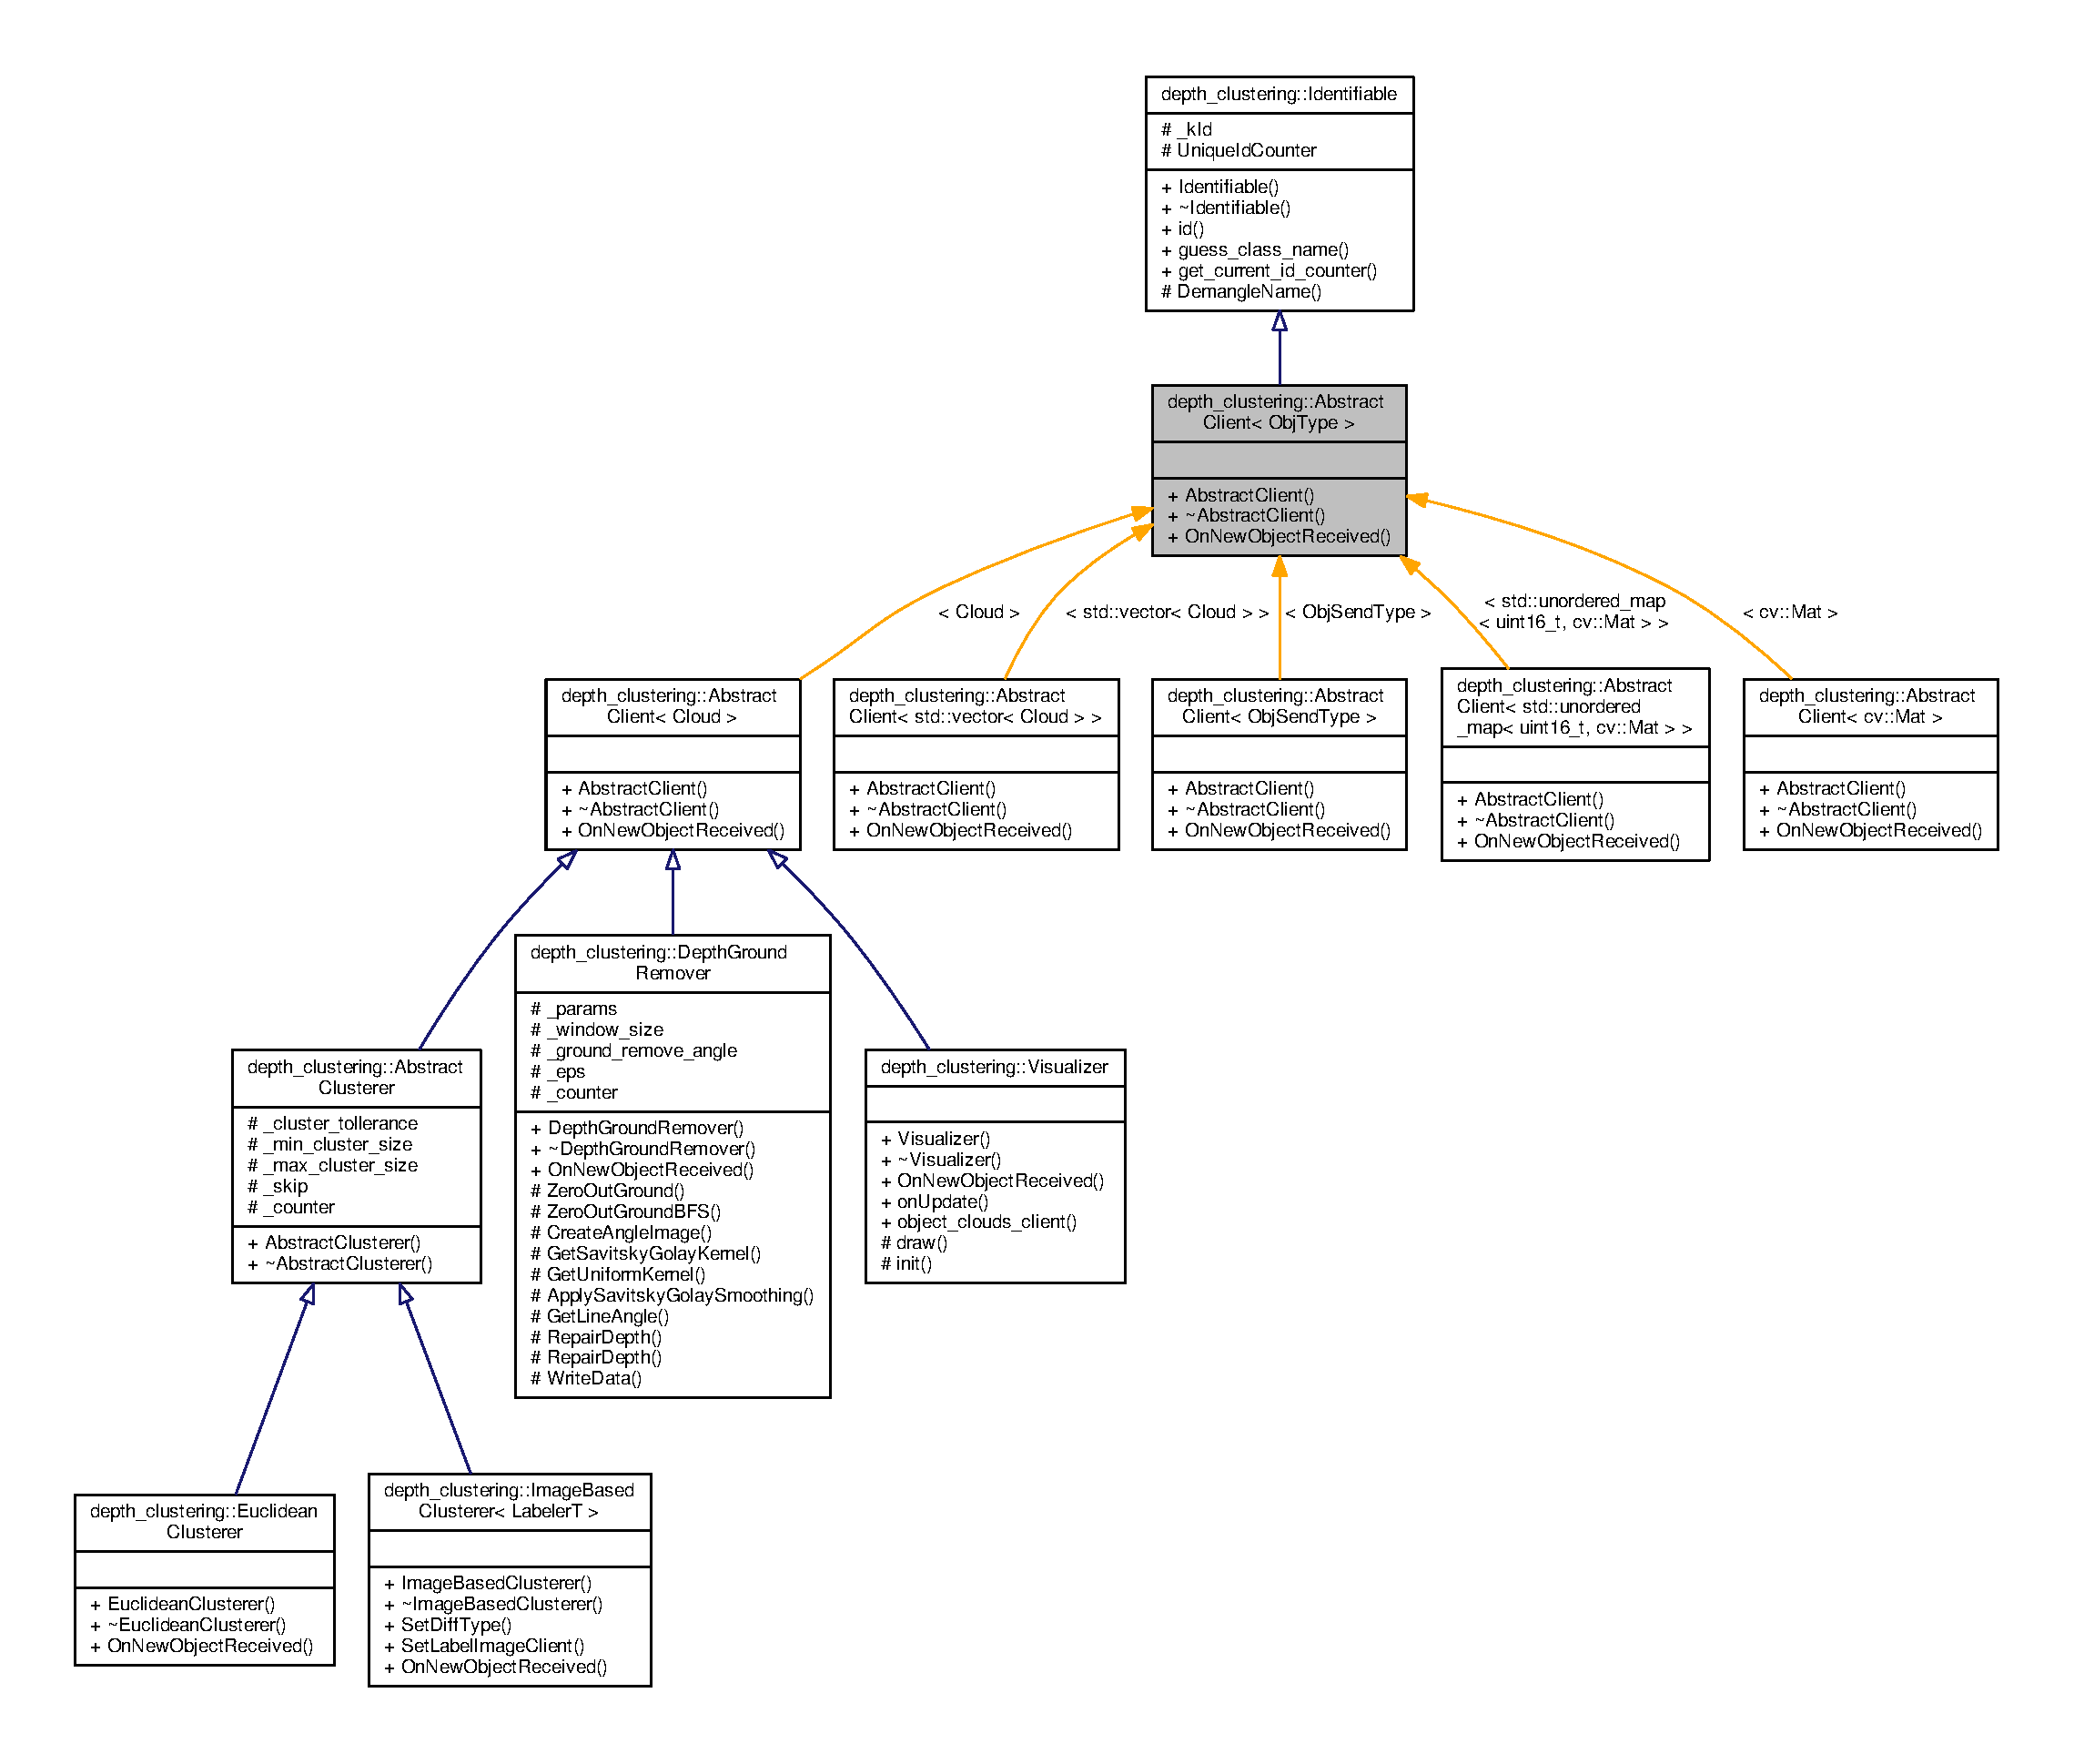
\includegraphics[width=350pt]{classdepth__clustering_1_1AbstractClient__inherit__graph}
\end{center}
\end{figure}


Collaboration diagram for depth\-\_\-clustering\-:\-:Abstract\-Client$<$ Obj\-Type $>$\-:
\nopagebreak
\begin{figure}[H]
\begin{center}
\leavevmode
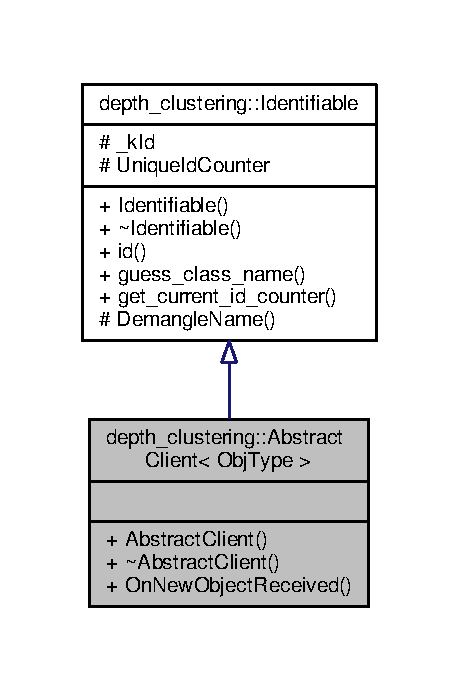
\includegraphics[width=220pt]{classdepth__clustering_1_1AbstractClient__coll__graph}
\end{center}
\end{figure}


The documentation for this class was generated from the following file\-:\begin{DoxyCompactItemize}
\item 
/home/hadoop/chy/depth\-\_\-clustering-\/master234/src/communication/abstract\-\_\-client.\-h\end{DoxyCompactItemize}

\hypertarget{classdepth__clustering_1_1AbstractClusterer}{\section{depth\-\_\-clustering\-:\-:Abstract\-Clusterer Class Reference}
\label{classdepth__clustering_1_1AbstractClusterer}\index{depth\-\_\-clustering\-::\-Abstract\-Clusterer@{depth\-\_\-clustering\-::\-Abstract\-Clusterer}}
}


Class for abstract clusterer.  




{\ttfamily \#include $<$abstract\-\_\-clusterer.\-h$>$}

\subsection*{Public Types}
\begin{DoxyCompactItemize}
\item 
\hypertarget{classdepth__clustering_1_1AbstractClusterer_a6417b572cb4d8e851fa5bb88eacfdeb4}{using {\bfseries Receiver} = \hyperlink{classdepth__clustering_1_1AbstractClient}{Abstract\-Client}$<$ \hyperlink{classdepth__clustering_1_1Cloud}{Cloud} $>$}\label{classdepth__clustering_1_1AbstractClusterer_a6417b572cb4d8e851fa5bb88eacfdeb4}

\item 
\hypertarget{classdepth__clustering_1_1AbstractClusterer_afbba93333487772e81cc718e183c1fe6}{using {\bfseries Sender} = \hyperlink{classdepth__clustering_1_1AbstractSender}{Abstract\-Sender}$<$ std\-::vector$<$ \hyperlink{classdepth__clustering_1_1Cloud}{Cloud} $>$$>$}\label{classdepth__clustering_1_1AbstractClusterer_afbba93333487772e81cc718e183c1fe6}

\end{DoxyCompactItemize}
\subsection*{Public Member Functions}
\begin{DoxyCompactItemize}
\item 
\hyperlink{classdepth__clustering_1_1AbstractClusterer_a6be8ef3c30066a96e1efa0f082634ed0}{Abstract\-Clusterer} (double cluster\-\_\-tollerance=0.\-2, uint16\-\_\-t min\-\_\-cluster\-\_\-size=100, uint16\-\_\-t max\-\_\-cluster\-\_\-size=25000, uint16\-\_\-t skip=10)
\begin{DoxyCompactList}\small\item\em Construct a clusterer. \end{DoxyCompactList}\end{DoxyCompactItemize}
\subsection*{Protected Attributes}
\begin{DoxyCompactItemize}
\item 
\hypertarget{classdepth__clustering_1_1AbstractClusterer_ae219f21aefc118debe4fc89dfb0af96a}{double {\bfseries \-\_\-cluster\-\_\-tollerance}}\label{classdepth__clustering_1_1AbstractClusterer_ae219f21aefc118debe4fc89dfb0af96a}

\item 
\hypertarget{classdepth__clustering_1_1AbstractClusterer_a7057f78c03aa9396850a61a92574f502}{uint16\-\_\-t {\bfseries \-\_\-min\-\_\-cluster\-\_\-size}}\label{classdepth__clustering_1_1AbstractClusterer_a7057f78c03aa9396850a61a92574f502}

\item 
\hypertarget{classdepth__clustering_1_1AbstractClusterer_ad11f0fd4ec9f7b83e9242d6fbbda0661}{uint16\-\_\-t {\bfseries \-\_\-max\-\_\-cluster\-\_\-size}}\label{classdepth__clustering_1_1AbstractClusterer_ad11f0fd4ec9f7b83e9242d6fbbda0661}

\item 
\hypertarget{classdepth__clustering_1_1AbstractClusterer_a4cc536460eb6ffb1d13cf2eba8039602}{uint16\-\_\-t {\bfseries \-\_\-skip}}\label{classdepth__clustering_1_1AbstractClusterer_a4cc536460eb6ffb1d13cf2eba8039602}

\item 
\hypertarget{classdepth__clustering_1_1AbstractClusterer_a951128009a13fde1a391289b359cdad2}{uint32\-\_\-t {\bfseries \-\_\-counter}}\label{classdepth__clustering_1_1AbstractClusterer_a951128009a13fde1a391289b359cdad2}

\end{DoxyCompactItemize}
\subsection*{Additional Inherited Members}


\subsection{Detailed Description}
Class for abstract clusterer. 

Inheritance diagram for depth\-\_\-clustering\-:\-:Abstract\-Clusterer\-:
\nopagebreak
\begin{figure}[H]
\begin{center}
\leavevmode
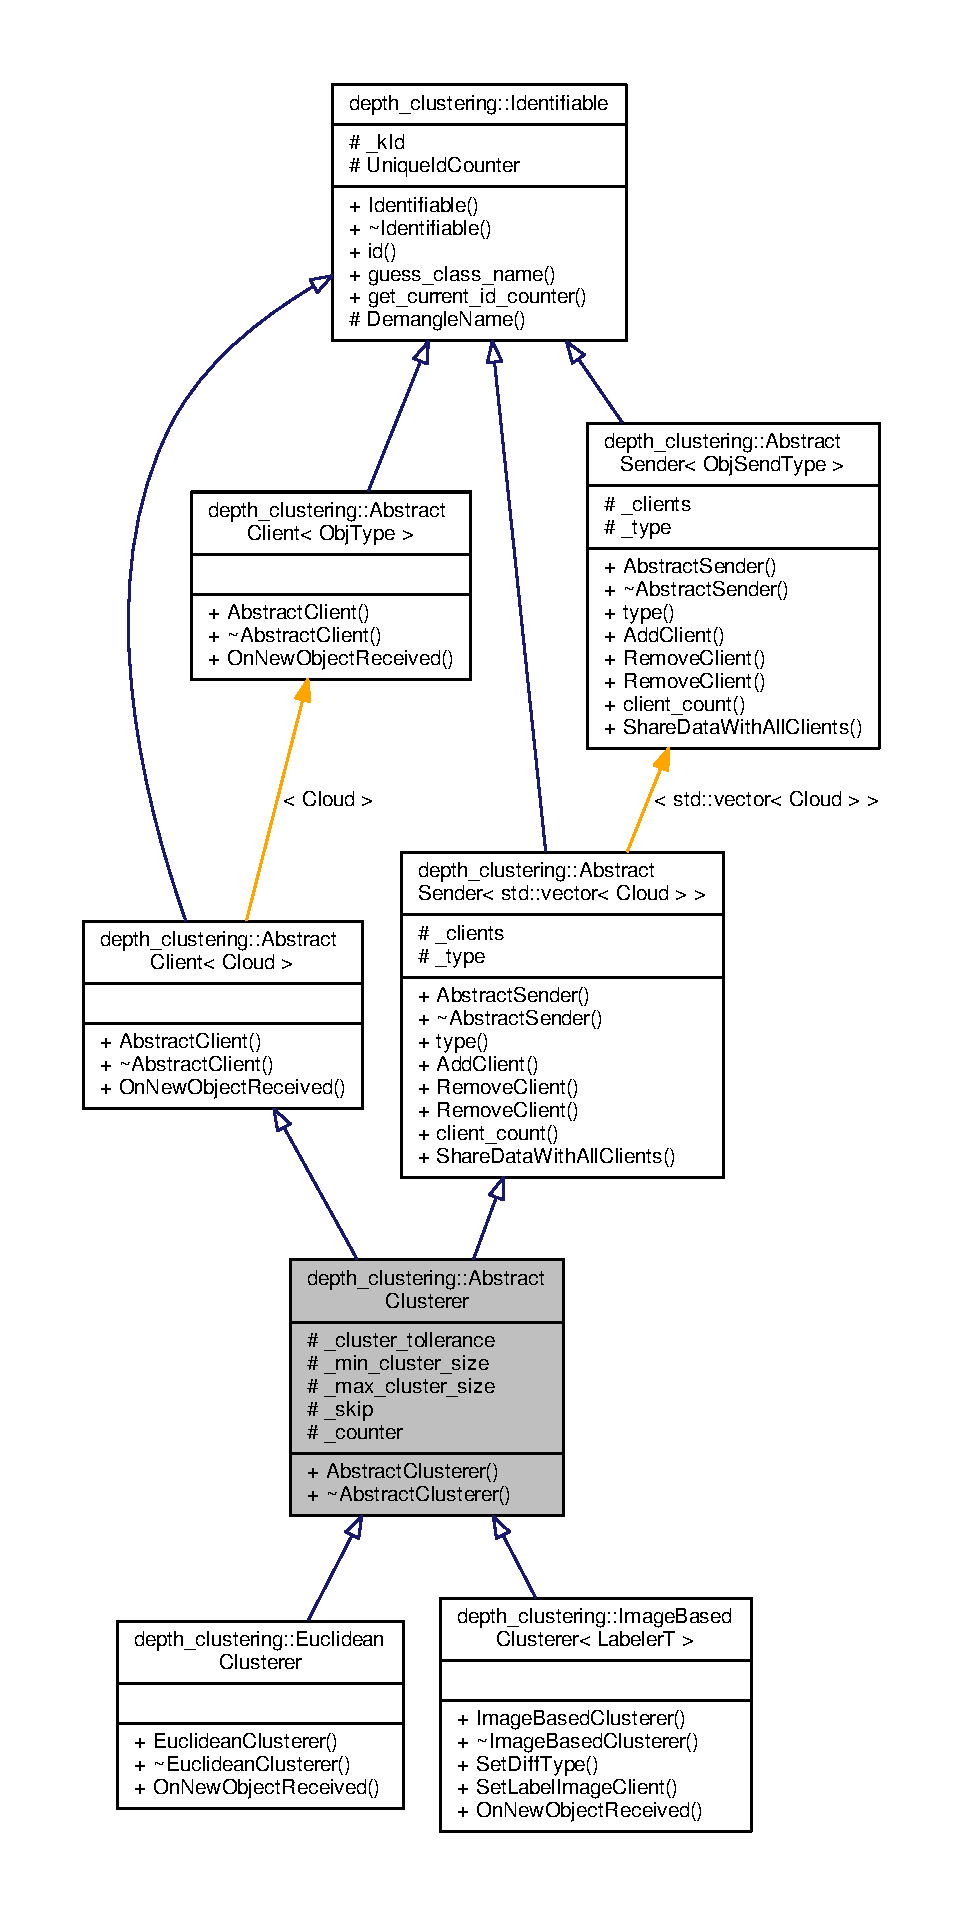
\includegraphics[height=550pt]{classdepth__clustering_1_1AbstractClusterer__inherit__graph}
\end{center}
\end{figure}


Collaboration diagram for depth\-\_\-clustering\-:\-:Abstract\-Clusterer\-:
\nopagebreak
\begin{figure}[H]
\begin{center}
\leavevmode
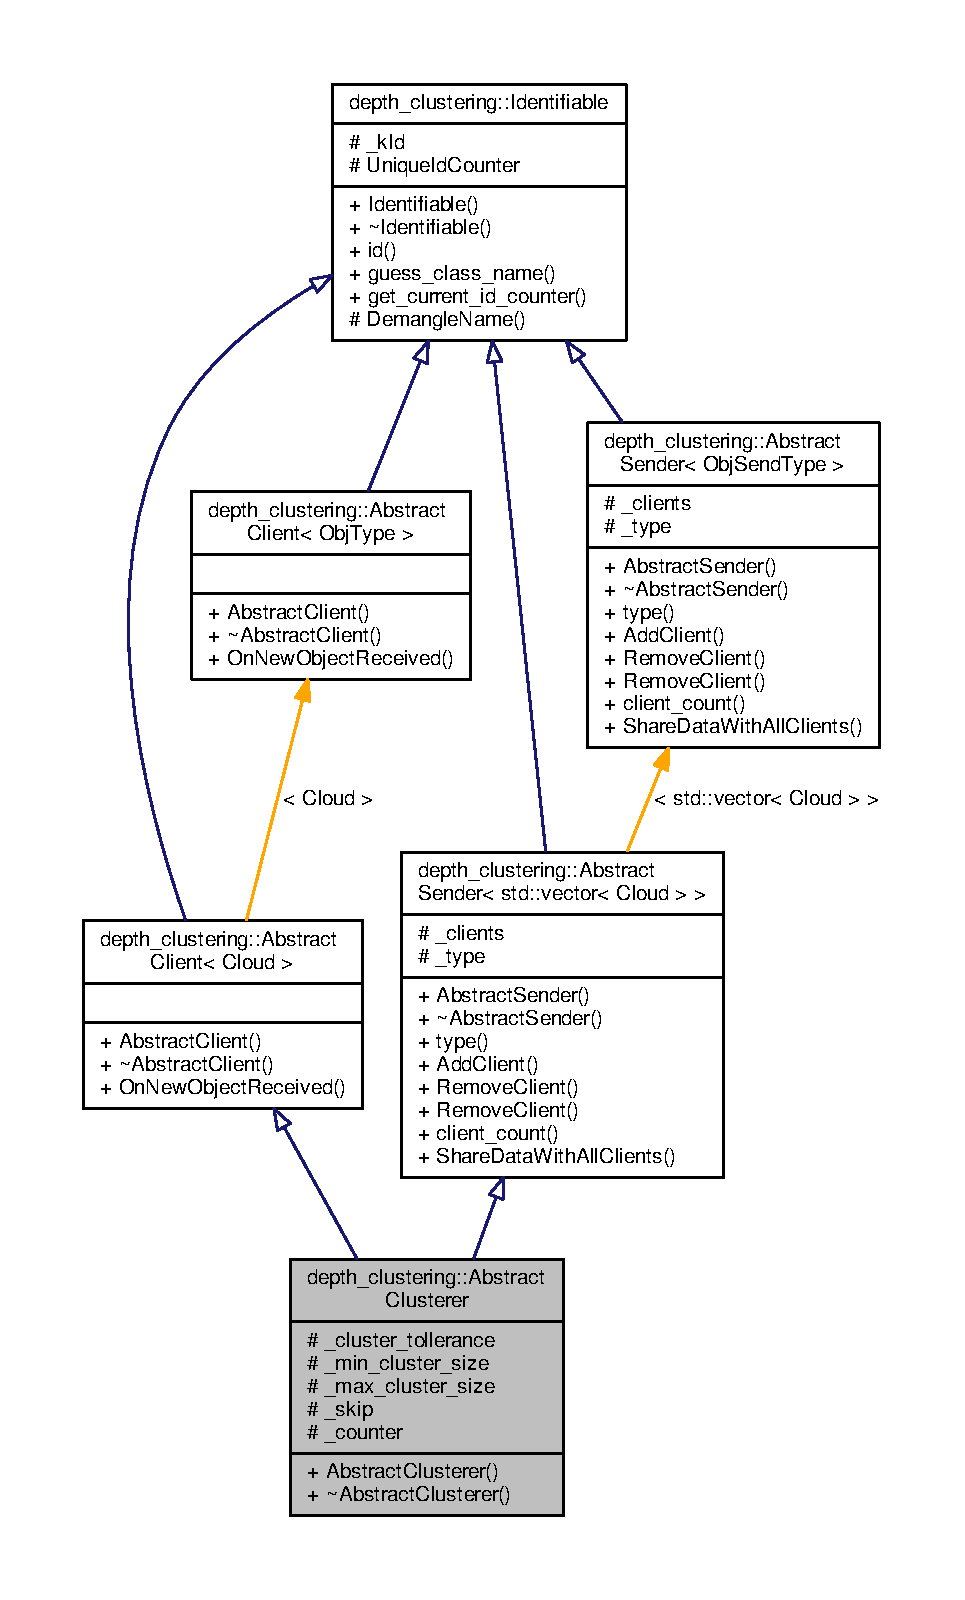
\includegraphics[height=550pt]{classdepth__clustering_1_1AbstractClusterer__coll__graph}
\end{center}
\end{figure}


\subsection{Constructor \& Destructor Documentation}
\hypertarget{classdepth__clustering_1_1AbstractClusterer_a6be8ef3c30066a96e1efa0f082634ed0}{\index{depth\-\_\-clustering\-::\-Abstract\-Clusterer@{depth\-\_\-clustering\-::\-Abstract\-Clusterer}!Abstract\-Clusterer@{Abstract\-Clusterer}}
\index{Abstract\-Clusterer@{Abstract\-Clusterer}!depth_clustering::AbstractClusterer@{depth\-\_\-clustering\-::\-Abstract\-Clusterer}}
\subsubsection[{Abstract\-Clusterer}]{\setlength{\rightskip}{0pt plus 5cm}depth\-\_\-clustering\-::\-Abstract\-Clusterer\-::\-Abstract\-Clusterer (
\begin{DoxyParamCaption}
\item[{double}]{cluster\-\_\-tollerance = {\ttfamily 0.2}, }
\item[{uint16\-\_\-t}]{min\-\_\-cluster\-\_\-size = {\ttfamily 100}, }
\item[{uint16\-\_\-t}]{max\-\_\-cluster\-\_\-size = {\ttfamily 25000}, }
\item[{uint16\-\_\-t}]{skip = {\ttfamily 10}}
\end{DoxyParamCaption}
)\hspace{0.3cm}{\ttfamily [inline]}, {\ttfamily [explicit]}}}\label{classdepth__clustering_1_1AbstractClusterer_a6be8ef3c30066a96e1efa0f082634ed0}


Construct a clusterer. 


\begin{DoxyParams}[1]{Parameters}
\mbox{\tt in}  & {\em cluster\-\_\-tollerance} & The cluster tollerance \\
\hline
\mbox{\tt in}  & {\em min\-\_\-cluster\-\_\-size} & The minimum cluster size \\
\hline
\mbox{\tt in}  & {\em max\-\_\-cluster\-\_\-size} & The maximum cluster size \\
\hline
\mbox{\tt in}  & {\em skip} & Only cluster every skip cloud \\
\hline
\end{DoxyParams}


The documentation for this class was generated from the following file\-:\begin{DoxyCompactItemize}
\item 
/home/hadoop/chy/depth\-\_\-clustering-\/master234/src/clusterers/abstract\-\_\-clusterer.\-h\end{DoxyCompactItemize}

\hypertarget{classdepth__clustering_1_1AbstractDiff}{\section{depth\-\_\-clustering\-:\-:Abstract\-Diff Class Reference}
\label{classdepth__clustering_1_1AbstractDiff}\index{depth\-\_\-clustering\-::\-Abstract\-Diff@{depth\-\_\-clustering\-::\-Abstract\-Diff}}
}


Class for abstract difference.  




{\ttfamily \#include $<$abstract\-\_\-diff.\-h$>$}

\subsection*{Public Member Functions}
\begin{DoxyCompactItemize}
\item 
\hyperlink{classdepth__clustering_1_1AbstractDiff_a14160500db5c2c1c1948a9e563318cc8}{Abstract\-Diff} (const cv\-::\-Mat $\ast$source\-\_\-image)
\begin{DoxyCompactList}\small\item\em construct a class with a source image pointer \end{DoxyCompactList}\item 
virtual float \hyperlink{classdepth__clustering_1_1AbstractDiff_a06ba188d8d83d0e4bad66c833656c26d}{Diff\-At} (const \hyperlink{structdepth__clustering_1_1PixelCoord}{Pixel\-Coord} \&from, const \hyperlink{structdepth__clustering_1_1PixelCoord}{Pixel\-Coord} \&to) const =0
\begin{DoxyCompactList}\small\item\em Gets diff between pixels from and to. \end{DoxyCompactList}\item 
virtual bool \hyperlink{classdepth__clustering_1_1AbstractDiff_a940280569ed86d8f7e95626b1a2312d7}{Satisfies\-Threshold} (float value, float threshold) const =0
\begin{DoxyCompactList}\small\item\em Does the difference satisfy a threshold? \end{DoxyCompactList}\item 
virtual cv\-::\-Mat \hyperlink{classdepth__clustering_1_1AbstractDiff_a5500c82f3e6800922ba6fc6c22c6d0bf}{Visualize} () const 
\begin{DoxyCompactList}\small\item\em Visualize the differences as a color image. \end{DoxyCompactList}\end{DoxyCompactItemize}
\subsection*{Protected Attributes}
\begin{DoxyCompactItemize}
\item 
\hypertarget{classdepth__clustering_1_1AbstractDiff_ac554e78b6f29341d1361a8ec6932698a}{const cv\-::\-Mat $\ast$ {\bfseries \-\_\-source\-\_\-image} = nullptr}\label{classdepth__clustering_1_1AbstractDiff_ac554e78b6f29341d1361a8ec6932698a}

\end{DoxyCompactItemize}


\subsection{Detailed Description}
Class for abstract difference. 

Inheritance diagram for depth\-\_\-clustering\-:\-:Abstract\-Diff\-:
\nopagebreak
\begin{figure}[H]
\begin{center}
\leavevmode
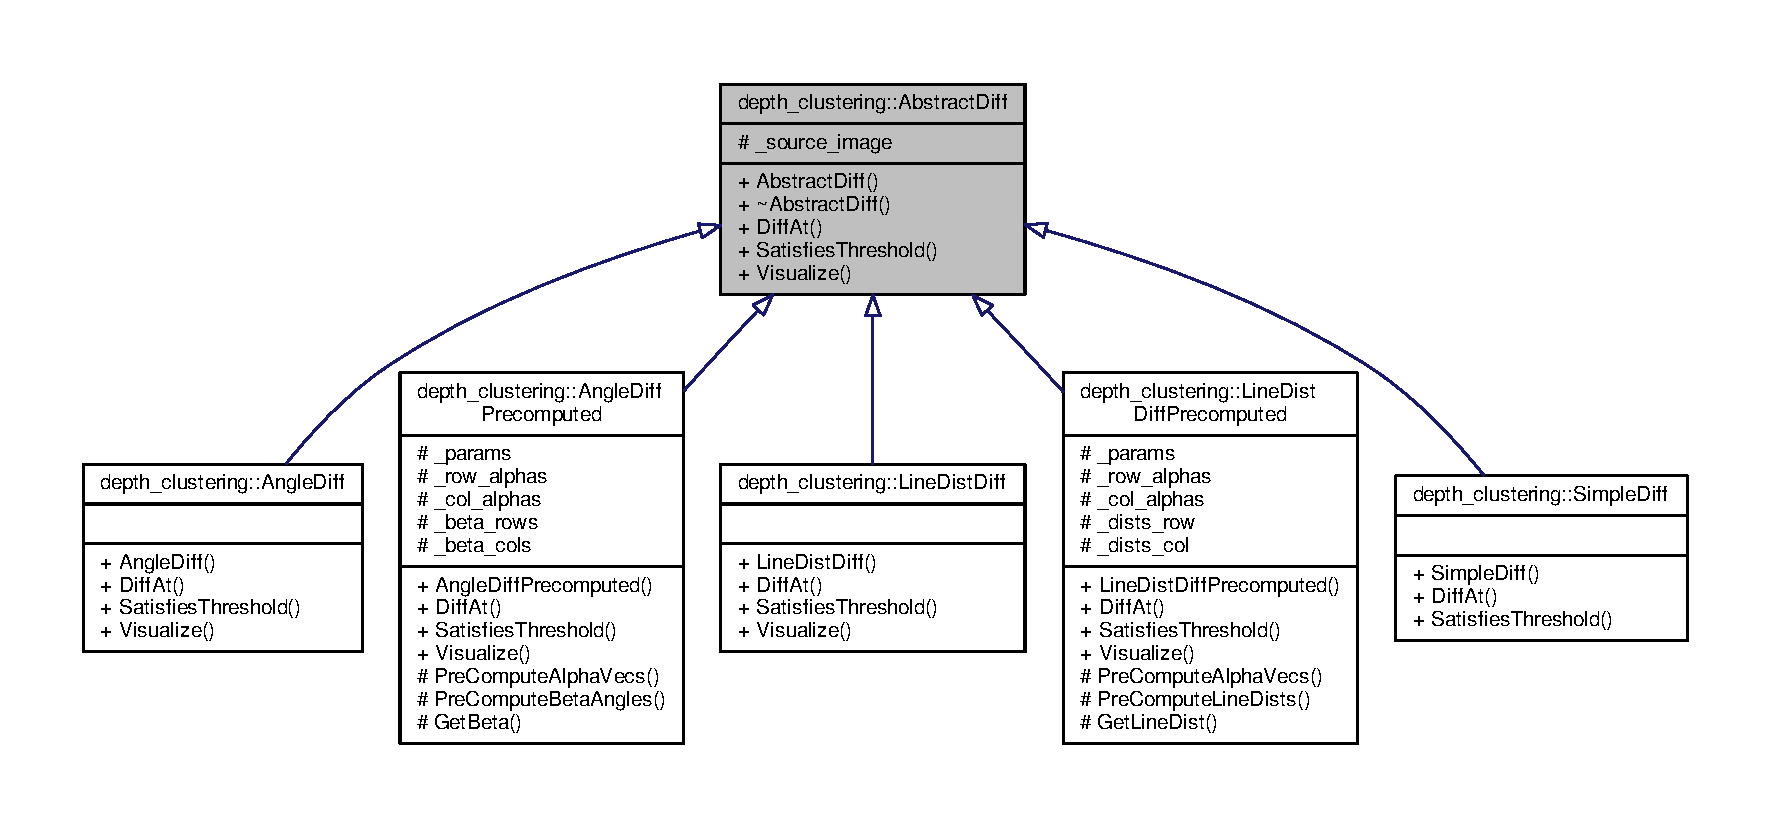
\includegraphics[width=350pt]{classdepth__clustering_1_1AbstractDiff__inherit__graph}
\end{center}
\end{figure}


Collaboration diagram for depth\-\_\-clustering\-:\-:Abstract\-Diff\-:
\nopagebreak
\begin{figure}[H]
\begin{center}
\leavevmode
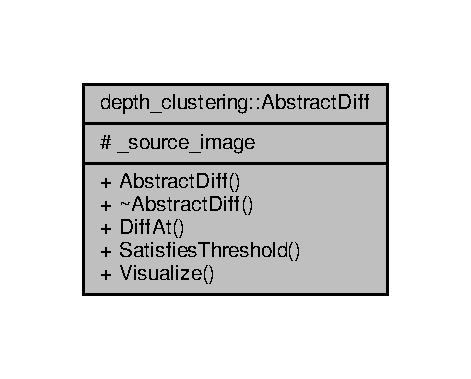
\includegraphics[width=226pt]{classdepth__clustering_1_1AbstractDiff__coll__graph}
\end{center}
\end{figure}


\subsection{Constructor \& Destructor Documentation}
\hypertarget{classdepth__clustering_1_1AbstractDiff_a14160500db5c2c1c1948a9e563318cc8}{\index{depth\-\_\-clustering\-::\-Abstract\-Diff@{depth\-\_\-clustering\-::\-Abstract\-Diff}!Abstract\-Diff@{Abstract\-Diff}}
\index{Abstract\-Diff@{Abstract\-Diff}!depth_clustering::AbstractDiff@{depth\-\_\-clustering\-::\-Abstract\-Diff}}
\subsubsection[{Abstract\-Diff}]{\setlength{\rightskip}{0pt plus 5cm}depth\-\_\-clustering\-::\-Abstract\-Diff\-::\-Abstract\-Diff (
\begin{DoxyParamCaption}
\item[{const cv\-::\-Mat $\ast$}]{source\-\_\-image}
\end{DoxyParamCaption}
)\hspace{0.3cm}{\ttfamily [inline]}, {\ttfamily [explicit]}}}\label{classdepth__clustering_1_1AbstractDiff_a14160500db5c2c1c1948a9e563318cc8}


construct a class with a source image pointer 


\begin{DoxyParams}[1]{Parameters}
\mbox{\tt in}  & {\em source\-\_\-image} & The source image pointer (C\-V\-\_\-32\-F type Mat) \\
\hline
\end{DoxyParams}


\subsection{Member Function Documentation}
\hypertarget{classdepth__clustering_1_1AbstractDiff_a06ba188d8d83d0e4bad66c833656c26d}{\index{depth\-\_\-clustering\-::\-Abstract\-Diff@{depth\-\_\-clustering\-::\-Abstract\-Diff}!Diff\-At@{Diff\-At}}
\index{Diff\-At@{Diff\-At}!depth_clustering::AbstractDiff@{depth\-\_\-clustering\-::\-Abstract\-Diff}}
\subsubsection[{Diff\-At}]{\setlength{\rightskip}{0pt plus 5cm}virtual float depth\-\_\-clustering\-::\-Abstract\-Diff\-::\-Diff\-At (
\begin{DoxyParamCaption}
\item[{const {\bf Pixel\-Coord} \&}]{from, }
\item[{const {\bf Pixel\-Coord} \&}]{to}
\end{DoxyParamCaption}
) const\hspace{0.3cm}{\ttfamily [pure virtual]}}}\label{classdepth__clustering_1_1AbstractDiff_a06ba188d8d83d0e4bad66c833656c26d}


Gets diff between pixels from and to. 


\begin{DoxyParams}[1]{Parameters}
\mbox{\tt in}  & {\em from} & pixel from which we want difference \\
\hline
\mbox{\tt in}  & {\em to} & pixel to which we want difference\\
\hline
\end{DoxyParams}
\begin{DoxyReturn}{Returns}
difference between the pixels 
\end{DoxyReturn}


Implemented in \hyperlink{classdepth__clustering_1_1LineDistDiffPrecomputed_ac505afaa537656af1bcc342ab1e910c4}{depth\-\_\-clustering\-::\-Line\-Dist\-Diff\-Precomputed}, \hyperlink{classdepth__clustering_1_1AngleDiffPrecomputed_ae15bb5fc9488ae2b26c77665931b8626}{depth\-\_\-clustering\-::\-Angle\-Diff\-Precomputed}, \hyperlink{classdepth__clustering_1_1LineDistDiff_a839eee44b14de26d85e6dbad5e37b356}{depth\-\_\-clustering\-::\-Line\-Dist\-Diff}, \hyperlink{classdepth__clustering_1_1AngleDiff_ac9bd0ec61ff0b213fd19235dc171c1c2}{depth\-\_\-clustering\-::\-Angle\-Diff}, and \hyperlink{classdepth__clustering_1_1SimpleDiff_a3afe28bd6a9cfbaff18e856a04d24824}{depth\-\_\-clustering\-::\-Simple\-Diff}.



Here is the caller graph for this function\-:
\nopagebreak
\begin{figure}[H]
\begin{center}
\leavevmode
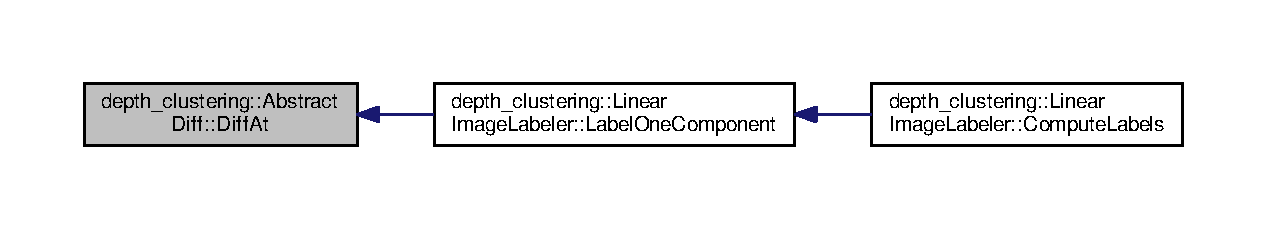
\includegraphics[width=350pt]{classdepth__clustering_1_1AbstractDiff_a06ba188d8d83d0e4bad66c833656c26d_icgraph}
\end{center}
\end{figure}


\hypertarget{classdepth__clustering_1_1AbstractDiff_a940280569ed86d8f7e95626b1a2312d7}{\index{depth\-\_\-clustering\-::\-Abstract\-Diff@{depth\-\_\-clustering\-::\-Abstract\-Diff}!Satisfies\-Threshold@{Satisfies\-Threshold}}
\index{Satisfies\-Threshold@{Satisfies\-Threshold}!depth_clustering::AbstractDiff@{depth\-\_\-clustering\-::\-Abstract\-Diff}}
\subsubsection[{Satisfies\-Threshold}]{\setlength{\rightskip}{0pt plus 5cm}virtual bool depth\-\_\-clustering\-::\-Abstract\-Diff\-::\-Satisfies\-Threshold (
\begin{DoxyParamCaption}
\item[{float}]{value, }
\item[{float}]{threshold}
\end{DoxyParamCaption}
) const\hspace{0.3cm}{\ttfamily [pure virtual]}}}\label{classdepth__clustering_1_1AbstractDiff_a940280569ed86d8f7e95626b1a2312d7}


Does the difference satisfy a threshold? 


\begin{DoxyParams}[1]{Parameters}
\mbox{\tt in}  & {\em value} & Query value \\
\hline
\mbox{\tt in}  & {\em threshold} & The threshold\\
\hline
\end{DoxyParams}
\begin{DoxyReturn}{Returns}
true if satisfies, false, otherwise 
\end{DoxyReturn}


Implemented in \hyperlink{classdepth__clustering_1_1LineDistDiffPrecomputed_ac3ce8196d5e6f49f3e3bdc3e3b32b033}{depth\-\_\-clustering\-::\-Line\-Dist\-Diff\-Precomputed}, \hyperlink{classdepth__clustering_1_1AngleDiffPrecomputed_a28a32c0cb0405163fe237909fe5f6c0c}{depth\-\_\-clustering\-::\-Angle\-Diff\-Precomputed}, \hyperlink{classdepth__clustering_1_1LineDistDiff_ae9debede2cffd6bb40ca4c4a82c52f61}{depth\-\_\-clustering\-::\-Line\-Dist\-Diff}, \hyperlink{classdepth__clustering_1_1AngleDiff_ac65e8f42b1f2ac82db14ebe188c004a2}{depth\-\_\-clustering\-::\-Angle\-Diff}, and \hyperlink{classdepth__clustering_1_1SimpleDiff_a277c862d4ffdf1bfc24bd1bd70cb98a7}{depth\-\_\-clustering\-::\-Simple\-Diff}.



Here is the caller graph for this function\-:
\nopagebreak
\begin{figure}[H]
\begin{center}
\leavevmode
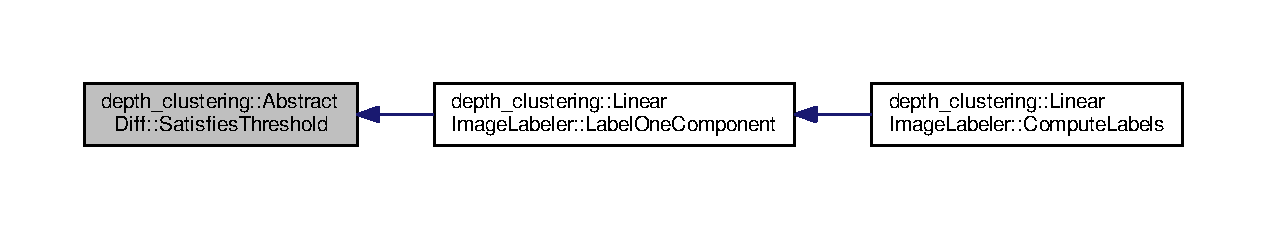
\includegraphics[width=350pt]{classdepth__clustering_1_1AbstractDiff_a940280569ed86d8f7e95626b1a2312d7_icgraph}
\end{center}
\end{figure}


\hypertarget{classdepth__clustering_1_1AbstractDiff_a5500c82f3e6800922ba6fc6c22c6d0bf}{\index{depth\-\_\-clustering\-::\-Abstract\-Diff@{depth\-\_\-clustering\-::\-Abstract\-Diff}!Visualize@{Visualize}}
\index{Visualize@{Visualize}!depth_clustering::AbstractDiff@{depth\-\_\-clustering\-::\-Abstract\-Diff}}
\subsubsection[{Visualize}]{\setlength{\rightskip}{0pt plus 5cm}virtual cv\-::\-Mat depth\-\_\-clustering\-::\-Abstract\-Diff\-::\-Visualize (
\begin{DoxyParamCaption}
{}
\end{DoxyParamCaption}
) const\hspace{0.3cm}{\ttfamily [inline]}, {\ttfamily [virtual]}}}\label{classdepth__clustering_1_1AbstractDiff_a5500c82f3e6800922ba6fc6c22c6d0bf}


Visualize the differences as a color image. 

\begin{DoxyReturn}{Returns}
Open\-C\-V Mat of type C\-V\-\_\-8\-U\-C3 to visualize differences in color. 
\end{DoxyReturn}


Reimplemented in \hyperlink{classdepth__clustering_1_1LineDistDiffPrecomputed_ae06f8b4dd6330730849725c1b1f20b43}{depth\-\_\-clustering\-::\-Line\-Dist\-Diff\-Precomputed}, \hyperlink{classdepth__clustering_1_1AngleDiffPrecomputed_a35da8cd9455b3485acfd5da203ecaafb}{depth\-\_\-clustering\-::\-Angle\-Diff\-Precomputed}, \hyperlink{classdepth__clustering_1_1LineDistDiff_a7feaf820589ccfb47786d5124a74d725}{depth\-\_\-clustering\-::\-Line\-Dist\-Diff}, and \hyperlink{classdepth__clustering_1_1AngleDiff_a462e4aadd35ca06e9b061d08c9787074}{depth\-\_\-clustering\-::\-Angle\-Diff}.



The documentation for this class was generated from the following file\-:\begin{DoxyCompactItemize}
\item 
/home/hadoop/chy/depth\-\_\-clustering-\/master234/src/image\-\_\-labelers/diff\-\_\-helpers/abstract\-\_\-diff.\-h\end{DoxyCompactItemize}

\hypertarget{classdepth__clustering_1_1AbstractImageLabeler}{\section{depth\-\_\-clustering\-:\-:Abstract\-Image\-Labeler Class Reference}
\label{classdepth__clustering_1_1AbstractImageLabeler}\index{depth\-\_\-clustering\-::\-Abstract\-Image\-Labeler@{depth\-\_\-clustering\-::\-Abstract\-Image\-Labeler}}
}


Class for abstract image labeler.  




{\ttfamily \#include $<$abstract\-\_\-image\-\_\-labeler.\-h$>$}

\subsection*{Public Member Functions}
\begin{DoxyCompactItemize}
\item 
\hypertarget{classdepth__clustering_1_1AbstractImageLabeler_ac01889e0a3d088cf7627809f4d8aab19}{{\bfseries Abstract\-Image\-Labeler} (const cv\-::\-Mat \&depth\-\_\-image, const \hyperlink{classdepth__clustering_1_1ProjectionParams}{Projection\-Params} \&params, const Radians \&angle\-\_\-threshold)}\label{classdepth__clustering_1_1AbstractImageLabeler_ac01889e0a3d088cf7627809f4d8aab19}

\item 
\hypertarget{classdepth__clustering_1_1AbstractImageLabeler_a28e8e094c9a47a02a2ce9eabef9526e6}{void {\bfseries Set\-Depth\-Image} (const cv\-::\-Mat \&depth\-\_\-image)}\label{classdepth__clustering_1_1AbstractImageLabeler_a28e8e094c9a47a02a2ce9eabef9526e6}

\item 
\hypertarget{classdepth__clustering_1_1AbstractImageLabeler_ac66f0554e1c988ab0bf413a2f17d3905}{virtual void \hyperlink{classdepth__clustering_1_1AbstractImageLabeler_ac66f0554e1c988ab0bf413a2f17d3905}{Compute\-Labels} (Diff\-Factory\-::\-Diff\-Type diff\-\_\-type)=0}\label{classdepth__clustering_1_1AbstractImageLabeler_ac66f0554e1c988ab0bf413a2f17d3905}

\begin{DoxyCompactList}\small\item\em An interface for children to compute labels //为了给他的继承的值来进行加入标签 \end{DoxyCompactList}\item 
const cv\-::\-Mat $\ast$ \hyperlink{classdepth__clustering_1_1AbstractImageLabeler_abc25b75282cce43684e2a469e647d83b}{Get\-Label\-Image} () const 
\begin{DoxyCompactList}\small\item\em Gets the label image. \end{DoxyCompactList}\end{DoxyCompactItemize}
\subsection*{Static Public Member Functions}
\begin{DoxyCompactItemize}
\item 
static cv\-::\-Mat \hyperlink{classdepth__clustering_1_1AbstractImageLabeler_abab18e0c1ca40b54922a2f21948b996b}{Labels\-To\-Color} (const cv\-::\-Mat \&label\-\_\-image)
\begin{DoxyCompactList}\small\item\em Generates random-\/colored image from image of labels. \end{DoxyCompactList}\end{DoxyCompactItemize}
\subsection*{Protected Attributes}
\begin{DoxyCompactItemize}
\item 
\hypertarget{classdepth__clustering_1_1AbstractImageLabeler_adb50d2beeba4e4eac26b5ace9304728b}{const cv\-::\-Mat $\ast$ {\bfseries \-\_\-depth\-\_\-image\-\_\-ptr}}\label{classdepth__clustering_1_1AbstractImageLabeler_adb50d2beeba4e4eac26b5ace9304728b}

\item 
\hypertarget{classdepth__clustering_1_1AbstractImageLabeler_a25fcaead9f8806fa75ad44c669e2a518}{\hyperlink{classdepth__clustering_1_1ProjectionParams}{Projection\-Params} {\bfseries \-\_\-params}}\label{classdepth__clustering_1_1AbstractImageLabeler_a25fcaead9f8806fa75ad44c669e2a518}

\item 
\hypertarget{classdepth__clustering_1_1AbstractImageLabeler_aeabb8ac8238c684066f8c0edcca9b807}{cv\-::\-Mat {\bfseries \-\_\-label\-\_\-image}}\label{classdepth__clustering_1_1AbstractImageLabeler_aeabb8ac8238c684066f8c0edcca9b807}

\item 
\hypertarget{classdepth__clustering_1_1AbstractImageLabeler_a1a338d254a41ba94bd4122aa006fbe57}{float {\bfseries \-\_\-radians\-\_\-threshold}}\label{classdepth__clustering_1_1AbstractImageLabeler_a1a338d254a41ba94bd4122aa006fbe57}

\end{DoxyCompactItemize}
\subsection*{Static Protected Attributes}
\begin{DoxyCompactItemize}
\item 
\hypertarget{classdepth__clustering_1_1AbstractImageLabeler_a24ea9d1c40b872189a9e93f369ae34b2}{static constexpr std\-::array\\*
$<$ std\-::array$<$ int, 3 $>$, 200 $>$ {\bfseries R\-A\-N\-D\-O\-M\-\_\-\-C\-O\-L\-O\-R\-S}}\label{classdepth__clustering_1_1AbstractImageLabeler_a24ea9d1c40b872189a9e93f369ae34b2}

\end{DoxyCompactItemize}


\subsection{Detailed Description}
Class for abstract image labeler. 

This class is responsible for labeling an given depth image based on the provided angle\-\_\-threshold.//在给定的角度阈值中来对深度图像进行加入标签 

Inheritance diagram for depth\-\_\-clustering\-:\-:Abstract\-Image\-Labeler\-:
\nopagebreak
\begin{figure}[H]
\begin{center}
\leavevmode
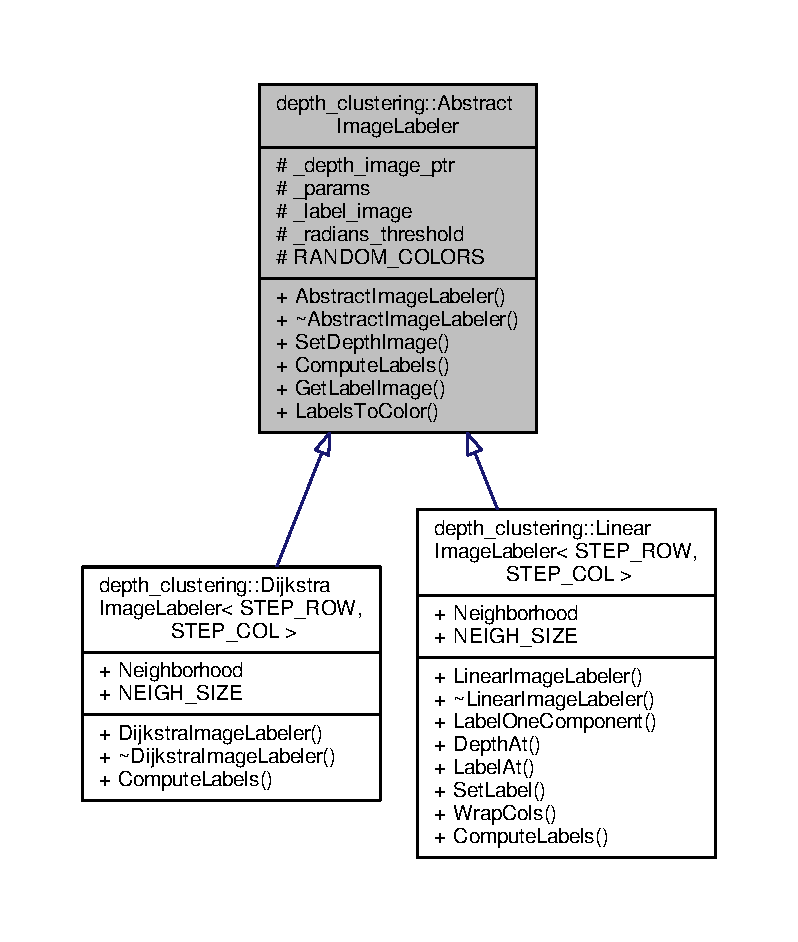
\includegraphics[width=350pt]{classdepth__clustering_1_1AbstractImageLabeler__inherit__graph}
\end{center}
\end{figure}


Collaboration diagram for depth\-\_\-clustering\-:\-:Abstract\-Image\-Labeler\-:
\nopagebreak
\begin{figure}[H]
\begin{center}
\leavevmode
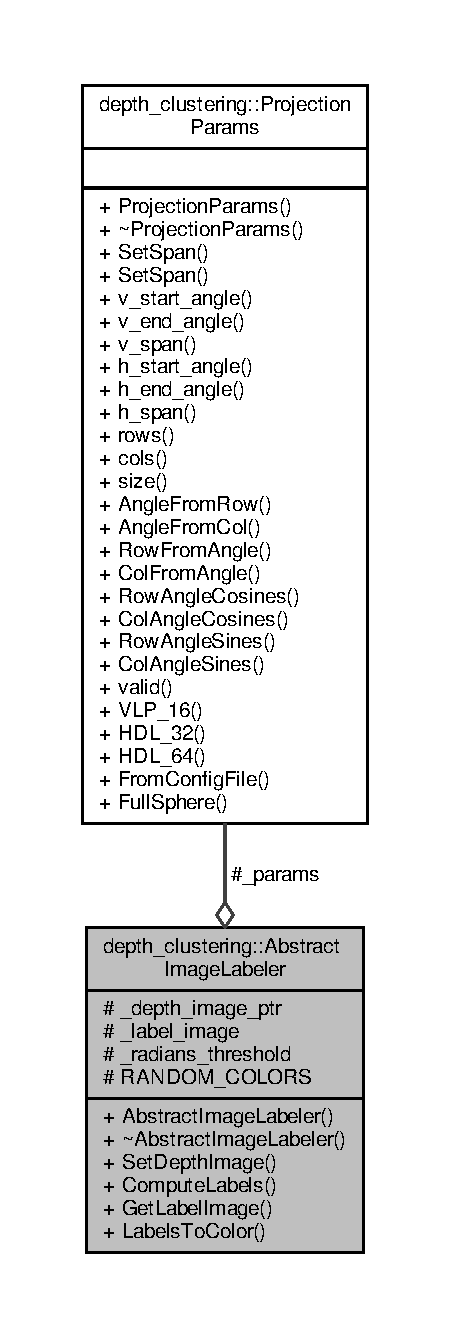
\includegraphics[height=550pt]{classdepth__clustering_1_1AbstractImageLabeler__coll__graph}
\end{center}
\end{figure}


\subsection{Member Function Documentation}
\hypertarget{classdepth__clustering_1_1AbstractImageLabeler_abc25b75282cce43684e2a469e647d83b}{\index{depth\-\_\-clustering\-::\-Abstract\-Image\-Labeler@{depth\-\_\-clustering\-::\-Abstract\-Image\-Labeler}!Get\-Label\-Image@{Get\-Label\-Image}}
\index{Get\-Label\-Image@{Get\-Label\-Image}!depth_clustering::AbstractImageLabeler@{depth\-\_\-clustering\-::\-Abstract\-Image\-Labeler}}
\subsubsection[{Get\-Label\-Image}]{\setlength{\rightskip}{0pt plus 5cm}const cv\-::\-Mat$\ast$ depth\-\_\-clustering\-::\-Abstract\-Image\-Labeler\-::\-Get\-Label\-Image (
\begin{DoxyParamCaption}
{}
\end{DoxyParamCaption}
) const\hspace{0.3cm}{\ttfamily [inline]}}}\label{classdepth__clustering_1_1AbstractImageLabeler_abc25b75282cce43684e2a469e647d83b}


Gets the label image. 

\begin{DoxyReturn}{Returns}
The label image. 
\end{DoxyReturn}
\hypertarget{classdepth__clustering_1_1AbstractImageLabeler_abab18e0c1ca40b54922a2f21948b996b}{\index{depth\-\_\-clustering\-::\-Abstract\-Image\-Labeler@{depth\-\_\-clustering\-::\-Abstract\-Image\-Labeler}!Labels\-To\-Color@{Labels\-To\-Color}}
\index{Labels\-To\-Color@{Labels\-To\-Color}!depth_clustering::AbstractImageLabeler@{depth\-\_\-clustering\-::\-Abstract\-Image\-Labeler}}
\subsubsection[{Labels\-To\-Color}]{\setlength{\rightskip}{0pt plus 5cm}Mat depth\-\_\-clustering\-::\-Abstract\-Image\-Labeler\-::\-Labels\-To\-Color (
\begin{DoxyParamCaption}
\item[{const cv\-::\-Mat \&}]{label\-\_\-image}
\end{DoxyParamCaption}
)\hspace{0.3cm}{\ttfamily [static]}}}\label{classdepth__clustering_1_1AbstractImageLabeler_abab18e0c1ca40b54922a2f21948b996b}


Generates random-\/colored image from image of labels. 


\begin{DoxyParams}[1]{Parameters}
\mbox{\tt in}  & {\em label\-\_\-image} & The label image\\
\hline
\end{DoxyParams}
\begin{DoxyReturn}{Returns}
Random-\/colored image from label image 
\end{DoxyReturn}


Here is the caller graph for this function\-:
\nopagebreak
\begin{figure}[H]
\begin{center}
\leavevmode
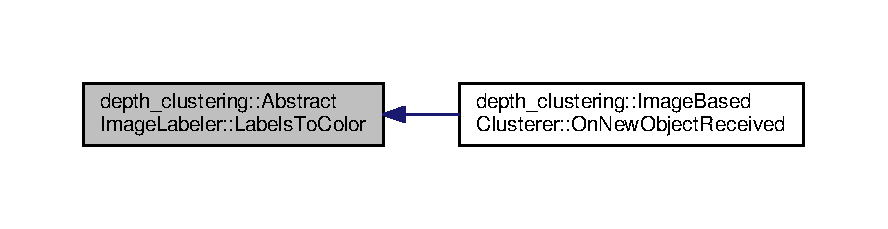
\includegraphics[width=350pt]{classdepth__clustering_1_1AbstractImageLabeler_abab18e0c1ca40b54922a2f21948b996b_icgraph}
\end{center}
\end{figure}




The documentation for this class was generated from the following files\-:\begin{DoxyCompactItemize}
\item 
/home/hadoop/chy/depth\-\_\-clustering-\/master234/src/image\-\_\-labelers/abstract\-\_\-image\-\_\-labeler.\-h\item 
/home/hadoop/chy/depth\-\_\-clustering-\/master234/src/image\-\_\-labelers/abstract\-\_\-image\-\_\-labeler.\-cpp\end{DoxyCompactItemize}

\hypertarget{classdepth__clustering_1_1AbstractSender}{\section{depth\-\_\-clustering\-:\-:Abstract\-Sender$<$ Obj\-Send\-Type $>$ Class Template Reference}
\label{classdepth__clustering_1_1AbstractSender}\index{depth\-\_\-clustering\-::\-Abstract\-Sender$<$ Obj\-Send\-Type $>$@{depth\-\_\-clustering\-::\-Abstract\-Sender$<$ Obj\-Send\-Type $>$}}
}


Class for abstract sender.  




{\ttfamily \#include $<$abstract\-\_\-sender.\-h$>$}

\subsection*{Public Member Functions}
\begin{DoxyCompactItemize}
\item 
\hypertarget{classdepth__clustering_1_1AbstractSender_ab04a328c2cc29a97bc3bba2b696c8786}{{\bfseries Abstract\-Sender} (Sender\-Type \hyperlink{classdepth__clustering_1_1AbstractSender_ad9da304185f766eb4b0035d6610caa49}{type}=Sender\-Type\-::\-U\-N\-D\-E\-F\-I\-N\-E\-D)}\label{classdepth__clustering_1_1AbstractSender_ab04a328c2cc29a97bc3bba2b696c8786}

\item 
const char $\ast$ \hyperlink{classdepth__clustering_1_1AbstractSender_ad9da304185f766eb4b0035d6610caa49}{type} () const 
\begin{DoxyCompactList}\small\item\em Gets type of sender as string. \end{DoxyCompactList}\item 
void \hyperlink{classdepth__clustering_1_1AbstractSender_aca33c29cca1916fb0a3edd9024a49b51}{Add\-Client} (\hyperlink{classdepth__clustering_1_1AbstractClient}{Abstract\-Client}$<$ Obj\-Send\-Type $>$ $\ast$client)
\begin{DoxyCompactList}\small\item\em Adds a client. \end{DoxyCompactList}\item 
void \hyperlink{classdepth__clustering_1_1AbstractSender_a0c33c98abe8fa71a86f02af95b1c71c1}{Remove\-Client} (int \hyperlink{classdepth__clustering_1_1Identifiable_a020b49a5102a2ef0eec7b9e74add7669}{id})
\begin{DoxyCompactList}\small\item\em Removes a client. \end{DoxyCompactList}\item 
\hypertarget{classdepth__clustering_1_1AbstractSender_ab331127e3e36b15413e1eecf55b5b284}{void {\bfseries Remove\-Client} (\hyperlink{classdepth__clustering_1_1AbstractClient}{Abstract\-Client}$<$ Obj\-Send\-Type $>$ $\ast$client)}\label{classdepth__clustering_1_1AbstractSender_ab331127e3e36b15413e1eecf55b5b284}

\item 
size\-\_\-t \hyperlink{classdepth__clustering_1_1AbstractSender_a957331eb41f11208bbe6174895c11bf2}{client\-\_\-count} ()
\begin{DoxyCompactList}\small\item\em Get number of clients currently subscribed. \end{DoxyCompactList}\item 
void \hyperlink{classdepth__clustering_1_1AbstractSender_a147752e5ab7ca15da9c8d8e60575390b}{Share\-Data\-With\-All\-Clients} (const Obj\-Send\-Type \&obj, int \hyperlink{classdepth__clustering_1_1Identifiable_a020b49a5102a2ef0eec7b9e74add7669}{id}=-\/1)
\begin{DoxyCompactList}\small\item\em Shares data with everyone who listens to it. \end{DoxyCompactList}\end{DoxyCompactItemize}
\subsection*{Protected Types}
\begin{DoxyCompactItemize}
\item 
\hypertarget{classdepth__clustering_1_1AbstractSender_adc736ec9622d4baf520c8379a23e65ab}{using {\bfseries Id\-Client\-Mapping} = std\-::map$<$ int, \hyperlink{classdepth__clustering_1_1AbstractClient}{Abstract\-Client}$<$ Obj\-Send\-Type $>$ $\ast$ $>$}\label{classdepth__clustering_1_1AbstractSender_adc736ec9622d4baf520c8379a23e65ab}

\end{DoxyCompactItemize}
\subsection*{Protected Attributes}
\begin{DoxyCompactItemize}
\item 
\hypertarget{classdepth__clustering_1_1AbstractSender_a5ef5e33f2a4a2821b2eb4285fe85f80e}{Id\-Client\-Mapping {\bfseries \-\_\-clients}}\label{classdepth__clustering_1_1AbstractSender_a5ef5e33f2a4a2821b2eb4285fe85f80e}

\item 
\hypertarget{classdepth__clustering_1_1AbstractSender_a9c837623381f9ec0e26130457286af1a}{Sender\-Type {\bfseries \-\_\-type}}\label{classdepth__clustering_1_1AbstractSender_a9c837623381f9ec0e26130457286af1a}

\end{DoxyCompactItemize}
\subsection*{Additional Inherited Members}


\subsection{Detailed Description}
\subsubsection*{template$<$class Obj\-Send\-Type$>$class depth\-\_\-clustering\-::\-Abstract\-Sender$<$ Obj\-Send\-Type $>$}

Class for abstract sender. 


\begin{DoxyTemplParams}{Template Parameters}
{\em Obj\-Send\-Type} & Type of the object to be sent. \\
\hline
\end{DoxyTemplParams}


Inheritance diagram for depth\-\_\-clustering\-:\-:Abstract\-Sender$<$ Obj\-Send\-Type $>$\-:
\nopagebreak
\begin{figure}[H]
\begin{center}
\leavevmode
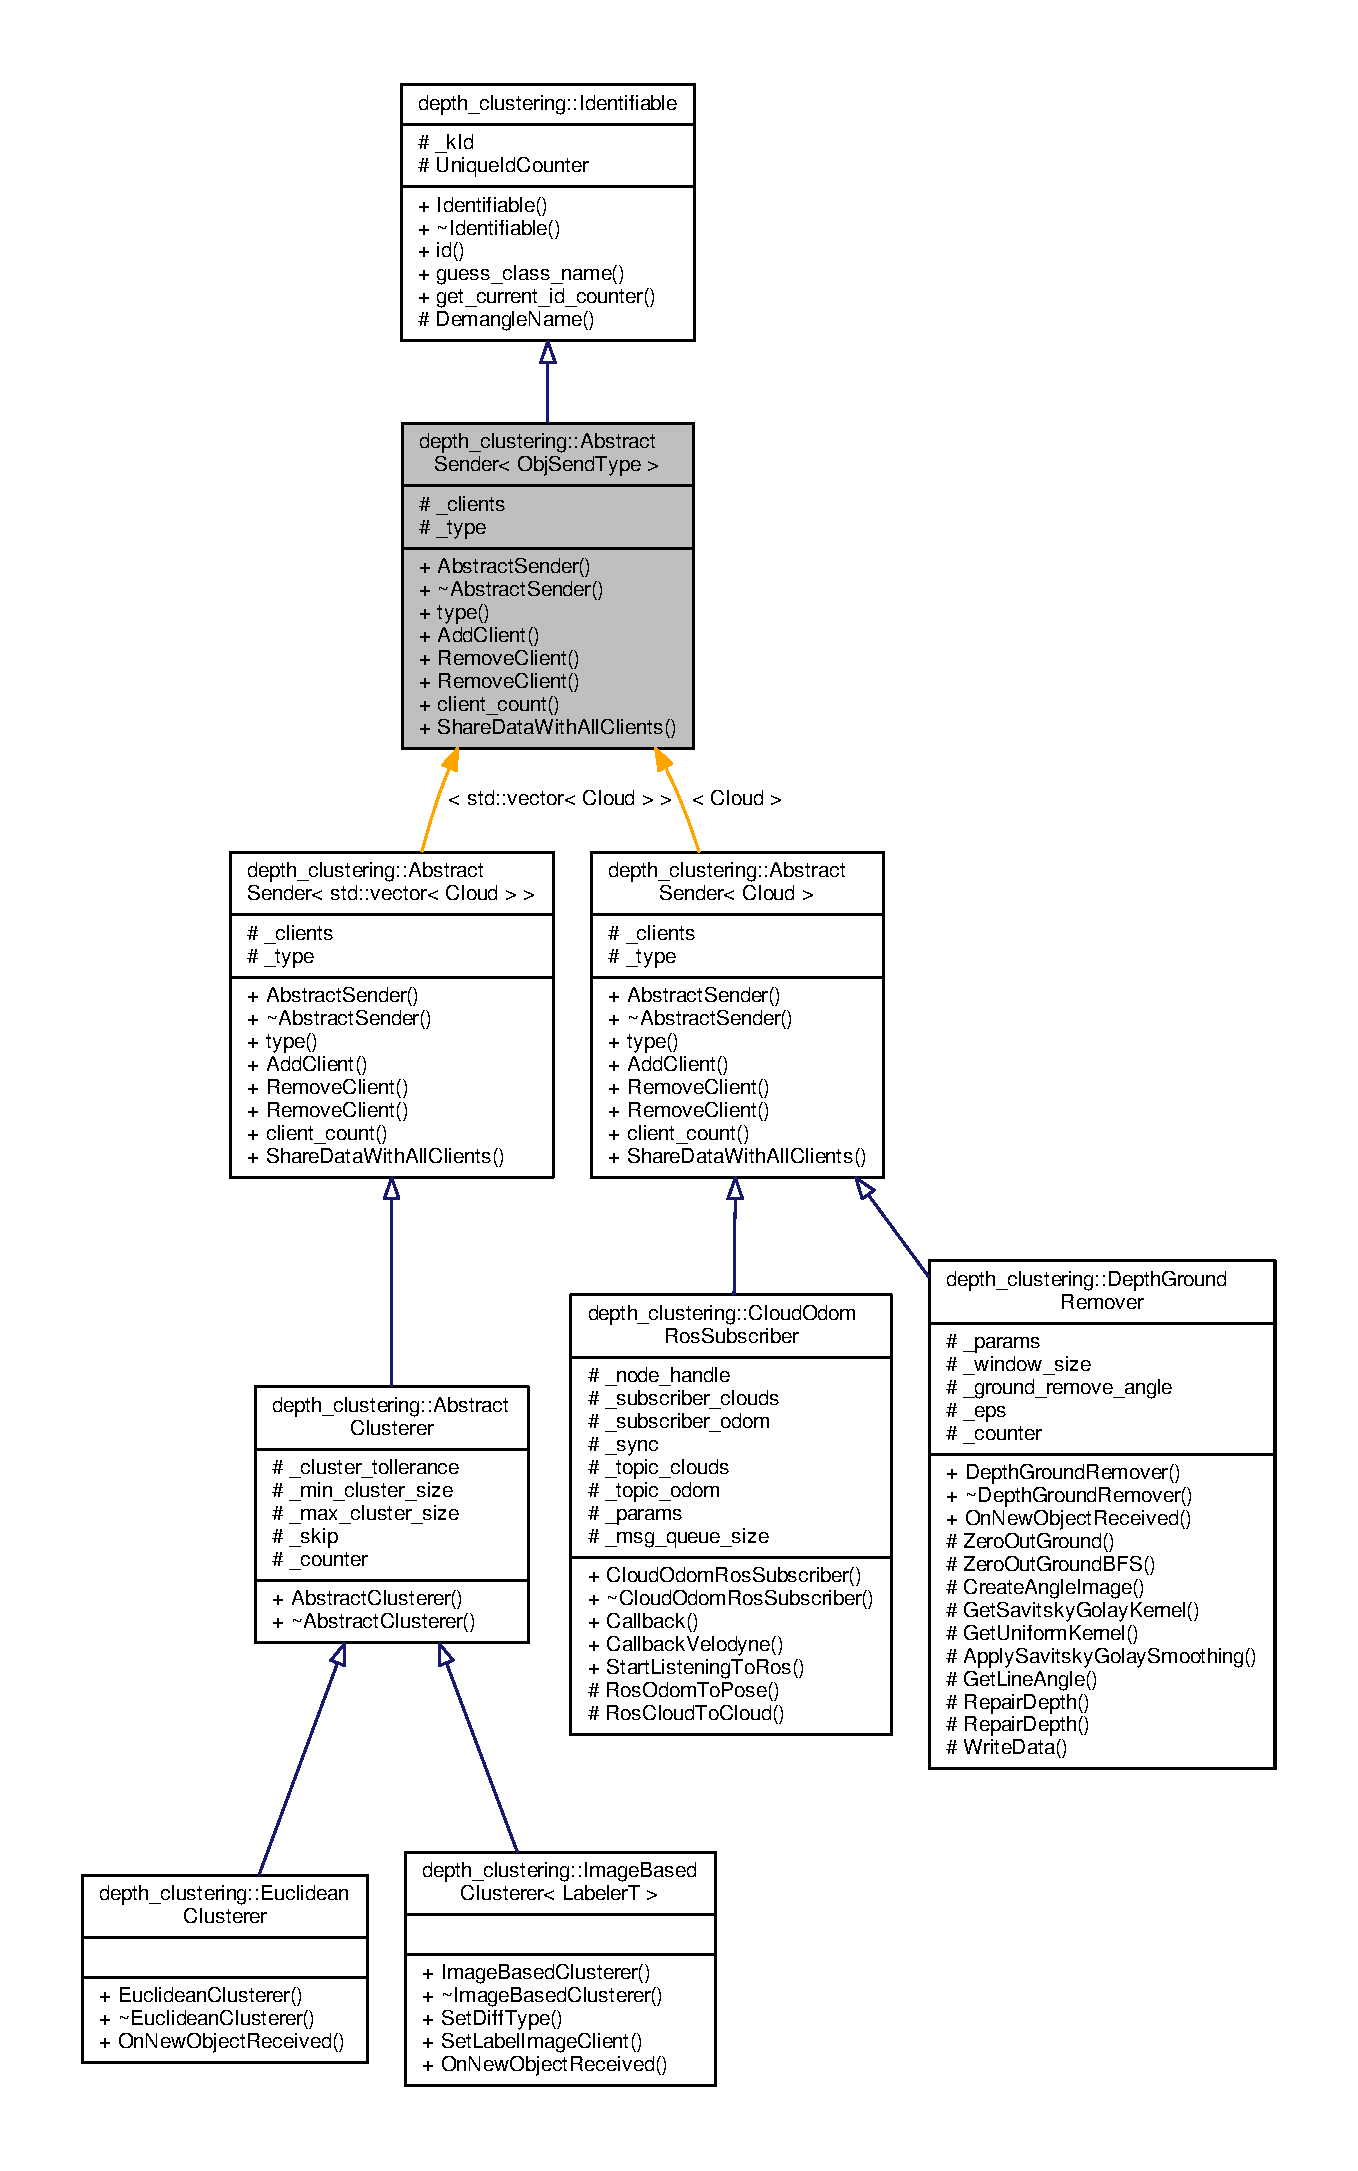
\includegraphics[height=550pt]{classdepth__clustering_1_1AbstractSender__inherit__graph}
\end{center}
\end{figure}


Collaboration diagram for depth\-\_\-clustering\-:\-:Abstract\-Sender$<$ Obj\-Send\-Type $>$\-:
\nopagebreak
\begin{figure}[H]
\begin{center}
\leavevmode
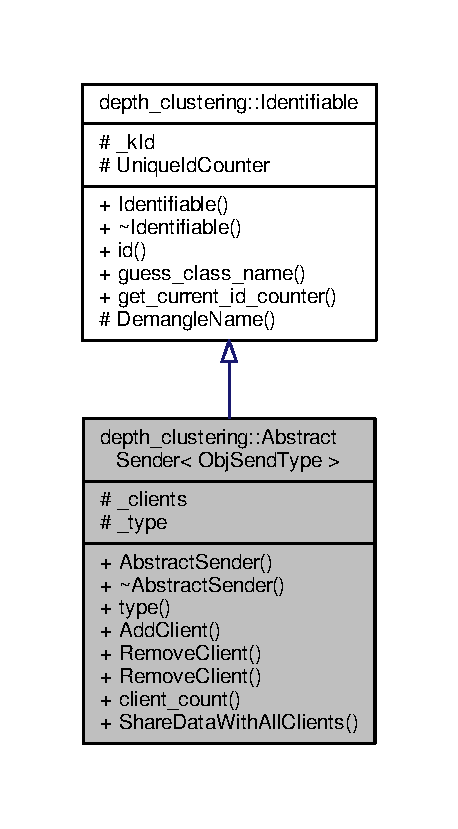
\includegraphics[width=220pt]{classdepth__clustering_1_1AbstractSender__coll__graph}
\end{center}
\end{figure}


\subsection{Member Function Documentation}
\hypertarget{classdepth__clustering_1_1AbstractSender_aca33c29cca1916fb0a3edd9024a49b51}{\index{depth\-\_\-clustering\-::\-Abstract\-Sender@{depth\-\_\-clustering\-::\-Abstract\-Sender}!Add\-Client@{Add\-Client}}
\index{Add\-Client@{Add\-Client}!depth_clustering::AbstractSender@{depth\-\_\-clustering\-::\-Abstract\-Sender}}
\subsubsection[{Add\-Client}]{\setlength{\rightskip}{0pt plus 5cm}template$<$class Obj\-Send\-Type$>$ void {\bf depth\-\_\-clustering\-::\-Abstract\-Sender}$<$ Obj\-Send\-Type $>$\-::Add\-Client (
\begin{DoxyParamCaption}
\item[{{\bf Abstract\-Client}$<$ Obj\-Send\-Type $>$ $\ast$}]{client}
\end{DoxyParamCaption}
)\hspace{0.3cm}{\ttfamily [inline]}}}\label{classdepth__clustering_1_1AbstractSender_aca33c29cca1916fb0a3edd9024a49b51}


Adds a client. 


\begin{DoxyParams}{Parameters}
{\em client} & The client to receive the processed data \\
\hline
\end{DoxyParams}
\hypertarget{classdepth__clustering_1_1AbstractSender_a957331eb41f11208bbe6174895c11bf2}{\index{depth\-\_\-clustering\-::\-Abstract\-Sender@{depth\-\_\-clustering\-::\-Abstract\-Sender}!client\-\_\-count@{client\-\_\-count}}
\index{client\-\_\-count@{client\-\_\-count}!depth_clustering::AbstractSender@{depth\-\_\-clustering\-::\-Abstract\-Sender}}
\subsubsection[{client\-\_\-count}]{\setlength{\rightskip}{0pt plus 5cm}template$<$class Obj\-Send\-Type$>$ size\-\_\-t {\bf depth\-\_\-clustering\-::\-Abstract\-Sender}$<$ Obj\-Send\-Type $>$\-::client\-\_\-count (
\begin{DoxyParamCaption}
{}
\end{DoxyParamCaption}
)\hspace{0.3cm}{\ttfamily [inline]}}}\label{classdepth__clustering_1_1AbstractSender_a957331eb41f11208bbe6174895c11bf2}


Get number of clients currently subscribed. 

\begin{DoxyReturn}{Returns}
Current number of Clients 
\end{DoxyReturn}
\hypertarget{classdepth__clustering_1_1AbstractSender_a0c33c98abe8fa71a86f02af95b1c71c1}{\index{depth\-\_\-clustering\-::\-Abstract\-Sender@{depth\-\_\-clustering\-::\-Abstract\-Sender}!Remove\-Client@{Remove\-Client}}
\index{Remove\-Client@{Remove\-Client}!depth_clustering::AbstractSender@{depth\-\_\-clustering\-::\-Abstract\-Sender}}
\subsubsection[{Remove\-Client}]{\setlength{\rightskip}{0pt plus 5cm}template$<$class Obj\-Send\-Type$>$ void {\bf depth\-\_\-clustering\-::\-Abstract\-Sender}$<$ Obj\-Send\-Type $>$\-::Remove\-Client (
\begin{DoxyParamCaption}
\item[{int}]{id}
\end{DoxyParamCaption}
)\hspace{0.3cm}{\ttfamily [inline]}}}\label{classdepth__clustering_1_1AbstractSender_a0c33c98abe8fa71a86f02af95b1c71c1}


Removes a client. 


\begin{DoxyParams}[1]{Parameters}
\mbox{\tt in}  & {\em id} & The identifier of the client to remove \\
\hline
\end{DoxyParams}
\hypertarget{classdepth__clustering_1_1AbstractSender_a147752e5ab7ca15da9c8d8e60575390b}{\index{depth\-\_\-clustering\-::\-Abstract\-Sender@{depth\-\_\-clustering\-::\-Abstract\-Sender}!Share\-Data\-With\-All\-Clients@{Share\-Data\-With\-All\-Clients}}
\index{Share\-Data\-With\-All\-Clients@{Share\-Data\-With\-All\-Clients}!depth_clustering::AbstractSender@{depth\-\_\-clustering\-::\-Abstract\-Sender}}
\subsubsection[{Share\-Data\-With\-All\-Clients}]{\setlength{\rightskip}{0pt plus 5cm}template$<$class Obj\-Send\-Type$>$ void {\bf depth\-\_\-clustering\-::\-Abstract\-Sender}$<$ Obj\-Send\-Type $>$\-::Share\-Data\-With\-All\-Clients (
\begin{DoxyParamCaption}
\item[{const Obj\-Send\-Type \&}]{obj, }
\item[{int}]{id = {\ttfamily -\/1}}
\end{DoxyParamCaption}
)\hspace{0.3cm}{\ttfamily [inline]}}}\label{classdepth__clustering_1_1AbstractSender_a147752e5ab7ca15da9c8d8e60575390b}


Shares data with everyone who listens to it. 


\begin{DoxyParams}[1]{Parameters}
\mbox{\tt in}  & {\em obj} & Object to share \\
\hline
\mbox{\tt in}  & {\em id} & Id, by default this-\/$>$\hyperlink{classdepth__clustering_1_1Identifiable_a020b49a5102a2ef0eec7b9e74add7669}{id()} \\
\hline
\end{DoxyParams}
\hypertarget{classdepth__clustering_1_1AbstractSender_ad9da304185f766eb4b0035d6610caa49}{\index{depth\-\_\-clustering\-::\-Abstract\-Sender@{depth\-\_\-clustering\-::\-Abstract\-Sender}!type@{type}}
\index{type@{type}!depth_clustering::AbstractSender@{depth\-\_\-clustering\-::\-Abstract\-Sender}}
\subsubsection[{type}]{\setlength{\rightskip}{0pt plus 5cm}template$<$class Obj\-Send\-Type$>$ const char$\ast$ {\bf depth\-\_\-clustering\-::\-Abstract\-Sender}$<$ Obj\-Send\-Type $>$\-::type (
\begin{DoxyParamCaption}
{}
\end{DoxyParamCaption}
) const\hspace{0.3cm}{\ttfamily [inline]}}}\label{classdepth__clustering_1_1AbstractSender_ad9da304185f766eb4b0035d6610caa49}


Gets type of sender as string. 

\begin{DoxyReturn}{Returns}
Type as string 
\end{DoxyReturn}


Here is the caller graph for this function\-:
\nopagebreak
\begin{figure}[H]
\begin{center}
\leavevmode
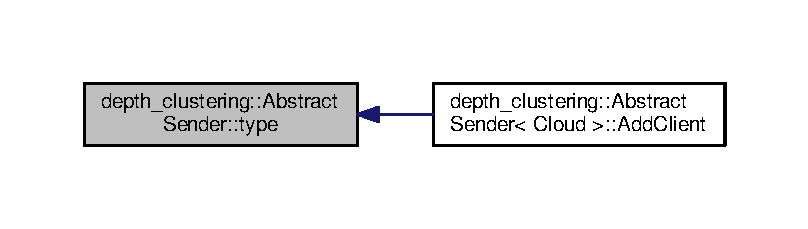
\includegraphics[width=350pt]{classdepth__clustering_1_1AbstractSender_ad9da304185f766eb4b0035d6610caa49_icgraph}
\end{center}
\end{figure}




The documentation for this class was generated from the following file\-:\begin{DoxyCompactItemize}
\item 
/home/hadoop/chy/depth\-\_\-clustering-\/master234/src/communication/abstract\-\_\-sender.\-h\end{DoxyCompactItemize}

\hypertarget{classdepth__clustering_1_1AngleDiff}{\section{depth\-\_\-clustering\-:\-:Angle\-Diff Class Reference}
\label{classdepth__clustering_1_1AngleDiff}\index{depth\-\_\-clustering\-::\-Angle\-Diff@{depth\-\_\-clustering\-::\-Angle\-Diff}}
}


Class for angle difference.  




{\ttfamily \#include $<$angle\-\_\-diff.\-h$>$}

\subsection*{Public Member Functions}
\begin{DoxyCompactItemize}
\item 
\hyperlink{classdepth__clustering_1_1AngleDiff_a40371150bff3a10dd8ce40788b9bd160}{Angle\-Diff} (const cv\-::\-Mat $\ast$source\-\_\-image, const \hyperlink{classdepth__clustering_1_1ProjectionParams}{Projection\-Params} $\ast$params)
\begin{DoxyCompactList}\small\item\em Precompute the angles to avoid losing time on that. \end{DoxyCompactList}\item 
float \hyperlink{classdepth__clustering_1_1AngleDiff_ac9bd0ec61ff0b213fd19235dc171c1c2}{Diff\-At} (const \hyperlink{structdepth__clustering_1_1PixelCoord}{Pixel\-Coord} \&from, const \hyperlink{structdepth__clustering_1_1PixelCoord}{Pixel\-Coord} \&to) const override
\begin{DoxyCompactList}\small\item\em Compute angle-\/based difference. See paper for details. \end{DoxyCompactList}\item 
\hypertarget{classdepth__clustering_1_1AngleDiff_ac65e8f42b1f2ac82db14ebe188c004a2}{bool \hyperlink{classdepth__clustering_1_1AngleDiff_ac65e8f42b1f2ac82db14ebe188c004a2}{Satisfies\-Threshold} (float angle, float threshold) const override}\label{classdepth__clustering_1_1AngleDiff_ac65e8f42b1f2ac82db14ebe188c004a2}

\begin{DoxyCompactList}\small\item\em Threshold is satisfied if angle is B\-I\-G\-G\-E\-R than threshold. \end{DoxyCompactList}\item 
cv\-::\-Mat \hyperlink{classdepth__clustering_1_1AngleDiff_a462e4aadd35ca06e9b061d08c9787074}{Visualize} () const override
\begin{DoxyCompactList}\small\item\em Visualize $\beta$ angles as a {\ttfamily cv\-::\-Mat} color image. \end{DoxyCompactList}\end{DoxyCompactItemize}
\subsection*{Additional Inherited Members}


\subsection{Detailed Description}
Class for angle difference. 

Inheritance diagram for depth\-\_\-clustering\-:\-:Angle\-Diff\-:
\nopagebreak
\begin{figure}[H]
\begin{center}
\leavevmode
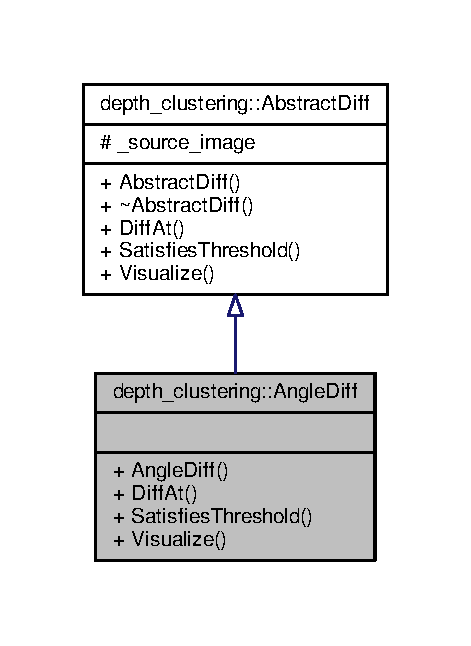
\includegraphics[width=226pt]{classdepth__clustering_1_1AngleDiff__inherit__graph}
\end{center}
\end{figure}


Collaboration diagram for depth\-\_\-clustering\-:\-:Angle\-Diff\-:
\nopagebreak
\begin{figure}[H]
\begin{center}
\leavevmode
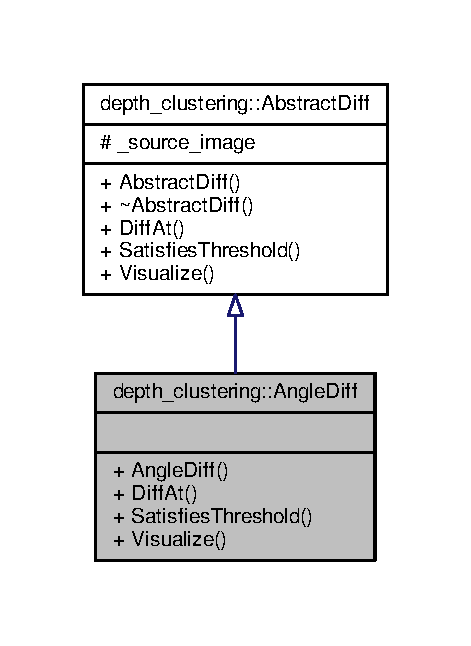
\includegraphics[width=226pt]{classdepth__clustering_1_1AngleDiff__coll__graph}
\end{center}
\end{figure}


\subsection{Constructor \& Destructor Documentation}
\hypertarget{classdepth__clustering_1_1AngleDiff_a40371150bff3a10dd8ce40788b9bd160}{\index{depth\-\_\-clustering\-::\-Angle\-Diff@{depth\-\_\-clustering\-::\-Angle\-Diff}!Angle\-Diff@{Angle\-Diff}}
\index{Angle\-Diff@{Angle\-Diff}!depth_clustering::AngleDiff@{depth\-\_\-clustering\-::\-Angle\-Diff}}
\subsubsection[{Angle\-Diff}]{\setlength{\rightskip}{0pt plus 5cm}depth\-\_\-clustering\-::\-Angle\-Diff\-::\-Angle\-Diff (
\begin{DoxyParamCaption}
\item[{const cv\-::\-Mat $\ast$}]{source\-\_\-image, }
\item[{const {\bf Projection\-Params} $\ast$}]{params}
\end{DoxyParamCaption}
)}}\label{classdepth__clustering_1_1AngleDiff_a40371150bff3a10dd8ce40788b9bd160}


Precompute the angles to avoid losing time on that. 


\begin{DoxyParams}[1]{Parameters}
\mbox{\tt in}  & {\em source\-\_\-image} & The source image \\
\hline
\mbox{\tt in}  & {\em params} & The projection parameters \\
\hline
\end{DoxyParams}


\subsection{Member Function Documentation}
\hypertarget{classdepth__clustering_1_1AngleDiff_ac9bd0ec61ff0b213fd19235dc171c1c2}{\index{depth\-\_\-clustering\-::\-Angle\-Diff@{depth\-\_\-clustering\-::\-Angle\-Diff}!Diff\-At@{Diff\-At}}
\index{Diff\-At@{Diff\-At}!depth_clustering::AngleDiff@{depth\-\_\-clustering\-::\-Angle\-Diff}}
\subsubsection[{Diff\-At}]{\setlength{\rightskip}{0pt plus 5cm}float depth\-\_\-clustering\-::\-Angle\-Diff\-::\-Diff\-At (
\begin{DoxyParamCaption}
\item[{const {\bf Pixel\-Coord} \&}]{from, }
\item[{const {\bf Pixel\-Coord} \&}]{to}
\end{DoxyParamCaption}
) const\hspace{0.3cm}{\ttfamily [override]}, {\ttfamily [virtual]}}}\label{classdepth__clustering_1_1AngleDiff_ac9bd0ec61ff0b213fd19235dc171c1c2}


Compute angle-\/based difference. See paper for details. 


\begin{DoxyParams}[1]{Parameters}
\mbox{\tt in}  & {\em from} & Pixel from which to compute difference \\
\hline
\mbox{\tt in}  & {\em to} & Pixel to which to compute difference\\
\hline
\end{DoxyParams}
\begin{DoxyReturn}{Returns}
Angle difference between the values 
\end{DoxyReturn}


Implements \hyperlink{classdepth__clustering_1_1AbstractDiff_a06ba188d8d83d0e4bad66c833656c26d}{depth\-\_\-clustering\-::\-Abstract\-Diff}.

\hypertarget{classdepth__clustering_1_1AngleDiff_a462e4aadd35ca06e9b061d08c9787074}{\index{depth\-\_\-clustering\-::\-Angle\-Diff@{depth\-\_\-clustering\-::\-Angle\-Diff}!Visualize@{Visualize}}
\index{Visualize@{Visualize}!depth_clustering::AngleDiff@{depth\-\_\-clustering\-::\-Angle\-Diff}}
\subsubsection[{Visualize}]{\setlength{\rightskip}{0pt plus 5cm}cv\-::\-Mat depth\-\_\-clustering\-::\-Angle\-Diff\-::\-Visualize (
\begin{DoxyParamCaption}
{}
\end{DoxyParamCaption}
) const\hspace{0.3cm}{\ttfamily [inline]}, {\ttfamily [override]}, {\ttfamily [virtual]}}}\label{classdepth__clustering_1_1AngleDiff_a462e4aadd35ca06e9b061d08c9787074}


Visualize $\beta$ angles as a {\ttfamily cv\-::\-Mat} color image. 

\begin{DoxyReturn}{Returns}
{\ttfamily cv\-::\-Mat} color image with red channel showing $\beta$ angles in row direction and green channel in col direction. 
\end{DoxyReturn}


Reimplemented from \hyperlink{classdepth__clustering_1_1AbstractDiff_a5500c82f3e6800922ba6fc6c22c6d0bf}{depth\-\_\-clustering\-::\-Abstract\-Diff}.



The documentation for this class was generated from the following files\-:\begin{DoxyCompactItemize}
\item 
/home/hadoop/chy/depth\-\_\-clustering-\/master234/src/image\-\_\-labelers/diff\-\_\-helpers/angle\-\_\-diff.\-h\item 
/home/hadoop/chy/depth\-\_\-clustering-\/master234/src/image\-\_\-labelers/diff\-\_\-helpers/angle\-\_\-diff.\-cpp\end{DoxyCompactItemize}

\hypertarget{classdepth__clustering_1_1AngleDiffPrecomputed}{\section{depth\-\_\-clustering\-:\-:Angle\-Diff\-Precomputed Class Reference}
\label{classdepth__clustering_1_1AngleDiffPrecomputed}\index{depth\-\_\-clustering\-::\-Angle\-Diff\-Precomputed@{depth\-\_\-clustering\-::\-Angle\-Diff\-Precomputed}}
}


Class for angle difference.  




{\ttfamily \#include $<$angle\-\_\-diff.\-h$>$}

\subsection*{Public Member Functions}
\begin{DoxyCompactItemize}
\item 
\hyperlink{classdepth__clustering_1_1AngleDiffPrecomputed_a0cd5a0071d191d6a4f3594a789777ff3}{Angle\-Diff\-Precomputed} (const cv\-::\-Mat $\ast$source\-\_\-image, const \hyperlink{classdepth__clustering_1_1ProjectionParams}{Projection\-Params} $\ast$params)
\begin{DoxyCompactList}\small\item\em Precompute the angles to avoid losing time on that. \end{DoxyCompactList}\item 
float \hyperlink{classdepth__clustering_1_1AngleDiffPrecomputed_ae15bb5fc9488ae2b26c77665931b8626}{Diff\-At} (const \hyperlink{structdepth__clustering_1_1PixelCoord}{Pixel\-Coord} \&from, const \hyperlink{structdepth__clustering_1_1PixelCoord}{Pixel\-Coord} \&to) const override
\begin{DoxyCompactList}\small\item\em Compute angle-\/based difference. See paper for details. Only one of the following situations is possible\-: \end{DoxyCompactList}\item 
\hypertarget{classdepth__clustering_1_1AngleDiffPrecomputed_a28a32c0cb0405163fe237909fe5f6c0c}{bool \hyperlink{classdepth__clustering_1_1AngleDiffPrecomputed_a28a32c0cb0405163fe237909fe5f6c0c}{Satisfies\-Threshold} (float angle, float threshold) const override}\label{classdepth__clustering_1_1AngleDiffPrecomputed_a28a32c0cb0405163fe237909fe5f6c0c}

\begin{DoxyCompactList}\small\item\em Threshold is satisfied if angle is B\-I\-G\-G\-E\-R than threshold. \end{DoxyCompactList}\item 
cv\-::\-Mat \hyperlink{classdepth__clustering_1_1AngleDiffPrecomputed_a35da8cd9455b3485acfd5da203ecaafb}{Visualize} () const 
\begin{DoxyCompactList}\small\item\em Visualize $\beta$ angles as a {\ttfamily cv\-::\-Mat} color image. \end{DoxyCompactList}\end{DoxyCompactItemize}
\subsection*{Protected Member Functions}
\begin{DoxyCompactItemize}
\item 
\hypertarget{classdepth__clustering_1_1AngleDiffPrecomputed_a8f333b5196e9dcaa7923f82d362c7281}{void \hyperlink{classdepth__clustering_1_1AngleDiffPrecomputed_a8f333b5196e9dcaa7923f82d362c7281}{Pre\-Compute\-Alpha\-Vecs} ()}\label{classdepth__clustering_1_1AngleDiffPrecomputed_a8f333b5196e9dcaa7923f82d362c7281}

\begin{DoxyCompactList}\small\item\em Pre-\/compute values for angles for all cols and rows. \end{DoxyCompactList}\item 
void \hyperlink{classdepth__clustering_1_1AngleDiffPrecomputed_aeb86ee61c6e8fc1b5b554368b1f5fa27}{Pre\-Compute\-Beta\-Angles} ()
\begin{DoxyCompactList}\small\item\em Precompute all $\beta$ angles for the image. It generates two matrices for row-\/wise and col-\/wise angles. See picture for illustration. The squares store values of angles between pixels with computation direction shown by arrows. Note that the columns matrix wraps around, i.\-e. the last element stores the difference in angles between the last pixel of the original image and the first one. \end{DoxyCompactList}\item 
float \hyperlink{classdepth__clustering_1_1AngleDiffPrecomputed_a717fd502674b9a61d29382e5a2cfbaee}{Get\-Beta} (float alpha, float current\-\_\-depth, float neighbor\-\_\-depth) const 
\begin{DoxyCompactList}\small\item\em Compute the angle $\beta$ of incline of the line spawned by two given beams. \end{DoxyCompactList}\end{DoxyCompactItemize}
\subsection*{Protected Attributes}
\begin{DoxyCompactItemize}
\item 
\hypertarget{classdepth__clustering_1_1AngleDiffPrecomputed_ac37e01df194d9063b7e7bd1f7b7aa6a4}{const \hyperlink{classdepth__clustering_1_1ProjectionParams}{Projection\-Params} $\ast$ {\bfseries \-\_\-params} = nullptr}\label{classdepth__clustering_1_1AngleDiffPrecomputed_ac37e01df194d9063b7e7bd1f7b7aa6a4}

\item 
\hypertarget{classdepth__clustering_1_1AngleDiffPrecomputed_a2ba86b3ed5f12c2a7e2e8beef81bd88d}{std\-::vector$<$ float $>$ {\bfseries \-\_\-row\-\_\-alphas}}\label{classdepth__clustering_1_1AngleDiffPrecomputed_a2ba86b3ed5f12c2a7e2e8beef81bd88d}

\item 
\hypertarget{classdepth__clustering_1_1AngleDiffPrecomputed_a90f6e3fd2f4b585c2cd03809f3818ee9}{std\-::vector$<$ float $>$ {\bfseries \-\_\-col\-\_\-alphas}}\label{classdepth__clustering_1_1AngleDiffPrecomputed_a90f6e3fd2f4b585c2cd03809f3818ee9}

\item 
\hypertarget{classdepth__clustering_1_1AngleDiffPrecomputed_a2df8751352e4621cb69743801e151b75}{cv\-::\-Mat {\bfseries \-\_\-beta\-\_\-rows}}\label{classdepth__clustering_1_1AngleDiffPrecomputed_a2df8751352e4621cb69743801e151b75}

\item 
\hypertarget{classdepth__clustering_1_1AngleDiffPrecomputed_ae7faa81ea82d0ff9f75f8a1e63659ced}{cv\-::\-Mat {\bfseries \-\_\-beta\-\_\-cols}}\label{classdepth__clustering_1_1AngleDiffPrecomputed_ae7faa81ea82d0ff9f75f8a1e63659ced}

\end{DoxyCompactItemize}


\subsection{Detailed Description}
Class for angle difference. 

Inheritance diagram for depth\-\_\-clustering\-:\-:Angle\-Diff\-Precomputed\-:
\nopagebreak
\begin{figure}[H]
\begin{center}
\leavevmode
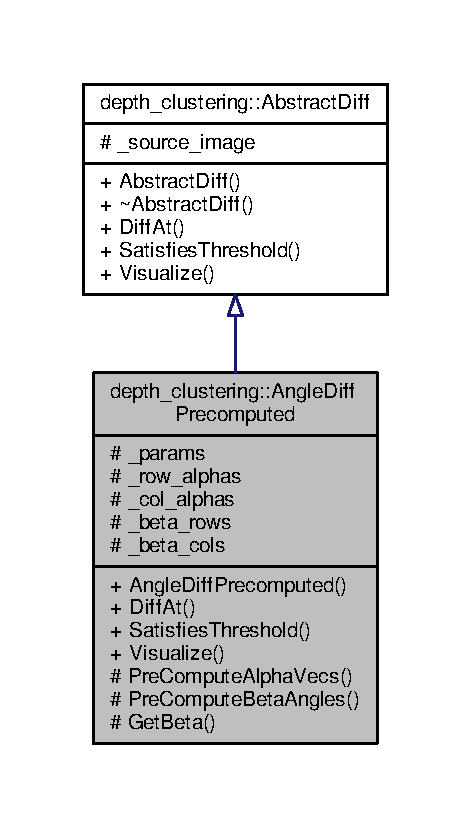
\includegraphics[width=226pt]{classdepth__clustering_1_1AngleDiffPrecomputed__inherit__graph}
\end{center}
\end{figure}


Collaboration diagram for depth\-\_\-clustering\-:\-:Angle\-Diff\-Precomputed\-:
\nopagebreak
\begin{figure}[H]
\begin{center}
\leavevmode
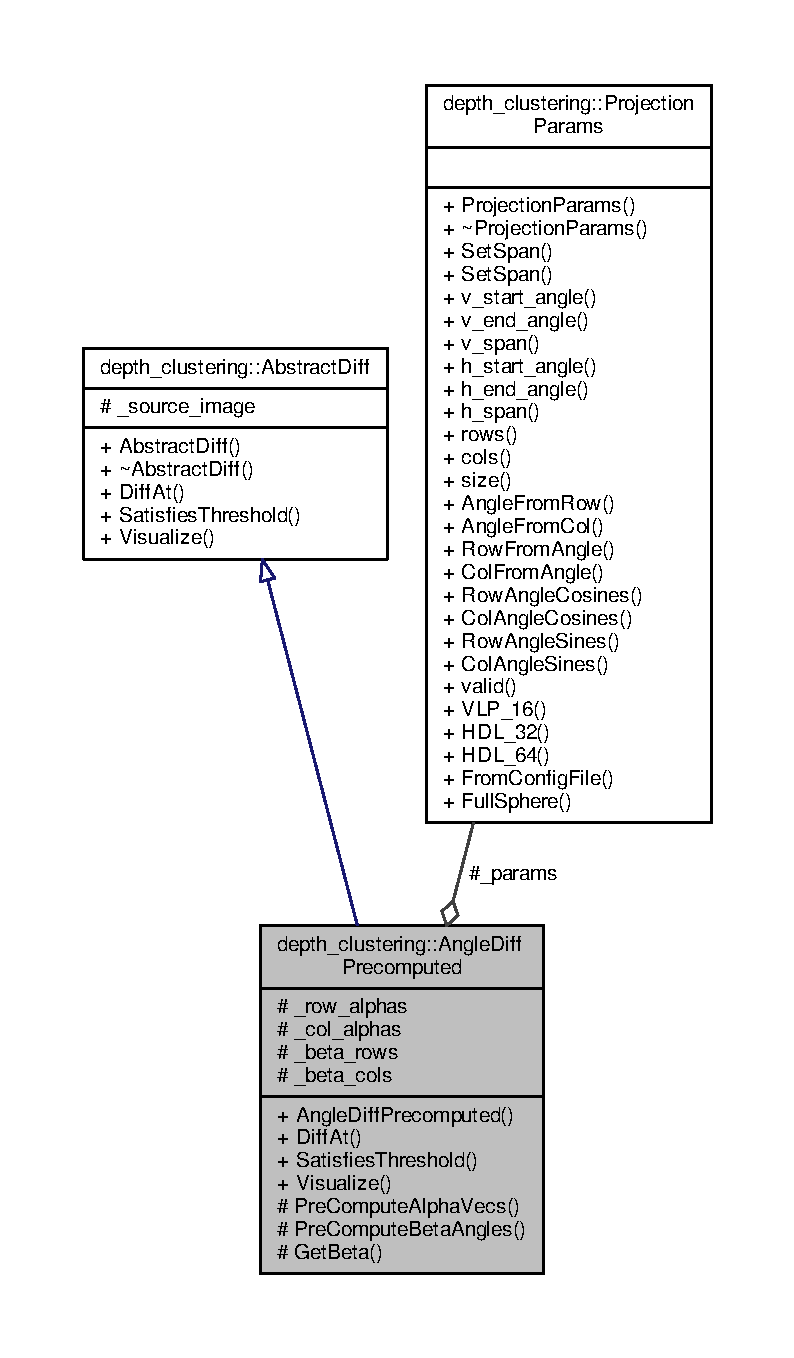
\includegraphics[height=550pt]{classdepth__clustering_1_1AngleDiffPrecomputed__coll__graph}
\end{center}
\end{figure}


\subsection{Constructor \& Destructor Documentation}
\hypertarget{classdepth__clustering_1_1AngleDiffPrecomputed_a0cd5a0071d191d6a4f3594a789777ff3}{\index{depth\-\_\-clustering\-::\-Angle\-Diff\-Precomputed@{depth\-\_\-clustering\-::\-Angle\-Diff\-Precomputed}!Angle\-Diff\-Precomputed@{Angle\-Diff\-Precomputed}}
\index{Angle\-Diff\-Precomputed@{Angle\-Diff\-Precomputed}!depth_clustering::AngleDiffPrecomputed@{depth\-\_\-clustering\-::\-Angle\-Diff\-Precomputed}}
\subsubsection[{Angle\-Diff\-Precomputed}]{\setlength{\rightskip}{0pt plus 5cm}depth\-\_\-clustering\-::\-Angle\-Diff\-Precomputed\-::\-Angle\-Diff\-Precomputed (
\begin{DoxyParamCaption}
\item[{const cv\-::\-Mat $\ast$}]{source\-\_\-image, }
\item[{const {\bf Projection\-Params} $\ast$}]{params}
\end{DoxyParamCaption}
)}}\label{classdepth__clustering_1_1AngleDiffPrecomputed_a0cd5a0071d191d6a4f3594a789777ff3}


Precompute the angles to avoid losing time on that. 


\begin{DoxyParams}[1]{Parameters}
\mbox{\tt in}  & {\em source\-\_\-image} & The source image \\
\hline
\mbox{\tt in}  & {\em params} & The projection parameters \\
\hline
\end{DoxyParams}


\subsection{Member Function Documentation}
\hypertarget{classdepth__clustering_1_1AngleDiffPrecomputed_ae15bb5fc9488ae2b26c77665931b8626}{\index{depth\-\_\-clustering\-::\-Angle\-Diff\-Precomputed@{depth\-\_\-clustering\-::\-Angle\-Diff\-Precomputed}!Diff\-At@{Diff\-At}}
\index{Diff\-At@{Diff\-At}!depth_clustering::AngleDiffPrecomputed@{depth\-\_\-clustering\-::\-Angle\-Diff\-Precomputed}}
\subsubsection[{Diff\-At}]{\setlength{\rightskip}{0pt plus 5cm}float depth\-\_\-clustering\-::\-Angle\-Diff\-Precomputed\-::\-Diff\-At (
\begin{DoxyParamCaption}
\item[{const {\bf Pixel\-Coord} \&}]{from, }
\item[{const {\bf Pixel\-Coord} \&}]{to}
\end{DoxyParamCaption}
) const\hspace{0.3cm}{\ttfamily [override]}, {\ttfamily [virtual]}}}\label{classdepth__clustering_1_1AngleDiffPrecomputed_ae15bb5fc9488ae2b26c77665931b8626}


Compute angle-\/based difference. See paper for details. Only one of the following situations is possible\-: 


\begin{DoxyItemize}
\item from.\-row $>$ to.\-row
\item from.\-row $<$ to.\-row
\item from.\-col $>$ to.\-col
\item from.\-col $<$ to.\-col
\end{DoxyItemize}


\begin{DoxyParams}[1]{Parameters}
\mbox{\tt in}  & {\em from} & Pixel from which to compute difference \\
\hline
\mbox{\tt in}  & {\em to} & Pixel to which to compute difference\\
\hline
\end{DoxyParams}
\begin{DoxyReturn}{Returns}
Angle difference between the values 
\end{DoxyReturn}
If one of rows is biggest possible -\/ use it. Otherwise use {\ttfamily std\-::min(from.\-row, to.\-row)}.

If one of cols is biggest possible -\/ use it. Otherwise use {\ttfamily std\-::min(from.\-col, to.\-col)}. 

Implements \hyperlink{classdepth__clustering_1_1AbstractDiff_a06ba188d8d83d0e4bad66c833656c26d}{depth\-\_\-clustering\-::\-Abstract\-Diff}.

\hypertarget{classdepth__clustering_1_1AngleDiffPrecomputed_a717fd502674b9a61d29382e5a2cfbaee}{\index{depth\-\_\-clustering\-::\-Angle\-Diff\-Precomputed@{depth\-\_\-clustering\-::\-Angle\-Diff\-Precomputed}!Get\-Beta@{Get\-Beta}}
\index{Get\-Beta@{Get\-Beta}!depth_clustering::AngleDiffPrecomputed@{depth\-\_\-clustering\-::\-Angle\-Diff\-Precomputed}}
\subsubsection[{Get\-Beta}]{\setlength{\rightskip}{0pt plus 5cm}float depth\-\_\-clustering\-::\-Angle\-Diff\-Precomputed\-::\-Get\-Beta (
\begin{DoxyParamCaption}
\item[{float}]{alpha, }
\item[{float}]{current\-\_\-depth, }
\item[{float}]{neighbor\-\_\-depth}
\end{DoxyParamCaption}
) const\hspace{0.3cm}{\ttfamily [protected]}}}\label{classdepth__clustering_1_1AngleDiffPrecomputed_a717fd502674b9a61d29382e5a2cfbaee}


Compute the angle $\beta$ of incline of the line spawned by two given beams. 


\begin{DoxyParams}[1]{Parameters}
\mbox{\tt in}  & {\em alpha} & The angle $\alpha$ between the beams. \\
\hline
\mbox{\tt in}  & {\em current\-\_\-depth} & The reading of the first beam in meters. \\
\hline
\mbox{\tt in}  & {\em neighbor\-\_\-depth} & The reading of the second beam in meters.\\
\hline
\end{DoxyParams}
\begin{DoxyReturn}{Returns}
The angle of incidence of the line spawned by endpoints of two given beams. 
\end{DoxyReturn}


Here is the caller graph for this function\-:
\nopagebreak
\begin{figure}[H]
\begin{center}
\leavevmode
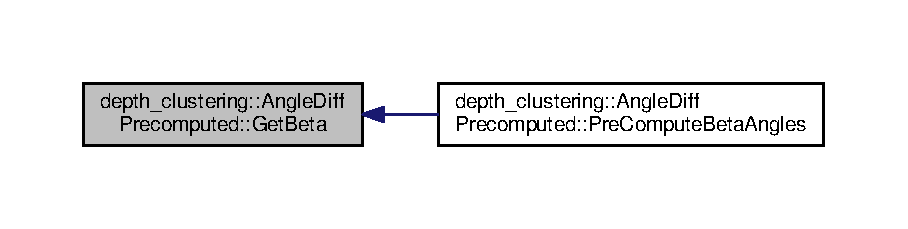
\includegraphics[width=350pt]{classdepth__clustering_1_1AngleDiffPrecomputed_a717fd502674b9a61d29382e5a2cfbaee_icgraph}
\end{center}
\end{figure}


\hypertarget{classdepth__clustering_1_1AngleDiffPrecomputed_aeb86ee61c6e8fc1b5b554368b1f5fa27}{\index{depth\-\_\-clustering\-::\-Angle\-Diff\-Precomputed@{depth\-\_\-clustering\-::\-Angle\-Diff\-Precomputed}!Pre\-Compute\-Beta\-Angles@{Pre\-Compute\-Beta\-Angles}}
\index{Pre\-Compute\-Beta\-Angles@{Pre\-Compute\-Beta\-Angles}!depth_clustering::AngleDiffPrecomputed@{depth\-\_\-clustering\-::\-Angle\-Diff\-Precomputed}}
\subsubsection[{Pre\-Compute\-Beta\-Angles}]{\setlength{\rightskip}{0pt plus 5cm}void depth\-\_\-clustering\-::\-Angle\-Diff\-Precomputed\-::\-Pre\-Compute\-Beta\-Angles (
\begin{DoxyParamCaption}
{}
\end{DoxyParamCaption}
)\hspace{0.3cm}{\ttfamily [protected]}}}\label{classdepth__clustering_1_1AngleDiffPrecomputed_aeb86ee61c6e8fc1b5b554368b1f5fa27}


Precompute all $\beta$ angles for the image. It generates two matrices for row-\/wise and col-\/wise angles. See picture for illustration. The squares store values of angles between pixels with computation direction shown by arrows. Note that the columns matrix wraps around, i.\-e. the last element stores the difference in angles between the last pixel of the original image and the first one. 

 

Here is the call graph for this function\-:
\nopagebreak
\begin{figure}[H]
\begin{center}
\leavevmode
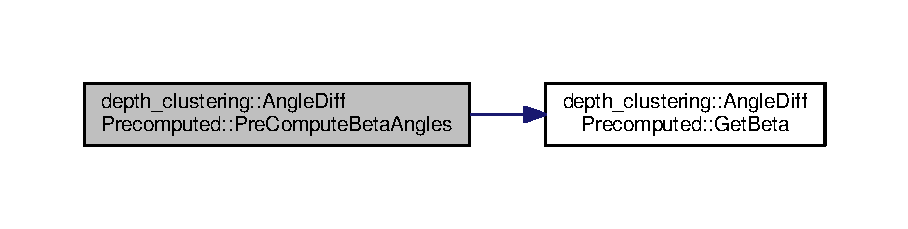
\includegraphics[width=350pt]{classdepth__clustering_1_1AngleDiffPrecomputed_aeb86ee61c6e8fc1b5b554368b1f5fa27_cgraph}
\end{center}
\end{figure}


\hypertarget{classdepth__clustering_1_1AngleDiffPrecomputed_a35da8cd9455b3485acfd5da203ecaafb}{\index{depth\-\_\-clustering\-::\-Angle\-Diff\-Precomputed@{depth\-\_\-clustering\-::\-Angle\-Diff\-Precomputed}!Visualize@{Visualize}}
\index{Visualize@{Visualize}!depth_clustering::AngleDiffPrecomputed@{depth\-\_\-clustering\-::\-Angle\-Diff\-Precomputed}}
\subsubsection[{Visualize}]{\setlength{\rightskip}{0pt plus 5cm}cv\-::\-Mat depth\-\_\-clustering\-::\-Angle\-Diff\-Precomputed\-::\-Visualize (
\begin{DoxyParamCaption}
{}
\end{DoxyParamCaption}
) const\hspace{0.3cm}{\ttfamily [virtual]}}}\label{classdepth__clustering_1_1AngleDiffPrecomputed_a35da8cd9455b3485acfd5da203ecaafb}


Visualize $\beta$ angles as a {\ttfamily cv\-::\-Mat} color image. 

\begin{DoxyReturn}{Returns}
{\ttfamily cv\-::\-Mat} color image with red channel showing $\beta$ angles in row direction and green channel in col direction. 
\end{DoxyReturn}


Reimplemented from \hyperlink{classdepth__clustering_1_1AbstractDiff_a5500c82f3e6800922ba6fc6c22c6d0bf}{depth\-\_\-clustering\-::\-Abstract\-Diff}.



The documentation for this class was generated from the following files\-:\begin{DoxyCompactItemize}
\item 
/home/hadoop/chy/depth\-\_\-clustering-\/master234/src/image\-\_\-labelers/diff\-\_\-helpers/angle\-\_\-diff.\-h\item 
/home/hadoop/chy/depth\-\_\-clustering-\/master234/src/image\-\_\-labelers/diff\-\_\-helpers/angle\-\_\-diff.\-cpp\end{DoxyCompactItemize}

\hypertarget{classdepth__clustering_1_1Cloud}{\section{depth\-\_\-clustering\-:\-:Cloud Class Reference}
\label{classdepth__clustering_1_1Cloud}\index{depth\-\_\-clustering\-::\-Cloud@{depth\-\_\-clustering\-::\-Cloud}}
}


A class that stores a vector of Rich\-Points.  




{\ttfamily \#include $<$cloud.\-h$>$}

\subsection*{Public Types}
\begin{DoxyCompactItemize}
\item 
\hypertarget{classdepth__clustering_1_1Cloud_a6357719aeeb7c05cbd4a375f63526ba1}{using {\bfseries Ptr} = shared\-\_\-ptr$<$ \hyperlink{classdepth__clustering_1_1Cloud}{Cloud} $>$}\label{classdepth__clustering_1_1Cloud_a6357719aeeb7c05cbd4a375f63526ba1}

\item 
\hypertarget{classdepth__clustering_1_1Cloud_ae8ba86a4493a06d04e25cba4e97b9787}{using {\bfseries Const\-Ptr} = shared\-\_\-ptr$<$ const \hyperlink{classdepth__clustering_1_1Cloud}{Cloud} $>$}\label{classdepth__clustering_1_1Cloud_ae8ba86a4493a06d04e25cba4e97b9787}

\end{DoxyCompactItemize}
\subsection*{Public Member Functions}
\begin{DoxyCompactItemize}
\item 
\hypertarget{classdepth__clustering_1_1Cloud_a00490840c02e90434727d71718323d11}{{\bfseries Cloud} (const \hyperlink{classdepth__clustering_1_1Cloud}{Cloud} \&cloud)}\label{classdepth__clustering_1_1Cloud_a00490840c02e90434727d71718323d11}

\item 
\hypertarget{classdepth__clustering_1_1Cloud_abbb28f15b4cb992ef8c685d8ac74497c}{{\bfseries Cloud} (const \hyperlink{classdepth__clustering_1_1Pose}{Pose} \&pose)}\label{classdepth__clustering_1_1Cloud_abbb28f15b4cb992ef8c685d8ac74497c}

\item 
\hypertarget{classdepth__clustering_1_1Cloud_a5da372db201cb4a8bbd3bce2598177fd}{const std\-::vector$<$ \hyperlink{classdepth__clustering_1_1RichPoint}{Rich\-Point} $>$ \& {\bfseries points} () const }\label{classdepth__clustering_1_1Cloud_a5da372db201cb4a8bbd3bce2598177fd}

\item 
\hypertarget{classdepth__clustering_1_1Cloud_a549f7235008ad6e404989ebb621d3d16}{\hyperlink{classdepth__clustering_1_1Pose}{Pose} \& {\bfseries pose} ()}\label{classdepth__clustering_1_1Cloud_a549f7235008ad6e404989ebb621d3d16}

\item 
\hypertarget{classdepth__clustering_1_1Cloud_a011ad64c7d57befd46b34799cb5005d7}{const \hyperlink{classdepth__clustering_1_1Pose}{Pose} \& {\bfseries pose} () const }\label{classdepth__clustering_1_1Cloud_a011ad64c7d57befd46b34799cb5005d7}

\item 
\hypertarget{classdepth__clustering_1_1Cloud_a8aeb9afd4c1b7da85f79f7eb2e4bd432}{\hyperlink{classdepth__clustering_1_1Pose}{Pose} \& {\bfseries sensor\-\_\-pose} ()}\label{classdepth__clustering_1_1Cloud_a8aeb9afd4c1b7da85f79f7eb2e4bd432}

\item 
\hypertarget{classdepth__clustering_1_1Cloud_a3987a18a57215863cf2fbe5122047185}{const \hyperlink{classdepth__clustering_1_1Pose}{Pose} \& {\bfseries sensor\-\_\-pose} () const }\label{classdepth__clustering_1_1Cloud_a3987a18a57215863cf2fbe5122047185}

\item 
\hypertarget{classdepth__clustering_1_1Cloud_a3cb61254a6c969d22810b2097f59b4cf}{void {\bfseries push\-\_\-back} (const \hyperlink{classdepth__clustering_1_1RichPoint}{Rich\-Point} \&point)}\label{classdepth__clustering_1_1Cloud_a3cb61254a6c969d22810b2097f59b4cf}

\item 
\hypertarget{classdepth__clustering_1_1Cloud_a092e4ed02b5ffd88665bbd8610e63be0}{size\-\_\-t {\bfseries size} () const }\label{classdepth__clustering_1_1Cloud_a092e4ed02b5ffd88665bbd8610e63be0}

\item 
\hypertarget{classdepth__clustering_1_1Cloud_a621fa9642afb23449d7d4257de6e264a}{bool {\bfseries empty} () const }\label{classdepth__clustering_1_1Cloud_a621fa9642afb23449d7d4257de6e264a}

\item 
\hypertarget{classdepth__clustering_1_1Cloud_ac92794f086743a2fbc025c168d1ac846}{void {\bfseries reserve} (size\-\_\-t size)}\label{classdepth__clustering_1_1Cloud_ac92794f086743a2fbc025c168d1ac846}

\item 
\hypertarget{classdepth__clustering_1_1Cloud_aeb0d22cf0ace96f36d9f74f6bf9bfa47}{\hyperlink{classdepth__clustering_1_1RichPoint}{Rich\-Point} \& {\bfseries operator\mbox{[}$\,$\mbox{]}} (int idx)}\label{classdepth__clustering_1_1Cloud_aeb0d22cf0ace96f36d9f74f6bf9bfa47}

\item 
\hypertarget{classdepth__clustering_1_1Cloud_a9b1dc82d92fb351a22d2105322d42018}{const \hyperlink{classdepth__clustering_1_1RichPoint}{Rich\-Point} \& {\bfseries operator\mbox{[}$\,$\mbox{]}} (int idx) const }\label{classdepth__clustering_1_1Cloud_a9b1dc82d92fb351a22d2105322d42018}

\item 
\hypertarget{classdepth__clustering_1_1Cloud_a91cca0639df32d3b4ceed11e7baf8988}{\hyperlink{classdepth__clustering_1_1RichPoint}{Rich\-Point} \& {\bfseries at} (int idx)}\label{classdepth__clustering_1_1Cloud_a91cca0639df32d3b4ceed11e7baf8988}

\item 
\hypertarget{classdepth__clustering_1_1Cloud_a15d64c849a9bee497ff5a31f9e381cc0}{const \hyperlink{classdepth__clustering_1_1RichPoint}{Rich\-Point} \& {\bfseries at} (int idx) const }\label{classdepth__clustering_1_1Cloud_a15d64c849a9bee497ff5a31f9e381cc0}

\item 
\hypertarget{classdepth__clustering_1_1Cloud_a2d25f4ec2e3d45016ecd7fa715273624}{void {\bfseries Resize} (size\-\_\-t new\-\_\-size)}\label{classdepth__clustering_1_1Cloud_a2d25f4ec2e3d45016ecd7fa715273624}

\item 
\hypertarget{classdepth__clustering_1_1Cloud_a2a5b5ba64b5e2cdfaf3f1418962fa93f}{void {\bfseries Set\-Pose} (const \hyperlink{classdepth__clustering_1_1Pose}{Pose} \&pose)}\label{classdepth__clustering_1_1Cloud_a2a5b5ba64b5e2cdfaf3f1418962fa93f}

\item 
\hypertarget{classdepth__clustering_1_1Cloud_ab1aead23e6af2bcce5f937a9f559ccfb}{const Cloud\-Projection\-::\-Const\-Ptr {\bfseries projection\-\_\-ptr} () const }\label{classdepth__clustering_1_1Cloud_ab1aead23e6af2bcce5f937a9f559ccfb}

\item 
\hypertarget{classdepth__clustering_1_1Cloud_ac973b1445bd435f0f2df0dc06b654f07}{Cloud\-Projection\-::\-Ptr {\bfseries projection\-\_\-ptr} ()}\label{classdepth__clustering_1_1Cloud_ac973b1445bd435f0f2df0dc06b654f07}

\item 
\hypertarget{classdepth__clustering_1_1Cloud_a1a00bd07a34496425382d8db089f2e47}{std\-::list$<$ const \hyperlink{classdepth__clustering_1_1RichPoint}{Rich\-Point} $\ast$ $>$ {\bfseries Points\-Projected\-To\-Pixel} (int row, int col) const }\label{classdepth__clustering_1_1Cloud_a1a00bd07a34496425382d8db089f2e47}

\item 
\hypertarget{classdepth__clustering_1_1Cloud_a448638dcb9f8e5a17370ba81e9e80d68}{void {\bfseries Transform\-In\-Place} (const \hyperlink{classdepth__clustering_1_1Pose}{Pose} \&pose)}\label{classdepth__clustering_1_1Cloud_a448638dcb9f8e5a17370ba81e9e80d68}

\item 
\hypertarget{classdepth__clustering_1_1Cloud_a099775862c9d93b7c6945ef86f3eabfc}{Cloud\-::\-Ptr {\bfseries Transform} (const \hyperlink{classdepth__clustering_1_1Pose}{Pose} \&pose) const }\label{classdepth__clustering_1_1Cloud_a099775862c9d93b7c6945ef86f3eabfc}

\item 
\hypertarget{classdepth__clustering_1_1Cloud_abc1dcb82d072a45e8c00170cc927f537}{void {\bfseries Set\-Projection\-Ptr} (typename Cloud\-Projection\-::\-Ptr proj\-\_\-ptr)}\label{classdepth__clustering_1_1Cloud_abc1dcb82d072a45e8c00170cc927f537}

\item 
\hypertarget{classdepth__clustering_1_1Cloud_a052108fe3780dec4209b80e8b7886457}{void {\bfseries Init\-Projection} (const \hyperlink{classdepth__clustering_1_1ProjectionParams}{Projection\-Params} \&params)}\label{classdepth__clustering_1_1Cloud_a052108fe3780dec4209b80e8b7886457}

\end{DoxyCompactItemize}
\subsection*{Static Public Member Functions}
\begin{DoxyCompactItemize}
\item 
\hypertarget{classdepth__clustering_1_1Cloud_a30f8b04595f44fc56d42f556efbebe7f}{static Cloud\-::\-Ptr {\bfseries From\-Image} (const cv\-::\-Mat \&image, const \hyperlink{classdepth__clustering_1_1ProjectionParams}{Projection\-Params} \&params)}\label{classdepth__clustering_1_1Cloud_a30f8b04595f44fc56d42f556efbebe7f}

\end{DoxyCompactItemize}
\subsection*{Protected Attributes}
\begin{DoxyCompactItemize}
\item 
\hypertarget{classdepth__clustering_1_1Cloud_a3d03917e25e751083342f17c4ef664a5}{std\-::vector$<$ \hyperlink{classdepth__clustering_1_1RichPoint}{Rich\-Point} $>$ {\bfseries \-\_\-points} = std\-::vector$<$\hyperlink{classdepth__clustering_1_1RichPoint}{Rich\-Point}$>$()}\label{classdepth__clustering_1_1Cloud_a3d03917e25e751083342f17c4ef664a5}

\item 
\hypertarget{classdepth__clustering_1_1Cloud_a3b6a1ada445763ab4b9ac9519bb225f1}{\hyperlink{classdepth__clustering_1_1Pose}{Pose} {\bfseries \-\_\-pose}}\label{classdepth__clustering_1_1Cloud_a3b6a1ada445763ab4b9ac9519bb225f1}

\item 
\hypertarget{classdepth__clustering_1_1Cloud_a6399645406eaa1312ca4a469d7c4db1f}{\hyperlink{classdepth__clustering_1_1Pose}{Pose} {\bfseries \-\_\-sensor\-\_\-pose}}\label{classdepth__clustering_1_1Cloud_a6399645406eaa1312ca4a469d7c4db1f}

\item 
\hypertarget{classdepth__clustering_1_1Cloud_a5f60147c48b39a951d4fa72ba60ef370}{Cloud\-Projection\-::\-Ptr {\bfseries \-\_\-projection} = nullptr}\label{classdepth__clustering_1_1Cloud_a5f60147c48b39a951d4fa72ba60ef370}

\end{DoxyCompactItemize}


\subsection{Detailed Description}
A class that stores a vector of Rich\-Points. 

A utility class for storing points. If P\-C\-L is available has ways of converting to and from pcl. Also knows how to generate a projection from its points and can be generated from an image. 

Collaboration diagram for depth\-\_\-clustering\-:\-:Cloud\-:
\nopagebreak
\begin{figure}[H]
\begin{center}
\leavevmode
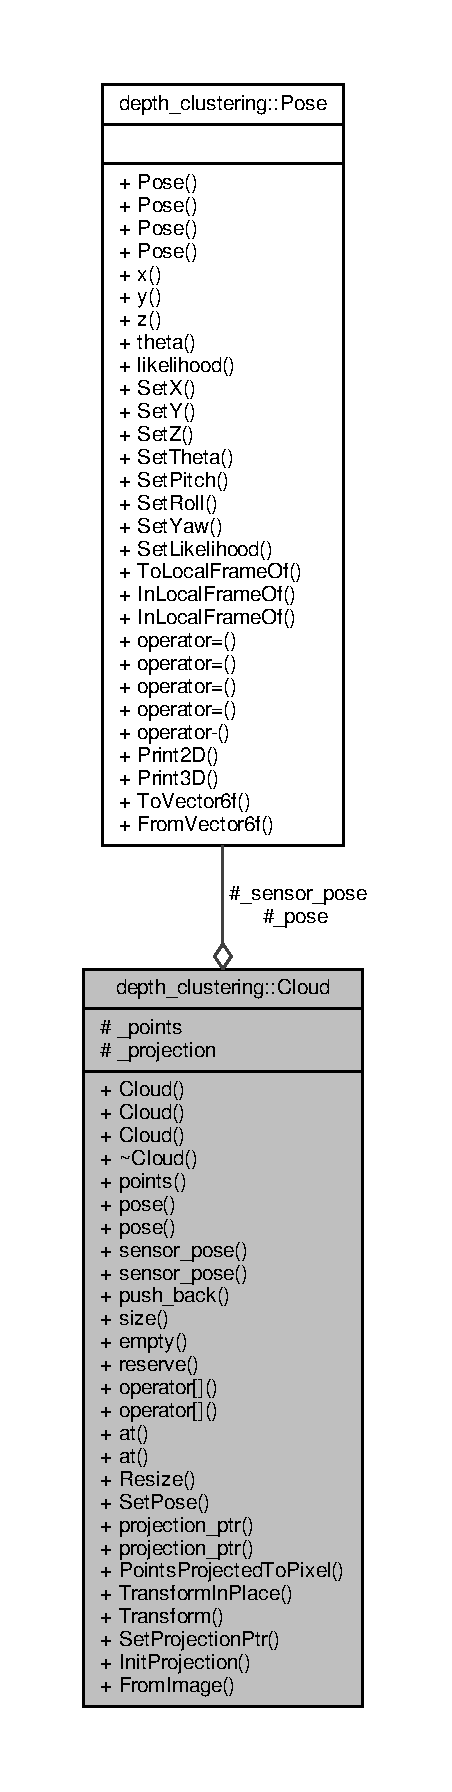
\includegraphics[height=550pt]{classdepth__clustering_1_1Cloud__coll__graph}
\end{center}
\end{figure}


The documentation for this class was generated from the following files\-:\begin{DoxyCompactItemize}
\item 
/home/hadoop/chy/depth\-\_\-clustering-\/master234/src/utils/cloud.\-h\item 
/home/hadoop/chy/depth\-\_\-clustering-\/master234/src/utils/cloud.\-cpp\end{DoxyCompactItemize}

\hypertarget{classdepth__clustering_1_1CloudOdomRosSubscriber}{\section{depth\-\_\-clustering\-:\-:Cloud\-Odom\-Ros\-Subscriber Class Reference}
\label{classdepth__clustering_1_1CloudOdomRosSubscriber}\index{depth\-\_\-clustering\-::\-Cloud\-Odom\-Ros\-Subscriber@{depth\-\_\-clustering\-::\-Cloud\-Odom\-Ros\-Subscriber}}
}


Class for cloud odom ros subscriber.  




{\ttfamily \#include $<$cloud\-\_\-odom\-\_\-ros\-\_\-subscriber.\-h$>$}

\subsection*{Public Member Functions}
\begin{DoxyCompactItemize}
\item 
\hypertarget{classdepth__clustering_1_1CloudOdomRosSubscriber_a01d66910b5dfe1d1145a8d68645bd7b4}{{\bfseries Cloud\-Odom\-Ros\-Subscriber} (ros\-::\-Node\-Handle $\ast$node\-\_\-handle, const \hyperlink{classdepth__clustering_1_1ProjectionParams}{Projection\-Params} \&params, const std\-::string \&topic\-\_\-clouds, const std\-::string \&topic\-\_\-odom=\char`\"{}\char`\"{})}\label{classdepth__clustering_1_1CloudOdomRosSubscriber_a01d66910b5dfe1d1145a8d68645bd7b4}

\item 
void \hyperlink{classdepth__clustering_1_1CloudOdomRosSubscriber_a76a7474f1deed190ac2fb57084c4cdb9}{Callback} (const Point\-Cloud\-T\-::\-Const\-Ptr \&msg\-\_\-cloud, const Odometry\-T\-::\-Const\-Ptr \&msg\-\_\-odom)
\begin{DoxyCompactList}\small\item\em Get synchronized odometry and cloud. \end{DoxyCompactList}\item 
void \hyperlink{classdepth__clustering_1_1CloudOdomRosSubscriber_a8de806bc0b847229dcc92c504908f019}{Callback\-Velodyne} (const sensor\-\_\-msgs\-::\-Point\-Cloud2\-::\-Const\-Ptr \&msg\-\_\-cloud)
\begin{DoxyCompactList}\small\item\em Get point cloud from R\-O\-S. \end{DoxyCompactList}\item 
\hypertarget{classdepth__clustering_1_1CloudOdomRosSubscriber_a16020c63b14308591cae6f4a9ba9b29a}{void \hyperlink{classdepth__clustering_1_1CloudOdomRosSubscriber_a16020c63b14308591cae6f4a9ba9b29a}{Start\-Listening\-To\-Ros} ()}\label{classdepth__clustering_1_1CloudOdomRosSubscriber_a16020c63b14308591cae6f4a9ba9b29a}

\begin{DoxyCompactList}\small\item\em Starts listening to ros. \end{DoxyCompactList}\end{DoxyCompactItemize}
\subsection*{Protected Member Functions}
\begin{DoxyCompactItemize}
\item 
\hypertarget{classdepth__clustering_1_1CloudOdomRosSubscriber_a2a5fac22f067b9cbfd395814c6939d8a}{\hyperlink{classdepth__clustering_1_1Pose}{Pose} {\bfseries Ros\-Odom\-To\-Pose} (const Odometry\-T\-::\-Const\-Ptr \&msg)}\label{classdepth__clustering_1_1CloudOdomRosSubscriber_a2a5fac22f067b9cbfd395814c6939d8a}

\item 
\hypertarget{classdepth__clustering_1_1CloudOdomRosSubscriber_ad80bb8e5ba1f5f21221233145337c5eb}{Cloud\-::\-Ptr {\bfseries Ros\-Cloud\-To\-Cloud} (const Point\-Cloud\-T\-::\-Const\-Ptr \&msg)}\label{classdepth__clustering_1_1CloudOdomRosSubscriber_ad80bb8e5ba1f5f21221233145337c5eb}

\end{DoxyCompactItemize}
\subsection*{Protected Attributes}
\begin{DoxyCompactItemize}
\item 
\hypertarget{classdepth__clustering_1_1CloudOdomRosSubscriber_af44b4e9d0bfe1c030324ea4600a8d49e}{ros\-::\-Node\-Handle $\ast$ {\bfseries \-\_\-node\-\_\-handle}}\label{classdepth__clustering_1_1CloudOdomRosSubscriber_af44b4e9d0bfe1c030324ea4600a8d49e}

\item 
\hypertarget{classdepth__clustering_1_1CloudOdomRosSubscriber_a47a509c60650a113d7aba3a36c7a6a17}{message\-\_\-filters\-::\-Subscriber\\*
$<$ Point\-Cloud\-T $>$ $\ast$ {\bfseries \-\_\-subscriber\-\_\-clouds}}\label{classdepth__clustering_1_1CloudOdomRosSubscriber_a47a509c60650a113d7aba3a36c7a6a17}

\item 
\hypertarget{classdepth__clustering_1_1CloudOdomRosSubscriber_a869ac4843118077f95777dc483d13873}{message\-\_\-filters\-::\-Subscriber\\*
$<$ Odometry\-T $>$ $\ast$ {\bfseries \-\_\-subscriber\-\_\-odom}}\label{classdepth__clustering_1_1CloudOdomRosSubscriber_a869ac4843118077f95777dc483d13873}

\item 
\hypertarget{classdepth__clustering_1_1CloudOdomRosSubscriber_a4829e587d2ae9c5fee5e3cf753cdeee9}{message\-\_\-filters\-::\-Synchronizer\\*
$<$ Approximate\-Time\-Policy $>$ $\ast$ {\bfseries \-\_\-sync}}\label{classdepth__clustering_1_1CloudOdomRosSubscriber_a4829e587d2ae9c5fee5e3cf753cdeee9}

\item 
\hypertarget{classdepth__clustering_1_1CloudOdomRosSubscriber_ac172f353e2f6fec4d8f07b3a431048a1}{std\-::string {\bfseries \-\_\-topic\-\_\-clouds}}\label{classdepth__clustering_1_1CloudOdomRosSubscriber_ac172f353e2f6fec4d8f07b3a431048a1}

\item 
\hypertarget{classdepth__clustering_1_1CloudOdomRosSubscriber_ad1c0dcb17a16f5611d13afb8e76656e5}{std\-::string {\bfseries \-\_\-topic\-\_\-odom}}\label{classdepth__clustering_1_1CloudOdomRosSubscriber_ad1c0dcb17a16f5611d13afb8e76656e5}

\item 
\hypertarget{classdepth__clustering_1_1CloudOdomRosSubscriber_a0661d98cffa781b355209e71075983b1}{\hyperlink{classdepth__clustering_1_1ProjectionParams}{Projection\-Params} {\bfseries \-\_\-params}}\label{classdepth__clustering_1_1CloudOdomRosSubscriber_a0661d98cffa781b355209e71075983b1}

\item 
\hypertarget{classdepth__clustering_1_1CloudOdomRosSubscriber_a4d9749a4c49ef4c91807ab2a573e33fe}{int {\bfseries \-\_\-msg\-\_\-queue\-\_\-size}}\label{classdepth__clustering_1_1CloudOdomRosSubscriber_a4d9749a4c49ef4c91807ab2a573e33fe}

\end{DoxyCompactItemize}
\subsection*{Additional Inherited Members}


\subsection{Detailed Description}
Class for cloud odom ros subscriber. 

Inheritance diagram for depth\-\_\-clustering\-:\-:Cloud\-Odom\-Ros\-Subscriber\-:
\nopagebreak
\begin{figure}[H]
\begin{center}
\leavevmode
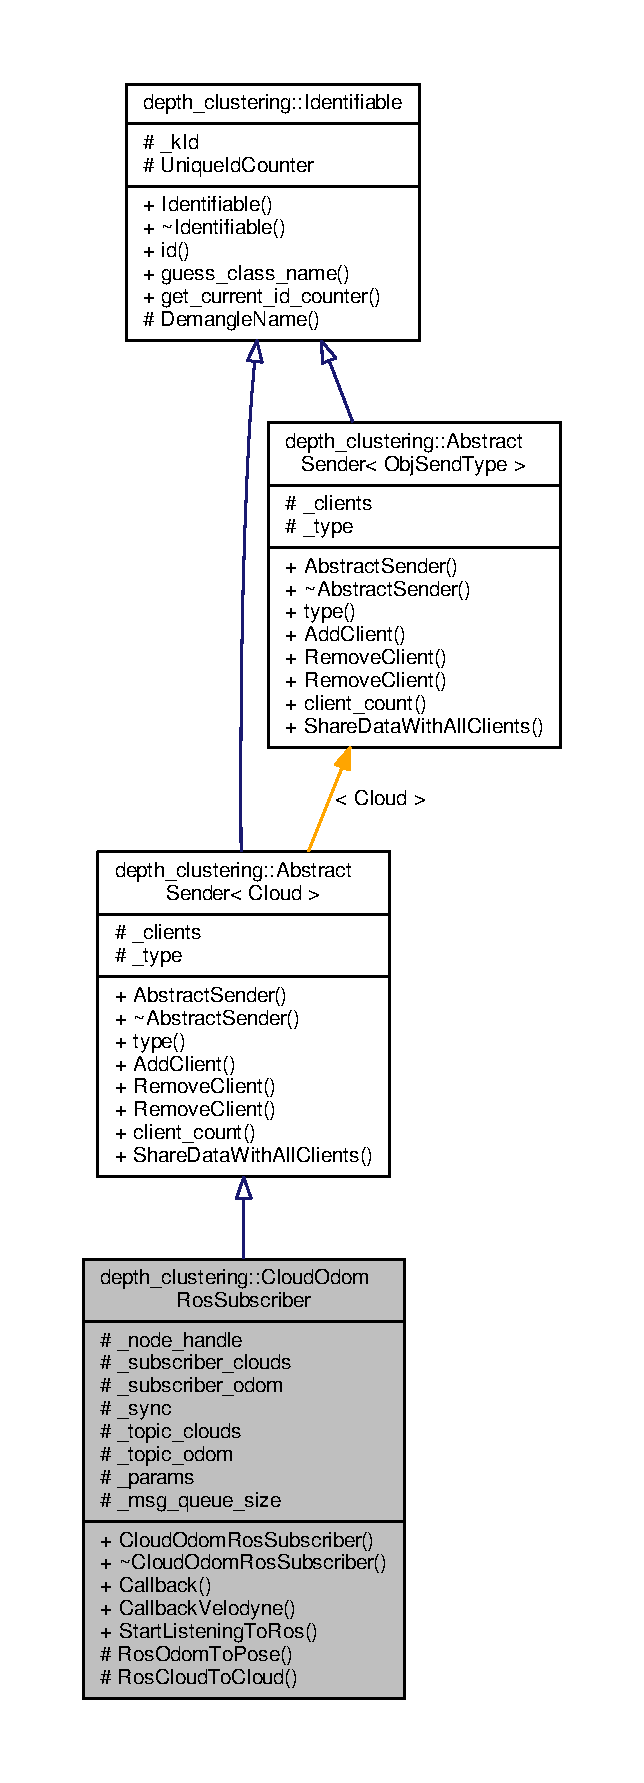
\includegraphics[height=550pt]{classdepth__clustering_1_1CloudOdomRosSubscriber__inherit__graph}
\end{center}
\end{figure}


Collaboration diagram for depth\-\_\-clustering\-:\-:Cloud\-Odom\-Ros\-Subscriber\-:
\nopagebreak
\begin{figure}[H]
\begin{center}
\leavevmode
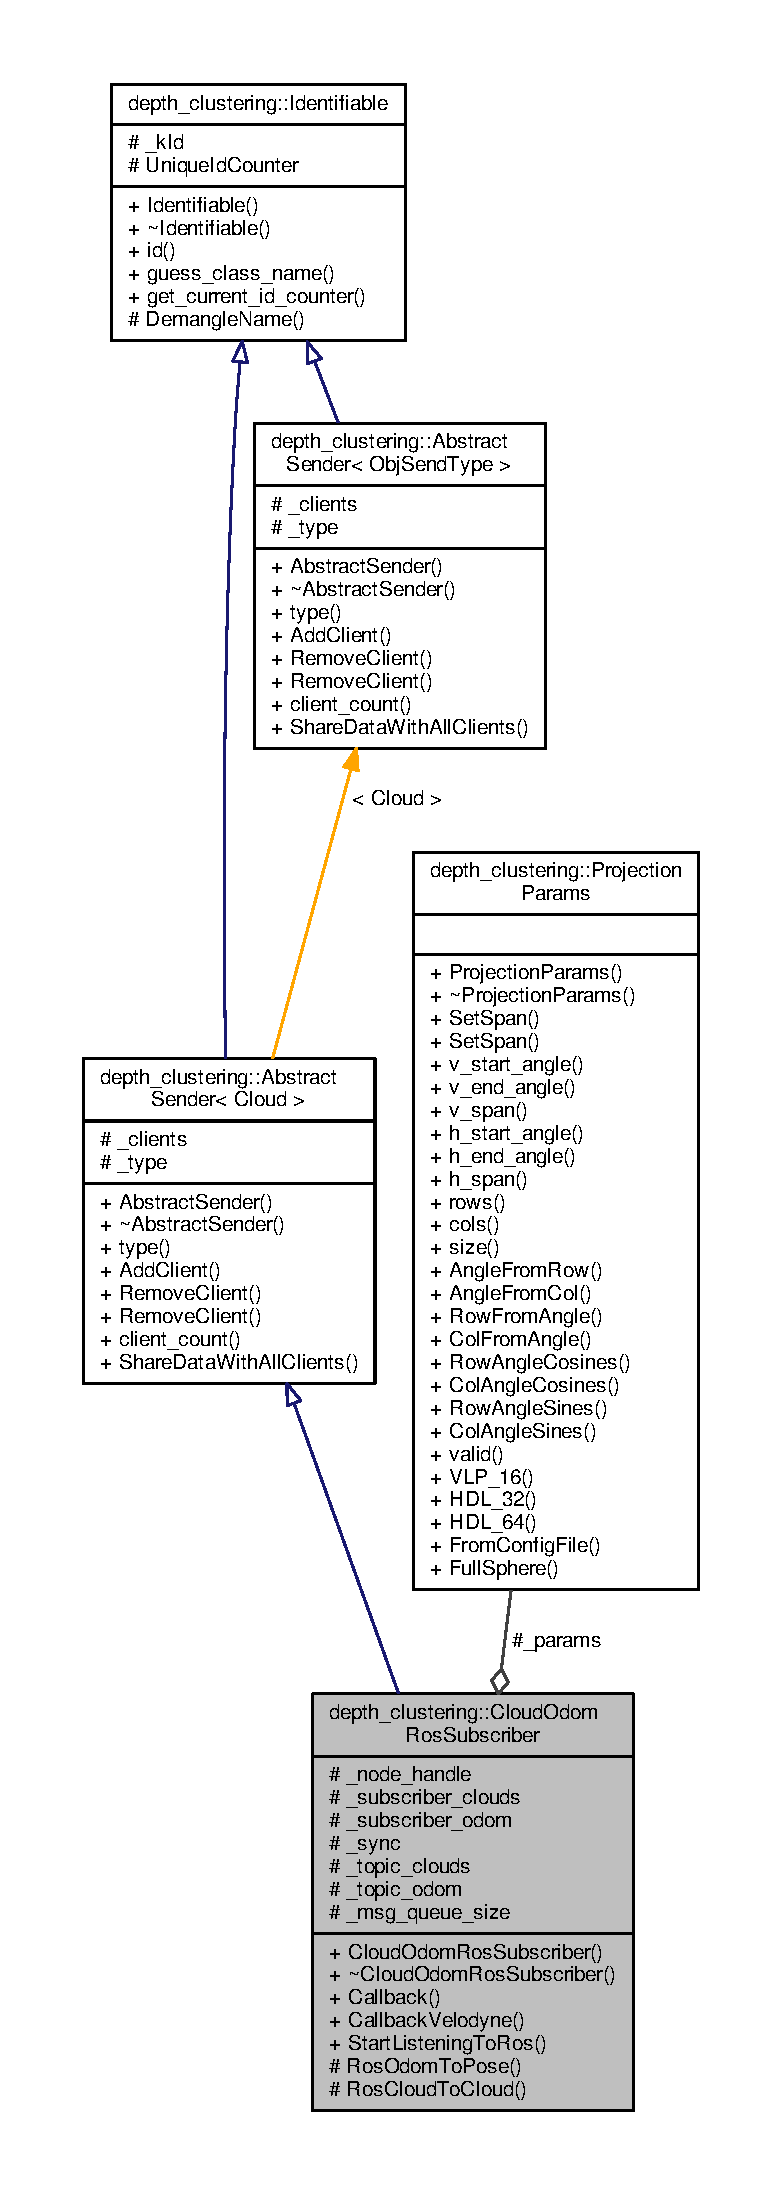
\includegraphics[height=550pt]{classdepth__clustering_1_1CloudOdomRosSubscriber__coll__graph}
\end{center}
\end{figure}


\subsection{Member Function Documentation}
\hypertarget{classdepth__clustering_1_1CloudOdomRosSubscriber_a76a7474f1deed190ac2fb57084c4cdb9}{\index{depth\-\_\-clustering\-::\-Cloud\-Odom\-Ros\-Subscriber@{depth\-\_\-clustering\-::\-Cloud\-Odom\-Ros\-Subscriber}!Callback@{Callback}}
\index{Callback@{Callback}!depth_clustering::CloudOdomRosSubscriber@{depth\-\_\-clustering\-::\-Cloud\-Odom\-Ros\-Subscriber}}
\subsubsection[{Callback}]{\setlength{\rightskip}{0pt plus 5cm}void depth\-\_\-clustering\-::\-Cloud\-Odom\-Ros\-Subscriber\-::\-Callback (
\begin{DoxyParamCaption}
\item[{const Point\-Cloud\-T\-::\-Const\-Ptr \&}]{msg\-\_\-cloud, }
\item[{const Odometry\-T\-::\-Const\-Ptr \&}]{msg\-\_\-odom}
\end{DoxyParamCaption}
)}}\label{classdepth__clustering_1_1CloudOdomRosSubscriber_a76a7474f1deed190ac2fb57084c4cdb9}


Get synchronized odometry and cloud. 


\begin{DoxyParams}[1]{Parameters}
\mbox{\tt in}  & {\em msg\-\_\-cloud} & The message cloud \\
\hline
\mbox{\tt in}  & {\em msg\-\_\-odom} & The message odom \\
\hline
\end{DoxyParams}


Here is the call graph for this function\-:
\nopagebreak
\begin{figure}[H]
\begin{center}
\leavevmode
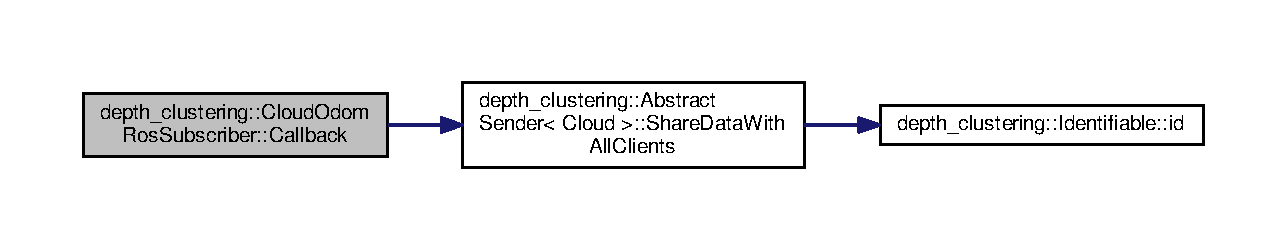
\includegraphics[width=350pt]{classdepth__clustering_1_1CloudOdomRosSubscriber_a76a7474f1deed190ac2fb57084c4cdb9_cgraph}
\end{center}
\end{figure}




Here is the caller graph for this function\-:
\nopagebreak
\begin{figure}[H]
\begin{center}
\leavevmode
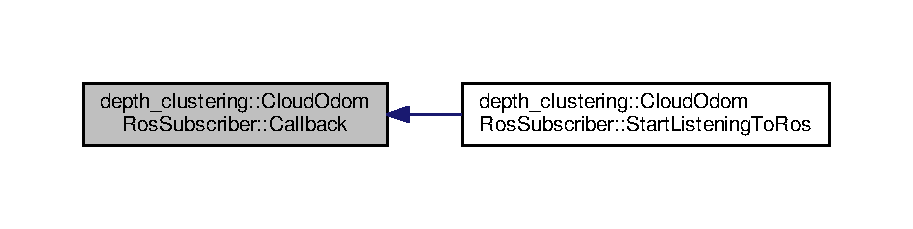
\includegraphics[width=350pt]{classdepth__clustering_1_1CloudOdomRosSubscriber_a76a7474f1deed190ac2fb57084c4cdb9_icgraph}
\end{center}
\end{figure}


\hypertarget{classdepth__clustering_1_1CloudOdomRosSubscriber_a8de806bc0b847229dcc92c504908f019}{\index{depth\-\_\-clustering\-::\-Cloud\-Odom\-Ros\-Subscriber@{depth\-\_\-clustering\-::\-Cloud\-Odom\-Ros\-Subscriber}!Callback\-Velodyne@{Callback\-Velodyne}}
\index{Callback\-Velodyne@{Callback\-Velodyne}!depth_clustering::CloudOdomRosSubscriber@{depth\-\_\-clustering\-::\-Cloud\-Odom\-Ros\-Subscriber}}
\subsubsection[{Callback\-Velodyne}]{\setlength{\rightskip}{0pt plus 5cm}void depth\-\_\-clustering\-::\-Cloud\-Odom\-Ros\-Subscriber\-::\-Callback\-Velodyne (
\begin{DoxyParamCaption}
\item[{const sensor\-\_\-msgs\-::\-Point\-Cloud2\-::\-Const\-Ptr \&}]{msg\-\_\-cloud}
\end{DoxyParamCaption}
)}}\label{classdepth__clustering_1_1CloudOdomRosSubscriber_a8de806bc0b847229dcc92c504908f019}


Get point cloud from R\-O\-S. 


\begin{DoxyParams}[1]{Parameters}
\mbox{\tt in}  & {\em msg\-\_\-cloud} & The message cloud \\
\hline
\end{DoxyParams}


Here is the call graph for this function\-:
\nopagebreak
\begin{figure}[H]
\begin{center}
\leavevmode
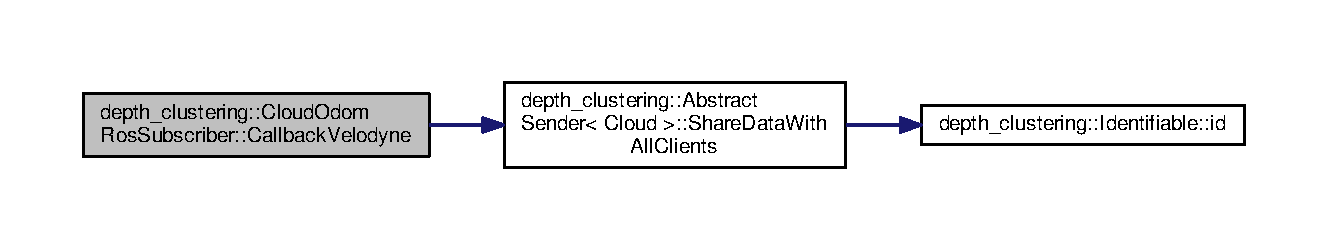
\includegraphics[width=350pt]{classdepth__clustering_1_1CloudOdomRosSubscriber_a8de806bc0b847229dcc92c504908f019_cgraph}
\end{center}
\end{figure}




Here is the caller graph for this function\-:
\nopagebreak
\begin{figure}[H]
\begin{center}
\leavevmode
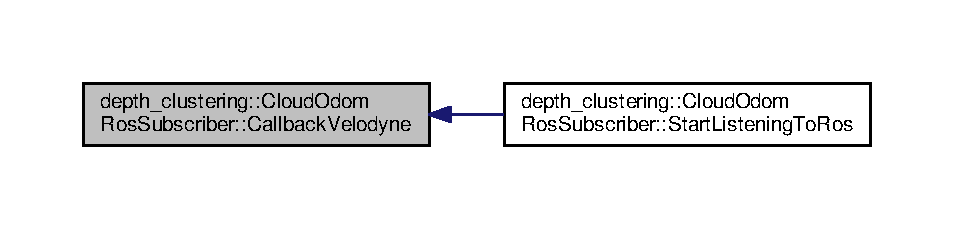
\includegraphics[width=350pt]{classdepth__clustering_1_1CloudOdomRosSubscriber_a8de806bc0b847229dcc92c504908f019_icgraph}
\end{center}
\end{figure}




The documentation for this class was generated from the following files\-:\begin{DoxyCompactItemize}
\item 
/home/hadoop/chy/depth\-\_\-clustering-\/master234/src/ros\-\_\-bridge/cloud\-\_\-odom\-\_\-ros\-\_\-subscriber.\-h\item 
/home/hadoop/chy/depth\-\_\-clustering-\/master234/src/ros\-\_\-bridge/cloud\-\_\-odom\-\_\-ros\-\_\-subscriber.\-cpp\end{DoxyCompactItemize}

\hypertarget{classdepth__clustering_1_1CloudProjection}{\section{depth\-\_\-clustering\-:\-:Cloud\-Projection Class Reference}
\label{classdepth__clustering_1_1CloudProjection}\index{depth\-\_\-clustering\-::\-Cloud\-Projection@{depth\-\_\-clustering\-::\-Cloud\-Projection}}
}


Abstract class for cloud projection.  




{\ttfamily \#include $<$cloud\-\_\-projection.\-h$>$}

\subsection*{Classes}
\begin{DoxyCompactItemize}
\item 
class \hyperlink{classdepth__clustering_1_1CloudProjection_1_1PointContainer}{Point\-Container}
\begin{DoxyCompactList}\small\item\em Class for point container. \end{DoxyCompactList}\end{DoxyCompactItemize}
\subsection*{Public Types}
\begin{DoxyCompactItemize}
\item 
enum {\bfseries Type} \{ {\bfseries S\-P\-H\-E\-R\-I\-C\-A\-L}, 
{\bfseries C\-Y\-L\-L\-I\-N\-D\-R\-I\-C\-A\-L}
 \}
\item 
\hypertarget{classdepth__clustering_1_1CloudProjection_a7ac49f27b97e149be239a777587b4162}{using {\bfseries Ptr} = shared\-\_\-ptr$<$ \hyperlink{classdepth__clustering_1_1CloudProjection}{Cloud\-Projection} $>$}\label{classdepth__clustering_1_1CloudProjection_a7ac49f27b97e149be239a777587b4162}

\item 
\hypertarget{classdepth__clustering_1_1CloudProjection_aa7a2a7f37a6ebd5533e336e1f484567a}{using {\bfseries Const\-Ptr} = shared\-\_\-ptr$<$ const \hyperlink{classdepth__clustering_1_1CloudProjection}{Cloud\-Projection} $>$}\label{classdepth__clustering_1_1CloudProjection_aa7a2a7f37a6ebd5533e336e1f484567a}

\end{DoxyCompactItemize}
\subsection*{Public Member Functions}
\begin{DoxyCompactItemize}
\item 
\hypertarget{classdepth__clustering_1_1CloudProjection_a7abfd6e56bacd684379916af2ab60cef}{{\bfseries Cloud\-Projection} (const \hyperlink{classdepth__clustering_1_1ProjectionParams}{Projection\-Params} \&params)}\label{classdepth__clustering_1_1CloudProjection_a7abfd6e56bacd684379916af2ab60cef}

\item 
virtual void \hyperlink{classdepth__clustering_1_1CloudProjection_ad262ef9f4e0c9c7fab9cc37874ca72eb}{Init\-From\-Points} (const std\-::vector$<$ \hyperlink{classdepth__clustering_1_1RichPoint}{Rich\-Point} $>$ \&points)=0
\begin{DoxyCompactList}\small\item\em Initialize from 3d points. \end{DoxyCompactList}\item 
virtual Cloud\-Projection\-::\-Ptr \hyperlink{classdepth__clustering_1_1CloudProjection_ae06ff9699c1a37c535b39fa6f722fa2e}{Clone} () const =0
\begin{DoxyCompactList}\small\item\em Polymorphic clone of a projection. \end{DoxyCompactList}\item 
\hypertarget{classdepth__clustering_1_1CloudProjection_a5519c93050ed140d8baace3a625fd9ed}{const cv\-::\-Mat \& {\bfseries depth\-\_\-image} () const }\label{classdepth__clustering_1_1CloudProjection_a5519c93050ed140d8baace3a625fd9ed}

\item 
\hypertarget{classdepth__clustering_1_1CloudProjection_aa04e09c527c7e1bc1b5ab161c5931b30}{cv\-::\-Mat \& {\bfseries depth\-\_\-image} ()}\label{classdepth__clustering_1_1CloudProjection_aa04e09c527c7e1bc1b5ab161c5931b30}

\item 
\hypertarget{classdepth__clustering_1_1CloudProjection_a3e28dfda41fa497bfd54fe3c7f2a9b37}{void {\bfseries Clone\-Depth\-Image} (const cv\-::\-Mat \&image)}\label{classdepth__clustering_1_1CloudProjection_a3e28dfda41fa497bfd54fe3c7f2a9b37}

\item 
\hypertarget{classdepth__clustering_1_1CloudProjection_a41fe972471286f13a15167860a0d6fce}{size\-\_\-t {\bfseries rows} () const }\label{classdepth__clustering_1_1CloudProjection_a41fe972471286f13a15167860a0d6fce}

\item 
\hypertarget{classdepth__clustering_1_1CloudProjection_a777b6b7040065187e2ab19656078f1a2}{size\-\_\-t {\bfseries cols} () const }\label{classdepth__clustering_1_1CloudProjection_a777b6b7040065187e2ab19656078f1a2}

\item 
\hypertarget{classdepth__clustering_1_1CloudProjection_a64d4cdc9a3faedc42ae3b40b1fcbd5d2}{size\-\_\-t {\bfseries size} () const }\label{classdepth__clustering_1_1CloudProjection_a64d4cdc9a3faedc42ae3b40b1fcbd5d2}

\item 
\hypertarget{classdepth__clustering_1_1CloudProjection_a8ce8f68e2f29d6cd4dbfda1a7bee6c13}{const \hyperlink{classdepth__clustering_1_1ProjectionParams}{Projection\-Params} \& {\bfseries params} () const }\label{classdepth__clustering_1_1CloudProjection_a8ce8f68e2f29d6cd4dbfda1a7bee6c13}

\item 
\hypertarget{classdepth__clustering_1_1CloudProjection_a5bb974dd99ff9e840d1c48b3d8a56fc8}{const \hyperlink{classdepth__clustering_1_1CloudProjection_1_1PointContainer}{Point\-Container} \& {\bfseries at} (const size\-\_\-t row, const size\-\_\-t col) const }\label{classdepth__clustering_1_1CloudProjection_a5bb974dd99ff9e840d1c48b3d8a56fc8}

\item 
\hypertarget{classdepth__clustering_1_1CloudProjection_a72001e572391d9fba69f2572ac6369f5}{\hyperlink{classdepth__clustering_1_1CloudProjection_1_1PointContainer}{Point\-Container} \& {\bfseries at} (const size\-\_\-t row, const size\-\_\-t col)}\label{classdepth__clustering_1_1CloudProjection_a72001e572391d9fba69f2572ac6369f5}

\item 
\hypertarget{classdepth__clustering_1_1CloudProjection_ae61165968d75b56863d09bd8cd48e91e}{const Point\-Matrix \& {\bfseries matrix} () const }\label{classdepth__clustering_1_1CloudProjection_ae61165968d75b56863d09bd8cd48e91e}

\item 
void \hyperlink{classdepth__clustering_1_1CloudProjection_ad92d5819092ef3e4aabd4da3a5775f38}{Check\-Image\-And\-Storage} (const cv\-::\-Mat \&image)
\begin{DoxyCompactList}\small\item\em Check if where we store data is valid. \end{DoxyCompactList}\item 
void \hyperlink{classdepth__clustering_1_1CloudProjection_a595aa7f47ea9a934aaadff11f3709070}{Check\-Cloud\-And\-Storage} (const std\-::vector$<$ \hyperlink{classdepth__clustering_1_1RichPoint}{Rich\-Point} $>$ \&points)
\begin{DoxyCompactList}\small\item\em Check if where we store data is valid. \end{DoxyCompactList}\item 
virtual \hyperlink{classdepth__clustering_1_1RichPoint}{Rich\-Point} \hyperlink{classdepth__clustering_1_1CloudProjection_a684ca31033ee3b6b9d0ba2ea86d6e5b9}{Unproject\-Point} (const cv\-::\-Mat \&image, const int row, const int col) const 
\begin{DoxyCompactList}\small\item\em Unproject a point from depth image coordinate. \end{DoxyCompactList}\end{DoxyCompactItemize}
\subsection*{Protected Attributes}
\begin{DoxyCompactItemize}
\item 
\hypertarget{classdepth__clustering_1_1CloudProjection_a3f70579b10bd93a7d5ac4b1f0d387701}{Point\-Matrix {\bfseries \-\_\-data}}\label{classdepth__clustering_1_1CloudProjection_a3f70579b10bd93a7d5ac4b1f0d387701}

\item 
\hypertarget{classdepth__clustering_1_1CloudProjection_a8978a85d52212a2a88cbb3c6791eddd6}{\hyperlink{classdepth__clustering_1_1ProjectionParams}{Projection\-Params} {\bfseries \-\_\-params}}\label{classdepth__clustering_1_1CloudProjection_a8978a85d52212a2a88cbb3c6791eddd6}

\item 
\hypertarget{classdepth__clustering_1_1CloudProjection_a2d239a9a0fcaada00de36aad436e2af2}{cv\-::\-Mat {\bfseries \-\_\-depth\-\_\-image}}\label{classdepth__clustering_1_1CloudProjection_a2d239a9a0fcaada00de36aad436e2af2}

\end{DoxyCompactItemize}


\subsection{Detailed Description}
Abstract class for cloud projection. 

Inheritance diagram for depth\-\_\-clustering\-:\-:Cloud\-Projection\-:
\nopagebreak
\begin{figure}[H]
\begin{center}
\leavevmode
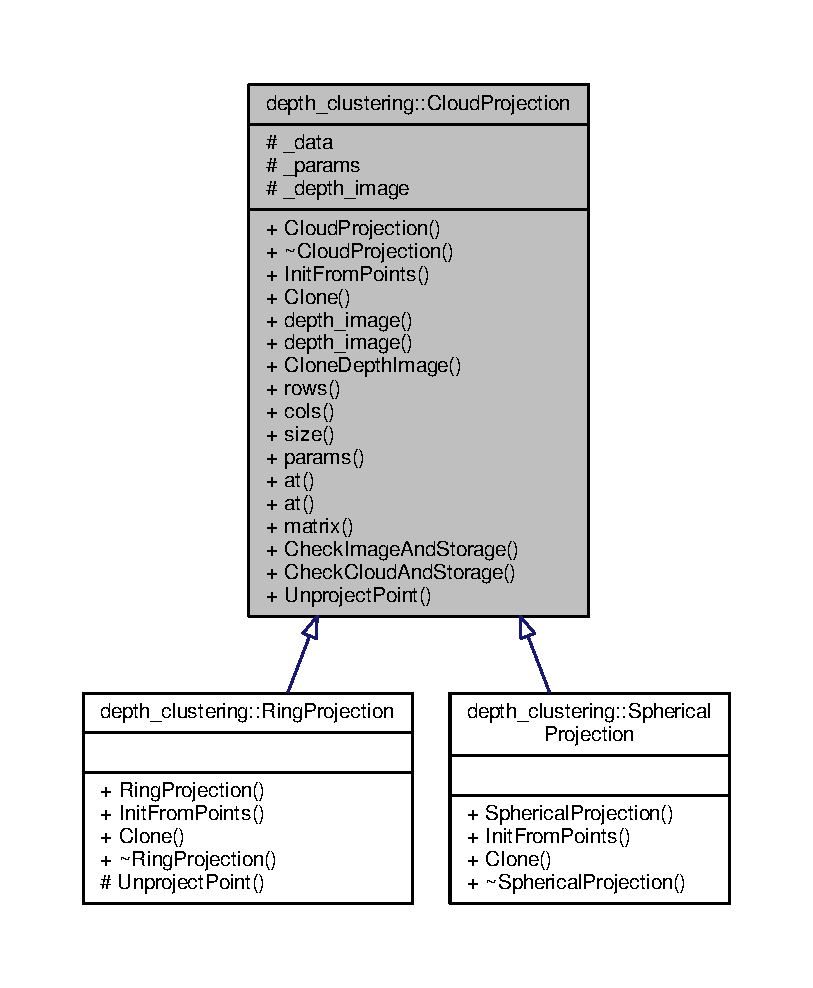
\includegraphics[width=350pt]{classdepth__clustering_1_1CloudProjection__inherit__graph}
\end{center}
\end{figure}


Collaboration diagram for depth\-\_\-clustering\-:\-:Cloud\-Projection\-:
\nopagebreak
\begin{figure}[H]
\begin{center}
\leavevmode
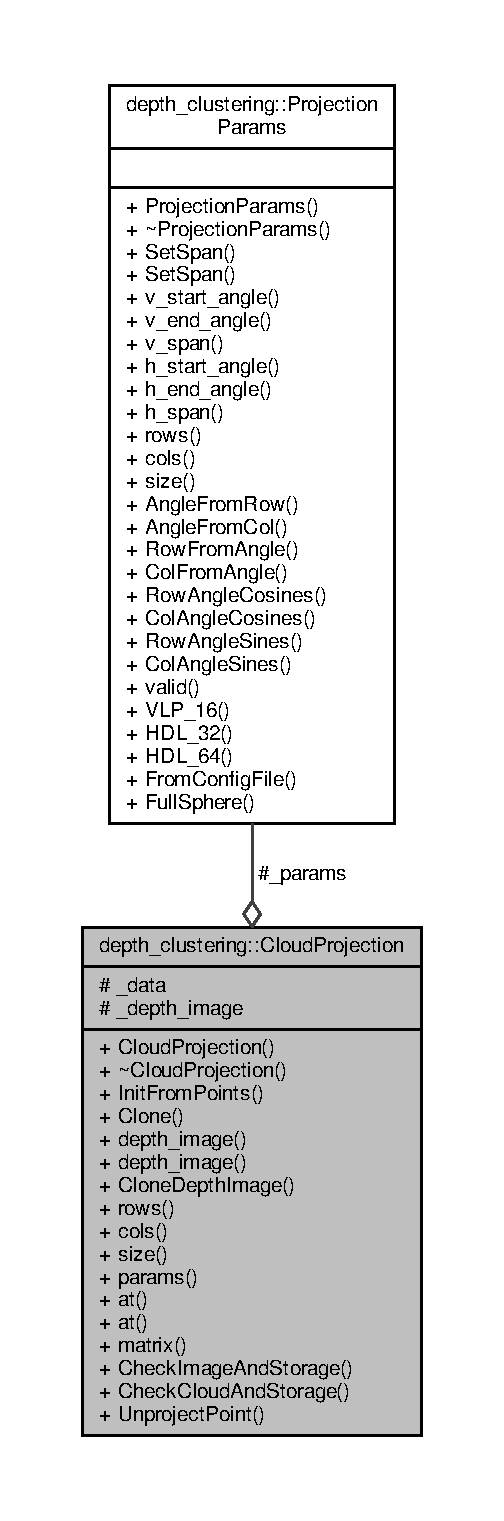
\includegraphics[height=550pt]{classdepth__clustering_1_1CloudProjection__coll__graph}
\end{center}
\end{figure}


\subsection{Member Function Documentation}
\hypertarget{classdepth__clustering_1_1CloudProjection_a595aa7f47ea9a934aaadff11f3709070}{\index{depth\-\_\-clustering\-::\-Cloud\-Projection@{depth\-\_\-clustering\-::\-Cloud\-Projection}!Check\-Cloud\-And\-Storage@{Check\-Cloud\-And\-Storage}}
\index{Check\-Cloud\-And\-Storage@{Check\-Cloud\-And\-Storage}!depth_clustering::CloudProjection@{depth\-\_\-clustering\-::\-Cloud\-Projection}}
\subsubsection[{Check\-Cloud\-And\-Storage}]{\setlength{\rightskip}{0pt plus 5cm}void depth\-\_\-clustering\-::\-Cloud\-Projection\-::\-Check\-Cloud\-And\-Storage (
\begin{DoxyParamCaption}
\item[{const std\-::vector$<$ {\bf Rich\-Point} $>$ \&}]{points}
\end{DoxyParamCaption}
)}}\label{classdepth__clustering_1_1CloudProjection_a595aa7f47ea9a934aaadff11f3709070}


Check if where we store data is valid. 


\begin{DoxyParams}[1]{Parameters}
\mbox{\tt in}  & {\em points} & The points to check \\
\hline
\end{DoxyParams}


Here is the caller graph for this function\-:
\nopagebreak
\begin{figure}[H]
\begin{center}
\leavevmode
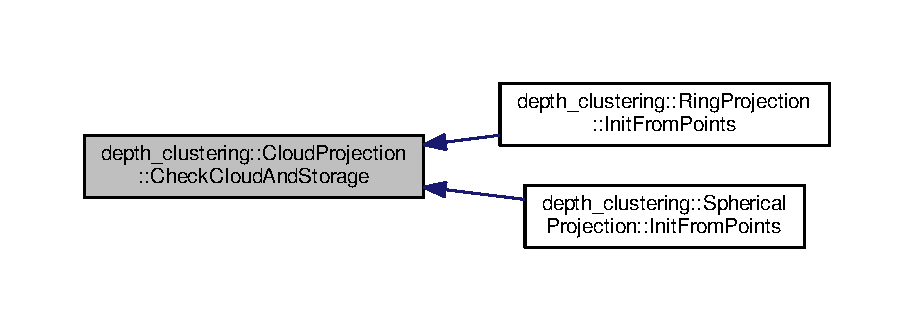
\includegraphics[width=350pt]{classdepth__clustering_1_1CloudProjection_a595aa7f47ea9a934aaadff11f3709070_icgraph}
\end{center}
\end{figure}


\hypertarget{classdepth__clustering_1_1CloudProjection_ad92d5819092ef3e4aabd4da3a5775f38}{\index{depth\-\_\-clustering\-::\-Cloud\-Projection@{depth\-\_\-clustering\-::\-Cloud\-Projection}!Check\-Image\-And\-Storage@{Check\-Image\-And\-Storage}}
\index{Check\-Image\-And\-Storage@{Check\-Image\-And\-Storage}!depth_clustering::CloudProjection@{depth\-\_\-clustering\-::\-Cloud\-Projection}}
\subsubsection[{Check\-Image\-And\-Storage}]{\setlength{\rightskip}{0pt plus 5cm}void depth\-\_\-clustering\-::\-Cloud\-Projection\-::\-Check\-Image\-And\-Storage (
\begin{DoxyParamCaption}
\item[{const cv\-::\-Mat \&}]{image}
\end{DoxyParamCaption}
)}}\label{classdepth__clustering_1_1CloudProjection_ad92d5819092ef3e4aabd4da3a5775f38}


Check if where we store data is valid. 


\begin{DoxyParams}[1]{Parameters}
\mbox{\tt in}  & {\em image} & The image to check \\
\hline
\end{DoxyParams}
\hypertarget{classdepth__clustering_1_1CloudProjection_ae06ff9699c1a37c535b39fa6f722fa2e}{\index{depth\-\_\-clustering\-::\-Cloud\-Projection@{depth\-\_\-clustering\-::\-Cloud\-Projection}!Clone@{Clone}}
\index{Clone@{Clone}!depth_clustering::CloudProjection@{depth\-\_\-clustering\-::\-Cloud\-Projection}}
\subsubsection[{Clone}]{\setlength{\rightskip}{0pt plus 5cm}virtual Cloud\-Projection\-::\-Ptr depth\-\_\-clustering\-::\-Cloud\-Projection\-::\-Clone (
\begin{DoxyParamCaption}
{}
\end{DoxyParamCaption}
) const\hspace{0.3cm}{\ttfamily [pure virtual]}}}\label{classdepth__clustering_1_1CloudProjection_ae06ff9699c1a37c535b39fa6f722fa2e}


Polymorphic clone of a projection. 

\begin{DoxyReturn}{Returns}
Shared pointer of a copy of this object. 
\end{DoxyReturn}


Implemented in \hyperlink{classdepth__clustering_1_1RingProjection_a433c0ee114b89b6c78ad4c471d120153}{depth\-\_\-clustering\-::\-Ring\-Projection}, and \hyperlink{classdepth__clustering_1_1SphericalProjection_a1b7870502497310666b2909701906470}{depth\-\_\-clustering\-::\-Spherical\-Projection}.

\hypertarget{classdepth__clustering_1_1CloudProjection_ad262ef9f4e0c9c7fab9cc37874ca72eb}{\index{depth\-\_\-clustering\-::\-Cloud\-Projection@{depth\-\_\-clustering\-::\-Cloud\-Projection}!Init\-From\-Points@{Init\-From\-Points}}
\index{Init\-From\-Points@{Init\-From\-Points}!depth_clustering::CloudProjection@{depth\-\_\-clustering\-::\-Cloud\-Projection}}
\subsubsection[{Init\-From\-Points}]{\setlength{\rightskip}{0pt plus 5cm}virtual void depth\-\_\-clustering\-::\-Cloud\-Projection\-::\-Init\-From\-Points (
\begin{DoxyParamCaption}
\item[{const std\-::vector$<$ {\bf Rich\-Point} $>$ \&}]{points}
\end{DoxyParamCaption}
)\hspace{0.3cm}{\ttfamily [pure virtual]}}}\label{classdepth__clustering_1_1CloudProjection_ad262ef9f4e0c9c7fab9cc37874ca72eb}


Initialize from 3d points. 


\begin{DoxyParams}[1]{Parameters}
\mbox{\tt in}  & {\em points} & The points \\
\hline
\end{DoxyParams}


Implemented in \hyperlink{classdepth__clustering_1_1RingProjection_af2984815f24bc0a8c131c233d319268c}{depth\-\_\-clustering\-::\-Ring\-Projection}, and \hyperlink{classdepth__clustering_1_1SphericalProjection_a36daf4acaed7ded443dd1928f27e7bb8}{depth\-\_\-clustering\-::\-Spherical\-Projection}.

\hypertarget{classdepth__clustering_1_1CloudProjection_a684ca31033ee3b6b9d0ba2ea86d6e5b9}{\index{depth\-\_\-clustering\-::\-Cloud\-Projection@{depth\-\_\-clustering\-::\-Cloud\-Projection}!Unproject\-Point@{Unproject\-Point}}
\index{Unproject\-Point@{Unproject\-Point}!depth_clustering::CloudProjection@{depth\-\_\-clustering\-::\-Cloud\-Projection}}
\subsubsection[{Unproject\-Point}]{\setlength{\rightskip}{0pt plus 5cm}{\bf Rich\-Point} depth\-\_\-clustering\-::\-Cloud\-Projection\-::\-Unproject\-Point (
\begin{DoxyParamCaption}
\item[{const cv\-::\-Mat \&}]{image, }
\item[{const int}]{row, }
\item[{const int}]{col}
\end{DoxyParamCaption}
) const\hspace{0.3cm}{\ttfamily [virtual]}}}\label{classdepth__clustering_1_1CloudProjection_a684ca31033ee3b6b9d0ba2ea86d6e5b9}


Unproject a point from depth image coordinate. 


\begin{DoxyParams}[1]{Parameters}
\mbox{\tt in}  & {\em image} & A depth image \\
\hline
\mbox{\tt in}  & {\em row} & A row in the image \\
\hline
\mbox{\tt in}  & {\em col} & A col in the image\\
\hline
\end{DoxyParams}
\begin{DoxyReturn}{Returns}
\{ description\-\_\-of\-\_\-the\-\_\-return\-\_\-value \} 
\end{DoxyReturn}


Reimplemented in \hyperlink{classdepth__clustering_1_1RingProjection_a16cbf43e541e65560cb282c560b4efa7}{depth\-\_\-clustering\-::\-Ring\-Projection}.



Here is the call graph for this function\-:
\nopagebreak
\begin{figure}[H]
\begin{center}
\leavevmode
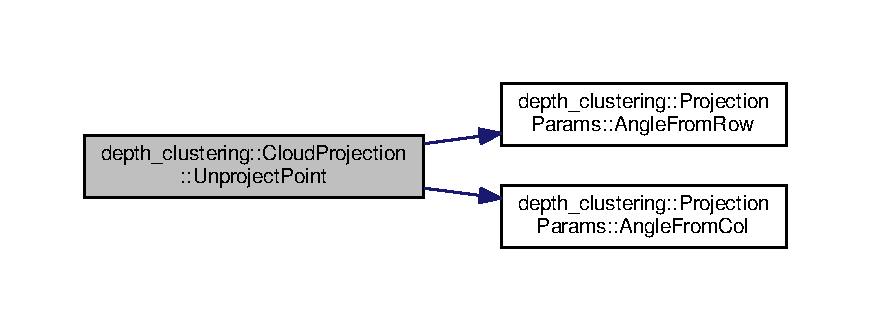
\includegraphics[width=350pt]{classdepth__clustering_1_1CloudProjection_a684ca31033ee3b6b9d0ba2ea86d6e5b9_cgraph}
\end{center}
\end{figure}




Here is the caller graph for this function\-:
\nopagebreak
\begin{figure}[H]
\begin{center}
\leavevmode
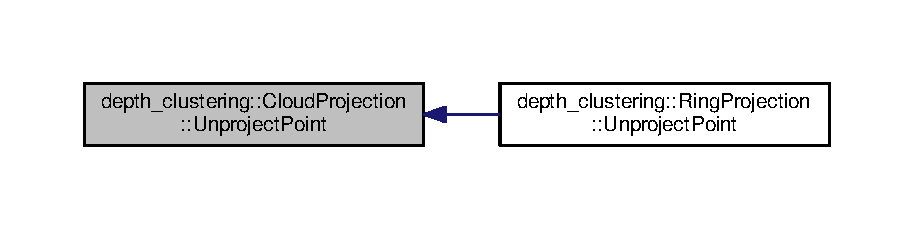
\includegraphics[width=350pt]{classdepth__clustering_1_1CloudProjection_a684ca31033ee3b6b9d0ba2ea86d6e5b9_icgraph}
\end{center}
\end{figure}




The documentation for this class was generated from the following files\-:\begin{DoxyCompactItemize}
\item 
/home/hadoop/chy/depth\-\_\-clustering-\/master234/src/projections/cloud\-\_\-projection.\-h\item 
/home/hadoop/chy/depth\-\_\-clustering-\/master234/src/projections/cloud\-\_\-projection.\-cpp\end{DoxyCompactItemize}

\hypertarget{classdepth__clustering_1_1DepthGroundRemover}{\section{depth\-\_\-clustering\-:\-:Depth\-Ground\-Remover Class Reference}
\label{classdepth__clustering_1_1DepthGroundRemover}\index{depth\-\_\-clustering\-::\-Depth\-Ground\-Remover@{depth\-\_\-clustering\-::\-Depth\-Ground\-Remover}}
}


A class to remove ground based upon depth image.  




{\ttfamily \#include $<$depth\-\_\-ground\-\_\-remover.\-h$>$}

\subsection*{Public Member Functions}
\begin{DoxyCompactItemize}
\item 
\hypertarget{classdepth__clustering_1_1DepthGroundRemover_aae9816017a747246c495de41bcece02c}{{\bfseries Depth\-Ground\-Remover} (const \hyperlink{classdepth__clustering_1_1ProjectionParams}{Projection\-Params} \&params, const Radians \&ground\-\_\-remove\-\_\-angle, int window\-\_\-size=5)}\label{classdepth__clustering_1_1DepthGroundRemover_aae9816017a747246c495de41bcece02c}

\item 
void \hyperlink{classdepth__clustering_1_1DepthGroundRemover_ab2c3bcc8df6cc70ad5057f5ec3bd074f}{On\-New\-Object\-Received} (const \hyperlink{classdepth__clustering_1_1Cloud}{Cloud} \&cloud, const int sender\-\_\-id) override
\begin{DoxyCompactList}\small\item\em when someone sends us an object we process it \end{DoxyCompactList}\end{DoxyCompactItemize}
\subsection*{Protected Member Functions}
\begin{DoxyCompactItemize}
\item 
cv\-::\-Mat \hyperlink{classdepth__clustering_1_1DepthGroundRemover_a0f3733c1cbc915600d255246b1dccce0}{Zero\-Out\-Ground} (const cv\-::\-Mat \&image, const cv\-::\-Mat \&angle\-\_\-image, const Radians \&threshold) const 
\begin{DoxyCompactList}\small\item\em Zero out all pixels that belong to ground 去除掉所有属于地面的点。 \end{DoxyCompactList}\item 
\hypertarget{classdepth__clustering_1_1DepthGroundRemover_a3364e716dc72e6dc2a5d37d6c670a235}{cv\-::\-Mat {\bfseries Zero\-Out\-Ground\-B\-F\-S} (const cv\-::\-Mat \&image, const cv\-::\-Mat \&angle\-\_\-image, const Radians \&threshold, int kernel\-\_\-size) const }\label{classdepth__clustering_1_1DepthGroundRemover_a3364e716dc72e6dc2a5d37d6c670a235}

\item 
cv\-::\-Mat \hyperlink{classdepth__clustering_1_1DepthGroundRemover_af533c51a44aad9a56c12445b61b801b9}{Create\-Angle\-Image} (const cv\-::\-Mat \&depth\-\_\-image)
\begin{DoxyCompactList}\small\item\em create a help image with angle in radians written for each pixel 创建一个帮助图像,角度以弧度为单位编写像素 \end{DoxyCompactList}\item 
cv\-::\-Mat \hyperlink{classdepth__clustering_1_1DepthGroundRemover_a8b660a1be94b529cf2554b8f72aee30d}{Get\-Savitsky\-Golay\-Kernel} (int window\-\_\-size) const 
\begin{DoxyCompactList}\small\item\em Get kernel for Savitsky-\/\-Golay filter为了 滤波器 \end{DoxyCompactList}\item 
\hypertarget{classdepth__clustering_1_1DepthGroundRemover_af3c60a97dd0cca8847e40c86ee11c037}{cv\-::\-Mat {\bfseries Get\-Uniform\-Kernel} (int window\-\_\-size, int \hyperlink{classdepth__clustering_1_1AbstractSender_ad9da304185f766eb4b0035d6610caa49}{type}=C\-V\-\_\-32\-F) const }\label{classdepth__clustering_1_1DepthGroundRemover_af3c60a97dd0cca8847e40c86ee11c037}

\item 
cv\-::\-Mat \hyperlink{classdepth__clustering_1_1DepthGroundRemover_a63b32fa801a13021bf22699525579f8b}{Apply\-Savitsky\-Golay\-Smoothing} (const cv\-::\-Mat \&column, int window\-\_\-size)
\begin{DoxyCompactList}\small\item\em Apply Savitsky-\/\-Golay smoothing to a column. \end{DoxyCompactList}\item 
Radians \hyperlink{classdepth__clustering_1_1DepthGroundRemover_a29ba07a101794aab322ae3c0671806e0}{Get\-Line\-Angle} (const cv\-::\-Mat \&depth\-\_\-image, int col, int row\-\_\-curr, int row\-\_\-neigh)
\begin{DoxyCompactList}\small\item\em Get line angle. \end{DoxyCompactList}\item 
cv\-::\-Mat \hyperlink{classdepth__clustering_1_1DepthGroundRemover_a51dd313ed1bdda2188fb3a3fa1c5738e}{Repair\-Depth} (const cv\-::\-Mat \&no\-\_\-ground\-\_\-image, int step, float depth\-\_\-threshold)
\begin{DoxyCompactList}\small\item\em Repair zeros in the depth image. \end{DoxyCompactList}\item 
\hypertarget{classdepth__clustering_1_1DepthGroundRemover_ab44815e8ea8b10abce24faebf8322624}{cv\-::\-Mat {\bfseries Repair\-Depth} (const cv\-::\-Mat \&depth\-\_\-image)}\label{classdepth__clustering_1_1DepthGroundRemover_ab44815e8ea8b10abce24faebf8322624}

\item 
\hypertarget{classdepth__clustering_1_1DepthGroundRemover_a37cd0a7054c51343f6a25f269890fae2}{void {\bfseries Write\-Data} (cv\-::\-Mat \&m, const char $\ast$filename)}\label{classdepth__clustering_1_1DepthGroundRemover_a37cd0a7054c51343f6a25f269890fae2}

\end{DoxyCompactItemize}
\subsection*{Protected Attributes}
\begin{DoxyCompactItemize}
\item 
\hypertarget{classdepth__clustering_1_1DepthGroundRemover_ad4ff83331f7ad6a3bbb22ce5356471ed}{\hyperlink{classdepth__clustering_1_1ProjectionParams}{Projection\-Params} {\bfseries \-\_\-params}}\label{classdepth__clustering_1_1DepthGroundRemover_ad4ff83331f7ad6a3bbb22ce5356471ed}

\item 
\hypertarget{classdepth__clustering_1_1DepthGroundRemover_a44a1a7778c4913540c9fd3545671ee96}{int {\bfseries \-\_\-window\-\_\-size} = 5}\label{classdepth__clustering_1_1DepthGroundRemover_a44a1a7778c4913540c9fd3545671ee96}

\item 
\hypertarget{classdepth__clustering_1_1DepthGroundRemover_a6acd966842064c50552cfd3857652cd8}{Radians {\bfseries \-\_\-ground\-\_\-remove\-\_\-angle} = 5\-\_\-deg}\label{classdepth__clustering_1_1DepthGroundRemover_a6acd966842064c50552cfd3857652cd8}

\item 
\hypertarget{classdepth__clustering_1_1DepthGroundRemover_a1d27a305647b5315b1c2a46c4b0a3039}{float {\bfseries \-\_\-eps} = 0.\-001f}\label{classdepth__clustering_1_1DepthGroundRemover_a1d27a305647b5315b1c2a46c4b0a3039}

\item 
\hypertarget{classdepth__clustering_1_1DepthGroundRemover_a5230ebdee643d0e76c86486adf70db5d}{int {\bfseries \-\_\-counter} = 0}\label{classdepth__clustering_1_1DepthGroundRemover_a5230ebdee643d0e76c86486adf70db5d}

\end{DoxyCompactItemize}
\subsection*{Additional Inherited Members}


\subsection{Detailed Description}
A class to remove ground based upon depth image. 

Given a depth image and image config this class should remove the ground and send the new depth image with no ground further through the pipeline to its clients.


\begin{DoxyParams}{Parameters}
{\em params} & projection params \\
\hline
\end{DoxyParams}


Inheritance diagram for depth\-\_\-clustering\-:\-:Depth\-Ground\-Remover\-:
\nopagebreak
\begin{figure}[H]
\begin{center}
\leavevmode
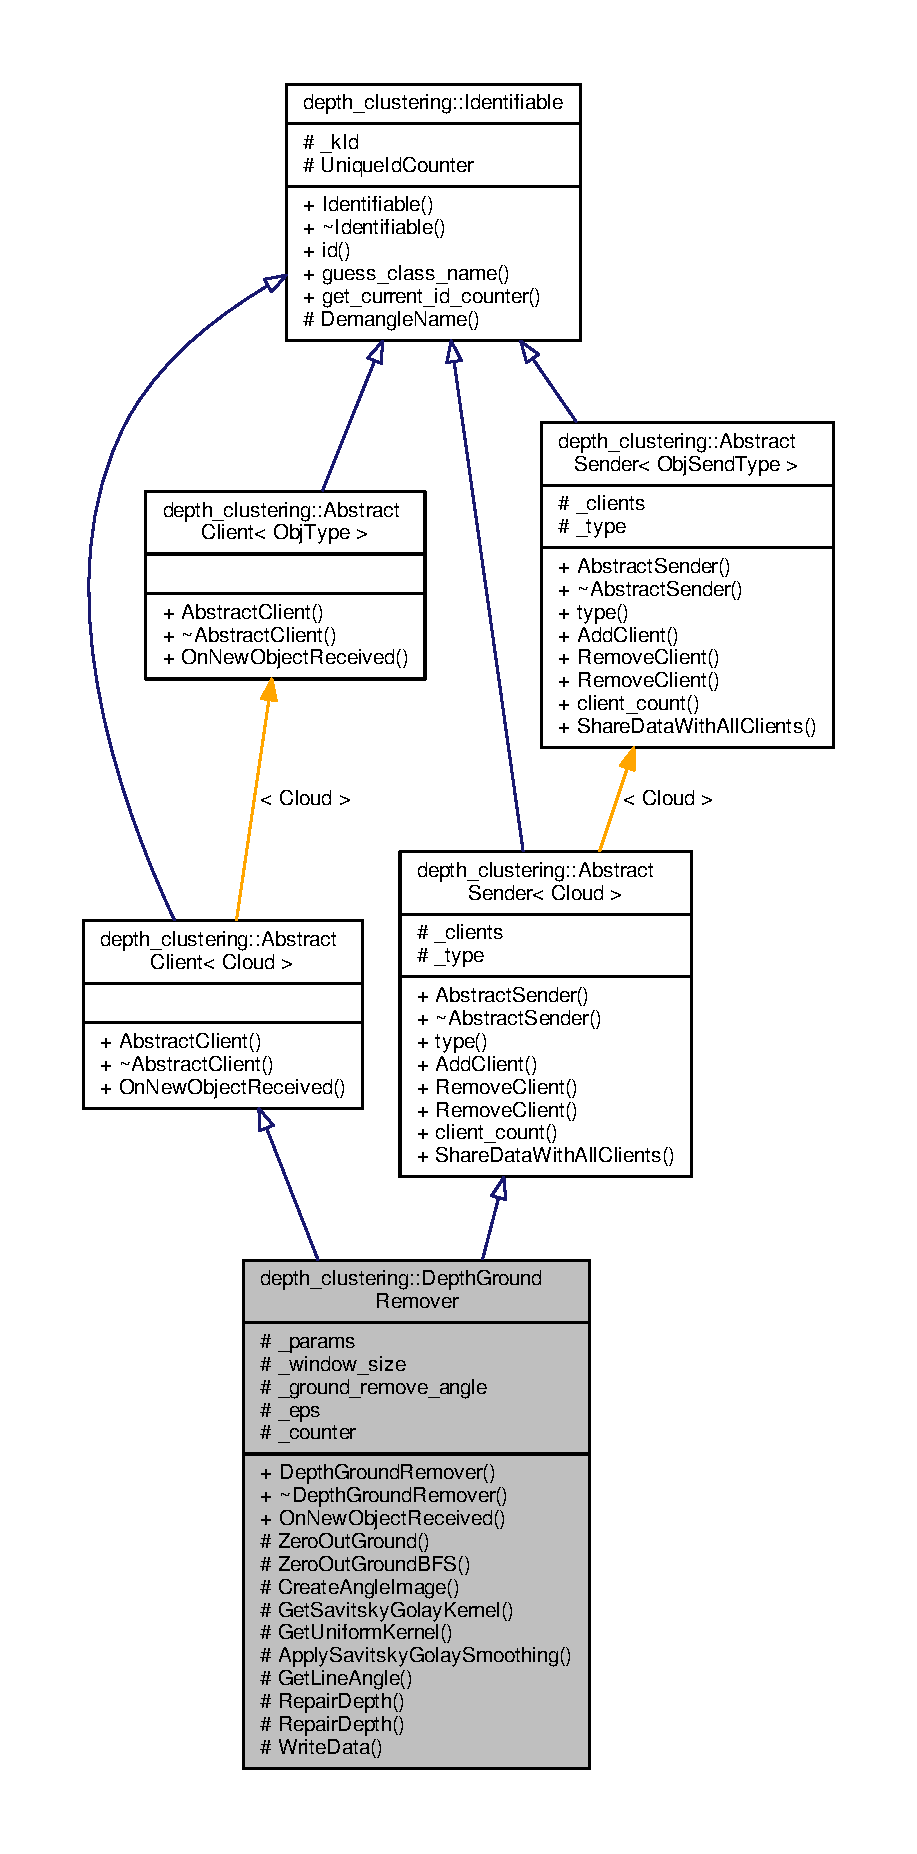
\includegraphics[height=550pt]{classdepth__clustering_1_1DepthGroundRemover__inherit__graph}
\end{center}
\end{figure}


Collaboration diagram for depth\-\_\-clustering\-:\-:Depth\-Ground\-Remover\-:
\nopagebreak
\begin{figure}[H]
\begin{center}
\leavevmode
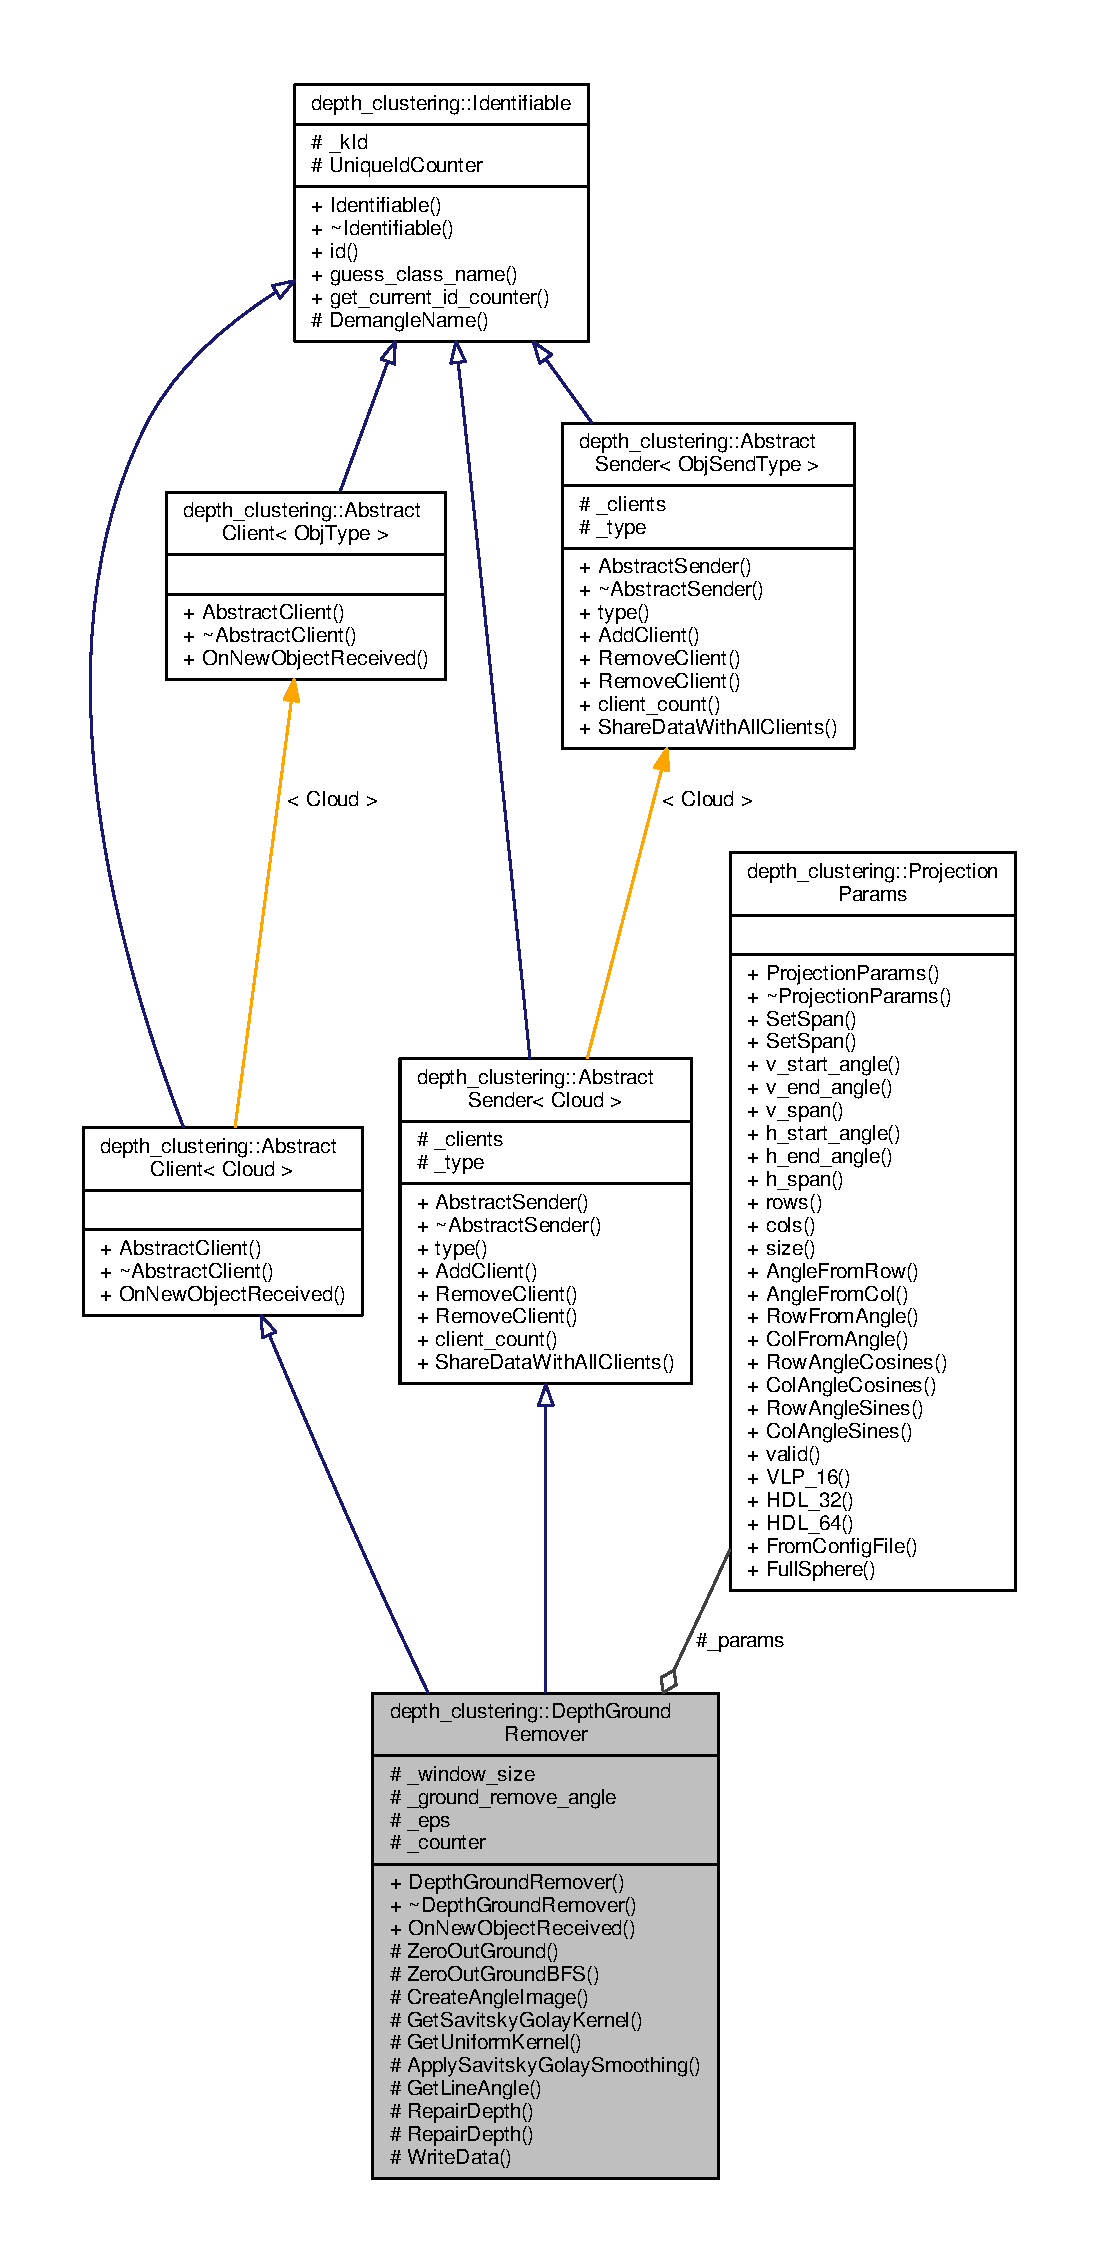
\includegraphics[height=550pt]{classdepth__clustering_1_1DepthGroundRemover__coll__graph}
\end{center}
\end{figure}


\subsection{Member Function Documentation}
\hypertarget{classdepth__clustering_1_1DepthGroundRemover_a63b32fa801a13021bf22699525579f8b}{\index{depth\-\_\-clustering\-::\-Depth\-Ground\-Remover@{depth\-\_\-clustering\-::\-Depth\-Ground\-Remover}!Apply\-Savitsky\-Golay\-Smoothing@{Apply\-Savitsky\-Golay\-Smoothing}}
\index{Apply\-Savitsky\-Golay\-Smoothing@{Apply\-Savitsky\-Golay\-Smoothing}!depth_clustering::DepthGroundRemover@{depth\-\_\-clustering\-::\-Depth\-Ground\-Remover}}
\subsubsection[{Apply\-Savitsky\-Golay\-Smoothing}]{\setlength{\rightskip}{0pt plus 5cm}Mat depth\-\_\-clustering\-::\-Depth\-Ground\-Remover\-::\-Apply\-Savitsky\-Golay\-Smoothing (
\begin{DoxyParamCaption}
\item[{const cv\-::\-Mat \&}]{column, }
\item[{int}]{window\-\_\-size}
\end{DoxyParamCaption}
)\hspace{0.3cm}{\ttfamily [protected]}}}\label{classdepth__clustering_1_1DepthGroundRemover_a63b32fa801a13021bf22699525579f8b}


Apply Savitsky-\/\-Golay smoothing to a column. 


\begin{DoxyParams}{Parameters}
{\em column} & \mbox{[}A column of an angle image\mbox{]} \\
\hline
\end{DoxyParams}
\begin{DoxyReturn}{Returns}
\mbox{[}a smoothed column\mbox{]} 
\end{DoxyReturn}
\hypertarget{classdepth__clustering_1_1DepthGroundRemover_af533c51a44aad9a56c12445b61b801b9}{\index{depth\-\_\-clustering\-::\-Depth\-Ground\-Remover@{depth\-\_\-clustering\-::\-Depth\-Ground\-Remover}!Create\-Angle\-Image@{Create\-Angle\-Image}}
\index{Create\-Angle\-Image@{Create\-Angle\-Image}!depth_clustering::DepthGroundRemover@{depth\-\_\-clustering\-::\-Depth\-Ground\-Remover}}
\subsubsection[{Create\-Angle\-Image}]{\setlength{\rightskip}{0pt plus 5cm}Mat depth\-\_\-clustering\-::\-Depth\-Ground\-Remover\-::\-Create\-Angle\-Image (
\begin{DoxyParamCaption}
\item[{const cv\-::\-Mat \&}]{depth\-\_\-image}
\end{DoxyParamCaption}
)\hspace{0.3cm}{\ttfamily [protected]}}}\label{classdepth__clustering_1_1DepthGroundRemover_af533c51a44aad9a56c12445b61b801b9}


create a help image with angle in radians written for each pixel 创建一个帮助图像,角度以弧度为单位编写像素 


\begin{DoxyParams}{Parameters}
{\em depth\-\_\-image} & \mbox{[}input depth image\mbox{]} \\
\hline
\end{DoxyParams}
\begin{DoxyReturn}{Returns}
\mbox{[}32 bit float image with angle in radians written in every pixel\mbox{]} 
\end{DoxyReturn}
\hypertarget{classdepth__clustering_1_1DepthGroundRemover_a29ba07a101794aab322ae3c0671806e0}{\index{depth\-\_\-clustering\-::\-Depth\-Ground\-Remover@{depth\-\_\-clustering\-::\-Depth\-Ground\-Remover}!Get\-Line\-Angle@{Get\-Line\-Angle}}
\index{Get\-Line\-Angle@{Get\-Line\-Angle}!depth_clustering::DepthGroundRemover@{depth\-\_\-clustering\-::\-Depth\-Ground\-Remover}}
\subsubsection[{Get\-Line\-Angle}]{\setlength{\rightskip}{0pt plus 5cm}Radians depth\-\_\-clustering\-::\-Depth\-Ground\-Remover\-::\-Get\-Line\-Angle (
\begin{DoxyParamCaption}
\item[{const cv\-::\-Mat \&}]{depth\-\_\-image, }
\item[{int}]{col, }
\item[{int}]{row\-\_\-curr, }
\item[{int}]{row\-\_\-neigh}
\end{DoxyParamCaption}
)\hspace{0.3cm}{\ttfamily [protected]}}}\label{classdepth__clustering_1_1DepthGroundRemover_a29ba07a101794aab322ae3c0671806e0}


Get line angle. 

Given two depth values and their angles compute the angle of the line that they spawn in the sensor frame.


\begin{DoxyParams}{Parameters}
{\em depth\-\_\-image} & \mbox{[}32 bit float image\mbox{]} \\
\hline
{\em col} & \mbox{[}current column\mbox{]} \\
\hline
{\em row\-\_\-curr} & \mbox{[}current row\mbox{]} \\
\hline
{\em row\-\_\-neigh} & \mbox{[}neighbor row\mbox{]} \\
\hline
\end{DoxyParams}
\begin{DoxyReturn}{Returns}
\mbox{[}angle of the line\mbox{]} 
\end{DoxyReturn}
\hypertarget{classdepth__clustering_1_1DepthGroundRemover_a8b660a1be94b529cf2554b8f72aee30d}{\index{depth\-\_\-clustering\-::\-Depth\-Ground\-Remover@{depth\-\_\-clustering\-::\-Depth\-Ground\-Remover}!Get\-Savitsky\-Golay\-Kernel@{Get\-Savitsky\-Golay\-Kernel}}
\index{Get\-Savitsky\-Golay\-Kernel@{Get\-Savitsky\-Golay\-Kernel}!depth_clustering::DepthGroundRemover@{depth\-\_\-clustering\-::\-Depth\-Ground\-Remover}}
\subsubsection[{Get\-Savitsky\-Golay\-Kernel}]{\setlength{\rightskip}{0pt plus 5cm}Mat depth\-\_\-clustering\-::\-Depth\-Ground\-Remover\-::\-Get\-Savitsky\-Golay\-Kernel (
\begin{DoxyParamCaption}
\item[{int}]{window\-\_\-size}
\end{DoxyParamCaption}
) const\hspace{0.3cm}{\ttfamily [protected]}}}\label{classdepth__clustering_1_1DepthGroundRemover_a8b660a1be94b529cf2554b8f72aee30d}


Get kernel for Savitsky-\/\-Golay filter为了 滤波器 

Get a column filter to process an image filled with data with Savitsky-\/\-Golay filter


\begin{DoxyParams}{Parameters}
{\em window\-\_\-size} & size of the kernel \\
\hline
\end{DoxyParams}
\begin{DoxyReturn}{Returns}
column Mat kernel 
\end{DoxyReturn}
\hypertarget{classdepth__clustering_1_1DepthGroundRemover_ab2c3bcc8df6cc70ad5057f5ec3bd074f}{\index{depth\-\_\-clustering\-::\-Depth\-Ground\-Remover@{depth\-\_\-clustering\-::\-Depth\-Ground\-Remover}!On\-New\-Object\-Received@{On\-New\-Object\-Received}}
\index{On\-New\-Object\-Received@{On\-New\-Object\-Received}!depth_clustering::DepthGroundRemover@{depth\-\_\-clustering\-::\-Depth\-Ground\-Remover}}
\subsubsection[{On\-New\-Object\-Received}]{\setlength{\rightskip}{0pt plus 5cm}void depth\-\_\-clustering\-::\-Depth\-Ground\-Remover\-::\-On\-New\-Object\-Received (
\begin{DoxyParamCaption}
\item[{const {\bf Cloud} \&}]{cloud, }
\item[{const int}]{sender\-\_\-id}
\end{DoxyParamCaption}
)\hspace{0.3cm}{\ttfamily [override]}, {\ttfamily [virtual]}}}\label{classdepth__clustering_1_1DepthGroundRemover_ab2c3bcc8df6cc70ad5057f5ec3bd074f}


when someone sends us an object we process it 

receiving a depth image we remove ground from it and send to next recepient 当接收到一个物体时我们首先对他们进行处理 然后把他发送给下一个接收者


\begin{DoxyParams}{Parameters}
{\em depth\-\_\-image} & 32 bit depth image 32位的深度图像 \\
\hline
{\em sender\-\_\-id} & id of the sender 传感器的\-I\-D 号 \\
\hline
\end{DoxyParams}


Implements \hyperlink{classdepth__clustering_1_1AbstractClient}{depth\-\_\-clustering\-::\-Abstract\-Client$<$ Cloud $>$}.

\hypertarget{classdepth__clustering_1_1DepthGroundRemover_a51dd313ed1bdda2188fb3a3fa1c5738e}{\index{depth\-\_\-clustering\-::\-Depth\-Ground\-Remover@{depth\-\_\-clustering\-::\-Depth\-Ground\-Remover}!Repair\-Depth@{Repair\-Depth}}
\index{Repair\-Depth@{Repair\-Depth}!depth_clustering::DepthGroundRemover@{depth\-\_\-clustering\-::\-Depth\-Ground\-Remover}}
\subsubsection[{Repair\-Depth}]{\setlength{\rightskip}{0pt plus 5cm}cv\-::\-Mat depth\-\_\-clustering\-::\-Depth\-Ground\-Remover\-::\-Repair\-Depth (
\begin{DoxyParamCaption}
\item[{const cv\-::\-Mat \&}]{no\-\_\-ground\-\_\-image, }
\item[{int}]{step, }
\item[{float}]{depth\-\_\-threshold}
\end{DoxyParamCaption}
)\hspace{0.3cm}{\ttfamily [protected]}}}\label{classdepth__clustering_1_1DepthGroundRemover_a51dd313ed1bdda2188fb3a3fa1c5738e}


Repair zeros in the depth image. 


\begin{DoxyParams}[1]{Parameters}
\mbox{\tt in}  & {\em depth\-\_\-image} & The depth image\\
\hline
\end{DoxyParams}
\begin{DoxyReturn}{Returns}
depth image with repaired values 
\end{DoxyReturn}
\hypertarget{classdepth__clustering_1_1DepthGroundRemover_a0f3733c1cbc915600d255246b1dccce0}{\index{depth\-\_\-clustering\-::\-Depth\-Ground\-Remover@{depth\-\_\-clustering\-::\-Depth\-Ground\-Remover}!Zero\-Out\-Ground@{Zero\-Out\-Ground}}
\index{Zero\-Out\-Ground@{Zero\-Out\-Ground}!depth_clustering::DepthGroundRemover@{depth\-\_\-clustering\-::\-Depth\-Ground\-Remover}}
\subsubsection[{Zero\-Out\-Ground}]{\setlength{\rightskip}{0pt plus 5cm}Mat depth\-\_\-clustering\-::\-Depth\-Ground\-Remover\-::\-Zero\-Out\-Ground (
\begin{DoxyParamCaption}
\item[{const cv\-::\-Mat \&}]{image, }
\item[{const cv\-::\-Mat \&}]{angle\-\_\-image, }
\item[{const Radians \&}]{threshold}
\end{DoxyParamCaption}
) const\hspace{0.3cm}{\ttfamily [protected]}}}\label{classdepth__clustering_1_1DepthGroundRemover_a0f3733c1cbc915600d255246b1dccce0}


Zero out all pixels that belong to ground 去除掉所有属于地面的点。 


\begin{DoxyParams}[1]{Parameters}
\mbox{\tt in}  & {\em image} & Input depth image 输入图像 \\
\hline
\mbox{\tt in}  & {\em angle\-\_\-image} & The angle image 角度图像 \\
\hline
\mbox{\tt in}  & {\em threshold} & angle threshold 角度阈值\\
\hline
\end{DoxyParams}
\begin{DoxyReturn}{Returns}
depth image with 0 instead of ground pixels 返回的图像中已经完全不含有地面上面的像素点了。 
\end{DoxyReturn}


The documentation for this class was generated from the following files\-:\begin{DoxyCompactItemize}
\item 
/home/hadoop/chy/depth\-\_\-clustering-\/master234/src/ground\-\_\-removal/depth\-\_\-ground\-\_\-remover.\-h\item 
/home/hadoop/chy/depth\-\_\-clustering-\/master234/src/ground\-\_\-removal/depth\-\_\-ground\-\_\-remover.\-cpp\end{DoxyCompactItemize}

\hypertarget{classdepth__clustering_1_1DijkstraImageLabeler}{\section{depth\-\_\-clustering\-:\-:Dijkstra\-Image\-Labeler$<$ S\-T\-E\-P\-\_\-\-R\-O\-W, S\-T\-E\-P\-\_\-\-C\-O\-L $>$ Class Template Reference}
\label{classdepth__clustering_1_1DijkstraImageLabeler}\index{depth\-\_\-clustering\-::\-Dijkstra\-Image\-Labeler$<$ S\-T\-E\-P\-\_\-\-R\-O\-W, S\-T\-E\-P\-\_\-\-C\-O\-L $>$@{depth\-\_\-clustering\-::\-Dijkstra\-Image\-Labeler$<$ S\-T\-E\-P\-\_\-\-R\-O\-W, S\-T\-E\-P\-\_\-\-C\-O\-L $>$}}
}


Label image with Dijkstra. Slower, then linear.  




{\ttfamily \#include $<$dijkstra\-\_\-image\-\_\-labeler.\-h$>$}

\subsection*{Public Member Functions}
\begin{DoxyCompactItemize}
\item 
\hypertarget{classdepth__clustering_1_1DijkstraImageLabeler_ac852e1ee20615b3ba62b31a090157cdd}{{\bfseries Dijkstra\-Image\-Labeler} (const cv\-::\-Mat \&depth\-\_\-image, const \hyperlink{classdepth__clustering_1_1ProjectionParams}{Projection\-Params} \&params, const Radians \&angle\-\_\-threshold)}\label{classdepth__clustering_1_1DijkstraImageLabeler_ac852e1ee20615b3ba62b31a090157cdd}

\item 
\hypertarget{classdepth__clustering_1_1DijkstraImageLabeler_a64086df9d6b682b13ef482b1cb2ea507}{void {\bfseries Compute\-Labels} () override}\label{classdepth__clustering_1_1DijkstraImageLabeler_a64086df9d6b682b13ef482b1cb2ea507}

\end{DoxyCompactItemize}
\subsection*{Public Attributes}
\begin{DoxyCompactItemize}
\item 
\hypertarget{classdepth__clustering_1_1DijkstraImageLabeler_ae7c58a8b42e1f17b76e3b48e610a1195}{std\-::array$<$ Pixel\-Coord, \\*
N\-E\-I\-G\-H\-\_\-\-S\-I\-Z\-E $>$ {\bfseries Neighborhood}}\label{classdepth__clustering_1_1DijkstraImageLabeler_ae7c58a8b42e1f17b76e3b48e610a1195}

\end{DoxyCompactItemize}
\subsection*{Static Public Attributes}
\begin{DoxyCompactItemize}
\item 
\hypertarget{classdepth__clustering_1_1DijkstraImageLabeler_a3a1f1c3b1eac8cb71ff04b9d6cc58ea3}{static constexpr int16\-\_\-t {\bfseries N\-E\-I\-G\-H\-\_\-\-S\-I\-Z\-E} = 2 $\ast$ S\-T\-E\-P\-\_\-\-R\-O\-W + 2 $\ast$ S\-T\-E\-P\-\_\-\-C\-O\-L}\label{classdepth__clustering_1_1DijkstraImageLabeler_a3a1f1c3b1eac8cb71ff04b9d6cc58ea3}

\end{DoxyCompactItemize}
\subsection*{Additional Inherited Members}


\subsection{Detailed Description}
\subsubsection*{template$<$int16\-\_\-t S\-T\-E\-P\-\_\-\-R\-O\-W = 1, int16\-\_\-t S\-T\-E\-P\-\_\-\-C\-O\-L = 1$>$class depth\-\_\-clustering\-::\-Dijkstra\-Image\-Labeler$<$ S\-T\-E\-P\-\_\-\-R\-O\-W, S\-T\-E\-P\-\_\-\-C\-O\-L $>$}

Label image with Dijkstra. Slower, then linear. 

Inheritance diagram for depth\-\_\-clustering\-:\-:Dijkstra\-Image\-Labeler$<$ S\-T\-E\-P\-\_\-\-R\-O\-W, S\-T\-E\-P\-\_\-\-C\-O\-L $>$\-:
\nopagebreak
\begin{figure}[H]
\begin{center}
\leavevmode
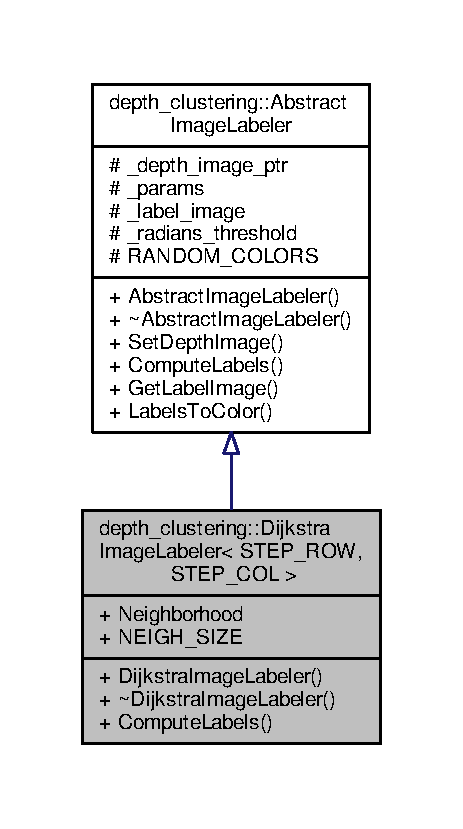
\includegraphics[width=222pt]{classdepth__clustering_1_1DijkstraImageLabeler__inherit__graph}
\end{center}
\end{figure}


Collaboration diagram for depth\-\_\-clustering\-:\-:Dijkstra\-Image\-Labeler$<$ S\-T\-E\-P\-\_\-\-R\-O\-W, S\-T\-E\-P\-\_\-\-C\-O\-L $>$\-:
\nopagebreak
\begin{figure}[H]
\begin{center}
\leavevmode
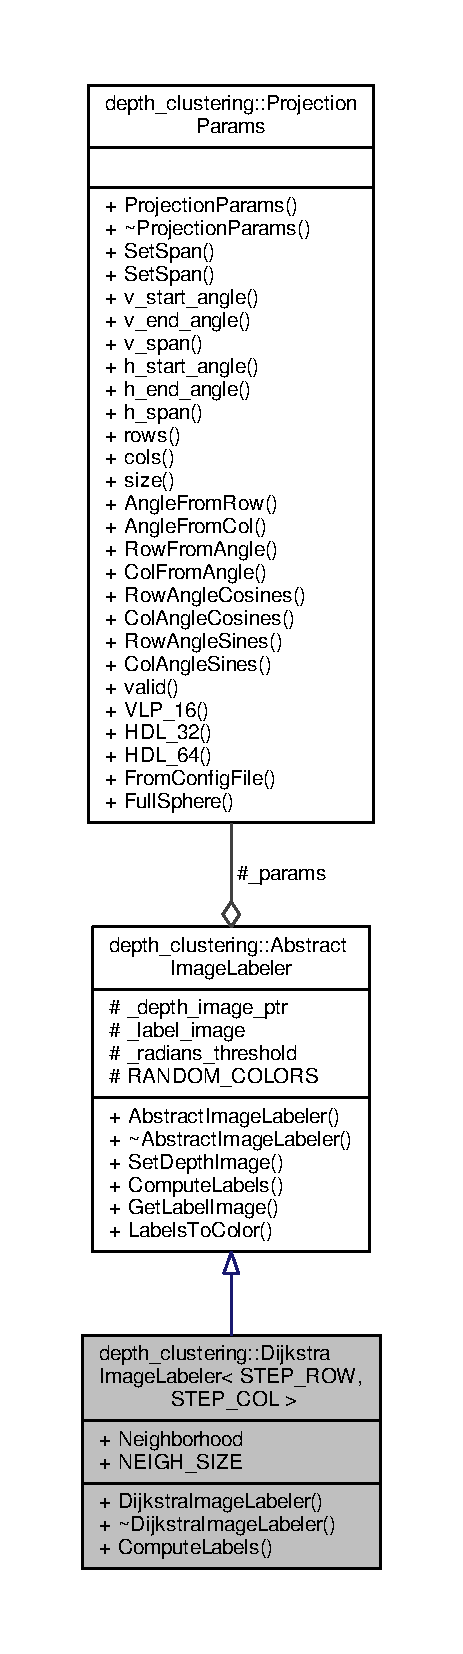
\includegraphics[height=550pt]{classdepth__clustering_1_1DijkstraImageLabeler__coll__graph}
\end{center}
\end{figure}


The documentation for this class was generated from the following file\-:\begin{DoxyCompactItemize}
\item 
/home/hadoop/chy/depth\-\_\-clustering-\/master234/src/image\-\_\-labelers/dijkstra\-\_\-image\-\_\-labeler.\-h\end{DoxyCompactItemize}

\hypertarget{classdepth__clustering_1_1EuclideanClusterer}{\section{depth\-\_\-clustering\-:\-:Euclidean\-Clusterer Class Reference}
\label{classdepth__clustering_1_1EuclideanClusterer}\index{depth\-\_\-clustering\-::\-Euclidean\-Clusterer@{depth\-\_\-clustering\-::\-Euclidean\-Clusterer}}
}


Class for euclidean clustering.  




{\ttfamily \#include $<$euclidean\-\_\-clusterer.\-h$>$}

\subsection*{Public Types}
\begin{DoxyCompactItemize}
\item 
\hypertarget{classdepth__clustering_1_1EuclideanClusterer_a7c8df2531faab16c7156087cd62d31ca}{using {\bfseries Point\-T} = pcl\-::\-Point\-X\-Y\-Z\-L}\label{classdepth__clustering_1_1EuclideanClusterer_a7c8df2531faab16c7156087cd62d31ca}

\end{DoxyCompactItemize}
\subsection*{Public Member Functions}
\begin{DoxyCompactItemize}
\item 
\hypertarget{classdepth__clustering_1_1EuclideanClusterer_a1c8b10d1977bf4c1f463d2f1942526df}{{\bfseries Euclidean\-Clusterer} (double cluster\-\_\-tollerance=0.\-2, uint16\-\_\-t min\-\_\-cluster\-\_\-size=100, uint16\-\_\-t max\-\_\-cluster\-\_\-size=25000, uint16\-\_\-t skip=10)}\label{classdepth__clustering_1_1EuclideanClusterer_a1c8b10d1977bf4c1f463d2f1942526df}

\item 
void \hyperlink{classdepth__clustering_1_1EuclideanClusterer_a8ebdd098c514a05f17f16070255b27a6}{On\-New\-Object\-Received} (const \hyperlink{classdepth__clustering_1_1Cloud}{Cloud} \&cloud, const int sender\-\_\-id) override
\begin{DoxyCompactList}\small\item\em Gets called when somebody sends this client an object. \end{DoxyCompactList}\end{DoxyCompactItemize}
\subsection*{Additional Inherited Members}


\subsection{Detailed Description}
Class for euclidean clustering. 

Inheritance diagram for depth\-\_\-clustering\-:\-:Euclidean\-Clusterer\-:
\nopagebreak
\begin{figure}[H]
\begin{center}
\leavevmode
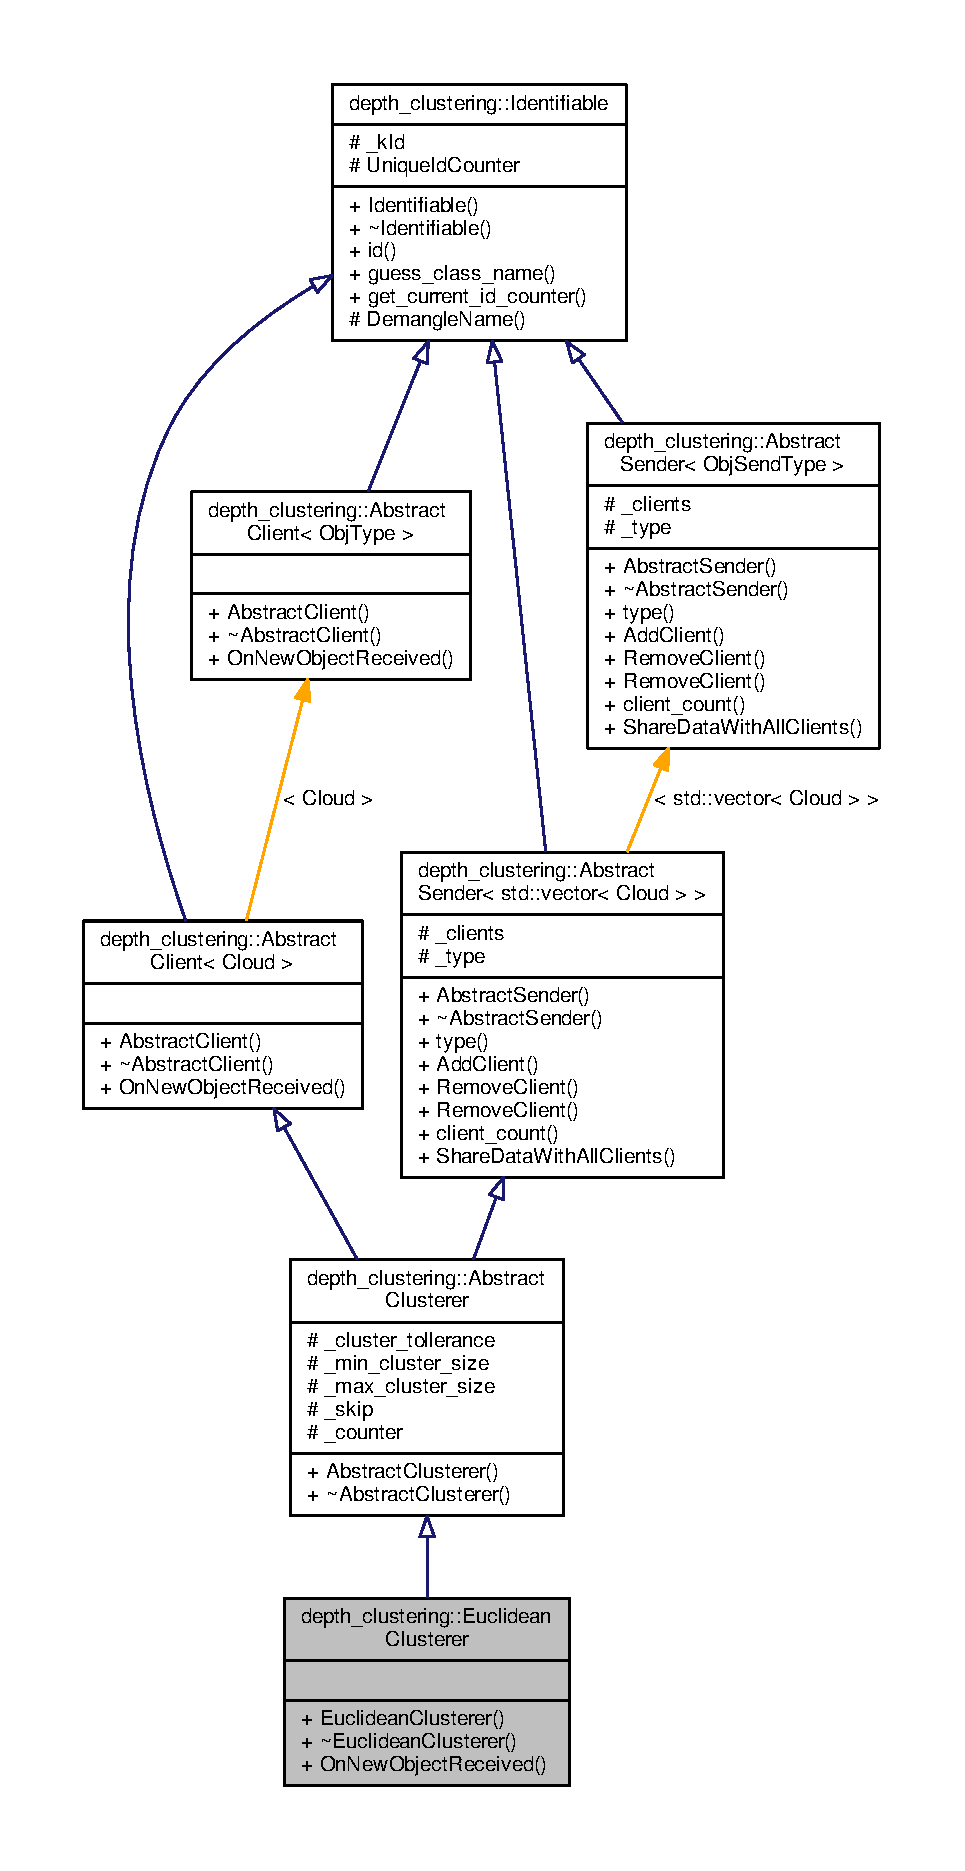
\includegraphics[height=550pt]{classdepth__clustering_1_1EuclideanClusterer__inherit__graph}
\end{center}
\end{figure}


Collaboration diagram for depth\-\_\-clustering\-:\-:Euclidean\-Clusterer\-:
\nopagebreak
\begin{figure}[H]
\begin{center}
\leavevmode
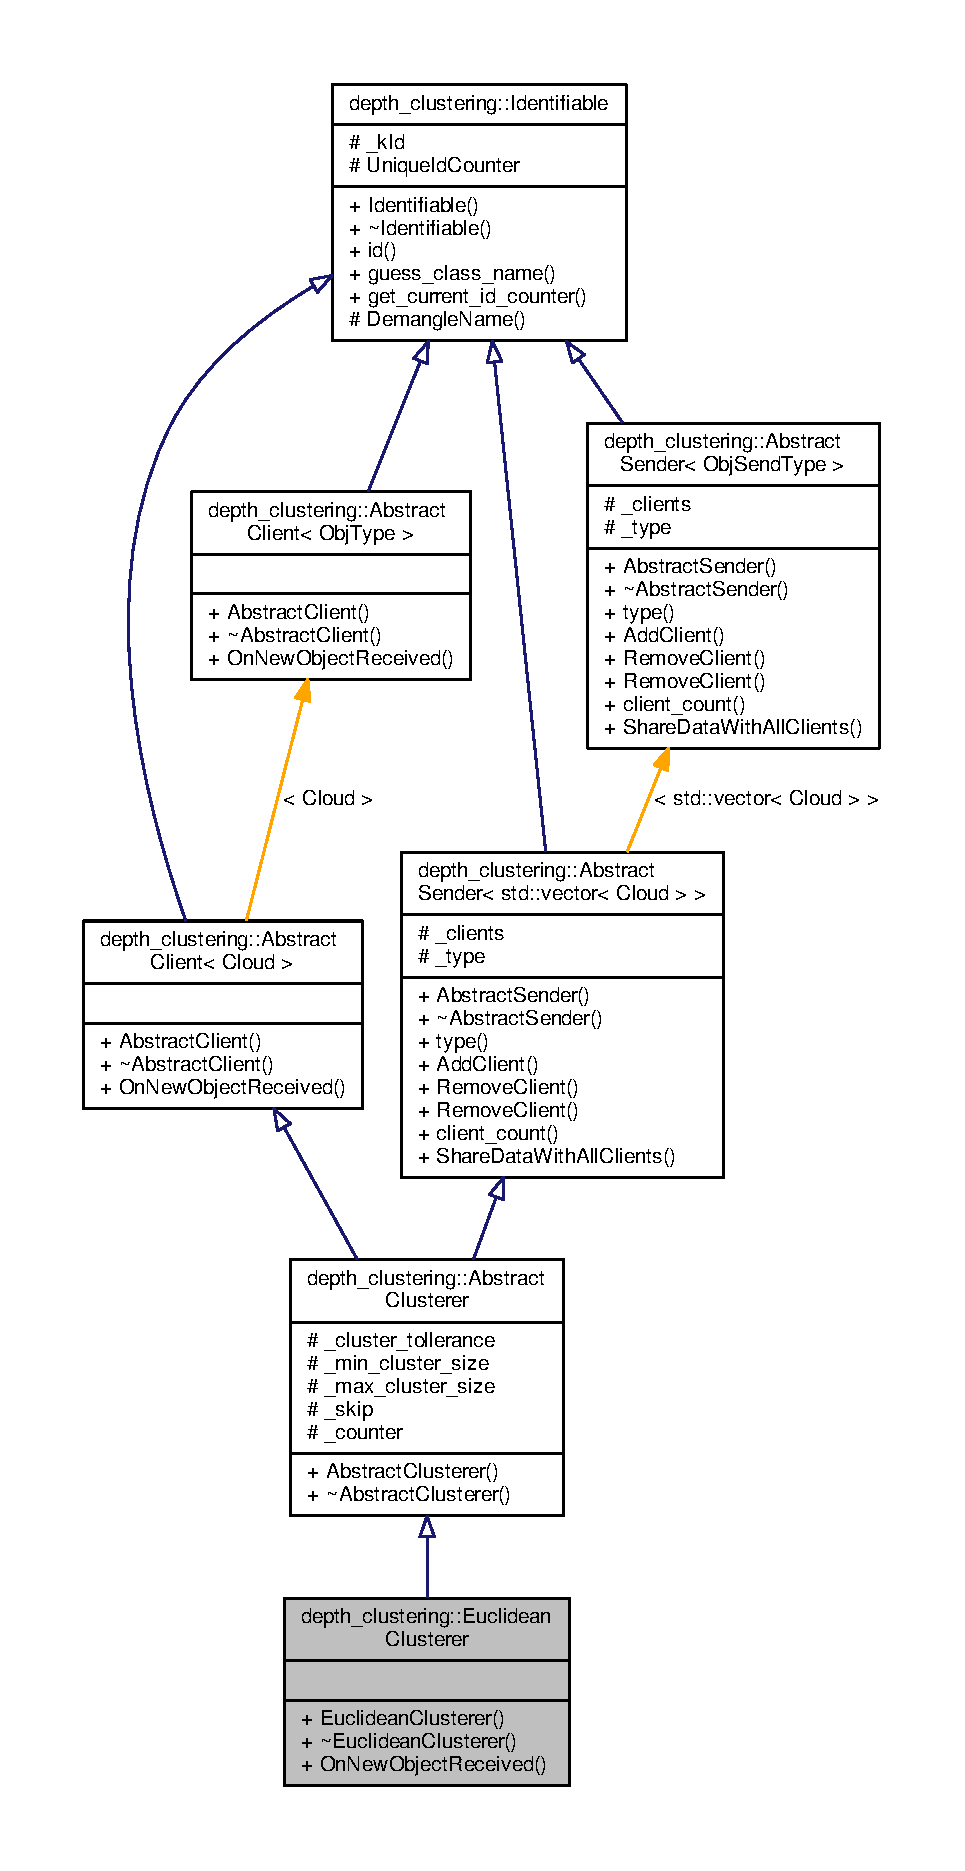
\includegraphics[height=550pt]{classdepth__clustering_1_1EuclideanClusterer__coll__graph}
\end{center}
\end{figure}


\subsection{Member Function Documentation}
\hypertarget{classdepth__clustering_1_1EuclideanClusterer_a8ebdd098c514a05f17f16070255b27a6}{\index{depth\-\_\-clustering\-::\-Euclidean\-Clusterer@{depth\-\_\-clustering\-::\-Euclidean\-Clusterer}!On\-New\-Object\-Received@{On\-New\-Object\-Received}}
\index{On\-New\-Object\-Received@{On\-New\-Object\-Received}!depth_clustering::EuclideanClusterer@{depth\-\_\-clustering\-::\-Euclidean\-Clusterer}}
\subsubsection[{On\-New\-Object\-Received}]{\setlength{\rightskip}{0pt plus 5cm}void depth\-\_\-clustering\-::\-Euclidean\-Clusterer\-::\-On\-New\-Object\-Received (
\begin{DoxyParamCaption}
\item[{const {\bf Cloud} \&}]{cloud, }
\item[{const int}]{sender\-\_\-id}
\end{DoxyParamCaption}
)\hspace{0.3cm}{\ttfamily [inline]}, {\ttfamily [override]}, {\ttfamily [virtual]}}}\label{classdepth__clustering_1_1EuclideanClusterer_a8ebdd098c514a05f17f16070255b27a6}


Gets called when somebody sends this client an object. 


\begin{DoxyParams}[1]{Parameters}
\mbox{\tt in}  & {\em cloud} & The cloud to cluster \\
\hline
\mbox{\tt in}  & {\em sender\-\_\-id} & The sender identifier \\
\hline
\end{DoxyParams}


Implements \hyperlink{classdepth__clustering_1_1AbstractClient}{depth\-\_\-clustering\-::\-Abstract\-Client$<$ Cloud $>$}.



Here is the call graph for this function\-:
\nopagebreak
\begin{figure}[H]
\begin{center}
\leavevmode
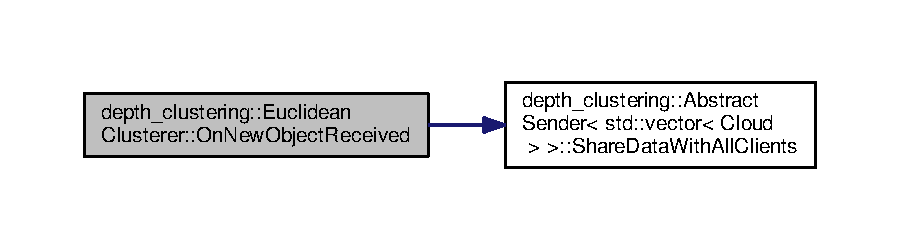
\includegraphics[width=350pt]{classdepth__clustering_1_1EuclideanClusterer_a8ebdd098c514a05f17f16070255b27a6_cgraph}
\end{center}
\end{figure}




The documentation for this class was generated from the following file\-:\begin{DoxyCompactItemize}
\item 
/home/hadoop/chy/depth\-\_\-clustering-\/master234/src/clusterers/euclidean\-\_\-clusterer.\-h\end{DoxyCompactItemize}

\hypertarget{classdepth__clustering_1_1FolderReader}{\section{depth\-\_\-clustering\-:\-:Folder\-Reader Class Reference}
\label{classdepth__clustering_1_1FolderReader}\index{depth\-\_\-clustering\-::\-Folder\-Reader@{depth\-\_\-clustering\-::\-Folder\-Reader}}
}


Reads a folder and can sort the inputs. Not too efficient.  




{\ttfamily \#include $<$folder\-\_\-reader.\-h$>$}

\subsection*{Public Types}
\begin{DoxyCompactItemize}
\item 
enum {\bfseries Order} \{ {\bfseries S\-O\-R\-T\-E\-D}, 
{\bfseries U\-N\-D\-E\-F\-I\-N\-E\-D}
 \}
\end{DoxyCompactItemize}
\subsection*{Public Member Functions}
\begin{DoxyCompactItemize}
\item 
\hypertarget{classdepth__clustering_1_1FolderReader_a80ae7f477c0ba4ca20e58e0eff0874b2}{{\bfseries Folder\-Reader} (const std\-::string \&folder\-\_\-path, const std\-::string \&ending\-\_\-with, const Order order=Order\-::\-U\-N\-D\-E\-F\-I\-N\-E\-D)}\label{classdepth__clustering_1_1FolderReader_a80ae7f477c0ba4ca20e58e0eff0874b2}

\item 
\hypertarget{classdepth__clustering_1_1FolderReader_a298f7b246759d1d926746e057c9d96a0}{{\bfseries Folder\-Reader} (const std\-::string \&folder\-\_\-path, const std\-::string \&starting\-\_\-with, const std\-::string \&ending\-\_\-with, const Order order=Order\-::\-U\-N\-D\-E\-F\-I\-N\-E\-D)}\label{classdepth__clustering_1_1FolderReader_a298f7b246759d1d926746e057c9d96a0}

\item 
\hypertarget{classdepth__clustering_1_1FolderReader_aeb4575a662afa48264fec96f4802db90}{std\-::string {\bfseries Get\-Next\-File\-Path} ()}\label{classdepth__clustering_1_1FolderReader_aeb4575a662afa48264fec96f4802db90}

\item 
\hypertarget{classdepth__clustering_1_1FolderReader_a416eee1780485b6d677488d3e44014d0}{const std\-::vector$<$ std\-::string $>$ \& {\bfseries Get\-All\-File\-Paths} () const }\label{classdepth__clustering_1_1FolderReader_a416eee1780485b6d677488d3e44014d0}

\end{DoxyCompactItemize}
\subsection*{Protected Attributes}
\begin{DoxyCompactItemize}
\item 
\hypertarget{classdepth__clustering_1_1FolderReader_af9ed4e41e57050d7859cd066eb841792}{std\-::vector$<$ std\-::string $>$ {\bfseries \-\_\-all\-\_\-paths}}\label{classdepth__clustering_1_1FolderReader_af9ed4e41e57050d7859cd066eb841792}

\item 
\hypertarget{classdepth__clustering_1_1FolderReader_aa9fae723281ea00040a803fc15a86d5d}{size\-\_\-t {\bfseries \-\_\-path\-\_\-counter}}\label{classdepth__clustering_1_1FolderReader_aa9fae723281ea00040a803fc15a86d5d}

\end{DoxyCompactItemize}


\subsection{Detailed Description}
Reads a folder and can sort the inputs. Not too efficient. 

Collaboration diagram for depth\-\_\-clustering\-:\-:Folder\-Reader\-:
\nopagebreak
\begin{figure}[H]
\begin{center}
\leavevmode
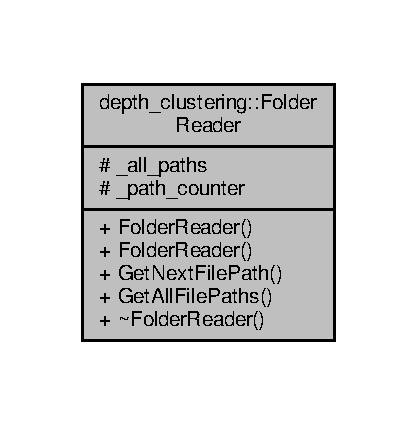
\includegraphics[width=200pt]{classdepth__clustering_1_1FolderReader__coll__graph}
\end{center}
\end{figure}


The documentation for this class was generated from the following files\-:\begin{DoxyCompactItemize}
\item 
/home/hadoop/chy/depth\-\_\-clustering-\/master234/src/utils/folder\-\_\-reader.\-h\item 
/home/hadoop/chy/depth\-\_\-clustering-\/master234/src/utils/folder\-\_\-reader.\-cpp\end{DoxyCompactItemize}

\hypertarget{classdepth__clustering_1_1Identifiable}{\section{depth\-\_\-clustering\-:\-:Identifiable Class Reference}
\label{classdepth__clustering_1_1Identifiable}\index{depth\-\_\-clustering\-::\-Identifiable@{depth\-\_\-clustering\-::\-Identifiable}}
}


Class for identifiable.  




{\ttfamily \#include $<$identifiable.\-h$>$}

\subsection*{Public Member Functions}
\begin{DoxyCompactItemize}
\item 
int \hyperlink{classdepth__clustering_1_1Identifiable_a020b49a5102a2ef0eec7b9e74add7669}{id} () const 
\begin{DoxyCompactList}\small\item\em Gets current object id. \end{DoxyCompactList}\item 
virtual std\-::string \hyperlink{classdepth__clustering_1_1Identifiable_af6769d100c7e7932b71a7f83ce6eafcc}{guess\-\_\-class\-\_\-name} () const 
\begin{DoxyCompactList}\small\item\em Guesses class name from typeid. \end{DoxyCompactList}\end{DoxyCompactItemize}
\subsection*{Static Public Member Functions}
\begin{DoxyCompactItemize}
\item 
static int \hyperlink{classdepth__clustering_1_1Identifiable_a7b3be5250a82404765617ba7239041f1}{get\-\_\-current\-\_\-id\-\_\-counter} ()
\begin{DoxyCompactList}\small\item\em Gets the current identifier counter. \end{DoxyCompactList}\end{DoxyCompactItemize}
\subsection*{Static Protected Member Functions}
\begin{DoxyCompactItemize}
\item 
\hypertarget{classdepth__clustering_1_1Identifiable_a61d070e7b5adbef771d5b4df7b9e2f75}{static std\-::string {\bfseries Demangle\-Name} (const char $\ast$tname)}\label{classdepth__clustering_1_1Identifiable_a61d070e7b5adbef771d5b4df7b9e2f75}

\end{DoxyCompactItemize}
\subsection*{Protected Attributes}
\begin{DoxyCompactItemize}
\item 
\hypertarget{classdepth__clustering_1_1Identifiable_a82e9edccdd02896f9bcd2fa829645158}{const int {\bfseries \-\_\-k\-Id}}\label{classdepth__clustering_1_1Identifiable_a82e9edccdd02896f9bcd2fa829645158}

\end{DoxyCompactItemize}
\subsection*{Static Protected Attributes}
\begin{DoxyCompactItemize}
\item 
\hypertarget{classdepth__clustering_1_1Identifiable_ac467cc001b2e67e09a10c7dc0da96c4c}{static int {\bfseries Unique\-Id\-Counter} = 0}\label{classdepth__clustering_1_1Identifiable_ac467cc001b2e67e09a10c7dc0da96c4c}

\end{DoxyCompactItemize}


\subsection{Detailed Description}
Class for identifiable. 

Inheritance diagram for depth\-\_\-clustering\-:\-:Identifiable\-:
\nopagebreak
\begin{figure}[H]
\begin{center}
\leavevmode
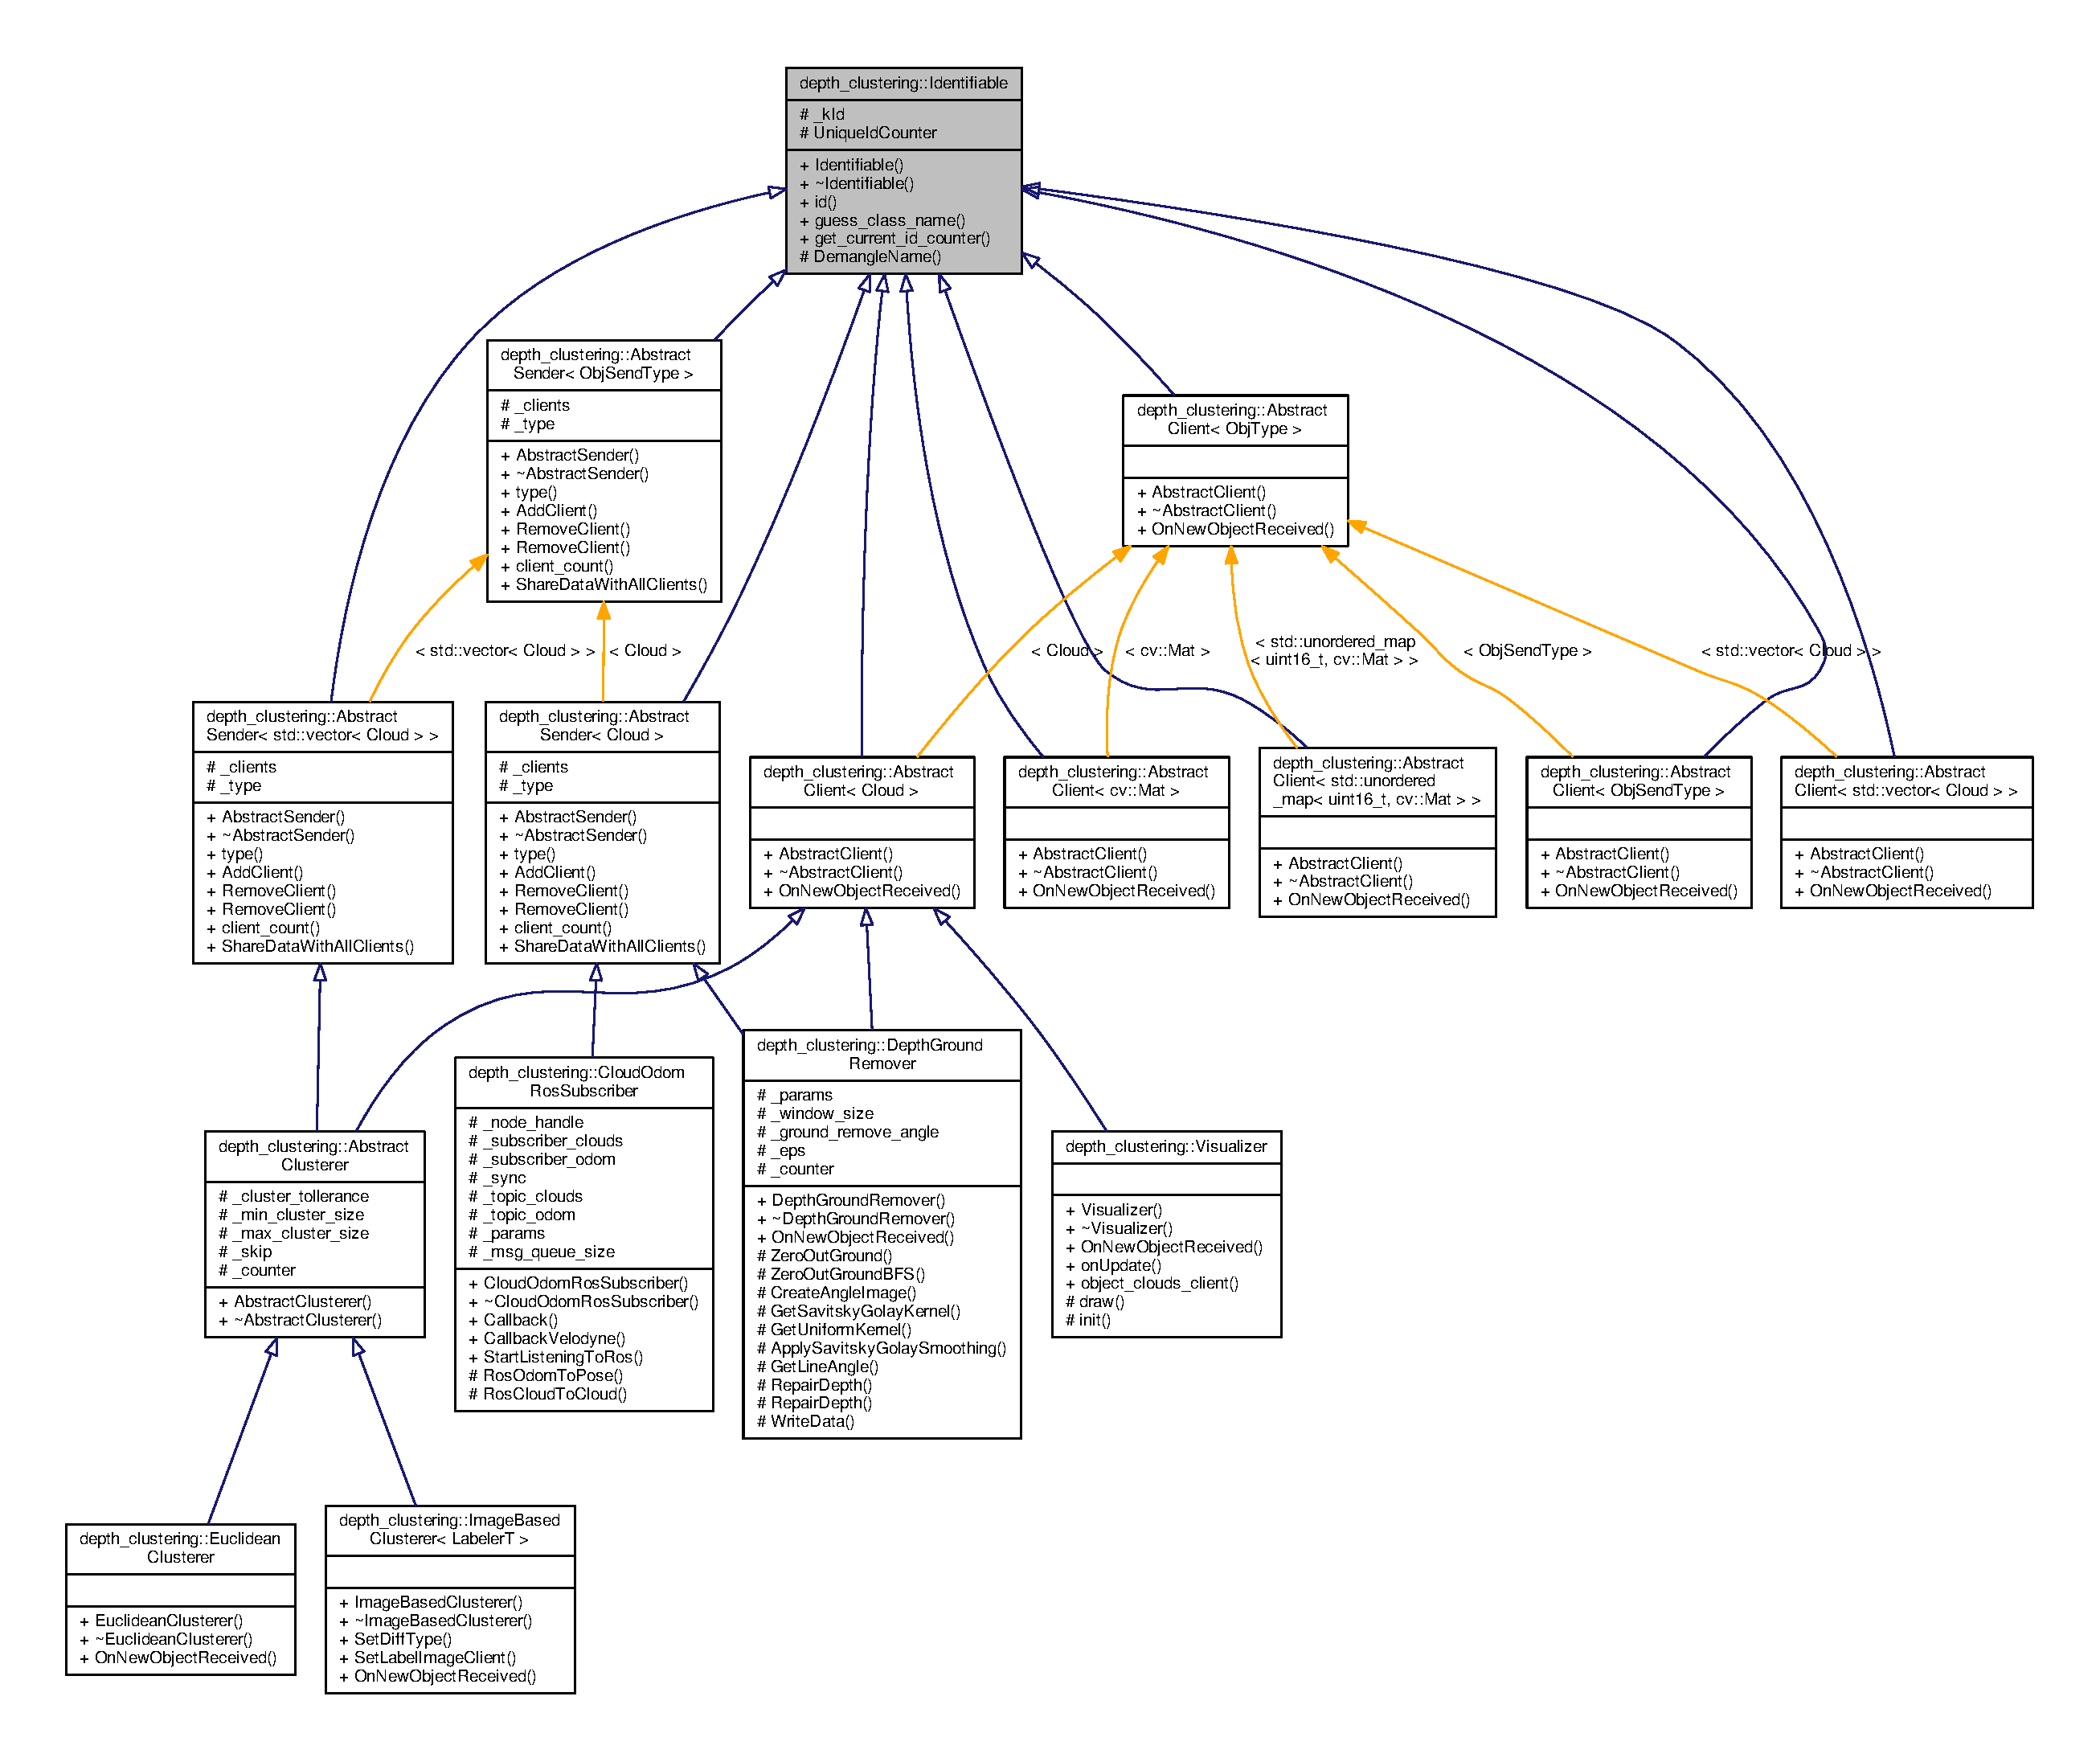
\includegraphics[width=350pt]{classdepth__clustering_1_1Identifiable__inherit__graph}
\end{center}
\end{figure}


Collaboration diagram for depth\-\_\-clustering\-:\-:Identifiable\-:
\nopagebreak
\begin{figure}[H]
\begin{center}
\leavevmode
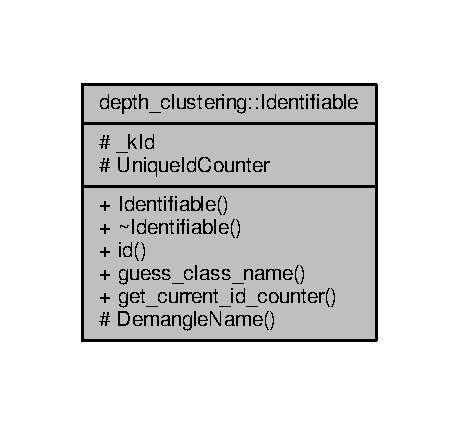
\includegraphics[width=220pt]{classdepth__clustering_1_1Identifiable__coll__graph}
\end{center}
\end{figure}


\subsection{Member Function Documentation}
\hypertarget{classdepth__clustering_1_1Identifiable_a7b3be5250a82404765617ba7239041f1}{\index{depth\-\_\-clustering\-::\-Identifiable@{depth\-\_\-clustering\-::\-Identifiable}!get\-\_\-current\-\_\-id\-\_\-counter@{get\-\_\-current\-\_\-id\-\_\-counter}}
\index{get\-\_\-current\-\_\-id\-\_\-counter@{get\-\_\-current\-\_\-id\-\_\-counter}!depth_clustering::Identifiable@{depth\-\_\-clustering\-::\-Identifiable}}
\subsubsection[{get\-\_\-current\-\_\-id\-\_\-counter}]{\setlength{\rightskip}{0pt plus 5cm}static int depth\-\_\-clustering\-::\-Identifiable\-::get\-\_\-current\-\_\-id\-\_\-counter (
\begin{DoxyParamCaption}
{}
\end{DoxyParamCaption}
)\hspace{0.3cm}{\ttfamily [inline]}, {\ttfamily [static]}}}\label{classdepth__clustering_1_1Identifiable_a7b3be5250a82404765617ba7239041f1}


Gets the current identifier counter. 

\begin{DoxyReturn}{Returns}
The current identifier counter. 
\end{DoxyReturn}
\hypertarget{classdepth__clustering_1_1Identifiable_af6769d100c7e7932b71a7f83ce6eafcc}{\index{depth\-\_\-clustering\-::\-Identifiable@{depth\-\_\-clustering\-::\-Identifiable}!guess\-\_\-class\-\_\-name@{guess\-\_\-class\-\_\-name}}
\index{guess\-\_\-class\-\_\-name@{guess\-\_\-class\-\_\-name}!depth_clustering::Identifiable@{depth\-\_\-clustering\-::\-Identifiable}}
\subsubsection[{guess\-\_\-class\-\_\-name}]{\setlength{\rightskip}{0pt plus 5cm}virtual std\-::string depth\-\_\-clustering\-::\-Identifiable\-::guess\-\_\-class\-\_\-name (
\begin{DoxyParamCaption}
{}
\end{DoxyParamCaption}
) const\hspace{0.3cm}{\ttfamily [inline]}, {\ttfamily [virtual]}}}\label{classdepth__clustering_1_1Identifiable_af6769d100c7e7932b71a7f83ce6eafcc}


Guesses class name from typeid. 

\begin{DoxyReturn}{Returns}
Class name as string. 
\end{DoxyReturn}


Here is the caller graph for this function\-:
\nopagebreak
\begin{figure}[H]
\begin{center}
\leavevmode
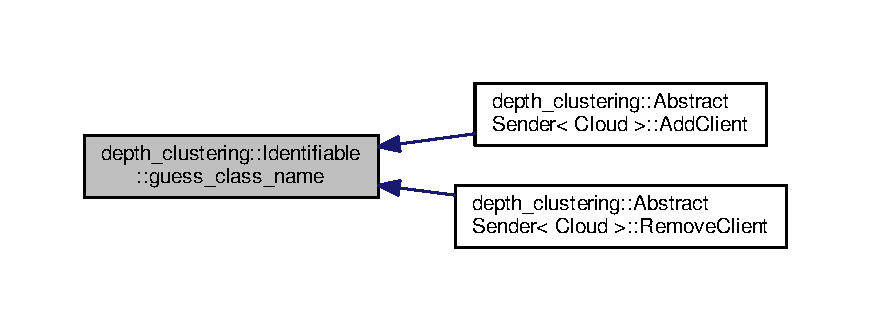
\includegraphics[width=350pt]{classdepth__clustering_1_1Identifiable_af6769d100c7e7932b71a7f83ce6eafcc_icgraph}
\end{center}
\end{figure}


\hypertarget{classdepth__clustering_1_1Identifiable_a020b49a5102a2ef0eec7b9e74add7669}{\index{depth\-\_\-clustering\-::\-Identifiable@{depth\-\_\-clustering\-::\-Identifiable}!id@{id}}
\index{id@{id}!depth_clustering::Identifiable@{depth\-\_\-clustering\-::\-Identifiable}}
\subsubsection[{id}]{\setlength{\rightskip}{0pt plus 5cm}int depth\-\_\-clustering\-::\-Identifiable\-::id (
\begin{DoxyParamCaption}
{}
\end{DoxyParamCaption}
) const\hspace{0.3cm}{\ttfamily [inline]}}}\label{classdepth__clustering_1_1Identifiable_a020b49a5102a2ef0eec7b9e74add7669}


Gets current object id. 

\begin{DoxyReturn}{Returns}
id of the object. 
\end{DoxyReturn}


Here is the caller graph for this function\-:
\nopagebreak
\begin{figure}[H]
\begin{center}
\leavevmode
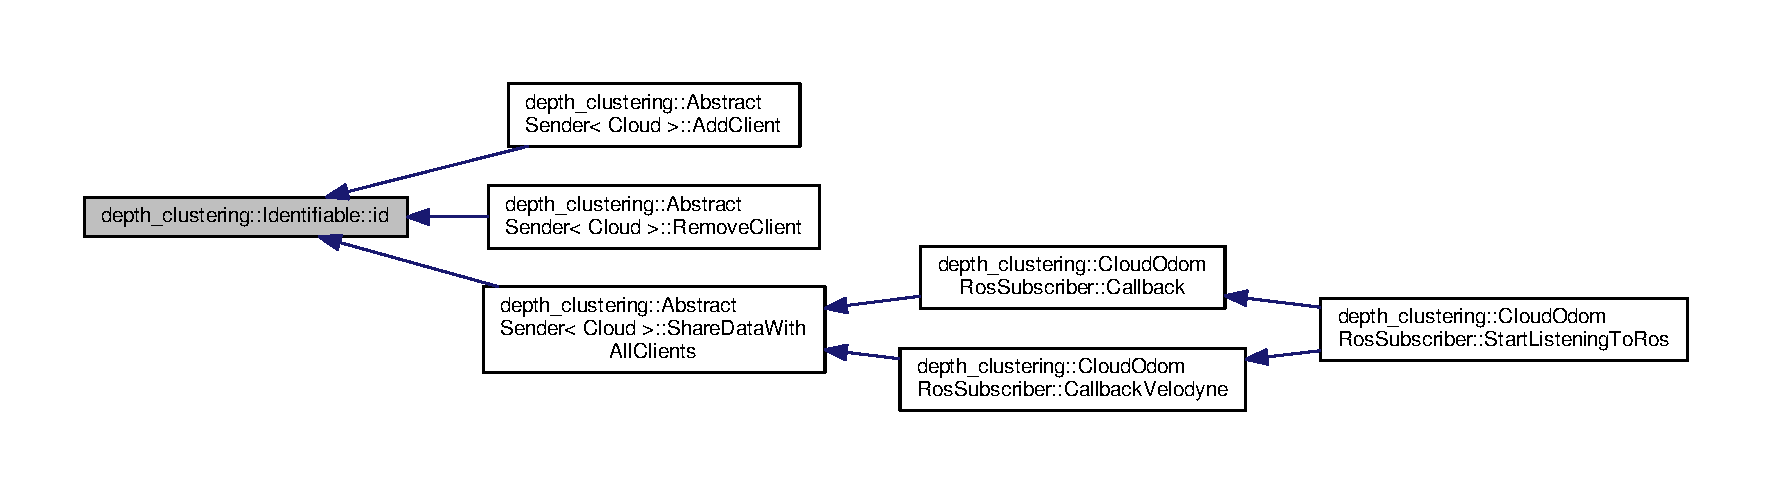
\includegraphics[width=350pt]{classdepth__clustering_1_1Identifiable_a020b49a5102a2ef0eec7b9e74add7669_icgraph}
\end{center}
\end{figure}




The documentation for this class was generated from the following files\-:\begin{DoxyCompactItemize}
\item 
/home/hadoop/chy/depth\-\_\-clustering-\/master234/src/communication/identifiable.\-h\item 
/home/hadoop/chy/depth\-\_\-clustering-\/master234/src/communication/identifiable.\-cpp\end{DoxyCompactItemize}

\hypertarget{classdepth__clustering_1_1ImageBasedClusterer}{\section{depth\-\_\-clustering\-:\-:Image\-Based\-Clusterer$<$ Labeler\-T $>$ Class Template Reference}
\label{classdepth__clustering_1_1ImageBasedClusterer}\index{depth\-\_\-clustering\-::\-Image\-Based\-Clusterer$<$ Labeler\-T $>$@{depth\-\_\-clustering\-::\-Image\-Based\-Clusterer$<$ Labeler\-T $>$}}
}


Class for image based clusterer.  




{\ttfamily \#include $<$image\-\_\-based\-\_\-clusterer.\-h$>$}

\subsection*{Public Types}
\begin{DoxyCompactItemize}
\item 
\hypertarget{classdepth__clustering_1_1ImageBasedClusterer_a62774a9ad3f50dd9811c2194c99eff7f}{using {\bfseries Receiver} = \hyperlink{classdepth__clustering_1_1AbstractClient}{Abstract\-Client}$<$ \hyperlink{classdepth__clustering_1_1Cloud}{Cloud} $>$}\label{classdepth__clustering_1_1ImageBasedClusterer_a62774a9ad3f50dd9811c2194c99eff7f}

\item 
\hypertarget{classdepth__clustering_1_1ImageBasedClusterer_a639353b7fb8f37636bf38aa371c2a7ec}{using {\bfseries Sender} = \hyperlink{classdepth__clustering_1_1AbstractSender}{Abstract\-Sender}$<$ std\-::vector$<$ \hyperlink{classdepth__clustering_1_1Cloud}{Cloud} $>$$>$}\label{classdepth__clustering_1_1ImageBasedClusterer_a639353b7fb8f37636bf38aa371c2a7ec}

\end{DoxyCompactItemize}
\subsection*{Public Member Functions}
\begin{DoxyCompactItemize}
\item 
\hyperlink{classdepth__clustering_1_1ImageBasedClusterer_a6a8bdd77542e14ee420988ad80579f35}{Image\-Based\-Clusterer} (Radians angle\-\_\-tollerance=8\-\_\-deg, uint16\-\_\-t min\-\_\-cluster\-\_\-size=100, uint16\-\_\-t max\-\_\-cluster\-\_\-size=25000)
\begin{DoxyCompactList}\small\item\em Construct an image-\/based clusterer. \end{DoxyCompactList}\item 
void \hyperlink{classdepth__clustering_1_1ImageBasedClusterer_a0dd114829041816d309d6c8f9ff41cad}{Set\-Diff\-Type} (Diff\-Factory\-::\-Diff\-Type diff\-\_\-type)
\begin{DoxyCompactList}\small\item\em Sets the difference type. \end{DoxyCompactList}\item 
void \hyperlink{classdepth__clustering_1_1ImageBasedClusterer_a6af0de0dad7450c34c655fb447886716}{Set\-Label\-Image\-Client} (\hyperlink{classdepth__clustering_1_1AbstractClient}{Abstract\-Client}$<$ cv\-::\-Mat $>$ $\ast$client)
\begin{DoxyCompactList}\small\item\em Sets the label image client. \end{DoxyCompactList}\item 
void \hyperlink{classdepth__clustering_1_1ImageBasedClusterer_a825e11bfc35a0eeeac03341924ce3227}{On\-New\-Object\-Received} (const \hyperlink{classdepth__clustering_1_1Cloud}{Cloud} \&cloud, const int sender\-\_\-id) override
\begin{DoxyCompactList}\small\item\em Gets called when clusterer receives a cloud to cluster. \end{DoxyCompactList}\end{DoxyCompactItemize}
\subsection*{Additional Inherited Members}


\subsection{Detailed Description}
\subsubsection*{template$<$typename Labeler\-T$>$class depth\-\_\-clustering\-::\-Image\-Based\-Clusterer$<$ Labeler\-T $>$}

Class for image based clusterer. 


\begin{DoxyTemplParams}{Template Parameters}
{\em Labeler\-T} & A Labeler class to be used for labeling. \\
\hline
\end{DoxyTemplParams}


Inheritance diagram for depth\-\_\-clustering\-:\-:Image\-Based\-Clusterer$<$ Labeler\-T $>$\-:
\nopagebreak
\begin{figure}[H]
\begin{center}
\leavevmode
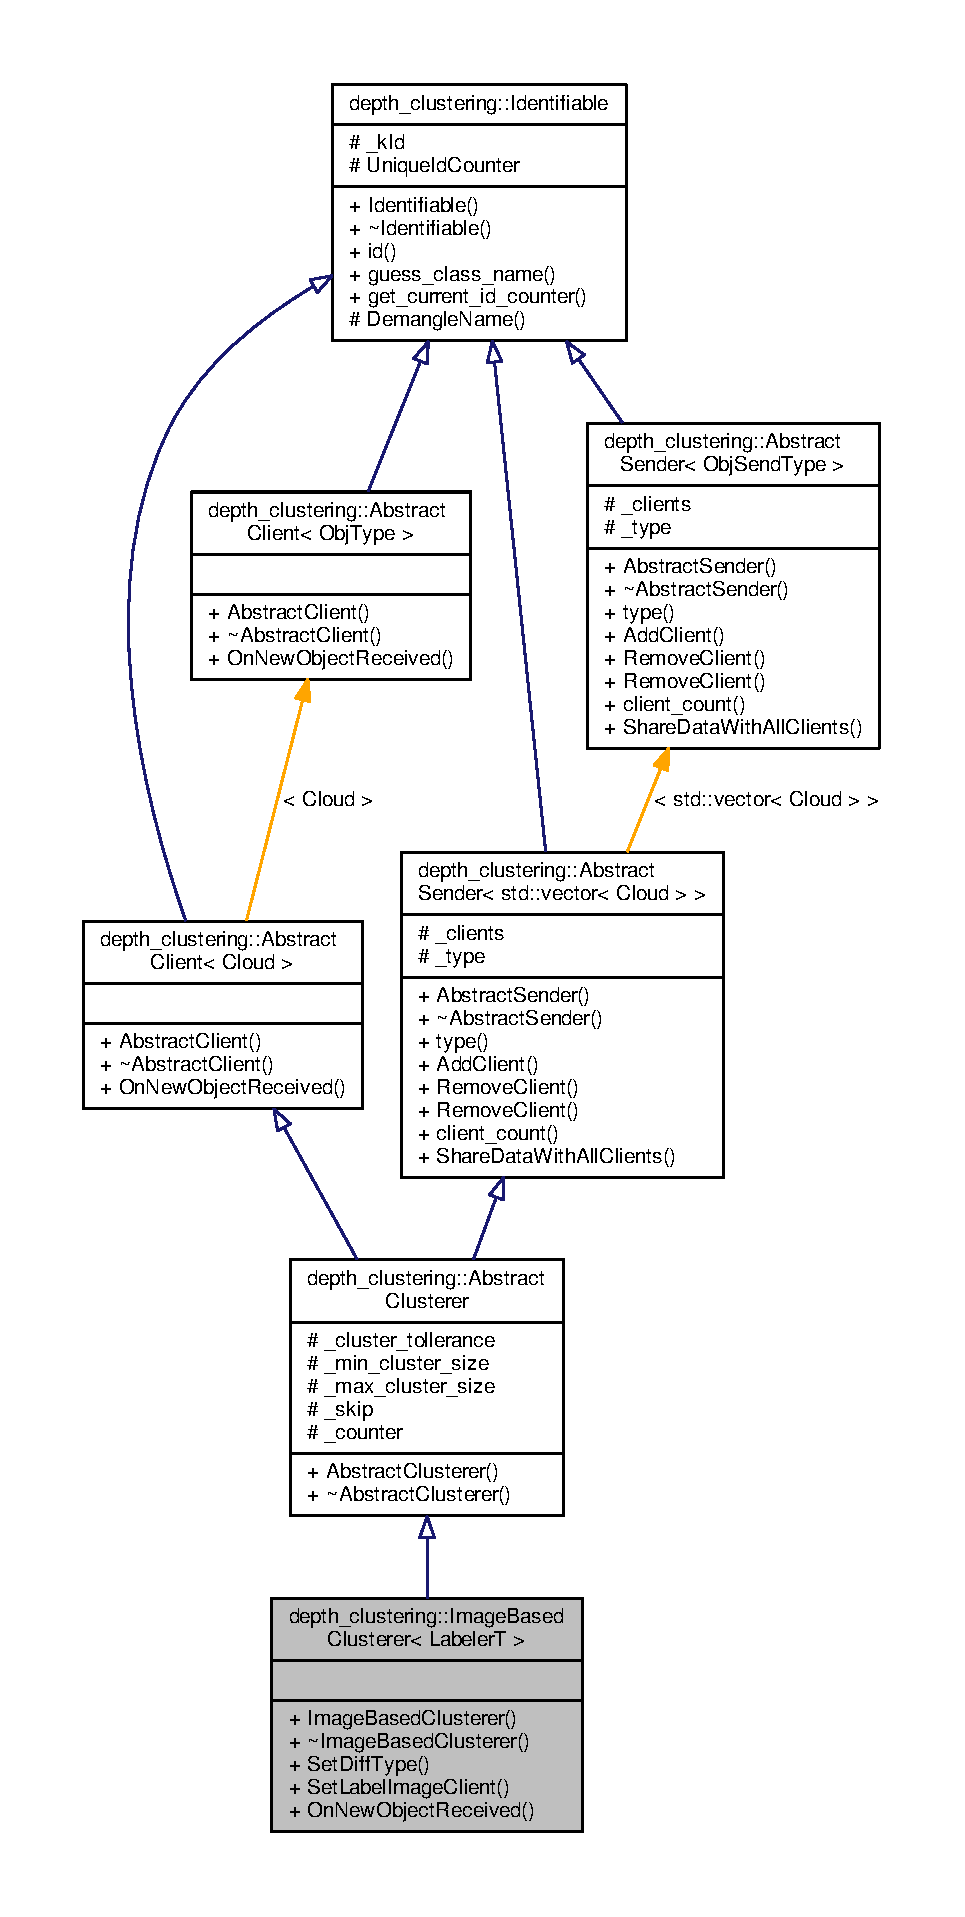
\includegraphics[height=550pt]{classdepth__clustering_1_1ImageBasedClusterer__inherit__graph}
\end{center}
\end{figure}


Collaboration diagram for depth\-\_\-clustering\-:\-:Image\-Based\-Clusterer$<$ Labeler\-T $>$\-:
\nopagebreak
\begin{figure}[H]
\begin{center}
\leavevmode
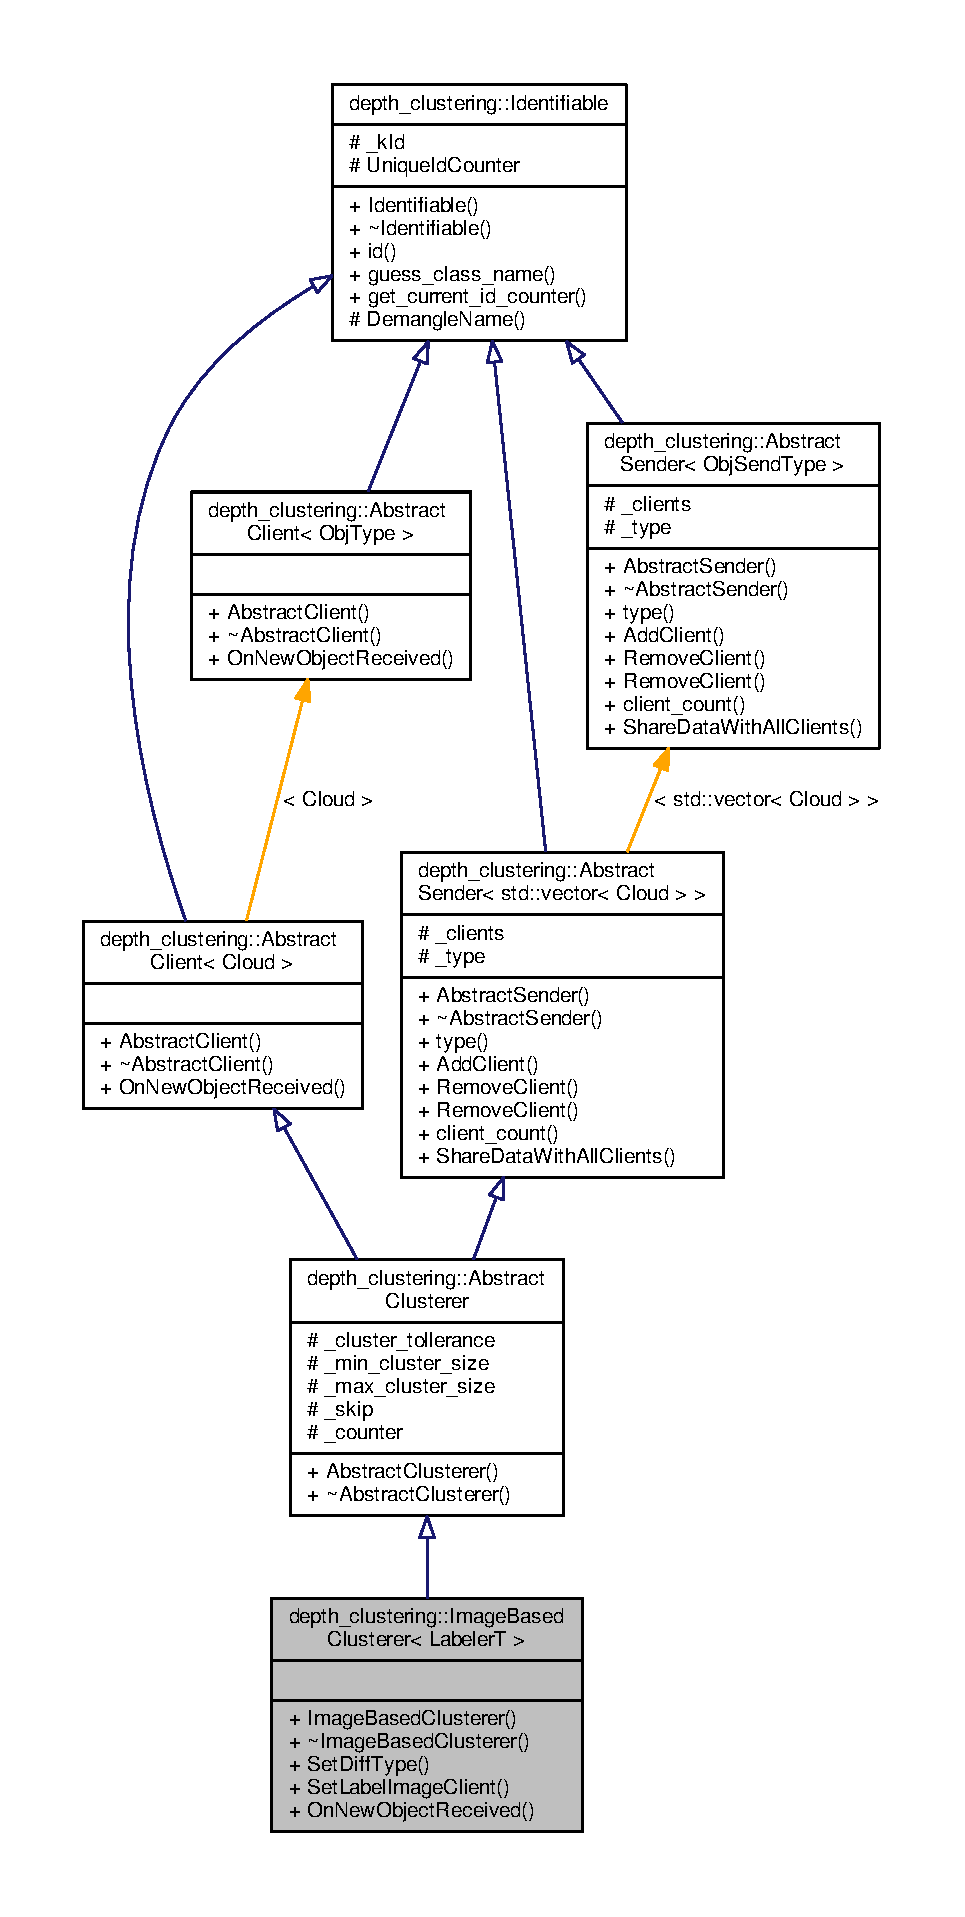
\includegraphics[height=550pt]{classdepth__clustering_1_1ImageBasedClusterer__coll__graph}
\end{center}
\end{figure}


\subsection{Constructor \& Destructor Documentation}
\hypertarget{classdepth__clustering_1_1ImageBasedClusterer_a6a8bdd77542e14ee420988ad80579f35}{\index{depth\-\_\-clustering\-::\-Image\-Based\-Clusterer@{depth\-\_\-clustering\-::\-Image\-Based\-Clusterer}!Image\-Based\-Clusterer@{Image\-Based\-Clusterer}}
\index{Image\-Based\-Clusterer@{Image\-Based\-Clusterer}!depth_clustering::ImageBasedClusterer@{depth\-\_\-clustering\-::\-Image\-Based\-Clusterer}}
\subsubsection[{Image\-Based\-Clusterer}]{\setlength{\rightskip}{0pt plus 5cm}template$<$typename Labeler\-T $>$ {\bf depth\-\_\-clustering\-::\-Image\-Based\-Clusterer}$<$ Labeler\-T $>$\-::{\bf Image\-Based\-Clusterer} (
\begin{DoxyParamCaption}
\item[{Radians}]{angle\-\_\-tollerance = {\ttfamily 8\-\_\-deg}, }
\item[{uint16\-\_\-t}]{min\-\_\-cluster\-\_\-size = {\ttfamily 100}, }
\item[{uint16\-\_\-t}]{max\-\_\-cluster\-\_\-size = {\ttfamily 25000}}
\end{DoxyParamCaption}
)\hspace{0.3cm}{\ttfamily [inline]}, {\ttfamily [explicit]}}}\label{classdepth__clustering_1_1ImageBasedClusterer_a6a8bdd77542e14ee420988ad80579f35}


Construct an image-\/based clusterer. 


\begin{DoxyParams}[1]{Parameters}
\mbox{\tt in}  & {\em angle\-\_\-tollerance} & The angle tollerance to separate objects \\
\hline
\mbox{\tt in}  & {\em min\-\_\-cluster\-\_\-size} & The minimum cluster size to send \\
\hline
\mbox{\tt in}  & {\em max\-\_\-cluster\-\_\-size} & The maximum cluster size to send \\
\hline
\end{DoxyParams}


\subsection{Member Function Documentation}
\hypertarget{classdepth__clustering_1_1ImageBasedClusterer_a825e11bfc35a0eeeac03341924ce3227}{\index{depth\-\_\-clustering\-::\-Image\-Based\-Clusterer@{depth\-\_\-clustering\-::\-Image\-Based\-Clusterer}!On\-New\-Object\-Received@{On\-New\-Object\-Received}}
\index{On\-New\-Object\-Received@{On\-New\-Object\-Received}!depth_clustering::ImageBasedClusterer@{depth\-\_\-clustering\-::\-Image\-Based\-Clusterer}}
\subsubsection[{On\-New\-Object\-Received}]{\setlength{\rightskip}{0pt plus 5cm}template$<$typename Labeler\-T $>$ void {\bf depth\-\_\-clustering\-::\-Image\-Based\-Clusterer}$<$ Labeler\-T $>$\-::On\-New\-Object\-Received (
\begin{DoxyParamCaption}
\item[{const {\bf Cloud} \&}]{cloud, }
\item[{const int}]{sender\-\_\-id}
\end{DoxyParamCaption}
)\hspace{0.3cm}{\ttfamily [inline]}, {\ttfamily [override]}, {\ttfamily [virtual]}}}\label{classdepth__clustering_1_1ImageBasedClusterer_a825e11bfc35a0eeeac03341924ce3227}


Gets called when clusterer receives a cloud to cluster. 


\begin{DoxyParams}[1]{Parameters}
\mbox{\tt in}  & {\em cloud} & The cloud to cluster \\
\hline
\mbox{\tt in}  & {\em sender\-\_\-id} & The sender identifier \\
\hline
\end{DoxyParams}


Implements \hyperlink{classdepth__clustering_1_1AbstractClient}{depth\-\_\-clustering\-::\-Abstract\-Client$<$ Cloud $>$}.



Here is the call graph for this function\-:
\nopagebreak
\begin{figure}[H]
\begin{center}
\leavevmode
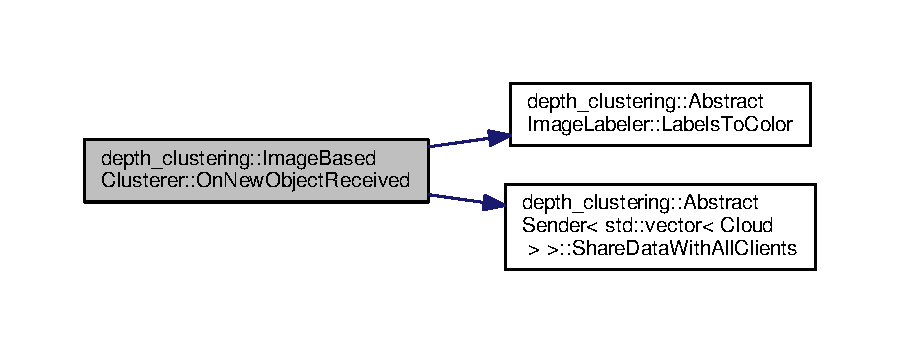
\includegraphics[width=350pt]{classdepth__clustering_1_1ImageBasedClusterer_a825e11bfc35a0eeeac03341924ce3227_cgraph}
\end{center}
\end{figure}


\hypertarget{classdepth__clustering_1_1ImageBasedClusterer_a0dd114829041816d309d6c8f9ff41cad}{\index{depth\-\_\-clustering\-::\-Image\-Based\-Clusterer@{depth\-\_\-clustering\-::\-Image\-Based\-Clusterer}!Set\-Diff\-Type@{Set\-Diff\-Type}}
\index{Set\-Diff\-Type@{Set\-Diff\-Type}!depth_clustering::ImageBasedClusterer@{depth\-\_\-clustering\-::\-Image\-Based\-Clusterer}}
\subsubsection[{Set\-Diff\-Type}]{\setlength{\rightskip}{0pt plus 5cm}template$<$typename Labeler\-T $>$ void {\bf depth\-\_\-clustering\-::\-Image\-Based\-Clusterer}$<$ Labeler\-T $>$\-::Set\-Diff\-Type (
\begin{DoxyParamCaption}
\item[{Diff\-Factory\-::\-Diff\-Type}]{diff\-\_\-type}
\end{DoxyParamCaption}
)\hspace{0.3cm}{\ttfamily [inline]}}}\label{classdepth__clustering_1_1ImageBasedClusterer_a0dd114829041816d309d6c8f9ff41cad}


Sets the difference type. 


\begin{DoxyParams}[1]{Parameters}
\mbox{\tt in}  & {\em diff\-\_\-type} & The difference type \\
\hline
\end{DoxyParams}
\hypertarget{classdepth__clustering_1_1ImageBasedClusterer_a6af0de0dad7450c34c655fb447886716}{\index{depth\-\_\-clustering\-::\-Image\-Based\-Clusterer@{depth\-\_\-clustering\-::\-Image\-Based\-Clusterer}!Set\-Label\-Image\-Client@{Set\-Label\-Image\-Client}}
\index{Set\-Label\-Image\-Client@{Set\-Label\-Image\-Client}!depth_clustering::ImageBasedClusterer@{depth\-\_\-clustering\-::\-Image\-Based\-Clusterer}}
\subsubsection[{Set\-Label\-Image\-Client}]{\setlength{\rightskip}{0pt plus 5cm}template$<$typename Labeler\-T $>$ void {\bf depth\-\_\-clustering\-::\-Image\-Based\-Clusterer}$<$ Labeler\-T $>$\-::Set\-Label\-Image\-Client (
\begin{DoxyParamCaption}
\item[{{\bf Abstract\-Client}$<$ cv\-::\-Mat $>$ $\ast$}]{client}
\end{DoxyParamCaption}
)\hspace{0.3cm}{\ttfamily [inline]}}}\label{classdepth__clustering_1_1ImageBasedClusterer_a6af0de0dad7450c34c655fb447886716}


Sets the label image client. 


\begin{DoxyParams}{Parameters}
{\em client} & The client to receive color images with labels \\
\hline
\end{DoxyParams}


The documentation for this class was generated from the following file\-:\begin{DoxyCompactItemize}
\item 
/home/hadoop/chy/depth\-\_\-clustering-\/master234/src/clusterers/image\-\_\-based\-\_\-clusterer.\-h\end{DoxyCompactItemize}

\hypertarget{classdepth__clustering_1_1LinearImageLabeler}{\section{depth\-\_\-clustering\-:\-:Linear\-Image\-Labeler$<$ S\-T\-E\-P\-\_\-\-R\-O\-W, S\-T\-E\-P\-\_\-\-C\-O\-L $>$ Class Template Reference}
\label{classdepth__clustering_1_1LinearImageLabeler}\index{depth\-\_\-clustering\-::\-Linear\-Image\-Labeler$<$ S\-T\-E\-P\-\_\-\-R\-O\-W, S\-T\-E\-P\-\_\-\-C\-O\-L $>$@{depth\-\_\-clustering\-::\-Linear\-Image\-Labeler$<$ S\-T\-E\-P\-\_\-\-R\-O\-W, S\-T\-E\-P\-\_\-\-C\-O\-L $>$}}
}


Class for linear image labeler.  




{\ttfamily \#include $<$linear\-\_\-image\-\_\-labeler.\-h$>$}

\subsection*{Public Member Functions}
\begin{DoxyCompactItemize}
\item 
\hyperlink{classdepth__clustering_1_1LinearImageLabeler_ad1026a0b49c300c6415691716b5acb99}{Linear\-Image\-Labeler} (const cv\-::\-Mat \&depth\-\_\-image, const \hyperlink{classdepth__clustering_1_1ProjectionParams}{Projection\-Params} \&params, const Radians \&angle\-\_\-threshold)
\begin{DoxyCompactList}\small\item\em Initialize Linear image labeler. \end{DoxyCompactList}\item 
void \hyperlink{classdepth__clustering_1_1LinearImageLabeler_ac5544f26628a05978a6a989ade6a1cd6}{Label\-One\-Component} (uint16\-\_\-t label, const \hyperlink{structdepth__clustering_1_1PixelCoord}{Pixel\-Coord} \&start, const \hyperlink{classdepth__clustering_1_1AbstractDiff}{Abstract\-Diff} $\ast$diff\-\_\-helper)
\begin{DoxyCompactList}\small\item\em Label a single connected component with B\-F\-S. Can be done faster if we augment the queue with a hash or smth. //如果我们采用\-B\-F\-S. \end{DoxyCompactList}\item 
float \hyperlink{classdepth__clustering_1_1LinearImageLabeler_a5fc990c42e9e017c7b5a949bf00010e5}{Depth\-At} (const \hyperlink{structdepth__clustering_1_1PixelCoord}{Pixel\-Coord} \&coord) const 
\begin{DoxyCompactList}\small\item\em Gets depth value at pixel. \end{DoxyCompactList}\item 
uint16\-\_\-t \hyperlink{classdepth__clustering_1_1LinearImageLabeler_a12c62dd4c7a8e58dad23e7c0d0efbade}{Label\-At} (const \hyperlink{structdepth__clustering_1_1PixelCoord}{Pixel\-Coord} \&coord) const 
\begin{DoxyCompactList}\small\item\em Gets label of a given pixel. \end{DoxyCompactList}\item 
void \hyperlink{classdepth__clustering_1_1LinearImageLabeler_a4693e920b2245f70206a11e141ddcb8f}{Set\-Label} (const \hyperlink{structdepth__clustering_1_1PixelCoord}{Pixel\-Coord} \&coord, uint16\-\_\-t label)
\begin{DoxyCompactList}\small\item\em Sets label of a given pixel. \end{DoxyCompactList}\item 
\hypertarget{classdepth__clustering_1_1LinearImageLabeler_a327b973bb85e30ce0a33c1e175d3bcb1}{int16\-\_\-t \hyperlink{classdepth__clustering_1_1LinearImageLabeler_a327b973bb85e30ce0a33c1e175d3bcb1}{Wrap\-Cols} (int16\-\_\-t col) const }\label{classdepth__clustering_1_1LinearImageLabeler_a327b973bb85e30ce0a33c1e175d3bcb1}

\begin{DoxyCompactList}\small\item\em Wrap columns around image. \end{DoxyCompactList}\item 
\hypertarget{classdepth__clustering_1_1LinearImageLabeler_a987cca7d9daab304af4bcc448bf6de0f}{void \hyperlink{classdepth__clustering_1_1LinearImageLabeler_a987cca7d9daab304af4bcc448bf6de0f}{Compute\-Labels} (Diff\-Factory\-::\-Diff\-Type diff\-\_\-type) override}\label{classdepth__clustering_1_1LinearImageLabeler_a987cca7d9daab304af4bcc448bf6de0f}

\begin{DoxyCompactList}\small\item\em Calculates the labels running over the whole image. \end{DoxyCompactList}\end{DoxyCompactItemize}
\subsection*{Public Attributes}
\begin{DoxyCompactItemize}
\item 
\hypertarget{classdepth__clustering_1_1LinearImageLabeler_a7237797a8c13b16aa3cdefe913d8c938}{std\-::array$<$ \hyperlink{structdepth__clustering_1_1PixelCoord}{Pixel\-Coord}, \\*
N\-E\-I\-G\-H\-\_\-\-S\-I\-Z\-E $>$ {\bfseries Neighborhood}}\label{classdepth__clustering_1_1LinearImageLabeler_a7237797a8c13b16aa3cdefe913d8c938}

\end{DoxyCompactItemize}
\subsection*{Static Public Attributes}
\begin{DoxyCompactItemize}
\item 
\hypertarget{classdepth__clustering_1_1LinearImageLabeler_ad6a78dde18091847582a7cea428ed5fb}{static constexpr int16\-\_\-t {\bfseries N\-E\-I\-G\-H\-\_\-\-S\-I\-Z\-E} = 2 $\ast$ S\-T\-E\-P\-\_\-\-R\-O\-W + 2 $\ast$ S\-T\-E\-P\-\_\-\-C\-O\-L}\label{classdepth__clustering_1_1LinearImageLabeler_ad6a78dde18091847582a7cea428ed5fb}

\end{DoxyCompactItemize}
\subsection*{Additional Inherited Members}


\subsection{Detailed Description}
\subsubsection*{template$<$int16\-\_\-t S\-T\-E\-P\-\_\-\-R\-O\-W = 1, int16\-\_\-t S\-T\-E\-P\-\_\-\-C\-O\-L = 1$>$class depth\-\_\-clustering\-::\-Linear\-Image\-Labeler$<$ S\-T\-E\-P\-\_\-\-R\-O\-W, S\-T\-E\-P\-\_\-\-C\-O\-L $>$}

Class for linear image labeler. 


\begin{DoxyTemplParams}{Template Parameters}
{\em S\-T\-E\-P\-\_\-\-R\-O\-W} & step we do over image over rows \\
\hline
{\em S\-T\-E\-P\-\_\-\-C\-O\-L} & step we do over image over cols \\
\hline
\end{DoxyTemplParams}


Inheritance diagram for depth\-\_\-clustering\-:\-:Linear\-Image\-Labeler$<$ S\-T\-E\-P\-\_\-\-R\-O\-W, S\-T\-E\-P\-\_\-\-C\-O\-L $>$\-:
\nopagebreak
\begin{figure}[H]
\begin{center}
\leavevmode
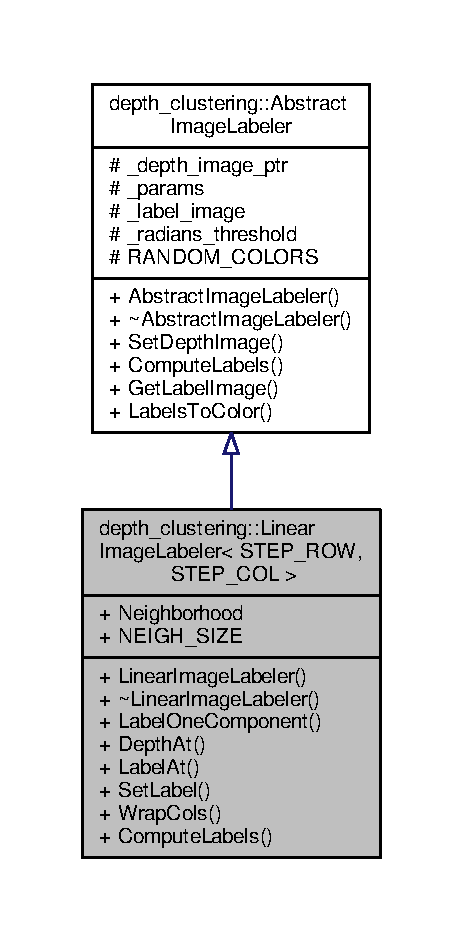
\includegraphics[width=222pt]{classdepth__clustering_1_1LinearImageLabeler__inherit__graph}
\end{center}
\end{figure}


Collaboration diagram for depth\-\_\-clustering\-:\-:Linear\-Image\-Labeler$<$ S\-T\-E\-P\-\_\-\-R\-O\-W, S\-T\-E\-P\-\_\-\-C\-O\-L $>$\-:
\nopagebreak
\begin{figure}[H]
\begin{center}
\leavevmode
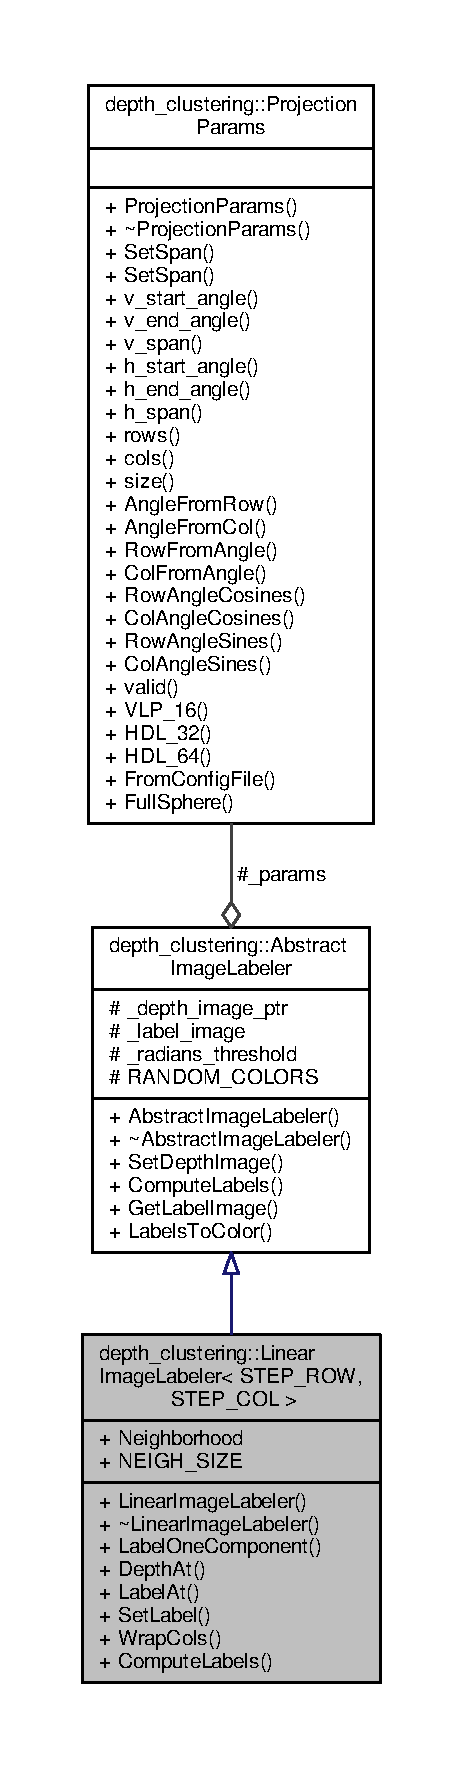
\includegraphics[height=550pt]{classdepth__clustering_1_1LinearImageLabeler__coll__graph}
\end{center}
\end{figure}


\subsection{Constructor \& Destructor Documentation}
\hypertarget{classdepth__clustering_1_1LinearImageLabeler_ad1026a0b49c300c6415691716b5acb99}{\index{depth\-\_\-clustering\-::\-Linear\-Image\-Labeler@{depth\-\_\-clustering\-::\-Linear\-Image\-Labeler}!Linear\-Image\-Labeler@{Linear\-Image\-Labeler}}
\index{Linear\-Image\-Labeler@{Linear\-Image\-Labeler}!depth_clustering::LinearImageLabeler@{depth\-\_\-clustering\-::\-Linear\-Image\-Labeler}}
\subsubsection[{Linear\-Image\-Labeler}]{\setlength{\rightskip}{0pt plus 5cm}template$<$int16\-\_\-t S\-T\-E\-P\-\_\-\-R\-O\-W = 1, int16\-\_\-t S\-T\-E\-P\-\_\-\-C\-O\-L = 1$>$ {\bf depth\-\_\-clustering\-::\-Linear\-Image\-Labeler}$<$ S\-T\-E\-P\-\_\-\-R\-O\-W, S\-T\-E\-P\-\_\-\-C\-O\-L $>$\-::{\bf Linear\-Image\-Labeler} (
\begin{DoxyParamCaption}
\item[{const cv\-::\-Mat \&}]{depth\-\_\-image, }
\item[{const {\bf Projection\-Params} \&}]{params, }
\item[{const Radians \&}]{angle\-\_\-threshold}
\end{DoxyParamCaption}
)\hspace{0.3cm}{\ttfamily [inline]}, {\ttfamily [explicit]}}}\label{classdepth__clustering_1_1LinearImageLabeler_ad1026a0b49c300c6415691716b5acb99}


Initialize Linear image labeler. 


\begin{DoxyParams}[1]{Parameters}
\mbox{\tt in}  & {\em depth\-\_\-image} & The depth image \\
\hline
\mbox{\tt in}  & {\em params} & The projection parameters \\
\hline
\mbox{\tt in}  & {\em angle\-\_\-threshold} & The angle threshold to seaparate clusters \\
\hline
\end{DoxyParams}


\subsection{Member Function Documentation}
\hypertarget{classdepth__clustering_1_1LinearImageLabeler_a5fc990c42e9e017c7b5a949bf00010e5}{\index{depth\-\_\-clustering\-::\-Linear\-Image\-Labeler@{depth\-\_\-clustering\-::\-Linear\-Image\-Labeler}!Depth\-At@{Depth\-At}}
\index{Depth\-At@{Depth\-At}!depth_clustering::LinearImageLabeler@{depth\-\_\-clustering\-::\-Linear\-Image\-Labeler}}
\subsubsection[{Depth\-At}]{\setlength{\rightskip}{0pt plus 5cm}template$<$int16\-\_\-t S\-T\-E\-P\-\_\-\-R\-O\-W = 1, int16\-\_\-t S\-T\-E\-P\-\_\-\-C\-O\-L = 1$>$ float {\bf depth\-\_\-clustering\-::\-Linear\-Image\-Labeler}$<$ S\-T\-E\-P\-\_\-\-R\-O\-W, S\-T\-E\-P\-\_\-\-C\-O\-L $>$\-::Depth\-At (
\begin{DoxyParamCaption}
\item[{const {\bf Pixel\-Coord} \&}]{coord}
\end{DoxyParamCaption}
) const\hspace{0.3cm}{\ttfamily [inline]}}}\label{classdepth__clustering_1_1LinearImageLabeler_a5fc990c42e9e017c7b5a949bf00010e5}


Gets depth value at pixel. 


\begin{DoxyParams}[1]{Parameters}
\mbox{\tt in}  & {\em coord} & Pixel coordinate//坐标像素坐标\\
\hline
\end{DoxyParams}
\begin{DoxyReturn}{Returns}
depth at pixel 
\end{DoxyReturn}


Here is the caller graph for this function\-:
\nopagebreak
\begin{figure}[H]
\begin{center}
\leavevmode
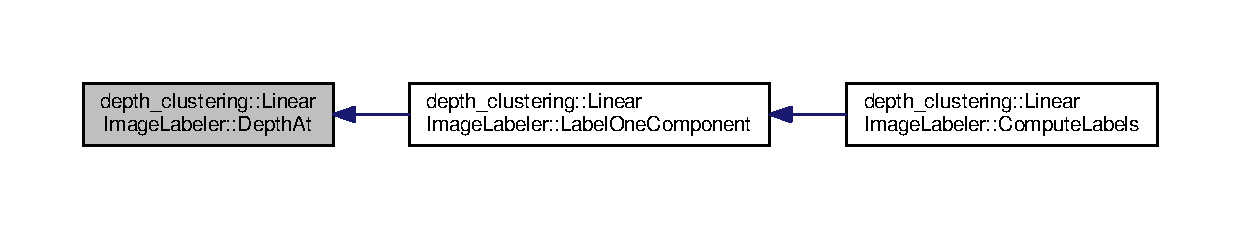
\includegraphics[width=350pt]{classdepth__clustering_1_1LinearImageLabeler_a5fc990c42e9e017c7b5a949bf00010e5_icgraph}
\end{center}
\end{figure}


\hypertarget{classdepth__clustering_1_1LinearImageLabeler_a12c62dd4c7a8e58dad23e7c0d0efbade}{\index{depth\-\_\-clustering\-::\-Linear\-Image\-Labeler@{depth\-\_\-clustering\-::\-Linear\-Image\-Labeler}!Label\-At@{Label\-At}}
\index{Label\-At@{Label\-At}!depth_clustering::LinearImageLabeler@{depth\-\_\-clustering\-::\-Linear\-Image\-Labeler}}
\subsubsection[{Label\-At}]{\setlength{\rightskip}{0pt plus 5cm}template$<$int16\-\_\-t S\-T\-E\-P\-\_\-\-R\-O\-W = 1, int16\-\_\-t S\-T\-E\-P\-\_\-\-C\-O\-L = 1$>$ uint16\-\_\-t {\bf depth\-\_\-clustering\-::\-Linear\-Image\-Labeler}$<$ S\-T\-E\-P\-\_\-\-R\-O\-W, S\-T\-E\-P\-\_\-\-C\-O\-L $>$\-::Label\-At (
\begin{DoxyParamCaption}
\item[{const {\bf Pixel\-Coord} \&}]{coord}
\end{DoxyParamCaption}
) const\hspace{0.3cm}{\ttfamily [inline]}}}\label{classdepth__clustering_1_1LinearImageLabeler_a12c62dd4c7a8e58dad23e7c0d0efbade}


Gets label of a given pixel. 


\begin{DoxyParams}[1]{Parameters}
\mbox{\tt in}  & {\em coord} & Pixel coordinate\\
\hline
\end{DoxyParams}
\begin{DoxyReturn}{Returns}
label for pixel 
\end{DoxyReturn}


Here is the caller graph for this function\-:
\nopagebreak
\begin{figure}[H]
\begin{center}
\leavevmode
\includegraphics[width=350pt]{classdepth__clustering_1_1LinearImageLabeler_a12c62dd4c7a8e58dad23e7c0d0efbade_icgraph}
\end{center}
\end{figure}


\hypertarget{classdepth__clustering_1_1LinearImageLabeler_ac5544f26628a05978a6a989ade6a1cd6}{\index{depth\-\_\-clustering\-::\-Linear\-Image\-Labeler@{depth\-\_\-clustering\-::\-Linear\-Image\-Labeler}!Label\-One\-Component@{Label\-One\-Component}}
\index{Label\-One\-Component@{Label\-One\-Component}!depth_clustering::LinearImageLabeler@{depth\-\_\-clustering\-::\-Linear\-Image\-Labeler}}
\subsubsection[{Label\-One\-Component}]{\setlength{\rightskip}{0pt plus 5cm}template$<$int16\-\_\-t S\-T\-E\-P\-\_\-\-R\-O\-W = 1, int16\-\_\-t S\-T\-E\-P\-\_\-\-C\-O\-L = 1$>$ void {\bf depth\-\_\-clustering\-::\-Linear\-Image\-Labeler}$<$ S\-T\-E\-P\-\_\-\-R\-O\-W, S\-T\-E\-P\-\_\-\-C\-O\-L $>$\-::Label\-One\-Component (
\begin{DoxyParamCaption}
\item[{uint16\-\_\-t}]{label, }
\item[{const {\bf Pixel\-Coord} \&}]{start, }
\item[{const {\bf Abstract\-Diff} $\ast$}]{diff\-\_\-helper}
\end{DoxyParamCaption}
)\hspace{0.3cm}{\ttfamily [inline]}}}\label{classdepth__clustering_1_1LinearImageLabeler_ac5544f26628a05978a6a989ade6a1cd6}


Label a single connected component with B\-F\-S. Can be done faster if we augment the queue with a hash or smth. //如果我们采用\-B\-F\-S. 


\begin{DoxyParams}[1]{Parameters}
\mbox{\tt in}  & {\em label} & Label this component with this label \\
\hline
\mbox{\tt in}  & {\em start} & Start pixel \\
\hline
\mbox{\tt in}  & {\em diff\-\_\-helper} & The difference helper Diff\-At \\
\hline
\end{DoxyParams}
std\-::cout$<$$<$\char`\"{}\-Now it runs in the Label\-One\-Component function  in the liner\-\_\-image\-\_\-lable .\-h\char`\"{}$<$$<$std\-::endl; 

Here is the call graph for this function\-:
\nopagebreak
\begin{figure}[H]
\begin{center}
\leavevmode
\includegraphics[width=350pt]{classdepth__clustering_1_1LinearImageLabeler_ac5544f26628a05978a6a989ade6a1cd6_cgraph}
\end{center}
\end{figure}




Here is the caller graph for this function\-:
\nopagebreak
\begin{figure}[H]
\begin{center}
\leavevmode
\includegraphics[width=350pt]{classdepth__clustering_1_1LinearImageLabeler_ac5544f26628a05978a6a989ade6a1cd6_icgraph}
\end{center}
\end{figure}


\hypertarget{classdepth__clustering_1_1LinearImageLabeler_a4693e920b2245f70206a11e141ddcb8f}{\index{depth\-\_\-clustering\-::\-Linear\-Image\-Labeler@{depth\-\_\-clustering\-::\-Linear\-Image\-Labeler}!Set\-Label@{Set\-Label}}
\index{Set\-Label@{Set\-Label}!depth_clustering::LinearImageLabeler@{depth\-\_\-clustering\-::\-Linear\-Image\-Labeler}}
\subsubsection[{Set\-Label}]{\setlength{\rightskip}{0pt plus 5cm}template$<$int16\-\_\-t S\-T\-E\-P\-\_\-\-R\-O\-W = 1, int16\-\_\-t S\-T\-E\-P\-\_\-\-C\-O\-L = 1$>$ void {\bf depth\-\_\-clustering\-::\-Linear\-Image\-Labeler}$<$ S\-T\-E\-P\-\_\-\-R\-O\-W, S\-T\-E\-P\-\_\-\-C\-O\-L $>$\-::Set\-Label (
\begin{DoxyParamCaption}
\item[{const {\bf Pixel\-Coord} \&}]{coord, }
\item[{uint16\-\_\-t}]{label}
\end{DoxyParamCaption}
)\hspace{0.3cm}{\ttfamily [inline]}}}\label{classdepth__clustering_1_1LinearImageLabeler_a4693e920b2245f70206a11e141ddcb8f}


Sets label of a given pixel. 


\begin{DoxyParams}[1]{Parameters}
\mbox{\tt in}  & {\em coord} & Pixel coordinate \\
\hline
\end{DoxyParams}


Here is the caller graph for this function\-:
\nopagebreak
\begin{figure}[H]
\begin{center}
\leavevmode
\includegraphics[width=350pt]{classdepth__clustering_1_1LinearImageLabeler_a4693e920b2245f70206a11e141ddcb8f_icgraph}
\end{center}
\end{figure}




The documentation for this class was generated from the following file\-:\begin{DoxyCompactItemize}
\item 
/home/hadoop/chy/depth\-\_\-clustering-\/master234/src/image\-\_\-labelers/linear\-\_\-image\-\_\-labeler.\-h\end{DoxyCompactItemize}

\hypertarget{classdepth__clustering_1_1LineDistDiff}{\section{depth\-\_\-clustering\-:\-:Line\-Dist\-Diff Class Reference}
\label{classdepth__clustering_1_1LineDistDiff}\index{depth\-\_\-clustering\-::\-Line\-Dist\-Diff@{depth\-\_\-clustering\-::\-Line\-Dist\-Diff}}
}


Class for line-\/based difference. It is very alike to \hyperlink{classdepth__clustering_1_1AngleDiff}{Angle\-Diff} class, just that after we have computed the angle, we compute $d_1 sin(\beta)$ to get the distance to the line spawned with two measurements.  




{\ttfamily \#include $<$line\-\_\-dist\-\_\-diff.\-h$>$}

\subsection*{Public Member Functions}
\begin{DoxyCompactItemize}
\item 
\hyperlink{classdepth__clustering_1_1LineDistDiff_af922d3e19bc52a2fdbf36317fc474d88}{Line\-Dist\-Diff} (const cv\-::\-Mat $\ast$source\-\_\-image, const \hyperlink{classdepth__clustering_1_1ProjectionParams}{Projection\-Params} $\ast$params)
\begin{DoxyCompactList}\small\item\em Precompute the line distances to avoid losing time on that. \end{DoxyCompactList}\item 
float \hyperlink{classdepth__clustering_1_1LineDistDiff_a839eee44b14de26d85e6dbad5e37b356}{Diff\-At} (const \hyperlink{structdepth__clustering_1_1PixelCoord}{Pixel\-Coord} \&from, const \hyperlink{structdepth__clustering_1_1PixelCoord}{Pixel\-Coord} \&to) const override
\begin{DoxyCompactList}\small\item\em Compute angle-\/based difference. See paper for details. \end{DoxyCompactList}\item 
\hypertarget{classdepth__clustering_1_1LineDistDiff_ae9debede2cffd6bb40ca4c4a82c52f61}{bool \hyperlink{classdepth__clustering_1_1LineDistDiff_ae9debede2cffd6bb40ca4c4a82c52f61}{Satisfies\-Threshold} (float angle, float threshold) const override}\label{classdepth__clustering_1_1LineDistDiff_ae9debede2cffd6bb40ca4c4a82c52f61}

\begin{DoxyCompactList}\small\item\em Threshold is satisfied if angle is B\-I\-G\-G\-E\-R than threshold. \end{DoxyCompactList}\item 
cv\-::\-Mat \hyperlink{classdepth__clustering_1_1LineDistDiff_a7feaf820589ccfb47786d5124a74d725}{Visualize} () const override
\begin{DoxyCompactList}\small\item\em Visualize $\beta$ angles as a {\ttfamily cv\-::\-Mat} color image. \end{DoxyCompactList}\end{DoxyCompactItemize}
\subsection*{Additional Inherited Members}


\subsection{Detailed Description}
Class for line-\/based difference. It is very alike to \hyperlink{classdepth__clustering_1_1AngleDiff}{Angle\-Diff} class, just that after we have computed the angle, we compute $d_1 sin(\beta)$ to get the distance to the line spawned with two measurements. 

Inheritance diagram for depth\-\_\-clustering\-:\-:Line\-Dist\-Diff\-:
\nopagebreak
\begin{figure}[H]
\begin{center}
\leavevmode
\includegraphics[width=226pt]{classdepth__clustering_1_1LineDistDiff__inherit__graph}
\end{center}
\end{figure}


Collaboration diagram for depth\-\_\-clustering\-:\-:Line\-Dist\-Diff\-:
\nopagebreak
\begin{figure}[H]
\begin{center}
\leavevmode
\includegraphics[width=226pt]{classdepth__clustering_1_1LineDistDiff__coll__graph}
\end{center}
\end{figure}


\subsection{Constructor \& Destructor Documentation}
\hypertarget{classdepth__clustering_1_1LineDistDiff_af922d3e19bc52a2fdbf36317fc474d88}{\index{depth\-\_\-clustering\-::\-Line\-Dist\-Diff@{depth\-\_\-clustering\-::\-Line\-Dist\-Diff}!Line\-Dist\-Diff@{Line\-Dist\-Diff}}
\index{Line\-Dist\-Diff@{Line\-Dist\-Diff}!depth_clustering::LineDistDiff@{depth\-\_\-clustering\-::\-Line\-Dist\-Diff}}
\subsubsection[{Line\-Dist\-Diff}]{\setlength{\rightskip}{0pt plus 5cm}depth\-\_\-clustering\-::\-Line\-Dist\-Diff\-::\-Line\-Dist\-Diff (
\begin{DoxyParamCaption}
\item[{const cv\-::\-Mat $\ast$}]{source\-\_\-image, }
\item[{const {\bf Projection\-Params} $\ast$}]{params}
\end{DoxyParamCaption}
)}}\label{classdepth__clustering_1_1LineDistDiff_af922d3e19bc52a2fdbf36317fc474d88}


Precompute the line distances to avoid losing time on that. 


\begin{DoxyParams}[1]{Parameters}
\mbox{\tt in}  & {\em source\-\_\-image} & The source image \\
\hline
\mbox{\tt in}  & {\em params} & The projection parameters \\
\hline
\end{DoxyParams}


\subsection{Member Function Documentation}
\hypertarget{classdepth__clustering_1_1LineDistDiff_a839eee44b14de26d85e6dbad5e37b356}{\index{depth\-\_\-clustering\-::\-Line\-Dist\-Diff@{depth\-\_\-clustering\-::\-Line\-Dist\-Diff}!Diff\-At@{Diff\-At}}
\index{Diff\-At@{Diff\-At}!depth_clustering::LineDistDiff@{depth\-\_\-clustering\-::\-Line\-Dist\-Diff}}
\subsubsection[{Diff\-At}]{\setlength{\rightskip}{0pt plus 5cm}float depth\-\_\-clustering\-::\-Line\-Dist\-Diff\-::\-Diff\-At (
\begin{DoxyParamCaption}
\item[{const {\bf Pixel\-Coord} \&}]{from, }
\item[{const {\bf Pixel\-Coord} \&}]{to}
\end{DoxyParamCaption}
) const\hspace{0.3cm}{\ttfamily [override]}, {\ttfamily [virtual]}}}\label{classdepth__clustering_1_1LineDistDiff_a839eee44b14de26d85e6dbad5e37b356}


Compute angle-\/based difference. See paper for details. 


\begin{DoxyParams}[1]{Parameters}
\mbox{\tt in}  & {\em from} & Pixel from which to compute difference \\
\hline
\mbox{\tt in}  & {\em to} & Pixel to which to compute difference\\
\hline
\end{DoxyParams}
\begin{DoxyReturn}{Returns}
Angle difference between the values 
\end{DoxyReturn}


Implements \hyperlink{classdepth__clustering_1_1AbstractDiff_a06ba188d8d83d0e4bad66c833656c26d}{depth\-\_\-clustering\-::\-Abstract\-Diff}.

\hypertarget{classdepth__clustering_1_1LineDistDiff_a7feaf820589ccfb47786d5124a74d725}{\index{depth\-\_\-clustering\-::\-Line\-Dist\-Diff@{depth\-\_\-clustering\-::\-Line\-Dist\-Diff}!Visualize@{Visualize}}
\index{Visualize@{Visualize}!depth_clustering::LineDistDiff@{depth\-\_\-clustering\-::\-Line\-Dist\-Diff}}
\subsubsection[{Visualize}]{\setlength{\rightskip}{0pt plus 5cm}cv\-::\-Mat depth\-\_\-clustering\-::\-Line\-Dist\-Diff\-::\-Visualize (
\begin{DoxyParamCaption}
{}
\end{DoxyParamCaption}
) const\hspace{0.3cm}{\ttfamily [inline]}, {\ttfamily [override]}, {\ttfamily [virtual]}}}\label{classdepth__clustering_1_1LineDistDiff_a7feaf820589ccfb47786d5124a74d725}


Visualize $\beta$ angles as a {\ttfamily cv\-::\-Mat} color image. 

\begin{DoxyReturn}{Returns}
{\ttfamily cv\-::\-Mat} color image with red channel showing $\beta$ angles in row direction and green channel in col direction. 
\end{DoxyReturn}


Reimplemented from \hyperlink{classdepth__clustering_1_1AbstractDiff_a5500c82f3e6800922ba6fc6c22c6d0bf}{depth\-\_\-clustering\-::\-Abstract\-Diff}.



The documentation for this class was generated from the following files\-:\begin{DoxyCompactItemize}
\item 
/home/hadoop/chy/depth\-\_\-clustering-\/master234/src/image\-\_\-labelers/diff\-\_\-helpers/line\-\_\-dist\-\_\-diff.\-h\item 
/home/hadoop/chy/depth\-\_\-clustering-\/master234/src/image\-\_\-labelers/diff\-\_\-helpers/line\-\_\-dist\-\_\-diff.\-cpp\end{DoxyCompactItemize}

\hypertarget{classdepth__clustering_1_1LineDistDiffPrecomputed}{\section{depth\-\_\-clustering\-:\-:Line\-Dist\-Diff\-Precomputed Class Reference}
\label{classdepth__clustering_1_1LineDistDiffPrecomputed}\index{depth\-\_\-clustering\-::\-Line\-Dist\-Diff\-Precomputed@{depth\-\_\-clustering\-::\-Line\-Dist\-Diff\-Precomputed}}
}


Class for angle difference.  




{\ttfamily \#include $<$line\-\_\-dist\-\_\-diff.\-h$>$}

\subsection*{Public Member Functions}
\begin{DoxyCompactItemize}
\item 
\hyperlink{classdepth__clustering_1_1LineDistDiffPrecomputed_a035909e1718ad9b54b9b4116bbb6c408}{Line\-Dist\-Diff\-Precomputed} (const cv\-::\-Mat $\ast$source\-\_\-image, const \hyperlink{classdepth__clustering_1_1ProjectionParams}{Projection\-Params} $\ast$params)
\begin{DoxyCompactList}\small\item\em Precompute the angles to avoid losing time on that. \end{DoxyCompactList}\item 
float \hyperlink{classdepth__clustering_1_1LineDistDiffPrecomputed_ac505afaa537656af1bcc342ab1e910c4}{Diff\-At} (const \hyperlink{structdepth__clustering_1_1PixelCoord}{Pixel\-Coord} \&from, const \hyperlink{structdepth__clustering_1_1PixelCoord}{Pixel\-Coord} \&to) const override
\begin{DoxyCompactList}\small\item\em Compute angle-\/based difference. See paper for details. Only one of the following situations is possible\-: \end{DoxyCompactList}\item 
\hypertarget{classdepth__clustering_1_1LineDistDiffPrecomputed_ac3ce8196d5e6f49f3e3bdc3e3b32b033}{bool \hyperlink{classdepth__clustering_1_1LineDistDiffPrecomputed_ac3ce8196d5e6f49f3e3bdc3e3b32b033}{Satisfies\-Threshold} (float angle, float threshold) const override}\label{classdepth__clustering_1_1LineDistDiffPrecomputed_ac3ce8196d5e6f49f3e3bdc3e3b32b033}

\begin{DoxyCompactList}\small\item\em Threshold is satisfied if angle is B\-I\-G\-G\-E\-R than threshold. \end{DoxyCompactList}\item 
cv\-::\-Mat \hyperlink{classdepth__clustering_1_1LineDistDiffPrecomputed_ae06f8b4dd6330730849725c1b1f20b43}{Visualize} () const 
\begin{DoxyCompactList}\small\item\em Visualize $\beta$ angles as a {\ttfamily cv\-::\-Mat} color image. \end{DoxyCompactList}\end{DoxyCompactItemize}
\subsection*{Protected Member Functions}
\begin{DoxyCompactItemize}
\item 
\hypertarget{classdepth__clustering_1_1LineDistDiffPrecomputed_a9e52e2a94d9f92567953a765475d62a0}{void \hyperlink{classdepth__clustering_1_1LineDistDiffPrecomputed_a9e52e2a94d9f92567953a765475d62a0}{Pre\-Compute\-Alpha\-Vecs} ()}\label{classdepth__clustering_1_1LineDistDiffPrecomputed_a9e52e2a94d9f92567953a765475d62a0}

\begin{DoxyCompactList}\small\item\em Pre-\/compute values for angles for all cols and rows. \end{DoxyCompactList}\item 
void \hyperlink{classdepth__clustering_1_1LineDistDiffPrecomputed_a9d0211af30be1f60ef4e8db570128a7b}{Pre\-Compute\-Line\-Dists} ()
\begin{DoxyCompactList}\small\item\em Precompute all $\beta$ angles for the image. It generates two matrices for row-\/wise and col-\/wise angles. See picture for illustration. The squares store values of angles between pixels with computation direction shown by arrows. Note that the columns matrix wraps around, i.\-e. the last element stores the difference in angles between the last pixel of the original image and the first one. \end{DoxyCompactList}\item 
float \hyperlink{classdepth__clustering_1_1LineDistDiffPrecomputed_a77df0f089f743ee9b586a7eb369c0257}{Get\-Line\-Dist} (float alpha, float current\-\_\-depth, float neighbor\-\_\-depth) const 
\begin{DoxyCompactList}\small\item\em Compute the angle $\beta$ of incline of the line spawned by two given beams. \end{DoxyCompactList}\end{DoxyCompactItemize}
\subsection*{Protected Attributes}
\begin{DoxyCompactItemize}
\item 
\hypertarget{classdepth__clustering_1_1LineDistDiffPrecomputed_aeb0f0894cc1f1fcbd9d40813005432f3}{const \hyperlink{classdepth__clustering_1_1ProjectionParams}{Projection\-Params} $\ast$ {\bfseries \-\_\-params} = nullptr}\label{classdepth__clustering_1_1LineDistDiffPrecomputed_aeb0f0894cc1f1fcbd9d40813005432f3}

\item 
\hypertarget{classdepth__clustering_1_1LineDistDiffPrecomputed_a5694d6392f56f8659f048f6df7f0ba93}{std\-::vector$<$ float $>$ {\bfseries \-\_\-row\-\_\-alphas}}\label{classdepth__clustering_1_1LineDistDiffPrecomputed_a5694d6392f56f8659f048f6df7f0ba93}

\item 
\hypertarget{classdepth__clustering_1_1LineDistDiffPrecomputed_a0c9b6dc3de39f95b8a76061e94e85505}{std\-::vector$<$ float $>$ {\bfseries \-\_\-col\-\_\-alphas}}\label{classdepth__clustering_1_1LineDistDiffPrecomputed_a0c9b6dc3de39f95b8a76061e94e85505}

\item 
\hypertarget{classdepth__clustering_1_1LineDistDiffPrecomputed_aa4f24cff932c5d498c01ec71179a5e89}{cv\-::\-Mat {\bfseries \-\_\-dists\-\_\-row}}\label{classdepth__clustering_1_1LineDistDiffPrecomputed_aa4f24cff932c5d498c01ec71179a5e89}

\item 
\hypertarget{classdepth__clustering_1_1LineDistDiffPrecomputed_ac0a7cd72ad073091beaefa1d6b3da4a1}{cv\-::\-Mat {\bfseries \-\_\-dists\-\_\-col}}\label{classdepth__clustering_1_1LineDistDiffPrecomputed_ac0a7cd72ad073091beaefa1d6b3da4a1}

\end{DoxyCompactItemize}


\subsection{Detailed Description}
Class for angle difference. 

Inheritance diagram for depth\-\_\-clustering\-:\-:Line\-Dist\-Diff\-Precomputed\-:
\nopagebreak
\begin{figure}[H]
\begin{center}
\leavevmode
\includegraphics[width=226pt]{classdepth__clustering_1_1LineDistDiffPrecomputed__inherit__graph}
\end{center}
\end{figure}


Collaboration diagram for depth\-\_\-clustering\-:\-:Line\-Dist\-Diff\-Precomputed\-:
\nopagebreak
\begin{figure}[H]
\begin{center}
\leavevmode
\includegraphics[height=550pt]{classdepth__clustering_1_1LineDistDiffPrecomputed__coll__graph}
\end{center}
\end{figure}


\subsection{Constructor \& Destructor Documentation}
\hypertarget{classdepth__clustering_1_1LineDistDiffPrecomputed_a035909e1718ad9b54b9b4116bbb6c408}{\index{depth\-\_\-clustering\-::\-Line\-Dist\-Diff\-Precomputed@{depth\-\_\-clustering\-::\-Line\-Dist\-Diff\-Precomputed}!Line\-Dist\-Diff\-Precomputed@{Line\-Dist\-Diff\-Precomputed}}
\index{Line\-Dist\-Diff\-Precomputed@{Line\-Dist\-Diff\-Precomputed}!depth_clustering::LineDistDiffPrecomputed@{depth\-\_\-clustering\-::\-Line\-Dist\-Diff\-Precomputed}}
\subsubsection[{Line\-Dist\-Diff\-Precomputed}]{\setlength{\rightskip}{0pt plus 5cm}depth\-\_\-clustering\-::\-Line\-Dist\-Diff\-Precomputed\-::\-Line\-Dist\-Diff\-Precomputed (
\begin{DoxyParamCaption}
\item[{const cv\-::\-Mat $\ast$}]{source\-\_\-image, }
\item[{const {\bf Projection\-Params} $\ast$}]{params}
\end{DoxyParamCaption}
)}}\label{classdepth__clustering_1_1LineDistDiffPrecomputed_a035909e1718ad9b54b9b4116bbb6c408}


Precompute the angles to avoid losing time on that. 


\begin{DoxyParams}[1]{Parameters}
\mbox{\tt in}  & {\em source\-\_\-image} & The source image \\
\hline
\mbox{\tt in}  & {\em params} & The projection parameters \\
\hline
\end{DoxyParams}


\subsection{Member Function Documentation}
\hypertarget{classdepth__clustering_1_1LineDistDiffPrecomputed_ac505afaa537656af1bcc342ab1e910c4}{\index{depth\-\_\-clustering\-::\-Line\-Dist\-Diff\-Precomputed@{depth\-\_\-clustering\-::\-Line\-Dist\-Diff\-Precomputed}!Diff\-At@{Diff\-At}}
\index{Diff\-At@{Diff\-At}!depth_clustering::LineDistDiffPrecomputed@{depth\-\_\-clustering\-::\-Line\-Dist\-Diff\-Precomputed}}
\subsubsection[{Diff\-At}]{\setlength{\rightskip}{0pt plus 5cm}float depth\-\_\-clustering\-::\-Line\-Dist\-Diff\-Precomputed\-::\-Diff\-At (
\begin{DoxyParamCaption}
\item[{const {\bf Pixel\-Coord} \&}]{from, }
\item[{const {\bf Pixel\-Coord} \&}]{to}
\end{DoxyParamCaption}
) const\hspace{0.3cm}{\ttfamily [override]}, {\ttfamily [virtual]}}}\label{classdepth__clustering_1_1LineDistDiffPrecomputed_ac505afaa537656af1bcc342ab1e910c4}


Compute angle-\/based difference. See paper for details. Only one of the following situations is possible\-: 


\begin{DoxyItemize}
\item from.\-row $>$ to.\-row
\item from.\-row $<$ to.\-row
\item from.\-col $>$ to.\-col
\item from.\-col $<$ to.\-col
\end{DoxyItemize}


\begin{DoxyParams}[1]{Parameters}
\mbox{\tt in}  & {\em from} & Pixel from which to compute difference \\
\hline
\mbox{\tt in}  & {\em to} & Pixel to which to compute difference\\
\hline
\end{DoxyParams}
\begin{DoxyReturn}{Returns}
Angle difference between the values 
\end{DoxyReturn}
If one of rows is biggest possible -\/ use it. Otherwise use {\ttfamily std\-::min(from.\-row, to.\-row)}.

If one of cols is biggest possible -\/ use it. Otherwise use {\ttfamily std\-::min(from.\-col, to.\-col)}. 

Implements \hyperlink{classdepth__clustering_1_1AbstractDiff_a06ba188d8d83d0e4bad66c833656c26d}{depth\-\_\-clustering\-::\-Abstract\-Diff}.

\hypertarget{classdepth__clustering_1_1LineDistDiffPrecomputed_a77df0f089f743ee9b586a7eb369c0257}{\index{depth\-\_\-clustering\-::\-Line\-Dist\-Diff\-Precomputed@{depth\-\_\-clustering\-::\-Line\-Dist\-Diff\-Precomputed}!Get\-Line\-Dist@{Get\-Line\-Dist}}
\index{Get\-Line\-Dist@{Get\-Line\-Dist}!depth_clustering::LineDistDiffPrecomputed@{depth\-\_\-clustering\-::\-Line\-Dist\-Diff\-Precomputed}}
\subsubsection[{Get\-Line\-Dist}]{\setlength{\rightskip}{0pt plus 5cm}float depth\-\_\-clustering\-::\-Line\-Dist\-Diff\-Precomputed\-::\-Get\-Line\-Dist (
\begin{DoxyParamCaption}
\item[{float}]{alpha, }
\item[{float}]{current\-\_\-depth, }
\item[{float}]{neighbor\-\_\-depth}
\end{DoxyParamCaption}
) const\hspace{0.3cm}{\ttfamily [protected]}}}\label{classdepth__clustering_1_1LineDistDiffPrecomputed_a77df0f089f743ee9b586a7eb369c0257}


Compute the angle $\beta$ of incline of the line spawned by two given beams. 


\begin{DoxyParams}[1]{Parameters}
\mbox{\tt in}  & {\em alpha} & The angle $\alpha$ between the beams. \\
\hline
\mbox{\tt in}  & {\em current\-\_\-depth} & The reading of the first beam in meters. \\
\hline
\mbox{\tt in}  & {\em neighbor\-\_\-depth} & The reading of the second beam in meters.\\
\hline
\end{DoxyParams}
\begin{DoxyReturn}{Returns}
The angle of incidence of the line spawned by endpoints of two given beams. 
\end{DoxyReturn}


Here is the caller graph for this function\-:
\nopagebreak
\begin{figure}[H]
\begin{center}
\leavevmode
\includegraphics[width=350pt]{classdepth__clustering_1_1LineDistDiffPrecomputed_a77df0f089f743ee9b586a7eb369c0257_icgraph}
\end{center}
\end{figure}


\hypertarget{classdepth__clustering_1_1LineDistDiffPrecomputed_a9d0211af30be1f60ef4e8db570128a7b}{\index{depth\-\_\-clustering\-::\-Line\-Dist\-Diff\-Precomputed@{depth\-\_\-clustering\-::\-Line\-Dist\-Diff\-Precomputed}!Pre\-Compute\-Line\-Dists@{Pre\-Compute\-Line\-Dists}}
\index{Pre\-Compute\-Line\-Dists@{Pre\-Compute\-Line\-Dists}!depth_clustering::LineDistDiffPrecomputed@{depth\-\_\-clustering\-::\-Line\-Dist\-Diff\-Precomputed}}
\subsubsection[{Pre\-Compute\-Line\-Dists}]{\setlength{\rightskip}{0pt plus 5cm}void depth\-\_\-clustering\-::\-Line\-Dist\-Diff\-Precomputed\-::\-Pre\-Compute\-Line\-Dists (
\begin{DoxyParamCaption}
{}
\end{DoxyParamCaption}
)\hspace{0.3cm}{\ttfamily [protected]}}}\label{classdepth__clustering_1_1LineDistDiffPrecomputed_a9d0211af30be1f60ef4e8db570128a7b}


Precompute all $\beta$ angles for the image. It generates two matrices for row-\/wise and col-\/wise angles. See picture for illustration. The squares store values of angles between pixels with computation direction shown by arrows. Note that the columns matrix wraps around, i.\-e. the last element stores the difference in angles between the last pixel of the original image and the first one. 

 

Here is the call graph for this function\-:
\nopagebreak
\begin{figure}[H]
\begin{center}
\leavevmode
\includegraphics[width=350pt]{classdepth__clustering_1_1LineDistDiffPrecomputed_a9d0211af30be1f60ef4e8db570128a7b_cgraph}
\end{center}
\end{figure}


\hypertarget{classdepth__clustering_1_1LineDistDiffPrecomputed_ae06f8b4dd6330730849725c1b1f20b43}{\index{depth\-\_\-clustering\-::\-Line\-Dist\-Diff\-Precomputed@{depth\-\_\-clustering\-::\-Line\-Dist\-Diff\-Precomputed}!Visualize@{Visualize}}
\index{Visualize@{Visualize}!depth_clustering::LineDistDiffPrecomputed@{depth\-\_\-clustering\-::\-Line\-Dist\-Diff\-Precomputed}}
\subsubsection[{Visualize}]{\setlength{\rightskip}{0pt plus 5cm}cv\-::\-Mat depth\-\_\-clustering\-::\-Line\-Dist\-Diff\-Precomputed\-::\-Visualize (
\begin{DoxyParamCaption}
{}
\end{DoxyParamCaption}
) const\hspace{0.3cm}{\ttfamily [virtual]}}}\label{classdepth__clustering_1_1LineDistDiffPrecomputed_ae06f8b4dd6330730849725c1b1f20b43}


Visualize $\beta$ angles as a {\ttfamily cv\-::\-Mat} color image. 

\begin{DoxyReturn}{Returns}
{\ttfamily cv\-::\-Mat} color image with red channel showing $\beta$ angles in row direction and green channel in col direction. 
\end{DoxyReturn}


Reimplemented from \hyperlink{classdepth__clustering_1_1AbstractDiff_a5500c82f3e6800922ba6fc6c22c6d0bf}{depth\-\_\-clustering\-::\-Abstract\-Diff}.



The documentation for this class was generated from the following files\-:\begin{DoxyCompactItemize}
\item 
/home/hadoop/chy/depth\-\_\-clustering-\/master234/src/image\-\_\-labelers/diff\-\_\-helpers/line\-\_\-dist\-\_\-diff.\-h\item 
/home/hadoop/chy/depth\-\_\-clustering-\/master234/src/image\-\_\-labelers/diff\-\_\-helpers/line\-\_\-dist\-\_\-diff.\-cpp\end{DoxyCompactItemize}

\hypertarget{structdepth__clustering_1_1PixelCoord}{\section{depth\-\_\-clustering\-:\-:Pixel\-Coord Struct Reference}
\label{structdepth__clustering_1_1PixelCoord}\index{depth\-\_\-clustering\-::\-Pixel\-Coord@{depth\-\_\-clustering\-::\-Pixel\-Coord}}
}


Pixel coordinates structure.  




{\ttfamily \#include $<$pixel\-\_\-coords.\-h$>$}

\subsection*{Public Member Functions}
\begin{DoxyCompactItemize}
\item 
\hypertarget{structdepth__clustering_1_1PixelCoord_aff0f4516ef80598fce8f8fc7a2206ac4}{{\bfseries Pixel\-Coord} (int16\-\_\-t row\-\_\-, int16\-\_\-t col\-\_\-)}\label{structdepth__clustering_1_1PixelCoord_aff0f4516ef80598fce8f8fc7a2206ac4}

\item 
\hypertarget{structdepth__clustering_1_1PixelCoord_af661ad9672b6cf28a22d7aa743ed0b5d}{\hyperlink{structdepth__clustering_1_1PixelCoord}{Pixel\-Coord} {\bfseries operator+} (const \hyperlink{structdepth__clustering_1_1PixelCoord}{Pixel\-Coord} \&other) const }\label{structdepth__clustering_1_1PixelCoord_af661ad9672b6cf28a22d7aa743ed0b5d}

\end{DoxyCompactItemize}
\subsection*{Public Attributes}
\begin{DoxyCompactItemize}
\item 
\hypertarget{structdepth__clustering_1_1PixelCoord_ac612119e738debf6a06ded94f3c7daba}{int16\-\_\-t {\bfseries row}}\label{structdepth__clustering_1_1PixelCoord_ac612119e738debf6a06ded94f3c7daba}

\item 
\hypertarget{structdepth__clustering_1_1PixelCoord_ab4311a0fa6c6d0f538ef751e6134498f}{int16\-\_\-t {\bfseries col}}\label{structdepth__clustering_1_1PixelCoord_ab4311a0fa6c6d0f538ef751e6134498f}

\end{DoxyCompactItemize}


\subsection{Detailed Description}
Pixel coordinates structure. 

Collaboration diagram for depth\-\_\-clustering\-:\-:Pixel\-Coord\-:
\nopagebreak
\begin{figure}[H]
\begin{center}
\leavevmode
\includegraphics[width=222pt]{structdepth__clustering_1_1PixelCoord__coll__graph}
\end{center}
\end{figure}


The documentation for this struct was generated from the following file\-:\begin{DoxyCompactItemize}
\item 
/home/hadoop/chy/depth\-\_\-clustering-\/master234/src/image\-\_\-labelers/pixel\-\_\-coords.\-h\end{DoxyCompactItemize}

\hypertarget{classdepth__clustering_1_1CloudProjection_1_1PointContainer}{\section{depth\-\_\-clustering\-:\-:Cloud\-Projection\-:\-:Point\-Container Class Reference}
\label{classdepth__clustering_1_1CloudProjection_1_1PointContainer}\index{depth\-\_\-clustering\-::\-Cloud\-Projection\-::\-Point\-Container@{depth\-\_\-clustering\-::\-Cloud\-Projection\-::\-Point\-Container}}
}


Class for point container.  




{\ttfamily \#include $<$cloud\-\_\-projection.\-h$>$}

\subsection*{Public Member Functions}
\begin{DoxyCompactItemize}
\item 
\hypertarget{classdepth__clustering_1_1CloudProjection_1_1PointContainer_a04c9da3197caf249336116e564130b73}{bool {\bfseries Is\-Empty} () const }\label{classdepth__clustering_1_1CloudProjection_1_1PointContainer_a04c9da3197caf249336116e564130b73}

\item 
\hypertarget{classdepth__clustering_1_1CloudProjection_1_1PointContainer_a181d55691ad407d84c9dadbdbb4d3553}{std\-::list$<$ size\-\_\-t $>$ \& {\bfseries points} ()}\label{classdepth__clustering_1_1CloudProjection_1_1PointContainer_a181d55691ad407d84c9dadbdbb4d3553}

\item 
\hypertarget{classdepth__clustering_1_1CloudProjection_1_1PointContainer_ad09826ecee72534edf9599360418995b}{const std\-::list$<$ size\-\_\-t $>$ \& {\bfseries points} () const }\label{classdepth__clustering_1_1CloudProjection_1_1PointContainer_ad09826ecee72534edf9599360418995b}

\end{DoxyCompactItemize}


\subsection{Detailed Description}
Class for point container. 

Collaboration diagram for depth\-\_\-clustering\-:\-:Cloud\-Projection\-:\-:Point\-Container\-:
\nopagebreak
\begin{figure}[H]
\begin{center}
\leavevmode
\includegraphics[width=242pt]{classdepth__clustering_1_1CloudProjection_1_1PointContainer__coll__graph}
\end{center}
\end{figure}


The documentation for this class was generated from the following files\-:\begin{DoxyCompactItemize}
\item 
/home/hadoop/chy/depth\-\_\-clustering-\/master234/src/projections/cloud\-\_\-projection.\-h\item 
/home/hadoop/chy/depth\-\_\-clustering-\/master234/src/projections/cloud\-\_\-projection.\-cpp\end{DoxyCompactItemize}

\hypertarget{classdepth__clustering_1_1Pose}{\section{depth\-\_\-clustering\-:\-:Pose Class Reference}
\label{classdepth__clustering_1_1Pose}\index{depth\-\_\-clustering\-::\-Pose@{depth\-\_\-clustering\-::\-Pose}}
}


Extends Eigen\-::\-Affine transform adding useful functionality to it.  




{\ttfamily \#include $<$pose.\-h$>$}

\subsection*{Public Types}
\begin{DoxyCompactItemize}
\item 
\hypertarget{classdepth__clustering_1_1Pose_a15a4a5c78b9b4b6ac2c091f614f161f3}{using {\bfseries Vector6f} = Eigen\-::\-Matrix$<$ float, 6, 1 $>$}\label{classdepth__clustering_1_1Pose_a15a4a5c78b9b4b6ac2c091f614f161f3}

\item 
\hypertarget{classdepth__clustering_1_1Pose_a0d8c1c06707fe5c183b7910b3d886a00}{using {\bfseries Ptr} = shared\-\_\-ptr$<$ \hyperlink{classdepth__clustering_1_1Pose}{Pose} $>$}\label{classdepth__clustering_1_1Pose_a0d8c1c06707fe5c183b7910b3d886a00}

\item 
\hypertarget{classdepth__clustering_1_1Pose_a15c52124f7b592fa4d60b5dc6f57b842}{using {\bfseries Const\-Ptr} = shared\-\_\-ptr$<$ const \hyperlink{classdepth__clustering_1_1Pose}{Pose} $>$}\label{classdepth__clustering_1_1Pose_a15c52124f7b592fa4d60b5dc6f57b842}

\item 
\hypertarget{classdepth__clustering_1_1Pose_a21c3df0c69a753ab98cc065f33f73f7e}{using {\bfseries Base} = Eigen\-::\-Affine3f}\label{classdepth__clustering_1_1Pose_a21c3df0c69a753ab98cc065f33f73f7e}

\end{DoxyCompactItemize}
\subsection*{Public Member Functions}
\begin{DoxyCompactItemize}
\item 
\hypertarget{classdepth__clustering_1_1Pose_a776425156ff6d177a3f74bb81b322e34}{{\bfseries Pose} (const float x, const float y, const float theta)}\label{classdepth__clustering_1_1Pose_a776425156ff6d177a3f74bb81b322e34}

\item 
\hypertarget{classdepth__clustering_1_1Pose_a667cea1e30e54fbe31ff2386d3704184}{{\bfseries Pose} (const Eigen\-::\-Vector3f \&v)}\label{classdepth__clustering_1_1Pose_a667cea1e30e54fbe31ff2386d3704184}

\item 
\hypertarget{classdepth__clustering_1_1Pose_ac40f03706f9d27f14f64aabc49f947c9}{{\bfseries Pose} (const Eigen\-::\-Affine3f \&m)}\label{classdepth__clustering_1_1Pose_ac40f03706f9d27f14f64aabc49f947c9}

\item 
\hypertarget{classdepth__clustering_1_1Pose_a08b24dddbbbf56f37c132f9de477cedb}{float {\bfseries x} () const }\label{classdepth__clustering_1_1Pose_a08b24dddbbbf56f37c132f9de477cedb}

\item 
\hypertarget{classdepth__clustering_1_1Pose_a9ab0ede24c3dec1abc7da907d9b15ffc}{float {\bfseries y} () const }\label{classdepth__clustering_1_1Pose_a9ab0ede24c3dec1abc7da907d9b15ffc}

\item 
\hypertarget{classdepth__clustering_1_1Pose_a0fc665b764f5b26a078a712ff41334d8}{float {\bfseries z} () const }\label{classdepth__clustering_1_1Pose_a0fc665b764f5b26a078a712ff41334d8}

\item 
\hypertarget{classdepth__clustering_1_1Pose_aaf05e4e27b02a858abb077852fc1e9dc}{float {\bfseries theta} () const }\label{classdepth__clustering_1_1Pose_aaf05e4e27b02a858abb077852fc1e9dc}

\item 
\hypertarget{classdepth__clustering_1_1Pose_a549131f31d3a126a0d1b62377c0601c1}{const float \& {\bfseries likelihood} () const }\label{classdepth__clustering_1_1Pose_a549131f31d3a126a0d1b62377c0601c1}

\item 
\hypertarget{classdepth__clustering_1_1Pose_a46a6316ba2b6fa0dca276ac60893d2ba}{void {\bfseries Set\-X} (float x)}\label{classdepth__clustering_1_1Pose_a46a6316ba2b6fa0dca276ac60893d2ba}

\item 
\hypertarget{classdepth__clustering_1_1Pose_aa3931408c4e3da517c50cbbde67c8766}{void {\bfseries Set\-Y} (float y)}\label{classdepth__clustering_1_1Pose_aa3931408c4e3da517c50cbbde67c8766}

\item 
\hypertarget{classdepth__clustering_1_1Pose_a115b7eaf6d77c55b7ab495f39c15fefd}{void {\bfseries Set\-Z} (float z)}\label{classdepth__clustering_1_1Pose_a115b7eaf6d77c55b7ab495f39c15fefd}

\item 
\hypertarget{classdepth__clustering_1_1Pose_a7a548bdee4f48f7bb0816897ef592d0f}{void {\bfseries Set\-Theta} (float theta)}\label{classdepth__clustering_1_1Pose_a7a548bdee4f48f7bb0816897ef592d0f}

\item 
\hypertarget{classdepth__clustering_1_1Pose_a14002c6e14489f3df57068b77370d150}{void {\bfseries Set\-Pitch} (float pitch)}\label{classdepth__clustering_1_1Pose_a14002c6e14489f3df57068b77370d150}

\item 
\hypertarget{classdepth__clustering_1_1Pose_aadb23ff1c4bd7c946ce36c794dfabbeb}{void {\bfseries Set\-Roll} (float roll)}\label{classdepth__clustering_1_1Pose_aadb23ff1c4bd7c946ce36c794dfabbeb}

\item 
\hypertarget{classdepth__clustering_1_1Pose_ae7c64f3c2486b6cdb981fb282da946fc}{void {\bfseries Set\-Yaw} (float yaw)}\label{classdepth__clustering_1_1Pose_ae7c64f3c2486b6cdb981fb282da946fc}

\item 
\hypertarget{classdepth__clustering_1_1Pose_a52cfa58dd1e0810656dd18dcc324f465}{void {\bfseries Set\-Likelihood} (float likelihood)}\label{classdepth__clustering_1_1Pose_a52cfa58dd1e0810656dd18dcc324f465}

\item 
\hypertarget{classdepth__clustering_1_1Pose_a639df39dd81c107f864fc34ab85c6f37}{void {\bfseries To\-Local\-Frame\-Of} (const \hyperlink{classdepth__clustering_1_1Pose}{Pose} \&other)}\label{classdepth__clustering_1_1Pose_a639df39dd81c107f864fc34ab85c6f37}

\item 
\hypertarget{classdepth__clustering_1_1Pose_aa90d628982c7fefa01b24506ecce506e}{\hyperlink{classdepth__clustering_1_1Pose}{Pose} {\bfseries In\-Local\-Frame\-Of} (const \hyperlink{classdepth__clustering_1_1Pose}{Pose} \&other) const }\label{classdepth__clustering_1_1Pose_aa90d628982c7fefa01b24506ecce506e}

\item 
\hypertarget{classdepth__clustering_1_1Pose_a487075b7789f9f6064f136cf716480c2}{Pose\-::\-Ptr {\bfseries In\-Local\-Frame\-Of} (const Pose\-::\-Ptr \&other) const }\label{classdepth__clustering_1_1Pose_a487075b7789f9f6064f136cf716480c2}

\item 
\hypertarget{classdepth__clustering_1_1Pose_a79aad7062818ef15d006b2fd9b3b1d32}{\hyperlink{classdepth__clustering_1_1Pose}{Pose} \& {\bfseries operator=} (const Eigen\-::\-Affine3f \&other)}\label{classdepth__clustering_1_1Pose_a79aad7062818ef15d006b2fd9b3b1d32}

\item 
\hypertarget{classdepth__clustering_1_1Pose_a05bd18a5e4c30f345b3a18de0274d6e2}{\hyperlink{classdepth__clustering_1_1Pose}{Pose} \& {\bfseries operator=} (const \hyperlink{classdepth__clustering_1_1Pose}{Pose} \&other)}\label{classdepth__clustering_1_1Pose_a05bd18a5e4c30f345b3a18de0274d6e2}

\item 
\hypertarget{classdepth__clustering_1_1Pose_ad753de7d1d9d6e3923f352820a0a8be0}{\hyperlink{classdepth__clustering_1_1Pose}{Pose} \& {\bfseries operator=} (const Eigen\-::\-Matrix4f \&other)}\label{classdepth__clustering_1_1Pose_ad753de7d1d9d6e3923f352820a0a8be0}

\item 
\hypertarget{classdepth__clustering_1_1Pose_abda699c75125980c1d3dab5cde5a1881}{\hyperlink{classdepth__clustering_1_1Pose}{Pose} \& {\bfseries operator=} (const Eigen\-::\-Vector3f \&v)}\label{classdepth__clustering_1_1Pose_abda699c75125980c1d3dab5cde5a1881}

\item 
\hypertarget{classdepth__clustering_1_1Pose_a885967b7ce945d7916c14664c6f5da5f}{\hyperlink{classdepth__clustering_1_1Pose}{Pose} {\bfseries operator-\/} ()}\label{classdepth__clustering_1_1Pose_a885967b7ce945d7916c14664c6f5da5f}

\item 
\hypertarget{classdepth__clustering_1_1Pose_a52abdfbebc7bf1bce613ec78bbd5cd34}{void {\bfseries Print2\-D} () const }\label{classdepth__clustering_1_1Pose_a52abdfbebc7bf1bce613ec78bbd5cd34}

\item 
\hypertarget{classdepth__clustering_1_1Pose_a32a474870eae047296a03f02e1b82c23}{void {\bfseries Print3\-D} () const }\label{classdepth__clustering_1_1Pose_a32a474870eae047296a03f02e1b82c23}

\item 
\hypertarget{classdepth__clustering_1_1Pose_acd2c3cfe057b9f905ddf2eb986f0435c}{Vector6f {\bfseries To\-Vector6f} () const }\label{classdepth__clustering_1_1Pose_acd2c3cfe057b9f905ddf2eb986f0435c}

\end{DoxyCompactItemize}
\subsection*{Static Public Member Functions}
\begin{DoxyCompactItemize}
\item 
\hypertarget{classdepth__clustering_1_1Pose_a7bbd2374e9891af96c546015a2f2d4d3}{static \hyperlink{classdepth__clustering_1_1Pose}{Pose} {\bfseries From\-Vector6f} (const Vector6f \&v)}\label{classdepth__clustering_1_1Pose_a7bbd2374e9891af96c546015a2f2d4d3}

\end{DoxyCompactItemize}


\subsection{Detailed Description}
Extends Eigen\-::\-Affine transform adding useful functionality to it. 

Inherits Affine3f.



Collaboration diagram for depth\-\_\-clustering\-:\-:Pose\-:
\nopagebreak
\begin{figure}[H]
\begin{center}
\leavevmode
\includegraphics[width=194pt]{classdepth__clustering_1_1Pose__coll__graph}
\end{center}
\end{figure}


The documentation for this class was generated from the following file\-:\begin{DoxyCompactItemize}
\item 
/home/hadoop/chy/depth\-\_\-clustering-\/master234/src/utils/pose.\-h\end{DoxyCompactItemize}

\hypertarget{classdepth__clustering_1_1ProjectionParams}{\section{depth\-\_\-clustering\-:\-:Projection\-Params Class Reference}
\label{classdepth__clustering_1_1ProjectionParams}\index{depth\-\_\-clustering\-::\-Projection\-Params@{depth\-\_\-clustering\-::\-Projection\-Params}}
}


Class for projection parameters.  




{\ttfamily \#include $<$projection\-\_\-params.\-h$>$}

\subsection*{Public Types}
\begin{DoxyCompactItemize}
\item 
enum {\bfseries Direction} \{ {\bfseries H\-O\-R\-I\-Z\-O\-N\-T\-A\-L}, 
{\bfseries V\-E\-R\-T\-I\-C\-A\-L}
 \}
\item 
enum {\bfseries Set} \{ {\bfseries C\-O\-L\-S}, 
{\bfseries R\-O\-W\-S}
 \}
\item 
\hypertarget{classdepth__clustering_1_1ProjectionParams_a87a8f4be62d13697c9598a611f7a1d25}{using {\bfseries Ptr} = shared\-\_\-ptr$<$ \hyperlink{classdepth__clustering_1_1ProjectionParams}{Projection\-Params} $>$}\label{classdepth__clustering_1_1ProjectionParams_a87a8f4be62d13697c9598a611f7a1d25}

\item 
\hypertarget{classdepth__clustering_1_1ProjectionParams_ad5f07311b2e51fde2850a27e8f518fdd}{using {\bfseries Const\-Ptr} = const shared\-\_\-ptr$<$ const \hyperlink{classdepth__clustering_1_1ProjectionParams}{Projection\-Params} $>$}\label{classdepth__clustering_1_1ProjectionParams_ad5f07311b2e51fde2850a27e8f518fdd}

\end{DoxyCompactItemize}
\subsection*{Public Member Functions}
\begin{DoxyCompactItemize}
\item 
void \hyperlink{classdepth__clustering_1_1ProjectionParams_a4870b3432dbb7102a4b9c3668f3a353f}{Set\-Span} (const Radians \&start\-\_\-angle, const Radians \&end\-\_\-angle, const Radians \&step, const Direction \&direction)
\begin{DoxyCompactList}\small\item\em Sets the span. span 跨度 \end{DoxyCompactList}\item 
void \hyperlink{classdepth__clustering_1_1ProjectionParams_a8ccde968921c0a9336f5f024a2b989fd}{Set\-Span} (const Radians \&start\-\_\-angle, const Radians \&end\-\_\-angle, const int num\-\_\-bins, const Direction \&direction)
\begin{DoxyCompactList}\small\item\em Sets the span. \end{DoxyCompactList}\item 
\hypertarget{classdepth__clustering_1_1ProjectionParams_ab6a3d4820fca36bb4883f7cab061e0f6}{const Radians \& {\bfseries v\-\_\-start\-\_\-angle} () const }\label{classdepth__clustering_1_1ProjectionParams_ab6a3d4820fca36bb4883f7cab061e0f6}

\item 
\hypertarget{classdepth__clustering_1_1ProjectionParams_a47d4acd5c4616bb1e2b210a6d869de96}{const Radians \& {\bfseries v\-\_\-end\-\_\-angle} () const }\label{classdepth__clustering_1_1ProjectionParams_a47d4acd5c4616bb1e2b210a6d869de96}

\item 
\hypertarget{classdepth__clustering_1_1ProjectionParams_a355e40e80923bccb7d7314535cf2d3f4}{const Radians \& {\bfseries v\-\_\-span} () const }\label{classdepth__clustering_1_1ProjectionParams_a355e40e80923bccb7d7314535cf2d3f4}

\item 
\hypertarget{classdepth__clustering_1_1ProjectionParams_a8ec2462f874715605a60c5c3fe8f239f}{const Radians \& {\bfseries h\-\_\-start\-\_\-angle} () const }\label{classdepth__clustering_1_1ProjectionParams_a8ec2462f874715605a60c5c3fe8f239f}

\item 
\hypertarget{classdepth__clustering_1_1ProjectionParams_a8e7cc2ebd600942e0873ea19e102676e}{const Radians \& {\bfseries h\-\_\-end\-\_\-angle} () const }\label{classdepth__clustering_1_1ProjectionParams_a8e7cc2ebd600942e0873ea19e102676e}

\item 
\hypertarget{classdepth__clustering_1_1ProjectionParams_a1d234ad50358e81a9b1deb327149b39d}{const Radians \& {\bfseries h\-\_\-span} () const }\label{classdepth__clustering_1_1ProjectionParams_a1d234ad50358e81a9b1deb327149b39d}

\item 
\hypertarget{classdepth__clustering_1_1ProjectionParams_abe3b0e29b5b6128888cb5f5132c77f33}{size\-\_\-t {\bfseries rows} () const }\label{classdepth__clustering_1_1ProjectionParams_abe3b0e29b5b6128888cb5f5132c77f33}

\item 
\hypertarget{classdepth__clustering_1_1ProjectionParams_a5f241024c32f3f6bdf1053ccca42e2ca}{size\-\_\-t {\bfseries cols} () const }\label{classdepth__clustering_1_1ProjectionParams_a5f241024c32f3f6bdf1053ccca42e2ca}

\item 
\hypertarget{classdepth__clustering_1_1ProjectionParams_a423e2bd1fe0c4181a4cc0361b26ae66f}{size\-\_\-t {\bfseries size} () const }\label{classdepth__clustering_1_1ProjectionParams_a423e2bd1fe0c4181a4cc0361b26ae66f}

\item 
const Radians \hyperlink{classdepth__clustering_1_1ProjectionParams_ad9a158502de507a0759b3de14945e9b6}{Angle\-From\-Row} (int row) const 
\begin{DoxyCompactList}\small\item\em Get angle from row. \end{DoxyCompactList}\item 
const Radians \hyperlink{classdepth__clustering_1_1ProjectionParams_a66b766c6a0ebe30e13fa1c44b74d4391}{Angle\-From\-Col} (int col) const 
\begin{DoxyCompactList}\small\item\em Get angle from col. \end{DoxyCompactList}\item 
size\-\_\-t \hyperlink{classdepth__clustering_1_1ProjectionParams_a56adb109880ce29662f47c4be8bfcb70}{Row\-From\-Angle} (const Radians \&angle) const 
\begin{DoxyCompactList}\small\item\em \{ function\-\_\-description \} \end{DoxyCompactList}\item 
\hypertarget{classdepth__clustering_1_1ProjectionParams_ace5fb0bb0d0e02a5c4080b7418e47b70}{size\-\_\-t {\bfseries Col\-From\-Angle} (const Radians \&angle) const }\label{classdepth__clustering_1_1ProjectionParams_ace5fb0bb0d0e02a5c4080b7418e47b70}

\item 
\hypertarget{classdepth__clustering_1_1ProjectionParams_aeddd70537aae43774c856f25b156f449}{const std\-::vector$<$ float $>$ \& {\bfseries Row\-Angle\-Cosines} () const }\label{classdepth__clustering_1_1ProjectionParams_aeddd70537aae43774c856f25b156f449}

\item 
\hypertarget{classdepth__clustering_1_1ProjectionParams_aade2d1c370abb54006395cdc4b27a564}{const std\-::vector$<$ float $>$ \& {\bfseries Col\-Angle\-Cosines} () const }\label{classdepth__clustering_1_1ProjectionParams_aade2d1c370abb54006395cdc4b27a564}

\item 
\hypertarget{classdepth__clustering_1_1ProjectionParams_a4651888a9ce42ca0b02c9f45f5b85983}{const std\-::vector$<$ float $>$ \& {\bfseries Row\-Angle\-Sines} () const }\label{classdepth__clustering_1_1ProjectionParams_a4651888a9ce42ca0b02c9f45f5b85983}

\item 
\hypertarget{classdepth__clustering_1_1ProjectionParams_a6c06c0db6a6169e8a2e3cc5970463717}{const std\-::vector$<$ float $>$ \& {\bfseries Col\-Angle\-Sines} () const }\label{classdepth__clustering_1_1ProjectionParams_a6c06c0db6a6169e8a2e3cc5970463717}

\item 
\hypertarget{classdepth__clustering_1_1ProjectionParams_a80468245910fde0c730aa3431ccd7f46}{bool {\bfseries valid} ()}\label{classdepth__clustering_1_1ProjectionParams_a80468245910fde0c730aa3431ccd7f46}

\end{DoxyCompactItemize}
\subsection*{Static Public Member Functions}
\begin{DoxyCompactItemize}
\item 
static std\-::unique\-\_\-ptr\\*
$<$ \hyperlink{classdepth__clustering_1_1ProjectionParams}{Projection\-Params} $>$ \hyperlink{classdepth__clustering_1_1ProjectionParams_aef7c0d212f6ab8909d0992ed8c19a45d}{V\-L\-P\-\_\-16} ()
\begin{DoxyCompactList}\small\item\em Default parameters for 16 beam Velodyne. \end{DoxyCompactList}\item 
static std\-::unique\-\_\-ptr\\*
$<$ \hyperlink{classdepth__clustering_1_1ProjectionParams}{Projection\-Params} $>$ \hyperlink{classdepth__clustering_1_1ProjectionParams_a38a76a0e0f00f8f1b95b6108641703d6}{H\-D\-L\-\_\-32} ()
\begin{DoxyCompactList}\small\item\em Default parameters for 32 beam Velodyne. \end{DoxyCompactList}\item 
static std\-::unique\-\_\-ptr\\*
$<$ \hyperlink{classdepth__clustering_1_1ProjectionParams}{Projection\-Params} $>$ \hyperlink{classdepth__clustering_1_1ProjectionParams_a40b8a22533ec69811ef4d3d01fb04a85}{H\-D\-L\-\_\-64} ()
\begin{DoxyCompactList}\small\item\em Default parameters for 64 beam Velodyne. \end{DoxyCompactList}\item 
static std\-::unique\-\_\-ptr\\*
$<$ \hyperlink{classdepth__clustering_1_1ProjectionParams}{Projection\-Params} $>$ \hyperlink{classdepth__clustering_1_1ProjectionParams_ad58dde41a515eda5871998da5435dc42}{From\-Config\-File} (const std\-::string \&path)
\begin{DoxyCompactList}\small\item\em Default parameters for Velodyne from config file. \end{DoxyCompactList}\item 
static std\-::unique\-\_\-ptr\\*
$<$ \hyperlink{classdepth__clustering_1_1ProjectionParams}{Projection\-Params} $>$ \hyperlink{classdepth__clustering_1_1ProjectionParams_aa61906911995f0501dd03746b96d4c9c}{Full\-Sphere} (const Radians \&discretization=5\-\_\-deg)
\begin{DoxyCompactList}\small\item\em Default parameters to cover full sphere. \end{DoxyCompactList}\end{DoxyCompactItemize}


\subsection{Detailed Description}
Class for projection parameters. 

Collaboration diagram for depth\-\_\-clustering\-:\-:Projection\-Params\-:
\nopagebreak
\begin{figure}[H]
\begin{center}
\leavevmode
\includegraphics[width=216pt]{classdepth__clustering_1_1ProjectionParams__coll__graph}
\end{center}
\end{figure}


\subsection{Member Function Documentation}
\hypertarget{classdepth__clustering_1_1ProjectionParams_a66b766c6a0ebe30e13fa1c44b74d4391}{\index{depth\-\_\-clustering\-::\-Projection\-Params@{depth\-\_\-clustering\-::\-Projection\-Params}!Angle\-From\-Col@{Angle\-From\-Col}}
\index{Angle\-From\-Col@{Angle\-From\-Col}!depth_clustering::ProjectionParams@{depth\-\_\-clustering\-::\-Projection\-Params}}
\subsubsection[{Angle\-From\-Col}]{\setlength{\rightskip}{0pt plus 5cm}const Radians depth\-\_\-clustering\-::\-Projection\-Params\-::\-Angle\-From\-Col (
\begin{DoxyParamCaption}
\item[{int}]{col}
\end{DoxyParamCaption}
) const}}\label{classdepth__clustering_1_1ProjectionParams_a66b766c6a0ebe30e13fa1c44b74d4391}


Get angle from col. 


\begin{DoxyParams}[1]{Parameters}
\mbox{\tt in}  & {\em col} & The col\\
\hline
\end{DoxyParams}
\begin{DoxyReturn}{Returns}
Angle in radians 
\end{DoxyReturn}


Here is the caller graph for this function\-:
\nopagebreak
\begin{figure}[H]
\begin{center}
\leavevmode
\includegraphics[width=350pt]{classdepth__clustering_1_1ProjectionParams_a66b766c6a0ebe30e13fa1c44b74d4391_icgraph}
\end{center}
\end{figure}


\hypertarget{classdepth__clustering_1_1ProjectionParams_ad9a158502de507a0759b3de14945e9b6}{\index{depth\-\_\-clustering\-::\-Projection\-Params@{depth\-\_\-clustering\-::\-Projection\-Params}!Angle\-From\-Row@{Angle\-From\-Row}}
\index{Angle\-From\-Row@{Angle\-From\-Row}!depth_clustering::ProjectionParams@{depth\-\_\-clustering\-::\-Projection\-Params}}
\subsubsection[{Angle\-From\-Row}]{\setlength{\rightskip}{0pt plus 5cm}const Radians depth\-\_\-clustering\-::\-Projection\-Params\-::\-Angle\-From\-Row (
\begin{DoxyParamCaption}
\item[{int}]{row}
\end{DoxyParamCaption}
) const}}\label{classdepth__clustering_1_1ProjectionParams_ad9a158502de507a0759b3de14945e9b6}


Get angle from row. 


\begin{DoxyParams}[1]{Parameters}
\mbox{\tt in}  & {\em row} & The row\\
\hline
\end{DoxyParams}
\begin{DoxyReturn}{Returns}
Angle in radians 
\end{DoxyReturn}


Here is the caller graph for this function\-:
\nopagebreak
\begin{figure}[H]
\begin{center}
\leavevmode
\includegraphics[width=350pt]{classdepth__clustering_1_1ProjectionParams_ad9a158502de507a0759b3de14945e9b6_icgraph}
\end{center}
\end{figure}


\hypertarget{classdepth__clustering_1_1ProjectionParams_ad58dde41a515eda5871998da5435dc42}{\index{depth\-\_\-clustering\-::\-Projection\-Params@{depth\-\_\-clustering\-::\-Projection\-Params}!From\-Config\-File@{From\-Config\-File}}
\index{From\-Config\-File@{From\-Config\-File}!depth_clustering::ProjectionParams@{depth\-\_\-clustering\-::\-Projection\-Params}}
\subsubsection[{From\-Config\-File}]{\setlength{\rightskip}{0pt plus 5cm}std\-::unique\-\_\-ptr$<$ {\bf Projection\-Params} $>$ depth\-\_\-clustering\-::\-Projection\-Params\-::\-From\-Config\-File (
\begin{DoxyParamCaption}
\item[{const std\-::string \&}]{path}
\end{DoxyParamCaption}
)\hspace{0.3cm}{\ttfamily [static]}}}\label{classdepth__clustering_1_1ProjectionParams_ad58dde41a515eda5871998da5435dc42}


Default parameters for Velodyne from config file. 

\begin{DoxyReturn}{Returns}
A pointer to parameters 
\end{DoxyReturn}
\hypertarget{classdepth__clustering_1_1ProjectionParams_aa61906911995f0501dd03746b96d4c9c}{\index{depth\-\_\-clustering\-::\-Projection\-Params@{depth\-\_\-clustering\-::\-Projection\-Params}!Full\-Sphere@{Full\-Sphere}}
\index{Full\-Sphere@{Full\-Sphere}!depth_clustering::ProjectionParams@{depth\-\_\-clustering\-::\-Projection\-Params}}
\subsubsection[{Full\-Sphere}]{\setlength{\rightskip}{0pt plus 5cm}std\-::unique\-\_\-ptr$<$ {\bf Projection\-Params} $>$ depth\-\_\-clustering\-::\-Projection\-Params\-::\-Full\-Sphere (
\begin{DoxyParamCaption}
\item[{const Radians \&}]{discretization = {\ttfamily 5\-\_\-deg}}
\end{DoxyParamCaption}
)\hspace{0.3cm}{\ttfamily [static]}}}\label{classdepth__clustering_1_1ProjectionParams_aa61906911995f0501dd03746b96d4c9c}


Default parameters to cover full sphere. 

\begin{DoxyReturn}{Returns}
A pointer to parameters 
\end{DoxyReturn}
\hypertarget{classdepth__clustering_1_1ProjectionParams_a38a76a0e0f00f8f1b95b6108641703d6}{\index{depth\-\_\-clustering\-::\-Projection\-Params@{depth\-\_\-clustering\-::\-Projection\-Params}!H\-D\-L\-\_\-32@{H\-D\-L\-\_\-32}}
\index{H\-D\-L\-\_\-32@{H\-D\-L\-\_\-32}!depth_clustering::ProjectionParams@{depth\-\_\-clustering\-::\-Projection\-Params}}
\subsubsection[{H\-D\-L\-\_\-32}]{\setlength{\rightskip}{0pt plus 5cm}std\-::unique\-\_\-ptr$<$ {\bf Projection\-Params} $>$ depth\-\_\-clustering\-::\-Projection\-Params\-::\-H\-D\-L\-\_\-32 (
\begin{DoxyParamCaption}
{}
\end{DoxyParamCaption}
)\hspace{0.3cm}{\ttfamily [static]}}}\label{classdepth__clustering_1_1ProjectionParams_a38a76a0e0f00f8f1b95b6108641703d6}


Default parameters for 32 beam Velodyne. 

\begin{DoxyReturn}{Returns}
A pointer to parameters 
\end{DoxyReturn}
\hypertarget{classdepth__clustering_1_1ProjectionParams_a40b8a22533ec69811ef4d3d01fb04a85}{\index{depth\-\_\-clustering\-::\-Projection\-Params@{depth\-\_\-clustering\-::\-Projection\-Params}!H\-D\-L\-\_\-64@{H\-D\-L\-\_\-64}}
\index{H\-D\-L\-\_\-64@{H\-D\-L\-\_\-64}!depth_clustering::ProjectionParams@{depth\-\_\-clustering\-::\-Projection\-Params}}
\subsubsection[{H\-D\-L\-\_\-64}]{\setlength{\rightskip}{0pt plus 5cm}std\-::unique\-\_\-ptr$<$ {\bf Projection\-Params} $>$ depth\-\_\-clustering\-::\-Projection\-Params\-::\-H\-D\-L\-\_\-64 (
\begin{DoxyParamCaption}
{}
\end{DoxyParamCaption}
)\hspace{0.3cm}{\ttfamily [static]}}}\label{classdepth__clustering_1_1ProjectionParams_a40b8a22533ec69811ef4d3d01fb04a85}


Default parameters for 64 beam Velodyne. 

\begin{DoxyReturn}{Returns}
A pointer to parameters 
\end{DoxyReturn}
\hypertarget{classdepth__clustering_1_1ProjectionParams_a56adb109880ce29662f47c4be8bfcb70}{\index{depth\-\_\-clustering\-::\-Projection\-Params@{depth\-\_\-clustering\-::\-Projection\-Params}!Row\-From\-Angle@{Row\-From\-Angle}}
\index{Row\-From\-Angle@{Row\-From\-Angle}!depth_clustering::ProjectionParams@{depth\-\_\-clustering\-::\-Projection\-Params}}
\subsubsection[{Row\-From\-Angle}]{\setlength{\rightskip}{0pt plus 5cm}size\-\_\-t depth\-\_\-clustering\-::\-Projection\-Params\-::\-Row\-From\-Angle (
\begin{DoxyParamCaption}
\item[{const Radians \&}]{angle}
\end{DoxyParamCaption}
) const}}\label{classdepth__clustering_1_1ProjectionParams_a56adb109880ce29662f47c4be8bfcb70}


\{ function\-\_\-description \} 


\begin{DoxyParams}[1]{Parameters}
\mbox{\tt in}  & {\em angle} & The angle\\
\hline
\end{DoxyParams}
\begin{DoxyReturn}{Returns}
\{ description\-\_\-of\-\_\-the\-\_\-return\-\_\-value \} 
\end{DoxyReturn}


Here is the caller graph for this function\-:
\nopagebreak
\begin{figure}[H]
\begin{center}
\leavevmode
\includegraphics[width=350pt]{classdepth__clustering_1_1ProjectionParams_a56adb109880ce29662f47c4be8bfcb70_icgraph}
\end{center}
\end{figure}


\hypertarget{classdepth__clustering_1_1ProjectionParams_a4870b3432dbb7102a4b9c3668f3a353f}{\index{depth\-\_\-clustering\-::\-Projection\-Params@{depth\-\_\-clustering\-::\-Projection\-Params}!Set\-Span@{Set\-Span}}
\index{Set\-Span@{Set\-Span}!depth_clustering::ProjectionParams@{depth\-\_\-clustering\-::\-Projection\-Params}}
\subsubsection[{Set\-Span}]{\setlength{\rightskip}{0pt plus 5cm}void depth\-\_\-clustering\-::\-Projection\-Params\-::\-Set\-Span (
\begin{DoxyParamCaption}
\item[{const Radians \&}]{start\-\_\-angle, }
\item[{const Radians \&}]{end\-\_\-angle, }
\item[{const Radians \&}]{step, }
\item[{const Direction \&}]{direction}
\end{DoxyParamCaption}
)}}\label{classdepth__clustering_1_1ProjectionParams_a4870b3432dbb7102a4b9c3668f3a353f}


Sets the span. span 跨度 


\begin{DoxyParams}[1]{Parameters}
\mbox{\tt in}  & {\em start\-\_\-angle} & The start angle \\
\hline
\mbox{\tt in}  & {\em end\-\_\-angle} & The end angle \\
\hline
\mbox{\tt in}  & {\em step} & The step \\
\hline
\mbox{\tt in}  & {\em direction} & The direction \\
\hline
\end{DoxyParams}


Here is the caller graph for this function\-:
\nopagebreak
\begin{figure}[H]
\begin{center}
\leavevmode
\includegraphics[width=350pt]{classdepth__clustering_1_1ProjectionParams_a4870b3432dbb7102a4b9c3668f3a353f_icgraph}
\end{center}
\end{figure}


\hypertarget{classdepth__clustering_1_1ProjectionParams_a8ccde968921c0a9336f5f024a2b989fd}{\index{depth\-\_\-clustering\-::\-Projection\-Params@{depth\-\_\-clustering\-::\-Projection\-Params}!Set\-Span@{Set\-Span}}
\index{Set\-Span@{Set\-Span}!depth_clustering::ProjectionParams@{depth\-\_\-clustering\-::\-Projection\-Params}}
\subsubsection[{Set\-Span}]{\setlength{\rightskip}{0pt plus 5cm}void depth\-\_\-clustering\-::\-Projection\-Params\-::\-Set\-Span (
\begin{DoxyParamCaption}
\item[{const Radians \&}]{start\-\_\-angle, }
\item[{const Radians \&}]{end\-\_\-angle, }
\item[{const int}]{num\-\_\-bins, }
\item[{const Direction \&}]{direction}
\end{DoxyParamCaption}
)}}\label{classdepth__clustering_1_1ProjectionParams_a8ccde968921c0a9336f5f024a2b989fd}


Sets the span. 


\begin{DoxyParams}[1]{Parameters}
\mbox{\tt in}  & {\em start\-\_\-angle} & The start angle \\
\hline
\mbox{\tt in}  & {\em end\-\_\-angle} & The end angle \\
\hline
\mbox{\tt in}  & {\em num\-\_\-bins} & The number bins \\
\hline
\mbox{\tt in}  & {\em direction} & The direction \\
\hline
\end{DoxyParams}


Here is the call graph for this function\-:
\nopagebreak
\begin{figure}[H]
\begin{center}
\leavevmode
\includegraphics[width=350pt]{classdepth__clustering_1_1ProjectionParams_a8ccde968921c0a9336f5f024a2b989fd_cgraph}
\end{center}
\end{figure}


\hypertarget{classdepth__clustering_1_1ProjectionParams_aef7c0d212f6ab8909d0992ed8c19a45d}{\index{depth\-\_\-clustering\-::\-Projection\-Params@{depth\-\_\-clustering\-::\-Projection\-Params}!V\-L\-P\-\_\-16@{V\-L\-P\-\_\-16}}
\index{V\-L\-P\-\_\-16@{V\-L\-P\-\_\-16}!depth_clustering::ProjectionParams@{depth\-\_\-clustering\-::\-Projection\-Params}}
\subsubsection[{V\-L\-P\-\_\-16}]{\setlength{\rightskip}{0pt plus 5cm}std\-::unique\-\_\-ptr$<$ {\bf Projection\-Params} $>$ depth\-\_\-clustering\-::\-Projection\-Params\-::\-V\-L\-P\-\_\-16 (
\begin{DoxyParamCaption}
{}
\end{DoxyParamCaption}
)\hspace{0.3cm}{\ttfamily [static]}}}\label{classdepth__clustering_1_1ProjectionParams_aef7c0d212f6ab8909d0992ed8c19a45d}


Default parameters for 16 beam Velodyne. 

\begin{DoxyReturn}{Returns}
A pointer to parameters 
\end{DoxyReturn}


The documentation for this class was generated from the following files\-:\begin{DoxyCompactItemize}
\item 
/home/hadoop/chy/depth\-\_\-clustering-\/master234/src/projections/projection\-\_\-params.\-h\item 
/home/hadoop/chy/depth\-\_\-clustering-\/master234/src/projections/projection\-\_\-params.\-cpp\end{DoxyCompactItemize}

\hypertarget{classdepth__clustering_1_1RichPoint}{\section{depth\-\_\-clustering\-:\-:Rich\-Point Class Reference}
\label{classdepth__clustering_1_1RichPoint}\index{depth\-\_\-clustering\-::\-Rich\-Point@{depth\-\_\-clustering\-::\-Rich\-Point}}
}


A point class that holds additional ring information.  




{\ttfamily \#include $<$rich\-\_\-point.\-h$>$}

\subsection*{Public Member Functions}
\begin{DoxyCompactItemize}
\item 
\hypertarget{classdepth__clustering_1_1RichPoint_adf1e070f6382ca76d42fb10b195cb163}{{\bfseries Rich\-Point} (float x, float y, float z)}\label{classdepth__clustering_1_1RichPoint_adf1e070f6382ca76d42fb10b195cb163}

\item 
\hypertarget{classdepth__clustering_1_1RichPoint_ad7e4053118640cb37135b3eef9a247c7}{{\bfseries Rich\-Point} (float x, float y, float z, uint16\-\_\-t ring)}\label{classdepth__clustering_1_1RichPoint_ad7e4053118640cb37135b3eef9a247c7}

\item 
\hypertarget{classdepth__clustering_1_1RichPoint_a37e8581b974c3847daea7524787bc245}{{\bfseries Rich\-Point} (Eigen\-::\-Vector3f \&eigen\-\_\-vec)}\label{classdepth__clustering_1_1RichPoint_a37e8581b974c3847daea7524787bc245}

\item 
\hypertarget{classdepth__clustering_1_1RichPoint_a8c8945e1296f2b5fd1ab33392a550f45}{int {\bfseries ring} () const }\label{classdepth__clustering_1_1RichPoint_a8c8945e1296f2b5fd1ab33392a550f45}

\item 
\hypertarget{classdepth__clustering_1_1RichPoint_aa9b93d0d7b0db9cac5f671c8ce790e0e}{float {\bfseries x} () const }\label{classdepth__clustering_1_1RichPoint_aa9b93d0d7b0db9cac5f671c8ce790e0e}

\item 
\hypertarget{classdepth__clustering_1_1RichPoint_ac53a58f4c4b2566072ec73d9f84fe5d1}{float {\bfseries y} () const }\label{classdepth__clustering_1_1RichPoint_ac53a58f4c4b2566072ec73d9f84fe5d1}

\item 
\hypertarget{classdepth__clustering_1_1RichPoint_a497ac50c4c39c389dd18cf0999e46731}{float {\bfseries z} () const }\label{classdepth__clustering_1_1RichPoint_a497ac50c4c39c389dd18cf0999e46731}

\item 
\hypertarget{classdepth__clustering_1_1RichPoint_ab3d41d1f3464897ea9f57ce077eece87}{uint16\-\_\-t \& {\bfseries ring} ()}\label{classdepth__clustering_1_1RichPoint_ab3d41d1f3464897ea9f57ce077eece87}

\item 
\hypertarget{classdepth__clustering_1_1RichPoint_a175236ebb25c06591fed2306b19bb398}{float \& {\bfseries x} ()}\label{classdepth__clustering_1_1RichPoint_a175236ebb25c06591fed2306b19bb398}

\item 
\hypertarget{classdepth__clustering_1_1RichPoint_aad19fac1f1f1ee7f966f7607e3804fe9}{float \& {\bfseries y} ()}\label{classdepth__clustering_1_1RichPoint_aad19fac1f1f1ee7f966f7607e3804fe9}

\item 
\hypertarget{classdepth__clustering_1_1RichPoint_a129fbe43fbf86a0b27e67cc784163f93}{float \& {\bfseries z} ()}\label{classdepth__clustering_1_1RichPoint_a129fbe43fbf86a0b27e67cc784163f93}

\item 
\hypertarget{classdepth__clustering_1_1RichPoint_afae83ad032f8977b26a762dbf0dc1840}{const Eigen\-::\-Vector3f \& {\bfseries As\-Eigen\-Vector} () const }\label{classdepth__clustering_1_1RichPoint_afae83ad032f8977b26a762dbf0dc1840}

\item 
\hypertarget{classdepth__clustering_1_1RichPoint_a66f91161be1d2c2090c086e90e420e6c}{Eigen\-::\-Vector3f \& {\bfseries As\-Eigen\-Vector} ()}\label{classdepth__clustering_1_1RichPoint_a66f91161be1d2c2090c086e90e420e6c}

\item 
\hypertarget{classdepth__clustering_1_1RichPoint_a0be7d17ab620a5f339308fbc63da048c}{float {\bfseries Dist\-To\-Sensor2\-D} () const }\label{classdepth__clustering_1_1RichPoint_a0be7d17ab620a5f339308fbc63da048c}

\item 
\hypertarget{classdepth__clustering_1_1RichPoint_a9ab86b877ba75e0296c7c8338ac91231}{float {\bfseries Dist\-To\-Sensor3\-D} () const }\label{classdepth__clustering_1_1RichPoint_a9ab86b877ba75e0296c7c8338ac91231}

\item 
\hypertarget{classdepth__clustering_1_1RichPoint_a41681eb2f856011dbc156aca3b3e84ea}{\hyperlink{classdepth__clustering_1_1RichPoint}{Rich\-Point} \& {\bfseries operator=} (const \hyperlink{classdepth__clustering_1_1RichPoint}{Rich\-Point} \&other)}\label{classdepth__clustering_1_1RichPoint_a41681eb2f856011dbc156aca3b3e84ea}

\item 
\hypertarget{classdepth__clustering_1_1RichPoint_aa204d62b838b1a09fb16832a4f9154c7}{\hyperlink{classdepth__clustering_1_1RichPoint}{Rich\-Point} \& {\bfseries operator=} (const Eigen\-::\-Vector3f \&other)}\label{classdepth__clustering_1_1RichPoint_aa204d62b838b1a09fb16832a4f9154c7}

\item 
\hypertarget{classdepth__clustering_1_1RichPoint_a5f7e52dd920d97aa17ddc79d4de03e8c}{bool {\bfseries operator==} (const \hyperlink{classdepth__clustering_1_1RichPoint}{Rich\-Point} \&other) const }\label{classdepth__clustering_1_1RichPoint_a5f7e52dd920d97aa17ddc79d4de03e8c}

\end{DoxyCompactItemize}


\subsection{Detailed Description}
A point class that holds additional ring information. 

Collaboration diagram for depth\-\_\-clustering\-:\-:Rich\-Point\-:
\nopagebreak
\begin{figure}[H]
\begin{center}
\leavevmode
\includegraphics[width=216pt]{classdepth__clustering_1_1RichPoint__coll__graph}
\end{center}
\end{figure}


The documentation for this class was generated from the following files\-:\begin{DoxyCompactItemize}
\item 
/home/hadoop/chy/depth\-\_\-clustering-\/master234/src/utils/rich\-\_\-point.\-h\item 
/home/hadoop/chy/depth\-\_\-clustering-\/master234/src/utils/rich\-\_\-point.\-cpp\end{DoxyCompactItemize}

\hypertarget{classdepth__clustering_1_1RingProjection}{\section{depth\-\_\-clustering\-:\-:Ring\-Projection Class Reference}
\label{classdepth__clustering_1_1RingProjection}\index{depth\-\_\-clustering\-::\-Ring\-Projection@{depth\-\_\-clustering\-::\-Ring\-Projection}}
}


Class for ring projection.  




{\ttfamily \#include $<$ring\-\_\-projection.\-h$>$}

\subsection*{Public Member Functions}
\begin{DoxyCompactItemize}
\item 
\hypertarget{classdepth__clustering_1_1RingProjection_a112958f27f57bd68a76a96fe02914d50}{{\bfseries Ring\-Projection} (const \hyperlink{classdepth__clustering_1_1ProjectionParams}{Projection\-Params} \&params)}\label{classdepth__clustering_1_1RingProjection_a112958f27f57bd68a76a96fe02914d50}

\item 
void \hyperlink{classdepth__clustering_1_1RingProjection_af2984815f24bc0a8c131c233d319268c}{Init\-From\-Points} (const std\-::vector$<$ \hyperlink{classdepth__clustering_1_1RichPoint}{Rich\-Point} $>$ \&cloud) override
\begin{DoxyCompactList}\small\item\em Initialize from points, that have ring information in them. \end{DoxyCompactList}\item 
Cloud\-Projection\-::\-Ptr \hyperlink{classdepth__clustering_1_1RingProjection_a433c0ee114b89b6c78ad4c471d120153}{Clone} () const override
\begin{DoxyCompactList}\small\item\em Polymorphic clone of a projection. \end{DoxyCompactList}\end{DoxyCompactItemize}
\subsection*{Protected Member Functions}
\begin{DoxyCompactItemize}
\item 
\hyperlink{classdepth__clustering_1_1RichPoint}{Rich\-Point} \hyperlink{classdepth__clustering_1_1RingProjection_a16cbf43e541e65560cb282c560b4efa7}{Unproject\-Point} (const cv\-::\-Mat \&image, const int row, const int col) const override
\begin{DoxyCompactList}\small\item\em Unproject a point from depth image coordinate. \end{DoxyCompactList}\end{DoxyCompactItemize}
\subsection*{Additional Inherited Members}


\subsection{Detailed Description}
Class for ring projection. 

Inheritance diagram for depth\-\_\-clustering\-:\-:Ring\-Projection\-:
\nopagebreak
\begin{figure}[H]
\begin{center}
\leavevmode
\includegraphics[width=242pt]{classdepth__clustering_1_1RingProjection__inherit__graph}
\end{center}
\end{figure}


Collaboration diagram for depth\-\_\-clustering\-:\-:Ring\-Projection\-:
\nopagebreak
\begin{figure}[H]
\begin{center}
\leavevmode
\includegraphics[height=550pt]{classdepth__clustering_1_1RingProjection__coll__graph}
\end{center}
\end{figure}


\subsection{Member Function Documentation}
\hypertarget{classdepth__clustering_1_1RingProjection_a433c0ee114b89b6c78ad4c471d120153}{\index{depth\-\_\-clustering\-::\-Ring\-Projection@{depth\-\_\-clustering\-::\-Ring\-Projection}!Clone@{Clone}}
\index{Clone@{Clone}!depth_clustering::RingProjection@{depth\-\_\-clustering\-::\-Ring\-Projection}}
\subsubsection[{Clone}]{\setlength{\rightskip}{0pt plus 5cm}Cloud\-Projection\-::\-Ptr depth\-\_\-clustering\-::\-Ring\-Projection\-::\-Clone (
\begin{DoxyParamCaption}
{}
\end{DoxyParamCaption}
) const\hspace{0.3cm}{\ttfamily [override]}, {\ttfamily [virtual]}}}\label{classdepth__clustering_1_1RingProjection_a433c0ee114b89b6c78ad4c471d120153}


Polymorphic clone of a projection. 

\begin{DoxyReturn}{Returns}
Shared pointer of a copy of this object. 
\end{DoxyReturn}


Implements \hyperlink{classdepth__clustering_1_1CloudProjection_ae06ff9699c1a37c535b39fa6f722fa2e}{depth\-\_\-clustering\-::\-Cloud\-Projection}.

\hypertarget{classdepth__clustering_1_1RingProjection_af2984815f24bc0a8c131c233d319268c}{\index{depth\-\_\-clustering\-::\-Ring\-Projection@{depth\-\_\-clustering\-::\-Ring\-Projection}!Init\-From\-Points@{Init\-From\-Points}}
\index{Init\-From\-Points@{Init\-From\-Points}!depth_clustering::RingProjection@{depth\-\_\-clustering\-::\-Ring\-Projection}}
\subsubsection[{Init\-From\-Points}]{\setlength{\rightskip}{0pt plus 5cm}void depth\-\_\-clustering\-::\-Ring\-Projection\-::\-Init\-From\-Points (
\begin{DoxyParamCaption}
\item[{const std\-::vector$<$ {\bf Rich\-Point} $>$ \&}]{cloud}
\end{DoxyParamCaption}
)\hspace{0.3cm}{\ttfamily [override]}, {\ttfamily [virtual]}}}\label{classdepth__clustering_1_1RingProjection_af2984815f24bc0a8c131c233d319268c}


Initialize from points, that have ring information in them. 


\begin{DoxyParams}[1]{Parameters}
\mbox{\tt in}  & {\em cloud} & The cloud with laser ring information \\
\hline
\end{DoxyParams}


Implements \hyperlink{classdepth__clustering_1_1CloudProjection_ad262ef9f4e0c9c7fab9cc37874ca72eb}{depth\-\_\-clustering\-::\-Cloud\-Projection}.



Here is the call graph for this function\-:
\nopagebreak
\begin{figure}[H]
\begin{center}
\leavevmode
\includegraphics[width=350pt]{classdepth__clustering_1_1RingProjection_af2984815f24bc0a8c131c233d319268c_cgraph}
\end{center}
\end{figure}


\hypertarget{classdepth__clustering_1_1RingProjection_a16cbf43e541e65560cb282c560b4efa7}{\index{depth\-\_\-clustering\-::\-Ring\-Projection@{depth\-\_\-clustering\-::\-Ring\-Projection}!Unproject\-Point@{Unproject\-Point}}
\index{Unproject\-Point@{Unproject\-Point}!depth_clustering::RingProjection@{depth\-\_\-clustering\-::\-Ring\-Projection}}
\subsubsection[{Unproject\-Point}]{\setlength{\rightskip}{0pt plus 5cm}{\bf Rich\-Point} depth\-\_\-clustering\-::\-Ring\-Projection\-::\-Unproject\-Point (
\begin{DoxyParamCaption}
\item[{const cv\-::\-Mat \&}]{image, }
\item[{const int}]{row, }
\item[{const int}]{col}
\end{DoxyParamCaption}
) const\hspace{0.3cm}{\ttfamily [override]}, {\ttfamily [protected]}, {\ttfamily [virtual]}}}\label{classdepth__clustering_1_1RingProjection_a16cbf43e541e65560cb282c560b4efa7}


Unproject a point from depth image coordinate. 


\begin{DoxyParams}[1]{Parameters}
\mbox{\tt in}  & {\em image} & A depth image \\
\hline
\mbox{\tt in}  & {\em row} & A row in the image \\
\hline
\mbox{\tt in}  & {\em col} & A col in the image\\
\hline
\end{DoxyParams}
\begin{DoxyReturn}{Returns}
\{ description\-\_\-of\-\_\-the\-\_\-return\-\_\-value \} 
\end{DoxyReturn}


Reimplemented from \hyperlink{classdepth__clustering_1_1CloudProjection_a684ca31033ee3b6b9d0ba2ea86d6e5b9}{depth\-\_\-clustering\-::\-Cloud\-Projection}.



Here is the call graph for this function\-:
\nopagebreak
\begin{figure}[H]
\begin{center}
\leavevmode
\includegraphics[width=350pt]{classdepth__clustering_1_1RingProjection_a16cbf43e541e65560cb282c560b4efa7_cgraph}
\end{center}
\end{figure}




The documentation for this class was generated from the following files\-:\begin{DoxyCompactItemize}
\item 
/home/hadoop/chy/depth\-\_\-clustering-\/master234/src/projections/ring\-\_\-projection.\-h\item 
/home/hadoop/chy/depth\-\_\-clustering-\/master234/src/projections/ring\-\_\-projection.\-cpp\end{DoxyCompactItemize}

\hypertarget{classdepth__clustering_1_1SimpleDiff}{\section{depth\-\_\-clustering\-:\-:Simple\-Diff Class Reference}
\label{classdepth__clustering_1_1SimpleDiff}\index{depth\-\_\-clustering\-::\-Simple\-Diff@{depth\-\_\-clustering\-::\-Simple\-Diff}}
}


Class for simple difference. Just substract two values.  




{\ttfamily \#include $<$simple\-\_\-diff.\-h$>$}

\subsection*{Public Member Functions}
\begin{DoxyCompactItemize}
\item 
\hypertarget{classdepth__clustering_1_1SimpleDiff_aab5f0ec87c9be2afd089420070126a99}{{\bfseries Simple\-Diff} (const cv\-::\-Mat $\ast$source\-\_\-image)}\label{classdepth__clustering_1_1SimpleDiff_aab5f0ec87c9be2afd089420070126a99}

\item 
\hypertarget{classdepth__clustering_1_1SimpleDiff_a3afe28bd6a9cfbaff18e856a04d24824}{float \hyperlink{classdepth__clustering_1_1SimpleDiff_a3afe28bd6a9cfbaff18e856a04d24824}{Diff\-At} (const \hyperlink{structdepth__clustering_1_1PixelCoord}{Pixel\-Coord} \&from, const \hyperlink{structdepth__clustering_1_1PixelCoord}{Pixel\-Coord} \&to) const override}\label{classdepth__clustering_1_1SimpleDiff_a3afe28bd6a9cfbaff18e856a04d24824}

\begin{DoxyCompactList}\small\item\em Overrides difference computation from parent. \end{DoxyCompactList}\item 
\hypertarget{classdepth__clustering_1_1SimpleDiff_a277c862d4ffdf1bfc24bd1bd70cb98a7}{bool \hyperlink{classdepth__clustering_1_1SimpleDiff_a277c862d4ffdf1bfc24bd1bd70cb98a7}{Satisfies\-Threshold} (float value, float threshold) const override}\label{classdepth__clustering_1_1SimpleDiff_a277c862d4ffdf1bfc24bd1bd70cb98a7}

\begin{DoxyCompactList}\small\item\em Checks if the value is below threshold. \end{DoxyCompactList}\end{DoxyCompactItemize}
\subsection*{Additional Inherited Members}


\subsection{Detailed Description}
Class for simple difference. Just substract two values. 

Inheritance diagram for depth\-\_\-clustering\-:\-:Simple\-Diff\-:
\nopagebreak
\begin{figure}[H]
\begin{center}
\leavevmode
\includegraphics[width=226pt]{classdepth__clustering_1_1SimpleDiff__inherit__graph}
\end{center}
\end{figure}


Collaboration diagram for depth\-\_\-clustering\-:\-:Simple\-Diff\-:
\nopagebreak
\begin{figure}[H]
\begin{center}
\leavevmode
\includegraphics[width=226pt]{classdepth__clustering_1_1SimpleDiff__coll__graph}
\end{center}
\end{figure}


The documentation for this class was generated from the following file\-:\begin{DoxyCompactItemize}
\item 
/home/hadoop/chy/depth\-\_\-clustering-\/master234/src/image\-\_\-labelers/diff\-\_\-helpers/simple\-\_\-diff.\-h\end{DoxyCompactItemize}

\hypertarget{classdepth__clustering_1_1SphericalProjection}{\section{depth\-\_\-clustering\-:\-:Spherical\-Projection Class Reference}
\label{classdepth__clustering_1_1SphericalProjection}\index{depth\-\_\-clustering\-::\-Spherical\-Projection@{depth\-\_\-clustering\-::\-Spherical\-Projection}}
}


Class for spherical projection.  




{\ttfamily \#include $<$spherical\-\_\-projection.\-h$>$}

\subsection*{Public Member Functions}
\begin{DoxyCompactItemize}
\item 
\hypertarget{classdepth__clustering_1_1SphericalProjection_a75afccfd4b59cfc1291f6475faf25e30}{{\bfseries Spherical\-Projection} (const \hyperlink{classdepth__clustering_1_1ProjectionParams}{Projection\-Params} \&projection\-\_\-params)}\label{classdepth__clustering_1_1SphericalProjection_a75afccfd4b59cfc1291f6475faf25e30}

\item 
void \hyperlink{classdepth__clustering_1_1SphericalProjection_a36daf4acaed7ded443dd1928f27e7bb8}{Init\-From\-Points} (const std\-::vector$<$ \hyperlink{classdepth__clustering_1_1RichPoint}{Rich\-Point} $>$ \&points) override
\begin{DoxyCompactList}\small\item\em Generate projection from points. \end{DoxyCompactList}\item 
Cloud\-Projection\-::\-Ptr \hyperlink{classdepth__clustering_1_1SphericalProjection_a1b7870502497310666b2909701906470}{Clone} () const override
\begin{DoxyCompactList}\small\item\em Polymorphic clone of a projection. \end{DoxyCompactList}\end{DoxyCompactItemize}
\subsection*{Additional Inherited Members}


\subsection{Detailed Description}
Class for spherical projection. 

Inheritance diagram for depth\-\_\-clustering\-:\-:Spherical\-Projection\-:
\nopagebreak
\begin{figure}[H]
\begin{center}
\leavevmode
\includegraphics[width=242pt]{classdepth__clustering_1_1SphericalProjection__inherit__graph}
\end{center}
\end{figure}


Collaboration diagram for depth\-\_\-clustering\-:\-:Spherical\-Projection\-:
\nopagebreak
\begin{figure}[H]
\begin{center}
\leavevmode
\includegraphics[height=550pt]{classdepth__clustering_1_1SphericalProjection__coll__graph}
\end{center}
\end{figure}


\subsection{Member Function Documentation}
\hypertarget{classdepth__clustering_1_1SphericalProjection_a1b7870502497310666b2909701906470}{\index{depth\-\_\-clustering\-::\-Spherical\-Projection@{depth\-\_\-clustering\-::\-Spherical\-Projection}!Clone@{Clone}}
\index{Clone@{Clone}!depth_clustering::SphericalProjection@{depth\-\_\-clustering\-::\-Spherical\-Projection}}
\subsubsection[{Clone}]{\setlength{\rightskip}{0pt plus 5cm}Cloud\-Projection\-::\-Ptr depth\-\_\-clustering\-::\-Spherical\-Projection\-::\-Clone (
\begin{DoxyParamCaption}
{}
\end{DoxyParamCaption}
) const\hspace{0.3cm}{\ttfamily [override]}, {\ttfamily [virtual]}}}\label{classdepth__clustering_1_1SphericalProjection_a1b7870502497310666b2909701906470}


Polymorphic clone of a projection. 

\begin{DoxyReturn}{Returns}
Shared pointer of a copy of this object. 
\end{DoxyReturn}


Implements \hyperlink{classdepth__clustering_1_1CloudProjection_ae06ff9699c1a37c535b39fa6f722fa2e}{depth\-\_\-clustering\-::\-Cloud\-Projection}.

\hypertarget{classdepth__clustering_1_1SphericalProjection_a36daf4acaed7ded443dd1928f27e7bb8}{\index{depth\-\_\-clustering\-::\-Spherical\-Projection@{depth\-\_\-clustering\-::\-Spherical\-Projection}!Init\-From\-Points@{Init\-From\-Points}}
\index{Init\-From\-Points@{Init\-From\-Points}!depth_clustering::SphericalProjection@{depth\-\_\-clustering\-::\-Spherical\-Projection}}
\subsubsection[{Init\-From\-Points}]{\setlength{\rightskip}{0pt plus 5cm}void depth\-\_\-clustering\-::\-Spherical\-Projection\-::\-Init\-From\-Points (
\begin{DoxyParamCaption}
\item[{const std\-::vector$<$ {\bf Rich\-Point} $>$ \&}]{points}
\end{DoxyParamCaption}
)\hspace{0.3cm}{\ttfamily [override]}, {\ttfamily [virtual]}}}\label{classdepth__clustering_1_1SphericalProjection_a36daf4acaed7ded443dd1928f27e7bb8}


Generate projection from points. 


\begin{DoxyParams}[1]{Parameters}
\mbox{\tt in}  & {\em points} & The points \\
\hline
\end{DoxyParams}


Implements \hyperlink{classdepth__clustering_1_1CloudProjection_ad262ef9f4e0c9c7fab9cc37874ca72eb}{depth\-\_\-clustering\-::\-Cloud\-Projection}.



Here is the call graph for this function\-:
\nopagebreak
\begin{figure}[H]
\begin{center}
\leavevmode
\includegraphics[width=350pt]{classdepth__clustering_1_1SphericalProjection_a36daf4acaed7ded443dd1928f27e7bb8_cgraph}
\end{center}
\end{figure}




The documentation for this class was generated from the following files\-:\begin{DoxyCompactItemize}
\item 
/home/hadoop/chy/depth\-\_\-clustering-\/master234/src/projections/spherical\-\_\-projection.\-h\item 
/home/hadoop/chy/depth\-\_\-clustering-\/master234/src/projections/spherical\-\_\-projection.\-cpp\end{DoxyCompactItemize}

\hypertarget{classdepth__clustering_1_1time__utils_1_1Timer}{\section{depth\-\_\-clustering\-:\-:time\-\_\-utils\-:\-:Timer Class Reference}
\label{classdepth__clustering_1_1time__utils_1_1Timer}\index{depth\-\_\-clustering\-::time\-\_\-utils\-::\-Timer@{depth\-\_\-clustering\-::time\-\_\-utils\-::\-Timer}}
}


A small utility time measurement class.  




{\ttfamily \#include $<$timer.\-h$>$}

\subsection*{Public Types}
\begin{DoxyCompactItemize}
\item 
enum {\bfseries Units} \{ {\bfseries Micro}, 
{\bfseries Milli}
 \}
\end{DoxyCompactItemize}
\subsection*{Public Member Functions}
\begin{DoxyCompactItemize}
\item 
\hypertarget{classdepth__clustering_1_1time__utils_1_1Timer_a427c133e6773d0dc3c83cbdb9fceaf48}{void {\bfseries start} ()}\label{classdepth__clustering_1_1time__utils_1_1Timer_a427c133e6773d0dc3c83cbdb9fceaf48}

\item 
\hypertarget{classdepth__clustering_1_1time__utils_1_1Timer_a5d90ccad61e49c2dde4320c4df8d04f0}{uint64\-\_\-t {\bfseries measure} (const Units \&units=Units\-::\-Micro)}\label{classdepth__clustering_1_1time__utils_1_1Timer_a5d90ccad61e49c2dde4320c4df8d04f0}

\end{DoxyCompactItemize}


\subsection{Detailed Description}
A small utility time measurement class. 

Collaboration diagram for depth\-\_\-clustering\-:\-:time\-\_\-utils\-:\-:Timer\-:
\nopagebreak
\begin{figure}[H]
\begin{center}
\leavevmode
\includegraphics[width=192pt]{classdepth__clustering_1_1time__utils_1_1Timer__coll__graph}
\end{center}
\end{figure}


The documentation for this class was generated from the following file\-:\begin{DoxyCompactItemize}
\item 
/home/hadoop/chy/depth\-\_\-clustering-\/master234/src/utils/timer.\-h\end{DoxyCompactItemize}

\hypertarget{classdepth__clustering_1_1Visualizer}{\section{depth\-\_\-clustering\-:\-:Visualizer Class Reference}
\label{classdepth__clustering_1_1Visualizer}\index{depth\-\_\-clustering\-::\-Visualizer@{depth\-\_\-clustering\-::\-Visualizer}}
}


An Open\-Gl visualizer that shows data that is subscribes to.  




{\ttfamily \#include $<$visualizer.\-h$>$}

\subsection*{Public Member Functions}
\begin{DoxyCompactItemize}
\item 
\hypertarget{classdepth__clustering_1_1Visualizer_aa7c3d468a72527994fc8eac0389c9369}{{\bfseries Visualizer} (Q\-Widget $\ast$parent=0)}\label{classdepth__clustering_1_1Visualizer_aa7c3d468a72527994fc8eac0389c9369}

\item 
\hypertarget{classdepth__clustering_1_1Visualizer_a5aeab607107e2b42e40d96e05d3ed36e}{void {\bfseries On\-New\-Object\-Received} (const \hyperlink{classdepth__clustering_1_1Cloud}{Cloud} \&cloud, const int \hyperlink{classdepth__clustering_1_1Identifiable_a020b49a5102a2ef0eec7b9e74add7669}{id}) override}\label{classdepth__clustering_1_1Visualizer_a5aeab607107e2b42e40d96e05d3ed36e}

\item 
\hypertarget{classdepth__clustering_1_1Visualizer_a06efdb4138b9c8537c60fc01cc30dd05}{void {\bfseries on\-Update} () override}\label{classdepth__clustering_1_1Visualizer_a06efdb4138b9c8537c60fc01cc30dd05}

\item 
\hypertarget{classdepth__clustering_1_1Visualizer_add585ccad73669030843a3f66931431b}{Object\-Ptr\-Storer $\ast$ {\bfseries object\-\_\-clouds\-\_\-client} ()}\label{classdepth__clustering_1_1Visualizer_add585ccad73669030843a3f66931431b}

\end{DoxyCompactItemize}
\subsection*{Protected Member Functions}
\begin{DoxyCompactItemize}
\item 
\hypertarget{classdepth__clustering_1_1Visualizer_aff24496097689cf5ff68e16ea19089c0}{void {\bfseries draw} () override}\label{classdepth__clustering_1_1Visualizer_aff24496097689cf5ff68e16ea19089c0}

\item 
\hypertarget{classdepth__clustering_1_1Visualizer_a245dd1bc0064389a470a1fc83208bd1a}{void {\bfseries init} () override}\label{classdepth__clustering_1_1Visualizer_a245dd1bc0064389a470a1fc83208bd1a}

\end{DoxyCompactItemize}
\subsection*{Additional Inherited Members}


\subsection{Detailed Description}
An Open\-Gl visualizer that shows data that is subscribes to. 

Inheritance diagram for depth\-\_\-clustering\-:\-:Visualizer\-:
\nopagebreak
\begin{figure}[H]
\begin{center}
\leavevmode
\includegraphics[height=550pt]{classdepth__clustering_1_1Visualizer__inherit__graph}
\end{center}
\end{figure}


Collaboration diagram for depth\-\_\-clustering\-:\-:Visualizer\-:
\nopagebreak
\begin{figure}[H]
\begin{center}
\leavevmode
\includegraphics[height=550pt]{classdepth__clustering_1_1Visualizer__coll__graph}
\end{center}
\end{figure}


The documentation for this class was generated from the following files\-:\begin{DoxyCompactItemize}
\item 
/home/hadoop/chy/depth\-\_\-clustering-\/master234/src/visualization/visualizer.\-h\item 
/home/hadoop/chy/depth\-\_\-clustering-\/master234/src/visualization/visualizer.\-cpp\end{DoxyCompactItemize}

%--- End generated contents ---

% Index
\newpage
\phantomsection
\addcontentsline{toc}{chapter}{Index}
\printindex

\end{document}
